\documentclass[a4paper,12pt]{report}

\usepackage[utf8]{inputenc}
\usepackage[T1]{fontenc}
\usepackage{array}
\usepackage{amsmath}
\usepackage[english]{babel}
\usepackage{bm}
\usepackage{graphicx}
\usepackage[a4paper]{geometry}
\usepackage[colorlinks=true,urlcolor=blue,linkcolor=blue]{hyperref}
\usepackage{url}
\usepackage[nottoc,numbib]{tocbibind}
\usepackage{color}
\usepackage{epstopdf}
\usepackage{xcolor}
\usepackage[backend=biber,style=phys]{biblatex}
\usepackage{upgreek}
\usepackage[capbesideposition={right,center}]{floatrow}
\usepackage[ampersand]{easylist}
\usepackage{rotating}

\addbibresource{Bibliography.bib}

\makeatletter
	\renewcommand{\thechapter}{\Roman{chapter}}
\makeatother

\newcolumntype{M}[1]{>{\centering\arraybackslash}m{#1}}

\floatsetup[table]{style=plaintop}

\begin{document}

\chapter{Diluted magnetic semiconductor quantum dots\label{DMSQDTh}}


	This chapter aims to present the system we will study as well as the main theoretical tools one needs to understand it. We begin presenting the semiconductor physics, and especially the CdTe crystal and electronic structure, and the interaction between carriers and light. We then see how the strains affect the energy levels of the carriers. We then reduce the dimensions of the system, confining the carriers in three dimension, creating what is called the quantum dots (QDs). We describe the effect of the confinement on the carriers, before explaining  how they interact with each other inside the QD. We finish the section with the effect of the shape and strains anisotropy on the carriers and the emission of the QDs.
	
	In the second section, we introduce the magnetic atoms and see how they interact with the semiconductor carriers. We begin describing the interaction between localized electrons on the outer shell of a magnetic atom, and carriers of interest in the semiconductor. We then apply this description to the two magnetic atoms of this thesis: Manganese (Mn) and Chromium (Cr).
	
	In the third section, it is shown how the insertion of the magnetic atom in the semiconductor matrix affects its spin. We begin by describing the case of the Mn, weakly coupled to the crystal field. We continue with the case of Cr, which is strongly affected by the crystal field and its modification by the strains.
	
	We finish this chapter by applying the different concepts we described so far to a simple system: an exciton coupled to a Mn atom in a neutral quantum dot.
	

	\section{II-VI semiconductor quantum dots}
	
	
	
 		\subsection{Band structure of CdTe and ZnTe\label{BandStruct}}
		
		CdTe and ZnTe are II-VI semiconductors, meaning they are composed of an anion from the column VI of periodic table (Te), and a cation from the column II (Cd or Zn). They both naturally crystallize in a zinc blend structure when grown in Molecular Beam Epitaxy (MBE, see  Chap.~\ref{Growth} for more informations on this technique). As shown in Fig.~\ref{Zinc-Blende} (a), in this structure, each species is organized in a face centered lattice, one of them being shifted from the other by a quarter of the [111] diagonal. Each ion is then in a tetragonal environment. In other words, the zinc-blende structure is of the $T_d$ space-group.

	\begin{figure}[h!]
	\caption{(a) Zinc-blende crystal elementary cell. Both CdTe and ZnTe crystallize in this structure. (b) Bonding and anti-bonding state arising from the hybridization of $s$ and $p$ orbitals.\label{Zinc-Blende}}
	{\begin{center}
		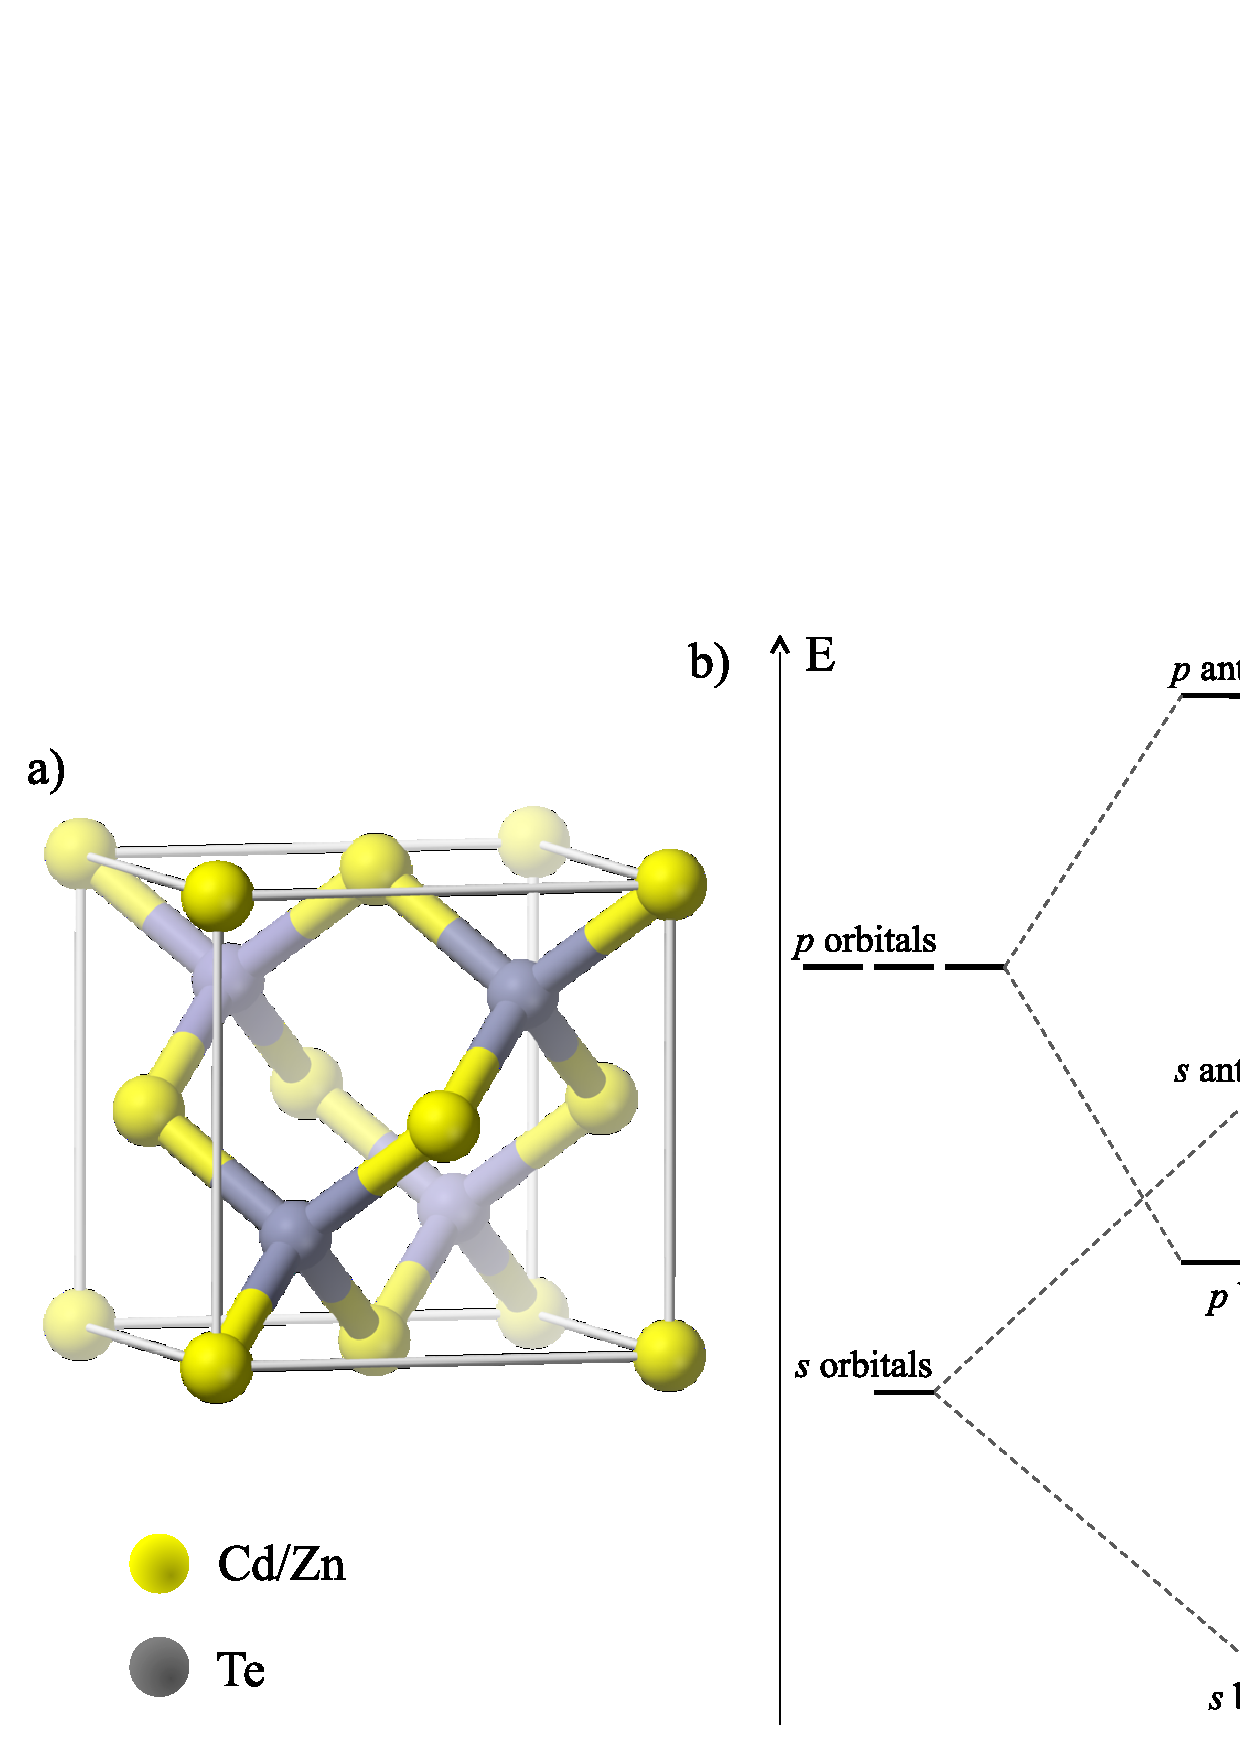
\includegraphics[width=13cm]{01-QD/Pictures/CrystalAndHybridization.png}
	\end{center}}
	\end{figure}

	The external orbitals for the cation are $s$ (4$d^{10}$5$s^2$ for Cd,  3$d^{10}$4$s^2$ for Zn) and $p$ for the anion (4$d^{10}$5$s^2$5$p^4$ for Te). In the crystal, their orbitals hybridize to form the conduction band and the valence band of the semiconductor. A good and more simple picture of this construction can be given considering the hybridization of two elements of the column IV of the periodic table. It is the well-known $sp$-hybridization. A single unit of the crystal contains 8 valence electrons, coming from the $s$ and $p$ levels of the ions. The $s$ and $p$ orbitals of these atoms hybridize to form 8 levels, 4 bonding and 4 anti-bonding.
	
	The lowest band of the bonding levels, coming from $s$ orbitals, will be filled by 2 valence electrons. 6 will be taken to fill the three bonding bands of higher energy, formed by the hybridization of $p$ orbitals. Those bonding states form the valence band. At higher energy, the anti-bonding states form the conduction band. Since all the available electrons are used to fill the valence band, the conduction band is empty in the ground state. The lower energy band of the conduction band is formed by the anti-symmetric combination of the $s$ orbitals. At higher energy, the anti-symmetric hybridization of $p$ orbitals form three other bands.

	The energy needed to excite one electron from the higher energy state of the valence band to the lower energy state of the conduction band is called the gap. The gap is really important for the opto-electric properties of the semiconductor. In the ZnTe and CdTe cases, they are equal to $E_{g, ZnTe} = 2.40$ eV and  $E_{g, CdTe} = 1.60$ eV at 5K~\cite{FurdynaDMS}.
	
	The promotion of an electron to the conduction band leave in the valence band a quasi-particule called a hole. The hole represents the absence of an electron, and has thus the opposite characteristic (spin, charge, wave vector...) as the missing electron. Aside from the promotion of an electron to the conduction band, holes can also be injected in the semiconductor via the introduction of p-type defect.
	
	\begin{figure}[h!]
	\caption{Different type of heterojunctions between two semiconductors.\label{SCType}}
	{\begin{center}
		\includegraphics[width=14cm]{01-QD/Pictures/SCType.png}
	\end{center}}
	\end{figure}	
	
	When growing two semiconductors of different band gap on top of each other, a band offset appears at the interface. This offset is distributed between the valence band and the conduction band. It can be distributed in three different ways, depending of the relative energies of the conductions bands and valence bands. Those configurations are illustrated in Fig.~\ref{SCType}. CdTe grown over ZnTe is a type I semiconductor. In this case, both the electrons and the holes are confined in the semiconductor of smaller gap (since holes have the opposite energies as the missing electrons, they are confined in the higher energy part of the valence band). For CdTe on ZnTe, the valence band offset is of about 0.1 meV, about 5\% of the total offset~\cite{VBOZnTeCdTe}. The conduction band then takes most of the band gap offset. The confinement of the electrons in the conduction band is thus far more efficient than confinement of the hole.
	
		\subsubsection*{Band structure near the center of the Brillouin zone ($k = 0$)\label{k0Descr}}
			
	The optical properties of direct gap semiconductors such as CdTe and ZnTe are controlled by their symmetry at the center of the Brillouin zone, corresponding to an electron wave vector $\mathbf{k} = 0$. At this point, the conduction band has the $T_d$ group $\Gamma_6$ symmetry. As discussed, this band comes from the overlap of atomic $s$ orbitals, meaning the conduction electron will have no orbital momentum, and a total angular momentum $J = \dfrac{1}{2}$.
	
	The valence band is formed from $p$ orbitals, presenting a orbital momentum $L = 1$. It couples at $k = 0$ with the electron spin $S = 3/2$ through the spin-orbit coupling. $\mathbf{L}$ and $\mathbf{S}$ are then not good quantum number anymore. We can show that $\mathbf{J} = \mathbf{L}+ \mathbf{S}$, however, commute the hamiltonian presented in the following sections. This composition gives two sub-bands of total angular momentum $J = 1/2$ and $J = 3/2$. In the $T_d$ group, the quadruplet $J = 3/2$ is of $\Gamma_8$ symmetry, and the doublet $J = 1/2$ is of $\Gamma_7$ symmetry. Those bands are split by the spin-orbit interaction, with an energy $\Delta_{SO}$. The eigenstates $J^2$, $J_z$ are chosen as a basis for the system at $k = 0$.
	
	The conduction band and valence band states can now be written from the composition of the two uncoupled basis:
	\begin{align}	
		\Gamma_6&:
			\label{eBasis}
			\def\arraystretch{2.0}
			\begin{array}{lll}
				u_{\Gamma_6, \frac{1}{2}} &= |\dfrac{1}{2}, \dfrac{1}{2}\rangle &= |S\rangle|\uparrow\rangle \\
				u_{\Gamma_6, -\frac{1}{2}} &= |\dfrac{1}{2}, -\dfrac{1}{2}\rangle &= |S\rangle|\downarrow\rangle
			\end{array}
	\end{align}
	\begin{align}
		\Gamma_8&:
			\label{hBasis}
			\def\arraystretch{2.0}
			\begin{array}{lll}
				u_{\Gamma_8, \frac{3}{2}} &= |\dfrac{3}{2}, \dfrac{3}{2}\rangle &= |1\rangle|\uparrow\rangle \\
				u_{\Gamma_8, \frac{1}{2}} &= |\dfrac{3}{2}, \dfrac{1}{2}\rangle &= \sqrt{\dfrac{2}{3}}|0\rangle|\uparrow\rangle + \sqrt{\dfrac{1}{3}}|1\rangle|\downarrow\rangle \\	
				u_{\Gamma_8, -\frac{1}{2}} &= |\dfrac{3}{2}, -\dfrac{1}{2}\rangle &= \sqrt{\dfrac{2}{3}}|0\rangle|\downarrow\rangle + \sqrt{\dfrac{1}{3}}|1\rangle|\uparrow\rangle \\	
				u_{\Gamma_8, -\frac{3}{2}} &= |\dfrac{3}{2}, -\dfrac{3}{2}\rangle &= |-1\rangle|\downarrow\rangle \\	
			\end{array} \\
		\nonumber \\
		\Gamma_7&:
			\def\arraystretch{2.0}
			\begin{array}{ll}
				|\dfrac{1}{2}, \dfrac{1}{2}\rangle &= \sqrt{\dfrac{2}{3}}|1\rangle|\downarrow\rangle - \sqrt{\dfrac{1}{3}}|0\rangle|\uparrow\rangle \\
				|\dfrac{1}{2}, -\dfrac{1}{2}\rangle &= -\sqrt{\dfrac{2}{3}}|-1\rangle|\uparrow\rangle + \sqrt{\dfrac{1}{3}}|0\rangle|\downarrow\rangle
			\end{array}
	\end{align}
with:
	\begin{align*}
		|1\rangle &= -\frac{|X\rangle + i |Y\rangle}{\sqrt{2}} \\
		|0\rangle &= |Z\rangle \\
		|-1\rangle &= \frac{|X\rangle - i |Y\rangle}{\sqrt{2}}
	\end{align*}
where $|X\rangle$, $|Y\rangle$ and $|X\rangle$ are the wave function of the valence band top at $k = 0$. They are calculated from the hybridization of the atomic orbital $p_X$, $p_Y$ and $p_Z$.

	
		Since $\Delta_{SO} \simeq 0.9$ eV for CdTe and ZnTe, the $\Gamma_7$ band is far enough in the valence band to be able to limit our study to the interaction between the $\Gamma_6$ and $\Gamma_8$ bands. The electrons in the conduction band have a spin $\sigma = \frac{1}{2}$. The spin operator can therefore be written using the Pauli matrices. For a quantization along the growth axis of the semiconductor, noted $z$:
	\begin{align}
			\sigma_x = \dfrac{1}{2}
						\begin{pmatrix}
							0 & 1 \\
							1 & 0
						\end{pmatrix} \qquad ; \qquad
			\sigma_y = \dfrac{1}{2}
						\begin{pmatrix}
							0 & -i \\
							i & 0
						\end{pmatrix} \qquad ; \qquad
			\sigma_z = \dfrac{1}{2}
						\begin{pmatrix}
							1 & 0 \\
							0 & -1
						\end{pmatrix}
	\end{align}
In the same way, we can define the operators at the top of the valence band. For an angular momentum $J = \frac{3}{2}$ quantized along the $z$ axis, we have in the basis $(3/2, 1/2, -1/2, -3/2)$:
	\begin{align}
		\label{holeAngMom}
		\begin{array}{ccl}
			J_x = \begin{pmatrix}
						0 & \frac{\sqrt{3}}{2} & 0 & 0 \\
						\frac{\sqrt{3}}{2} & 0 & 1 & 0 \\
						0 & 1 & 0 & \frac{\sqrt{3}}{2} \\
						0 & 0 & \frac{\sqrt{3}}{2} & 0
					\end{pmatrix} & ; &
			J_y = i\begin{pmatrix}
						0 & -\frac{\sqrt{3}}{2} & 0 & 0 \\
						\frac{\sqrt{3}}{2} & 0 & -1 & 0 \\
						0 & 1 & 0 & -\frac{\sqrt{3}}{2} \\
						0 & 0 & \frac{\sqrt{3}}{2} & 0
					\end{pmatrix}
		\end{array} \nonumber \\
		 J_z = \begin{pmatrix}
						\frac{3}{2} & 0 & 0 & 0 \\
						0 & \frac{1}{2} & 0 & 0 \\
						0 & 0 & -\frac{1}{2} & 0 \\
						0 & 0 & 0 & -\frac{3}{2}
					\end{pmatrix} \qquad \qquad \qquad \qquad \quad \; \;
	\end{align}

Finally, for any spin operator $O$ ($O = \bm{\upsigma}$, $\mathbf{J}$ or any other angular momentum operator of this document), we can define the ladder operator, flipping the considered spin by one unit, such as $O_+|O\rangle \propto |O+1\rangle$ and $O_-|O\rangle \propto |O-1\rangle$. They read in the general case as:
	\begin{align}
		O_+ = O_x + iO_y \\
		O_- = O_x - iO_y
	\end{align}

	We are mainly interested in two light matter interaction in the semiconductor:  absorption of a photon of energy equal to or higher than the band gap by an electron of the valence band to reach the conduction band; or emission of photon by an electron relaxing from the conduction band to the valence band. However, angular momentum conservation rules forbid some transitions. In order to find them, we consider the coupling between a conduction band electron $|\Psi_c\rangle$ and a valence band hole $|\Psi_v\rangle$ through, in the dipolar approximation, the hamiltonian ${\cal H}_{dip} = -\mathbf{d}.\mathbf{E}$ with $\mathbf{d}$ the dipole operator and $\mathbf{E}$ the electric field, that can also be written ${\cal H}_{dip} = -\frac{e}{m}\mathbf{p}.\mathbf{A}$ with $\mathbf{p}$ the electron momentum and $\mathbf{A}$ the potential vector~\cite{RosencherOptoElec}. In this section, we go with the later. We then get:
	\begin{align}
		\langle \Psi_v | {\cal H}_{AF} | \Psi_c \rangle \propto \langle u_{\Gamma_8, J_z} | \mathbf{p} | u_{\Gamma_6, \sigma_z} \rangle
	\end{align}
Considering that $|\uparrow\rangle$ and $|\downarrow\rangle$ are orthogonal states, we can easily deduce the authorized transitions:
	\begin{easylist}[itemize]
		& Between $| u_{\Gamma_6, +\frac{1}{2}} \rangle$ and $| u_{\Gamma_8, +\frac{3}{2}} \rangle$ (corresponding to a hole $J_z = -\frac{3}{2}$), coupled by $p_- = p_x - ip_y$, corresponding to a $\sigma-$ photon absorption or emission.
		& Between $| u_{\Gamma_6, -\frac{1}{2}} \rangle$ and $| u_{\Gamma_8, -\frac{3}{2}} \rangle$ (corresponding to a hole $J_z = +\frac{3}{2}$), coupled by $p_+ = p_x + ip_y$, corresponding to a $\sigma+$ photon absorption or emission.
		& Between $| u_{\Gamma_6, +\frac{1}{2}} \rangle$ and $| u_{\Gamma_8, -\frac{1}{2}} \rangle$ (corresponding to a hole $J_z = +\frac{1}{2}$) coupled via a $\sigma+$ photon absorption or emission.
		& Between $| u_{\Gamma_6, -\frac{1}{2}} \rangle$ and $| u_{\Gamma_8, +\frac{1}{2}} \rangle$ (corresponding to a hole $J_z = -\frac{1}{2}$) coupled via a $\sigma-$ photon absorption or emission.
		& Between $| u_{\Gamma_6, \pm\frac{1}{2}} \rangle$ and $| u_{\Gamma_8, \mp\frac{1}{2}} \rangle$ coupled via a $\pi_z$ photon absorption or emission.
	\end{easylist}
Those transitions are summarize on Fig.~\ref{SelectionRules}, with their respective relative probability calculated from the oscillator strength of each of these transitions.

	\begin{figure}[h!]
	\begin{center}
		\includegraphics[width=14.8cm]{01-QD/Pictures/SelectionRules.eps}
	\end{center}
	\caption{Selection rules for optical transitions between valence band and conduction band in a quantum well. They are presented in this confined environment in order to have a clear separation between the heavy holes ($J_z = \pm \frac{3}{2}$) and the light holes ($J_z = \pm \frac{1}{2}$). Circularly polarized transition are noted $\sigma\pm$ and $\pi_z$ stands for a linear polarization along $z$ axis.}
	\label{SelectionRules}
	\end{figure}


		\subsubsection*{$k \neq 0$: the $\mathbf{k}.\mathbf{p}$ approach}	
	
	The whole CdTe band structure is presented on Fig.~\ref{BandStruct}. We see that the maximum of the valence band and the minimum of the conduction band are both reached at the point $\Gamma$, center of Brillouin zone, corresponding to an electron wave vector $\mathbf{k} = 0$. This is characteristic of a direct band gap semiconductor. 
	
	Near this band edge, we can describe the curvature of the energy $E(\mathbf{k})$ of the band using an effective mass for the carrier on it:
	\begin{align}
		E_{\{c,v\}} (\mathbf{k}) = - \frac{(\hbar k)^2}{2m_{\{c,v\}}(\mathbf{k})}
	\end{align}		
	 As we move away from the $\Gamma$ point, the valence band split into two branches: the one with small curvature, meaning a high effective mass for the carriers on it, is called the heavy-hole (hh) band, while the one presenting the highest curvature and smallest effective mass is called the light-hole (lh) band.
	 
	\begin{figure}[h!]
	\begin{center}
		\includegraphics[width=11.5cm]{01-QD/Pictures/CdTeband.eps}
	\end{center}
	\caption{CdTe band structure}
	\label{BandStruct}
	\end{figure}

	One way to understand this evolution is to apply the $\mathbf{k}.\mathbf{p}$ approximation, as proposed by Kane in 1957~\cite{KaneBandkp}. This model gives an estimation of the electronic band structure starting from the exact solution of the Schrödinger equation at the center of the Brillouin. The hamiltonian to resolve is then :	
	\begin{align}
		\label{SchrödEq}
		\left(\frac{p^2}{2m_0} + U(\mathbf{r})\right)|\psi_{n,\mathbf{k}}\rangle = E_{n,\mathbf{k}} |\psi_{n,\mathbf{k}}\rangle
	\end{align}
with $n$ the band index, $\mathbf{p} = -i\hbar\mathbf{\nabla}$, $U(\mathbf{r})$ the potential of the crystal, $m_0$ the mass of a free carrier and $|\psi_{n,\mathbf{k}}\rangle$ the Bloch wave, separated between a periodic part $u_{n,\mathbf{k}} (\mathbf{r})$ and plane-wave part $\exp(i\mathbf{k}.\mathbf{r})$ as follow:
	\begin{align}
		|\psi_{n,\mathbf{k}}\rangle = u_{n,\mathbf{k}} (\mathbf{r}) \exp (i\mathbf{k}.\mathbf{r})\label{BlochWave}
	\end{align}
Using Eq.~\ref{BlochWave} and after development of the gradient of $\psi_{n, \mathbf{k}}$, it is possible to rewrite Eq.~\ref{SchrödEq} as a function of the periodic part only:
	\begin{align}
		\label{kpHamil}
		\left(\frac{p^2}{2m_0} + U(\mathbf{r}) + \frac{\hbar^2 k^2}{2m_0} + \frac{\hbar}{m_0}\mathbf{k}.\mathbf{p}\right)u_{n,\mathbf{k}} = E_{n,\mathbf{k}} u_{n,\mathbf{k}}
	\end{align}
	
	To find the solutions around $k = 0$, we develop the $u_{n,\mathbf{k}}$ on the basis of the $\{u_{n,0}\}_n$ as:
	\begin{align*}
		u_{n,\mathbf{k}} = \sum_{n'} c_{n'} u_{n',0}
	\end{align*}
Assuming that the $u_{n,0}$ are known, we can calculate the matrix elements of Eq.~\ref{kpHamil}.
The resolution of this hamiltonian is often done in the books~\cite{kpMethod}, and gives, taking into account the $\Gamma_6$ and $\Gamma_8$ bands only:
	\begin{align}
		\begin{array}{l}
		E_c (k_z) = E_c + \dfrac{\hbar^2 k_z^2}{2m_c} \\
		E_{v, \pm\frac{1}{2}} (k_z) = E_v - \dfrac{\hbar^2 k_z^2}{2m_{lh}} \\
		E_{v, \pm\frac{3}{2}} (k_z) = E_v + \dfrac{\hbar^2 k^2_z}{2m_{0}}
		\end{array}	
	\end{align}
with $E_c$ (respectively, $E_v$) the energy of the conduction band (respectively, the valence band), $m_c$ the effective mass of the carrier in the conduction band and $m_{lh}$ the effective mass of the light hole. One can see that the splitting of the valence band separate the carrier with a spin $J_z = \pm \frac{3}{2}$ (hh) from the one with a spin $J_z = \pm \frac{1}{2}$ (lh). However, the hh presents a positive curvature in this results, meaning a positive effective mass. This contradict the schema given on Fig.~\ref{BandStruct}. Taking into account the coupling with the higher energy band, hh are found to have indeed a negative curvature~\cite{kpMethod}. Considering only two bands is too rough to really model the system.

		\subsubsection*{$k \neq 0$: the Luttinger hamiltonian}

	Another way to obtain the matrix describing the $\Gamma_8$ band is to use symmetry consideration. Luttinger showed in 1956~\cite{LuttingerHam} that the only Hamiltonian fulfilling the cubic symmetry is:
	\begin{align}
	\label{LuttHamil}
		{\cal H}_L = - \frac{h^2}{2m_0}\left(\gamma_1 k^2 I_4 - 2 \gamma_2 \sum_i k_i^2 \left(J_i^2 - \frac{1}{3} J^2\right) - 2 \gamma_3 (k_x k_y (J_x J_y + J_y J_x) + c.p.) \right)
	\end{align}
with $\gamma_1$, $\gamma_2$ and $\gamma_3$ the Luttinger parameters, $I_4$ the 4 $\times$ 4 identity matrix, $\mathbf{k}$ a vector of the Brillouin zone, $\mathbf{J}$ the angular momentum operator with $J_x$, $J_y$ and $J_z$ being 4 $\times$ 4 matric satisfying $[J_x, J_y] = iJ_z$ and circular permutation ($c.p$), such as the one defined on Eq.~\ref{holeAngMom}. 
	This hamiltonian can be simplified using the parameters:
	\begin{align}
		\begin{array}{l}
			A = \gamma_1 + \dfrac{5}{2} \gamma_2 \\
			B = 2 \gamma_2 \\
			C = 2(\gamma_3 - \gamma_2)
		\end{array}
	\end{align}
The Luttinger hamiltonian can then be rewritten:
	\begin{align}
		{\cal H}_L = - \frac{h^2}{2m_0}(Ak^2 I_4 - B(\mathbf{k}.\mathbf{J})^2 + C(k_x k_y (J_x J_y + J_y J_x) + c.p.))
	\end{align}
The $B$-term lifts the degeneracy of the $\Gamma_8$ band into two lh and hh sub-bands, and is invariant under arbitrary rotations. The $C$-term describes the warping of the valence band.

	In the spherical approximation, the Luttinger hamiltonian has two eigenvalues, giving us the value of the lh and hh effective mass:
	\begin{align}
		\begin{array}{l}
			E_{hh} = - \dfrac{\hbar^2 k^2}{2m_0 (A-2.25B)^{-1}} = - \dfrac{\hbar^2 k^2}{2m_0 (\gamma_1 - 2 \gamma_2 )^{-1}} = - \dfrac{\hbar^2 k^2}{2m_{hh}} \\
			E_{lh} = - \dfrac{\hbar^2 k^2}{2m_0 (A-0.25B)^{-1}} = - \dfrac{\hbar^2 k^2}{2m_0 (\gamma_1 + 2 \gamma_2 )^{-1}} = - \dfrac{\hbar^2 k^2}{2m_{lh}}
		\end{array}
	\end{align}
We find that the hh presents a negative curvature, as was found in other works~\cite{kpMethod}.

	The parameters and carriers effective masses are given in the Tab.~\ref{Param}.
	
	\begin{table} \centering
		\setlength\extrarowheight{2pt}
		\label{Param}
		\begin{tabular}{m{3cm}|m{3cm}|m{3cm}}
			\hline \hline
			 & \multicolumn{1}{c|}{CdTe} & \multicolumn{1}{c}{ZnTe} \\
			\hline \hline
			$E_g$ & 1606 meV & 2391 meV \\
			\hline
			$\varepsilon_r$ & 10.6 & 9.7 \\
			\hline
			$a_0$ & 6.48 \AA & 6.10 \AA \\
			\hline
			$\Delta_{SO}$ & 0.90 eV & 0.91 eV \\
			\hline
			$\gamma_1$ & 4.8 & 4.07 \\
			\hline
			$\gamma_2$ & 1.5 & 0.78 \\
			\hline
			$\gamma_3$ & 1.9 & 1.59 \\
			\hline
			$m_{hh, z}$ & 0.556 & 0.398 \\
			\hline
			$m_{hh, \bot}$ & 0.159 & 0.206 \\
			\hline
			$m_{lh, z}$ & 0.128 & 0.178 \\
			\hline
			$m_{lh, \bot}$ & 0.303 & 0.303 \\
			\hline
			$m_e$ & 0.096 & 0.116 \\
			\hline
		\end{tabular}
		\caption{Physical parameters for CdTe and ZnTe.}
	\end{table}
	
	In matrix form, using the basis ($u_{\Gamma_8, +\frac{3}{2}}$, $u_{\Gamma_8, +\frac{1}{2}}$, $u_{\Gamma_8, -\frac{1}{2}}$, $u_{\Gamma_8, -\frac{3}{2}}$), the Luttinger hamiltonian can be written as:
	\begin{align}
	\label{HLMat}
		{\cal H}_L = - \frac{\hbar^2}{2m_0}
		\begin{pmatrix}
			a_{hh} & b_{Lutt} & c_{Lutt} & 0 \\
			b_{Lutt}^* & a_{lh} & 0 & c_{Lutt} \\
			c_{Lutt}^* & 0 & a_{lh} & -b_{Lutt} \\
			0 & c_{Lutt}^* & -b_{Lutt}^* & a_{hh}
		\end{pmatrix}
	\end{align}
with:
	\begin{align*}
		a_{hh} &= (\gamma_1 - 2 \gamma_2)k_z^2 + (\gamma_1 + \gamma_2)k_{\parallel}^2 \\
		a_{lh} &= (\gamma_1 + 2 \gamma_2)k_z^2 + (\gamma_1 - \gamma_2)k_{\parallel}^2 \\
		b_{Lutt} &= -2\sqrt{3} \gamma_3 (k_x - ik_y)k_z \\
		c_{Lutt} &= - \sqrt{3}(\gamma_2 (k_x^2 - k_y^2) - 2i\gamma_3k_xk_y)
	\end{align*}


		\subsection{Lattice mismatch and the Bir-Pikus Hamiltonian \label{BPSec}}
		
	ZnTe crystal has a lattice parameter of $a_{ZnTe} = $ 6.10 \AA, while CdTe one is of $a_{CdTe} = $ 6.48 \AA. Since we grow CdTe on a ZnTe substrate epitaxially, this lattice mismatch results in strain in a CdTe layer grown on a ZnTe substrate:
		\begin{align}
			\varepsilon_{\parallel} = \frac{a_{ZnTe} - a_{CdTe}}{a_{CdTe}} = -5.8\%
		\end{align}
		
		In order to represent this strain and see its effects on the bands, we need to define a hamiltonian representing them. Strains deform the structure, so let's begin the representation with a volume $V = x\mathbf{u_x} + y\mathbf{u_y} + z\mathbf{u_z}$, with $(\mathbf{u_x}, \mathbf{u_y}, \mathbf{u_z})$ an orthonormal basis. This volume will transform into another one $V' = x\mathbf{u_x'} + y\mathbf{u_y'} + z\mathbf{u_z'}$, where, for $\varepsilon_{ij}'$ an expansion of the vector $i$ in the direction $j$:
		\begin{align}
			\begin{array}{l}							
				\mathbf{u_x'} = (1 + \varepsilon_{xx}')\mathbf{u_x} + \varepsilon_{xy}' \mathbf{u_y} + \varepsilon_{xz}' \mathbf{u_z} \\
				\mathbf{u_y'} = \varepsilon_{yx}' \mathbf{u_x} + (1 + \varepsilon_{yy}')\mathbf{u_y} + \varepsilon_{yz}' \mathbf{u_z} \\
				\mathbf{u_z'} = \varepsilon_{zx}' \mathbf{u_x} + \varepsilon_{zy}' \mathbf{u_y} + (1 + \varepsilon_{zz}')\mathbf{u_z}
			\end{array}
		\end{align}

	They are small deformation of the lattice, so we choose $|\varepsilon_{ij}'| \ll 1$. Such transformation can be decomposed in a symmetric part, the strain tensor, and an antisymetric one. We note the strain tensor $\overline{\overline{\varepsilon}}$, defined such as:
	\begin{align}
		\varepsilon_{ ii} &= \varepsilon_{ii}' \\
		\varepsilon_{ij} &= \frac{1}{2} \left(\varepsilon_{ij}' + \varepsilon_{ji}'\right)
	\end{align}

	In the linear regime, the strain tensor $\overline{\overline{\varepsilon}}$ is proportional to the stress tensor $\overline{\overline{\sigma}}$, where $\sigma_{ij}$ describe a force parallel to $i$ applied on a surface perpendicular to $j$. Therefore, $\sigma_{ii}$ will describe an elongation or compression stress, while $\sigma_{ij}$ ($i\neq j$) represents a shear stress. Since these tensor are symmetric, we can reduce the number of coefficient from nine to six: $\sigma_{xx}$, $\sigma_{yy}$, $\sigma_{zz}$, $\sigma_{xy} = \sigma_{yx}$, $\sigma_{xz} = \sigma_{zx}$ and $\sigma_{yz} = \sigma_{zy}$. Since $x$, $y$ and $z$ are physically equivalent, as well as $xy$, $xz$ and $yz$, only two diagonal coefficient are needed: $C_{11}$ and $C_{44}$. In the linear regime and for a cubic crystal, we can now write the Hooke's law:
	\begin{align}
	\label{HookeLaw}
		\begin{bmatrix}
			\sigma_{xx} \\
			\sigma_{yy} \\
			\sigma_{zz} \\
			\sigma_{xy} \\
			\sigma_{xz} \\
			\sigma_{yz}
		\end{bmatrix}
		=
		\begin{bmatrix}
			C_{11} & C_{12} & C_{12} & 0 & 0 & 0 \\
			C_{12} & C_{11} & C_{12} & 0 & 0 & 0 \\
			C_{12} & C_{12} & C_{11} & 0 & 0 & 0 \\
			0 & 0 & 0 & 2C_{44} & 0 & 0 \\
			0 & 0 & 0 & 0 & 2C_{44} & 0 \\
			0 & 0 & 0 & 0 & 0 & 2C_{44}
		\end{bmatrix}
		\begin{bmatrix}
			\varepsilon_{xx} \\
			\varepsilon_{yy} \\
			\varepsilon_{zz} \\
			\varepsilon_{xy} \\
			\varepsilon_{xz} \\
			\varepsilon_{yz}
		\end{bmatrix}
	\end{align}
These coefficient coupling strains in a direction to a force in the same direction are obviously positive.

	When the aforementioned cube is compressed in one direction (e.g. $\varepsilon_{zz} < 0$), it will expand in the other direction in order to minimize elastic energy ($\varepsilon_{xx}$, $\varepsilon_{yy} > 0$ in the example). If we do not allow strain in these other directions ($\varepsilon_{xx} = \varepsilon_{yy} = 0$), a stress in the x and y directions had to be applied to keep the cube from expanding in these directions ($\sigma_{xx}$, $\sigma_{yy} < 0$ in the example). We can therefore physically expect $C_{12} > 0$.
	
	The strain hamiltonian can be constructed noticing that the strain tensor $\overline{\overline{\varepsilon}}$ induces a shift in the energy band, and that any $\varepsilon_{ij}$ has the same symmetry as $k_i k_j$. The hamiltonian should then be formarly identical to the Luttinger hamiltonian. In the $\Gamma_8$ subspace, we can then use the Luttinger Hamiltonian, written in Eq.~\ref{LuttHamil}, replacing the $k_i k_j$ by $\varepsilon_{ij}$. We obtain the Bir-Pikus Hamiltonian by replacing the $\gamma_j$ parameters by the Bir-Pikus parameters $a_{\nu}$, $b$ and $d$ for the four levels at the top of the valence band~\cite{kpMethod}:
	\begin{align}
	\label{BPHamil}
		{\cal H}_{BP} = a_{\nu} \varepsilon + b \sum_i \varepsilon_{ii} \left(J_i^2 - \frac{1}{3}J^2\right) + \frac{2d}{\sqrt{3}} \sum_{i>j} \varepsilon_{ij} \{J_i J_j\}
	\end{align}
with $\varepsilon = Tr(\overline{\overline{\varepsilon}}) = \varepsilon_{xx} + \varepsilon_{yy}+ \varepsilon_{zz}$ and $\{J_i J_j\} = \frac{1}{2}(J_iJ_j + J_jJ_i)$

	The $a_{\nu}$ term, called the hydrostatic term, shifts the $\Gamma_8$ energy. In case of non-equal $\varepsilon_{ii}$ (shear strains), the $b$ term will split the two $\Gamma_8$ sub-bands as did a $k\neq 0$ in the Luttinger hamiltonian. The $d$ term, the pure shear strain (i.e $\varepsilon_{ij}$ with $i \neq j$), has the same effect on the $\Gamma_8$ band. For CdTe, Bir-Pikus parameter are $a_{\nu} = 0.91$ eV, $b = -1.0$ eV and $d = -4.4$ eV~\cite{CdTeBPCoef}.
	
	One can notice that the Bir-Pikus hamiltonian is completely independant from $\mathbf{k}$, meaning that the valence band hamiltonian of a strain semiconductor is simply the sum of the Luttinger hamiltonian ${\cal H}_L$ (Eq.~\ref{LuttHamil}) and the Bir-Pikus hamiltonian ${\cal H}_{BP}$ (Eq.~\ref{BPHamil}).
	
	Let see how this apply to a CdTe layer deposited on a ZnTe layer. As previously, we define $z$ as the growth direction. Since both semiconductors crystallize in a cubic lattice, the strains are the same in the $x$ and $y$ direction. We can then write the strains in the $xy$ plane:
	\begin{align}
	\label{epsperp}
		\varepsilon_{xx} = \varepsilon_{yy} = \varepsilon_{\parallel} = \frac{a_{ZnTe} - a_{CdTe}}{a_{CdTe}}
	\end{align}
In the $z$ direction, however, no stress applies: the crystal is free to expand in this direction in order to reduce the elastic energy. Therefore, we can write $\sigma_{zz} = 0$ and, according to Hooke's law in Eq.~\ref{HookeLaw}:
	\begin{align}
		\begin{array}{rl}
			\sigma_{zz} &= C_{12} \varepsilon_{xx} + C_{12} \varepsilon_{yy} + C_{11} \varepsilon_{zz} \\
						&= 0
		\end{array}		
	\end{align}
Using equality \ref{epsperp}, we can then deduce:
	\begin{align}
	\label{epsz}
		\varepsilon_{zz} = - \frac{2C_{12}}{C_{11}} \varepsilon_{\parallel} = - \frac{2C_{12}}{C_{11}} \frac{a_{ZnTe} - a_{CdTe}}{a_{CdTe}}
	\end{align}
	
	Since we grow CdTe over a ZnTe substrate, the CdTe lattice is compressed in the plane, i.e. $\varepsilon_{\parallel} < 0$. Since $C_{11}$, $C_{12} > 0$ and $\varepsilon_{\parallel} < 0$ for CdTe over ZnTe (see Eq.~\ref{epsperp}), one can easily deduce that $\varepsilon_{zz} > 0$. In the hypothesis of no defect created by the lattice mismatch, all the other strain terms are equal to zero. We can then decompose this strain into two component: a hydrostatic part $\overline{\overline{\varepsilon_{hyd}}}$ describing the volume variation without breaking the cubic symmetry, and a shear part $\overline{\overline{\varepsilon_{sh}}}$ introducing an anisotropy, breaking this symmetry:
	\begin{align}
		\overline{\overline{\varepsilon_{hyd}}} &= \frac{1}{3}(\varepsilon_{xx} + \varepsilon_{yy} + \varepsilon_{zz})I_3 \\
		\overline{\overline{\varepsilon_{sh}}} &= \overline{\overline{\varepsilon}} - \overline{\overline{\varepsilon_{hyd}}}
	\end{align}
	
	One can notice that $Tr(\overline{\overline{\varepsilon_{hyd}}}) = Tr(\overline{\overline{\varepsilon}}) = \varepsilon$. Since in the case of a hydrostatic compression, such as for CdTe over ZnTe, $\varepsilon_{hyd} < 0$, we then have $\varepsilon < 0$ and, according to the Bir-Pikus hamiltonian (Eq.~\ref{BPHamil}), the gap of CdTe increase.
	
	Seeing that $\varepsilon_{ij} = 0$ for $i\neq j$, we can rewrite the Bir-Pikus hamiltonian without the shear strain term. Moreover, since $J^2 = J_x^2 + J_y^2 + J_z^2$ and $\varepsilon_{xx} = \varepsilon_{yy} = \varepsilon_{\parallel}$, we can simplify this hamiltonian to:
	\begin{align}
		{\cal H}_{BP, biax} = a_{\nu} \varepsilon I_4 + \frac{b}{3}(\varepsilon_{\parallel} - \varepsilon_{zz})(J_x^2 + J_y^2 - 2 J_z^2)
	\end{align}
And, since we are in the valence band with $J = \frac{3}{2}$ and $J_x^2 + J_y^2 + J_z^2 = J(J+1)I_4$, we can simplify the Bir-Pikus hamiltonian to its final form in the case of biaxal strains:
	\begin{align}
		{\cal H}_{BP, biax} = \left(a_{\nu} \varepsilon + \frac{5}{4} b (\varepsilon_{\parallel} - \varepsilon_{zz})\right)I_4 - b (\varepsilon_{\parallel} - \varepsilon_{zz})J_z^2
	\end{align}
	
	Using Eq.~\ref{epsperp} and \ref{epsz}, we can easily calculate $\varepsilon_{\parallel} - \varepsilon_{zz}$. Since $J_z|n\rangle = n|n\rangle$, we can find the hh/lh splitting:
	\begin{align}
		\begin{array}{rl}
			\Delta_{lh} = E_{\pm \frac{3}{2}} - E_{\pm \frac{1}{2}} &= - 2b \left(1 + \dfrac{2C_{12}}{C_{11}} \right) \dfrac{a_{ZnTe} - a_{CdTe}}{a_{CdTe}} \\
													&= 2b \left(1 + \dfrac{2C_{12}}{C_{11}} \right) \dfrac{a_{CdTe} - a_{ZnTe}}{a_{CdTe}}
		\end{array}
	\end{align}
We find that, in a fully strained CdTe layer over a ZnTe substrate, the hh band is 300 meV above the lh one, and we could thus neglect the lh bad in first approximation. However, to describe the valence band in QDs, one should take into account more complex effect, such as a coupling of the confined heavy hole with ground state light holes in the barriers~\cite{Couplinghhlhbarrier}, or the the effective reduction of hh/lh splitting due to supercoupling via a dense manifold of hh like QD states lying between the confined heavy hole and light hole levels~\cite{Supercouplinghhlh}. These effects can drastically change the hh/lh effective splitting, creating energy level between lh and hh ones and will be needed to understand the dynamics of a hole coupled to an atomic atom presented in Chap.~\ref{CoDynMn} and \ref{CrDyn}.

		\subsection{The quantum dot: confining the carrier in 3 dimensions\label{e-hIntQD}}
		
		Embedding a semiconductor in another one of larger band gap confines spatially the carriers in one or multiple directions. Using the procedure we will describe in Chap.~\ref{Growth}, we can create nanometre size island of CdTe in a ZnTe lattice, effectively confining electrons in all three directions. This lead to a quantization of the carriers energy levels and a discretization of the optical properties. This confinement being analogue to the Coulomb interaction of an isolated atom, such a structure is often dubbed "artificial atom". The hole and the electron also interact through the Coulomb interaction, consisting of an attractive term, shifting energy levels, and an exchange interaction (discussed in Sec.~\ref{ehExch}). The electron-hole system has a hydrogen-like behaviour and is called an exciton.

	\begin{figure}[h!]
	\fcapside{\caption{AFM image (AFM image (250 nm $\times$ 250 nm) of CdTe/ZnTe quantum dots before caping. The dot density is estimated to be in the $10^{10}$ dots.cm$^{-2}$ range.}\label{AFM}}
	{\begin{center}
		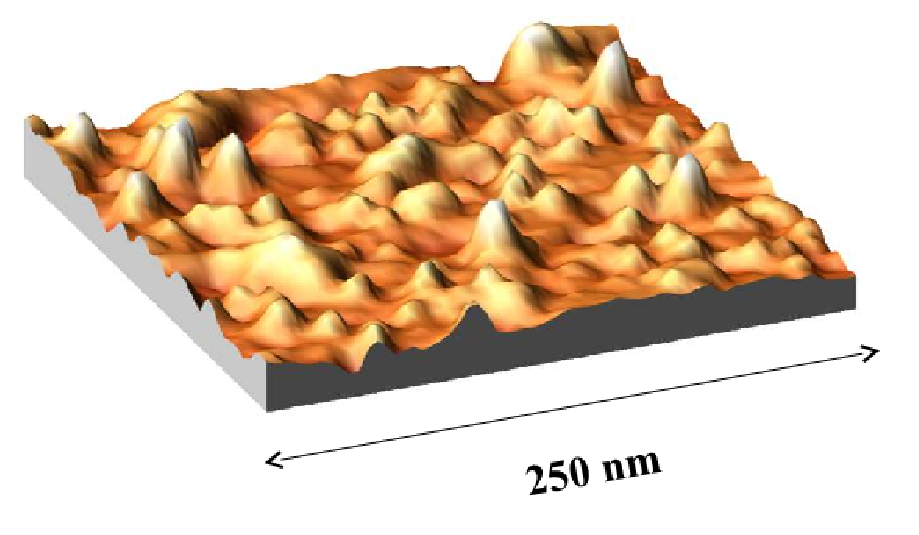
\includegraphics[width=8cm]{01-QD/Pictures/AFMQD.eps}
	\end{center}}
	\end{figure}

	The effects of confinement on the carrier are generally described in the envelop function formalism. To define these envelop functions, we develop the carriers wave-functions on all the Bloch states:
	\begin{align}
		\Psi (\mathbf{r}) = \sum_{n,\mathbf{k}} c_{n,\mathbf{k}} \psi_{n,\mathbf{k}} = \sum_{n,\mathbf{k}} c_{n,\mathbf{k}} u _{n,\mathbf{k}} (\mathbf{r}) \exp (i\mathbf{k}.\mathbf{r})
	\end{align}
Since we are in a confined environment, we can consider only the states around $\mathbf{k} = 0$. Since we consider the band extrema, we neglect for this part the inter-band wave function mixing and use the effective-mass approximation. We can then limit the expansion of Bloch state to an expansion on the $u _{n,0} (\mathbf{r}) \exp (i\mathbf{k}.\mathbf{r})$, with $n = \Gamma_6$ for the conduction band and $n = \Gamma_8$ for the valence band. The sum on $\Gamma_8$ is equivalent to a sum on the $J_z = \{\pm \frac{3}{2}, \pm \frac{1}{2}\}$. We can then write:
	\begin{align}
		\Psi_c (\mathbf{r}) & \simeq \sum_{\mathbf{k}} u _{\Gamma_6,0} c_{\Gamma_6, \mathbf{k}} (\mathbf{r}) \exp (i\mathbf{k}.\mathbf{r}) = u _{\Gamma_6,0} F_e (\mathbf{r}) \label{eEnvFunc} \\		
		\Psi_v (\mathbf{r}) & \simeq \sum_{J_z = \{\pm \frac{3}{2}, \pm \frac{1}{2}\}, k} u _{\Gamma_8,J_z} c_{J_z,\mathbf{k}} (\mathbf{r}) \exp (i\mathbf{k}.\mathbf{r})  = \sum_{J_z = \{\pm \frac{3}{2}, \pm \frac{1}{2}\}} u _{\Gamma_8,J_z} F_{J_z} (\mathbf{r}) \label{hEnvFunc}
	\end{align}
with $F_e (\mathbf{r}) = \sum_{\mathbf{k}} c_{\mathbf{k}} \exp (i\mathbf{k}.\mathbf{r})$ the electron envelop function and $F_{J_z} (\mathbf{r}) = c_{J_z,\mathbf{k}} \exp (i\mathbf{k}.\mathbf{r})$, $J_z = \{\pm \frac{3}{2}, \pm \frac{1}{2}\}$ the hole envelop functions.

	The effective mass approximation allows us to replace the periodic crystal potential and the free-electron kinetic energy by the effective hamiltonians representing the band extrema. Considering the effective mass is the same in CdTe and ZnTe, we can now work with the simple picture of an effective mass carrier with the envelop function defined in Eqs.~\ref{eEnvFunc} and \ref{hEnvFunc}, trapped in a potential $V_e (\mathbf{r})$ for the conduction band or $V_h (\mathbf{r})$ for the valence band, created by the band offset between the two semiconductors. We write the Schrödinger equations for these particles:
	\begin{align}
		\left(\frac{\hbar^2}{2m_e}\Delta \right)F_e (\mathbf{r}) + V_e (\mathbf{r}) F_e (\mathbf{r}) &= E_eF_e (\mathbf{r}) \label{eSchroding} \\
		(\tilde{{\cal H}}_L + \tilde{{\cal H}}_{BP} + V_h (\mathbf{r})) 
			\begin{pmatrix}
				F_{+ \frac{3}{2}} (\mathbf{r}) \\
				F_{+ \frac{1}{2}} (\mathbf{r}) \\
				F_{- \frac{1}{2}} (\mathbf{r}) \\
				F_{- \frac{3}{2}} (\mathbf{r})
			\end{pmatrix}
			&= E_h
			\begin{pmatrix}
				F_{+ \frac{3}{2}} (\mathbf{r}) \\
				F_{+ \frac{1}{2}} (\mathbf{r}) \\
				F_{- \frac{1}{2}} (\mathbf{r}) \\
				F_{- \frac{3}{2}} (\mathbf{r})
			\end{pmatrix}
			\label{hSchroding}
	\end{align}
with $\tilde{{\cal H}}_L$ and $\tilde{{\cal H}}_{BP}$ the hole hamiltonians. In particular, we have to take the opposite of the electron hamiltonian defined in Eq.~\ref{LuttHamil}. In $\tilde{{\cal H}}_L$, the $k$-terms transform into a gradient of the envelop function with the form $i\nabla$. For simplicity, the $\tilde{}$ will be dropped in the next equations. The derivation of the effective mass approximation can be found in reference \cite{LuttElecMotion}.

	As pointed out in the end of Sec.~\ref{BPSec}, the gap between lh and hh is of about 300 meV, wide enough to neglect the lh contribution in first approximation. This is called the heavy hole approximation, decoupling the four differential equations defined in Eq.~\ref{hSchroding}. Only the ground states $|\pm \frac{3}{2}\rangle$ are considered, with the effective mass given by the diagonal term of ${\cal H}_{L}$, noted $m_{h, \parallel}$ in the plane and $m_{h, z}$ along the growth axis. The spin operator $J_x$, $J_y$ and $J_z$ can then be redefined in the heavy-hole space as $j_x$, $j_y$, $j_z$, written with the Pauli matrices like $\sigma_x$, $\sigma_y$ and $\sigma_z$.
	
	Even with those two approximations, the problem is not solvable analytically. However, it is possible for some chosen potentials. Let's consider a lens like quantum dot, with a radius in the $xy$ plane, noted $\rho$, much larger than its height $L_z$. We can therefore define two different harmonic oscillators: a 2D oscillator $V_{c,v} (\rho)$ in the plane, and a 1D oscillator $V_{c,v} (z)$ along the growth axis:
	\begin{align}
		V_{c,v} (\rho) = 4 \Delta E_{c,v} \frac{\rho ^2}{L_z^2} \\
		V_{c,v} (z) = 4 \Delta E_{c,v} \frac{z^2}{L_z^2}
	\end{align}
with $\Delta E_{c,v}$ the band offset between the two conduction (resp. valence) bands. The potential of the whole quantum dot will then be $V_{c,v} (\mathbf{r}) = V_{c,v} (\rho) + V_{c,v} (z)$. Separating the potential in those two parts means we are searching for solution of the form $F(z, \rho, \theta) = \chi (z) \phi_{n,m} (\rho, \theta)$, with $\theta$ the angle between the position vector and the $x$ axis.

	We write the characteristic spatial width $\sigma$ and characteristic frequency $\omega$ of the 2D harmonic oscillator felt by the hole:
	\begin{align}
		\Sigma_{\rho}^h &= \sqrt{\frac{\hbar}{m_{h, \parallel} \omega_{\rho}^{h}}} \\
		\omega_{\rho}^{h} &= \sqrt{\frac{8\Delta E_{v}}{m_{h, \parallel} L_{\rho}^2}}
	\end{align}
We can write the same equality along $z$ replacing $\rho$ by $z$ and $m_{h, \parallel}$ by $m_{h,z}$. The same can be done for electron, replacing the  $m_{h, \parallel}$ or $m_{h,z}$ by $m_e$ and $E_v$ by $E_c$.

	We can find in textbook such as ref.~\cite{MecQBasvant} the eigenstates of a harmonic oscillator from which we can deduce the eigenstates for the ground state (GS) and the first two degenerated excited states. The first excited state is found to have an angular momentum $l_z = \pm 1$, and is then noted $Exc, \pm 1$. The envelop functions and energy are then found to be:
	\begin{align}
			& F_{c,v}^{GS} (z, \rho, \theta) = \frac{1}{(\sqrt{\pi}\Sigma_z)^{\frac{1}{2}}} \exp \left(- \frac{z^2}{2 \Sigma_z^2}\right) \frac{1}{(\sqrt{\pi}\Sigma_{\rho})^{\frac{1}{2}}} \exp \left(- \frac{\rho^2}{2 \Sigma_{\rho}^2}\right) \label{GSWF} \\
			& E_{e,h}^{GS} = \hbar \frac{\omega_z^{e,h} + \omega_{\rho}^{e,h}}{2} \\
		\nonumber \\
			& F_{c,v}^{Exc, \pm 1} (z, \rho, \theta) = \frac{1}{(\sqrt{\pi}\Sigma_z)^{\frac{1}{2}}} \exp \left(- \frac{z^2}{2 \Sigma_z^2}\right) \frac{1}{(\sqrt{\pi}\Sigma_{\rho})^{\frac{1}{2}}} \exp \left(- \frac{\rho^2}{2 \Sigma_{\rho}^2}\right) \frac{\rho}{\sigma_{\rho}} \exp (\pm i\theta) \label{ExcWF} \\
			& E_{e,h}^{Exc, \pm 1} = \hbar \frac{\omega_z^{e,h} + 3 \omega_{\rho}^{e,h}}{2}
	\end{align}
We see that these energy levels are quantized in a way looking like an isolated atom. In reference to the atomic notation, the ground state, lower energy level, is noted $S$ and the two first degenerated level are noted $P$, even though atomic p-states usually are 3 fold degenerated.

	One remarkable feature of the envelop functions is that both GS and the two first excited states present the same envelop along the $z$ axis. The cause is directly the symmetry of the QD: since $L_z \ll L_{\rho}$, $\omega_z^{e,h} \gg \omega_{\rho}^{e,h}$, and since $E_{osc.\ harmo.} = (n+\frac{1}{2})\hbar \omega$, the next possible envelop function along the $z$ axis is at higher energy than the next one in the plane. This geometry is also responsible for the 2 fold degeneracy of the $P$-states.
	
	Both the GS and the excited states are once again degenerated due to the spin of the electron and the hole. The electron is in the conduction band with the $\Gamma_6$ symmetry: its spin along the $z$ axis is $\sigma_z = \pm \frac{1}{2}$ (noted $|\uparrow\rangle$ for $+\frac{1}{2}$ and $|\downarrow\rangle$ for $-\frac{1}{2}$). Since we are in the hh approximation, considering that the lh are far enough from the band edge to be negligible, the hole spin can only take the values $J_z = \pm \frac{3}{2}$ (noted $|\Uparrow\rangle$ for $+\frac{3}{2}$ and $|\Downarrow\rangle$ for $-\frac{3}{2}$). As pointed ahead, the hole is defined with the opposed characteristic of the missing electron. For instance, a hole $|\Downarrow\rangle$ corresponds to the absence of a valence electron $\Psi_v (\mathbf{r}) = u_{\Gamma_8, \frac{3}{2}} (\mathbf{r}) F_{\frac{3}{2}} (\mathbf{r})$.
	
	From the selection rules found in Sec.~\ref{k0Descr}, we can see that the only excitons able to recombine optically in the hh approximation are either formed by an electron of spin $\sigma_z = -\frac{1}{2}$ and a hole of angular momentum $J_z = +\frac{3}{2}$ (exciton of total angular momentum $X_z = +1$, recombining in $\sigma+$ polarization), or an electron of spin $\sigma_z = +\frac{1}{2}$ and a hole of angular momentum $J_z = -\frac{3}{2}$ (exciton of total angular momentum $X_z = -1$, recombining in $\sigma-$ polarization). Excitons of total angular moment $X_z = \pm2$ (electron spin $\sigma_z = \pm\frac{1}{2}$ with hole spin $J_z = \pm \frac{3}{2}$ exists, but cannot recombine optically.
	
	The addition of envelop functions in the carriers wave function adds another selection term:
	\begin{align}
		|\langle \Psi_v | \mathbf{p} | \Psi_c \rangle |^2 = |\langle F_v | F_c \rangle |^2|\langle u_{\Gamma_8, J_z} | \mathbf{p} | u_{\Gamma_6, \sigma_z} \rangle |^2
	\end{align}
The first term is the overlap of the envelop function, making sure the hole and the electron are of the right state. For instance, a transition between a $S$ state of the valence band and a $P$ state in the conduction band is then forbidden. The second term is the same as the one studied earlier, and from which we deduced the selection rules.

	
	Approximating the QD potential as a harmonic potential usually overestimate the confinement, and thus the single-particle energy. But the wave-functions found in this chapter can still be used as trial wave-functions for variational calculations in other potential, in order to calculate the correct energy level.
	

		\subsection{Electron-hole exchange in quantum dots\label{ehExch}}
		













	%Bir et Pikus: l'interaction d'échange de coulomb de l'électron CB and les électrons VB peut être séparés en deux terme : un short range et un long range.
	
	Electrons are fermions, and thus are subjected to the Pauli exclusion principle. Being charged particles, they also interact with each other via the Coulomb interaction. Both of those have to be considered to write the interaction between the carriers in the semiconductor. It was shown by Wardzyński et al.~\cite{ExchSplitInteratomic} that the interaction between a conduction electron and all the electrons of the valence band can be written as an interaction between the considered electron and the corresponding hole. It can be separated into two terms: the direct Coulomb interaction, independent of the particles spins, and the exchange Coulomb interaction.
	
	
	In exciton, the direct Coulomb term is attractive, as classically expected from an electric interaction between two opposite charges. However, more complex systems can exist in a semiconductor: charged excitons X$^+$ (hole-hole-electron complex) and X$^-$ (hole-electron-electron complex), or biexciton X$^2$ (two excitons of opposite total angular momentum). Higher order multi-exciton or charged biexciton might also exists but they are not discussed in this thesis. In those multi-excitons, the total Coulomd interaction and the confinement make the system stable.

	Taking into account the symmetry of the crystal, Bir and Pikus demonstrated~\cite{BPExchInt} that the exchange hamiltonian between an electron of the conduction band and hole in the valence band can be decomposed in two different components:
	\begin{easylist}[enumerate]
		\ListProperties(Numbers=r, FinalMark={) })
		& For an electron and a hole in the same Brillouin zone, the short-range exchange interaction has to be considered. It can be written:
		\begin{align}
			\label{ShortRange}
			{\cal H}_{eh}^{sr} = I_{eh}^{sr} \bm{\upsigma}.\mathbf{j} + \sum_{i = x,y,z} b_i^{exch} \sigma_i j_i^3
		\end{align}
The first term lift the degeneracy between exciton of total angular moment $X=2$ and $X=1$. The second one takes into account the reduction of symmetry in a cubic lattice and gives the dark states a fine structure. This splitting is expected to be much smaller than the lift induced by $I_{eh}^{sr}$, but has never been observed experimentally in bulk semiconductor.
		& Carriers in different Brillouin-zone might be affected by the long-range exchange interaction. In bulk semiconductors, the long range term doesn't affect the bright exciton at $k = 0$. Since the radiative recombination we study occurs at $k=0$ in the studied semiconductors, the effects of the long range interaction are not visible via this probe.
	
	In a quantum dot, the confinement of the carrier leads to a better overlap of the wave function and thus greater short range exchange energies. Moreover, in an anisotropic potential, such as the one of Stransky-Krastanov dots (see Sec.~\ref{SK}), the long-range interaction mixes the bright excitons, splitting them in two levels. It is usually written as a $\delta_1$ term in the exchange hamiltonian.
	\end{easylist}
	%The splitting between the dark and bright excitons is thus also affected.

	Taking into account all these effects, we can the write the total exchange hamiltonian in the heavy hole exciton subspace ($X_z = |+2\rangle$, $|+1\rangle$, $|-1\rangle$, $|-2\rangle$):
	\begin{align}
	\label{Heh}
		{\cal H}_{eh} &= \frac{1}{2}
		\begin{pmatrix}
			\delta_0 & 0 & 0 & \delta_2 \\
			0 & - \delta_0 & \delta_1 \exp(-2i \phi_1) & 0 \\
			0 & \delta_1 \exp(2i \phi_1) & -\delta_0 & 0 \\
			\delta_2 & 0 & 0 & \delta_0
		\end{pmatrix}
	\end{align}
with $\delta_0 = \frac{3}{2}I_{eh}$, representing the splitting between dark and bright exciton, $I_{eh} < 0$ being the electron-hole exchange constant; $\delta_1$ the splitting between the bright exciton states; and $\delta_2$ the fine structure of the dark exciton states. $\delta_0$ value is controlled both by long-range and short-range interaction, and is typically about 1 meV in CdTe/ZnTe. $\delta_1$ only appears in anisotropic QDs and is induced by the long-range interaction, varying between a few tens and a few hundreds of $\mu$eV. Finally, $\delta_2$ primarily arise from the short-range interaction.

	
	Calculating the eigenstate of the hamiltonian \ref{Heh}, we find that the long range interaction induce a linear polarization of the PL of the optically active states along $\varphi_1$ and $\varphi_1 + 90^{\circ}$ as follows:
	\begin{align}
		|\pi_{\varphi_1}\rangle = \frac{1}{\sqrt{2}}\left(\exp(-i\varphi_1)|+1\rangle + \exp(i\varphi_1)|-1\rangle\right) \\
		|\pi_{\varphi_1 + 90^{\circ}}\rangle = \frac{1}{\sqrt{2}}\left(\exp(-i\varphi_1)|+1\rangle - \exp(i\varphi_1)|-1\rangle\right)
	\end{align}
where $\varphi_1 = \dfrac{\pi}{4}$ corresponds to a polarization of the emission along the 110 axis.

	This model works well for quantum dots with an elongated lens shape ($C_{2v}$ symmetry), the shape taken for ideal QDs.  However, more realistic self-assembled QDs can have symmetries which can deviate quite substantially from the idealized shapes of circular or ellipsoidal lenses. For a $C_{s}$ symmetry (truncated ellipsoidal lens), additional terms coupling the dark and the bright excitons have to be included in the electron-hole exchange Hamiltonian. Following Ref. \cite{ZielinskiDarExc}, the general form of the electron-hole exchange Hamiltonian in the heavy-hole exciton basis for a low symmetry quantum dot (C$_s$) and a polarization along 110 is:
	\begin{align}
		\label{HehCs}
		\mathcal{H}_{eh} =\frac{1}{2} \left(
			\begin{array}{cccc}
			\delta_0                               &e^{-i\pi/4}\delta_{11}              &e^{i\pi/4}\delta_{12}        &\delta_2\\
			e^{i\pi/4}\delta_{11}                      &-\delta_0                       &e^{-i\pi/2}\delta_{1}       &-e^{i\pi/4}\delta_{12}\\
			e^{-i\pi/4}\delta_{12}                  &e^{i\pi/2}\delta_{1}           &-\delta_0                     &-e^{-i\pi/4}\delta_{11}\\
			\delta_2                 &-e^{-i\pi/4}\delta_{12}          &-e^{i\pi/4}\delta_{11}                     &\delta_0\\
			\end{array}
		\right)
\end{align}
		
		
		\subsection{Valence band mixing\label{VBM}}	
	
	We showed that the long range exchange interaction split the neutral exciton bright states in two linearly polarized lines, with a $90^{\circ}$ angle between them. However, this simple picture doesn't fit well with the data, such as presented in Fig.~\ref{XAlLinPol}. It is clear for the neutral species (X, X$^2$) that the angle between the polarization of the two lines is different from $90^{\circ}$. Moreover, the charged species (X$^+$, X$^-$) are found to present linear polarization dependencies. In those systems, the presence of two carriers (hole for X$^+$, electron for X$^-$) with opposite spin cancel out the electron-hole exchange interaction. Their linear polarization dependencies arise then from another phenomena.
	
	\begin{figure}[h!]
	\begin{center}
		\includegraphics[width=13cm]{01-QD/Pictures/LinPol.png}
	\end{center}
	\caption{PL intensities of the bi-exciton (X$^2$), the charged excitons (X$^+$, X$^-$) and the neutral exciton (X) of a CdTe/ZnTe QD as the function of the angle of the linearly polarized detection. To simplify the reading, the intensities were also plotted on polar graph (bottom). Picture taken from Yoan L\'eger PhD thesis~\cite{YoanTh}.}
	\label{XAlLinPol}
	\end{figure}
	
	In order to understand the linear polarization dependency, we have include the light hole contribution. Looking at the general form of the Luttinger hamiltonian \ref{HLMat}, we see that it mixes heavy hole and light hole through its non-diagonal term $b_{Lutt}$ and $c_{Lutt}$. The Bir-Pikus hamiltonian \ref{BPHamil} presents the same symmetry and the same form as the Luttinger hamiltonian and thus also induces a coupling between the lh states and the hh states.
	
	In general, we can write the hamiltonian describing the influence of shape and strain on the valence structure in the ($|\dfrac{3}{2}, +\dfrac{3}{2}\rangle$, $|\dfrac{3}{2}, +\dfrac{1}{2}\rangle$, $|\dfrac{3}{2}, -\dfrac{1}{2}\rangle$, $|\dfrac{3}{2}, -\dfrac{3}{2}\rangle$) basis as:	
	\begin{align}
	\label{HVBM}
		{\cal H}_{VBM} =
		\begin{pmatrix}
			p+q & s & r & 0 \\
			s^* & p-q & 0 & r \\
			r^* & 0 & p-q & -s \\
			0 & r^* & -s^* & p+q
		\end{pmatrix}				
	\end{align}
The induced hh/lh mixing is called Valence Band Mixing (VBM).

	Supposing a VBM only caused by strain anisotropy, its parameters can be written as function of the Bir-Pikus parameters and the crystal strain $\varepsilon_{ij}$ ($i,j = x$, $y$, $z$). The VBM parameters then writes~\cite{kpMethod}:
	%with $x$ the (100) axis of the crystal lattice and $z$ as defined above
	\begin{align}
		\label{VBMParam}
		p 	&= a_v Tr(\varepsilon) \\
		q	&= b \left(\varepsilon_{zz} - \frac{\varepsilon_{xx} + \varepsilon_{yy}}{2}\right) \\
		r	&= b \frac{\sqrt{3}}{2} (\varepsilon_{xx} - \varepsilon_{yy}) - id \varepsilon_{xy} \\
		s	&= d(\varepsilon_{xz} - i\varepsilon_{yz})
	\end{align}
The splitting between the hh states and the lh states can now be calculated in function of the Bir-Pikus parameters:
	\begin{align}
		\begin{array}{rl}
			\Delta_{lh} &= E_{\pm\frac{3}{2}} - E_{\pm\frac{1}{2}} = (p+q) - (p-q) \\
						&= 2b \left(\varepsilon_{zz} - \dfrac{\varepsilon_{xx} + \varepsilon_{yy}}{2}\right)
		\end{array}
	\end{align}
	
	If we now suppose a system with pure in-plane strain anisotropy ($r \neq 0$ and $s=0$), for an origin of the energy at the top of the valence band, i.e. the hh band, we can rewrite the VBM hamiltonian in the same basis as above as:
	\begin{align}
		{\cal H}_{VBM}^{in\ plane} =
		\begin{pmatrix}
			0 & 0 & \rho_s\exp(-2i\theta_s) & 0 \\
			0 & \Delta_{lh} & 0 & \rho_s\exp(-2i\theta_s) \\
			\rho_s\exp(2i\theta_s) & 0 & \Delta_{lh} & 0 \\
			0 & \rho_s\exp(2i\theta_s) & 0 & 0
		\end{pmatrix}
	\end{align}
with $\rho_s$ the strain coupling amplitude and $\theta_s$ the angle between axis of the strain induced anisotropy in the QD plane and the $x$ axis. One can notice that in the case of pure in-plane anisotropy, $|+\dfrac{3}{2}\rangle$ only mixes with $|-\dfrac{1}{2}\rangle$ and $|-\dfrac{3}{2}\rangle$ with $|+\dfrac{1}{2}\rangle$. An anisotropy along the $z$ axis, growth axis of the dots, is needed to mix $|\pm \dfrac{3}{2}\rangle$ with $|\pm \dfrac{1}{2}\rangle$. With this notation, in the limit of weak VBM, we can now rewrite the ground state of the holes as pseudo-spin in order to take the hh/lh mixing into account:
	\begin{align}
		|\tilde{\Uparrow}\rangle \propto |+\frac{3}{2}\rangle - \frac{\rho_s}{\Delta_{lh}}\exp(2i\theta_s)|-\frac{1}{2}\rangle \\
		|\tilde{\Downarrow}\rangle \propto |-\frac{3}{2}\rangle - \frac{\rho_s}{\Delta_{lh}}\exp(-2i\theta_s)|+\frac{1}{2}\rangle
	\end{align}
And we can define new angular momentum operator for these pseudo-spin:
	\begin{align}
		\tilde{J}_+ &= \frac{\rho_s}{\Delta_{lh}}
			\begin{pmatrix}
				0 & -2\sqrt{3}\exp(-2i\theta_s) \\
				0 & 0
			\end{pmatrix} \label{JtildeUP} \\
		\tilde{J}_- &= \frac{\rho_s}{\Delta_{lh}}
			\begin{pmatrix}
				0 & 0 \\
				-2\sqrt{3}\exp(2i\theta_s) & 0
			\end{pmatrix} \label{JtildeDOWN} \\
		\tilde{J}_z &=
			\begin{pmatrix}
				\dfrac{3}{2} & 0 \\
				0 & -\dfrac{3}{2}
			\end{pmatrix} \label{JtildeZ}
	\end{align}
$\tilde{J}_{\pm}$ are the ladder operators, flipping the hole spin, whereas $\tilde{J}_z$ return the spin value. This last operator shows these states are mainly hh. This pseudo spin description is usually enough to understand the effect of the VBM, and we will use it to study how it modifies the emission of the quantum dot.

	%\end{align}

	In order to do so, we begin to consider the emission of the negatively charged state X$^-$. Since, as explained earlier, the exchange interaction is zero in such systems, because of the opposite spin of the two electrons, it will allow us to focus on the effects of the VBM. We can ignore the envelop function, testing mainly the overlap of the carriers wave function and thus not affecting the polarization of the emission. We write the polarization of the detection $\mathbf{e} = \cos (\alpha) \mathbf{e_x} + \sin (\alpha) \mathbf{e_y}$. We then can find the oscillator strength of the transition:
	\begin{align}		
		\begin{array}{rl}
		\label{VBMPolar}
			\Omega (\alpha) &\propto |\langle \uparrow | \cos(\alpha)p_X + \sin(\alpha)p_Y | \uparrow \downarrow \tilde{\Uparrow} \rangle |^2 \\
							&= 1 + \dfrac{1}{3} \dfrac{\rho_s}{\Delta_{lh}}^2 + \dfrac{2}{\sqrt{3}} \dfrac{\rho_s}{\Delta_{lh}} \cos(2(\theta_s - \alpha))
		\end{array}
	\end{align}
with $\mathbf{p} = -i\hbar\bm{\nabla}$. Contrary to what is expected in the hh approximation, we see that the charged exciton can have a strong linear component, depending on the strength of the lh/hh mixing.

	In the QD presented in Fig.~\ref{XAlLinPol}, the linear polarization rate $\rho_l = \dfrac{2A}{1 + A^2} \approx 40\%$, with $A = \frac{\rho_s}{\sqrt{3}\Delta_{lh}}$ corresponding to a very strong lh-hh mixing, with $\frac{\rho_s}{\Delta_{lh}} \approx 0.75$. Experimentally, no correlation were found between the polarization axis of different QDs, neither with the crystallographic axis, nor between QDs close to each other. Such a behaviour can be explained considering the anisotropic relaxation of strains occurring during the growth of the QDs~\cite{VBMArticle}. This behaviour was also observed in III-V compounds at low QD density (near the 2D-3D transition), also attributed to the effect of strains~\cite{IIIVFastExcSpinRelax}. For the III-V system, this hypothesis is supported by AFM studies showing that, in such growth conditions, the dots are preferentially nucleating near structural defects~\cite{IIIVAFM}. In the case of II-VI materials, a strained induced hh/lh mixing is not surprising as the dislocation formation energy is lower in those material, as shown in Ref.~\cite{TinjodMBE}.

	For the charged states $X^+$ and $X^-$, only the VBM leads to this linear polarization. However, in $X$ and $X^2$, the VBM and the long range exchange interaction are in competition for the polarization of the emission. The strain tends to polarize linearly the PL along $\theta_s$ and $\theta_s + 90^{\circ}$, when the long range exchange interaction favour linear emission along $\varphi_1$ and $\varphi_1 + 90^{\circ}$. This explains that the angle between the two linearly polarized exciton lines is not equal to $90^{\circ}$. Moreover, the valence band mixing results in a fine structure splitting through the short range exchange interaction that can either enhance or decrease the fine structure splitting due to the long range exchange interaction. In order to illustrate our point, we consider only the isotropic part of the short range electron-hole exchange interaction described in Eq.~\ref{ShortRange}:
	\begin{align}
		{\cal H}_{eh}^{sr,iso} = I_{eh} \bm{\upsigma}.\mathbf{J}
	\end{align}
where $\frac{3}{2}I_{eh}$ corresponds to the energy splitting between bright and dark excitons due to the short range exchange interaction. The coupling between the bright states $|\downarrow \tilde{\Uparrow}\rangle$ and $|\uparrow \tilde{\Downarrow}\rangle$ through ${\cal H}_{eh}^{sr,iso}$ can be calculated using the pseudo-spin ladder operator defined in \ref{JtildeUP} and \ref{JtildeDOWN}:
	\begin{align}
		\langle \downarrow \tilde{\Uparrow} | {\cal H}_{eh}^{sr,iso} | \uparrow \tilde{\Downarrow}\rangle = \frac{1}{2\sqrt{3}} I_{eh} \frac{\rho_s}{\Delta_{lh}} \exp(-2i\theta_s)
	\end{align}
	
	Hence, the valence band mixing through the short range exchange interaction splits the bright states into two linearly polarized states along axis defined by the strain angle $\theta_s$. The competition between this effect and the long range exchange interaction results in an angle between the two linearly polarized states different from $90^{\circ}$, as observed in the emission of CdTe/ZnTe QDs~\cite{DELum} and in InAs/GaAs ones~\cite{PolarIIIV}. Dark states are also coupled to bright ones in second order, giving them a weak oscillator strenght, with a dipole along $z$. A more in depth investigation of these effects was done in Yoan L\'eger's PhD thesis~\cite{YoanTh}.

	
	\section{Exchange interaction between carrier and magnetic atom\label{Exch}}
	
		\subsection{Exchange interaction in diluted magnetic semiconductors\label{ExchDMS}}
		
		We are interested in thesis to introduce a low density of either Manganese or Chromium atoms in the crystal. A semiconductor doped this way is called Diluted Magnetic Semiconductor (DMS). The magnetic atoms interact with the semiconductor electrons via its localized electrons on its outside $d$ shell, via the exchange interaction. In this thesis, we are at the limit of what is considered a DMS: the density of magnetic atom (Mn and Cr) is about the same of the density of QDs. This way, statistically a few QDs contains a single magnetic atom per QD. This system can be used as a spin {\em qbit}. For Mn and Cr in CdTe, the outside $d$ shell is the $d$ orbital, so it will be the one considered in the following. From the interactions between these electrons and the one in the conduction band of the semiconductor, new properties will arise. We will write in this section the interactions between the different electrons of the semiconductor as a "Heisenberg" interaction:
		\begin{align}
			{\cal H}_{Heisenberg} = I \bm{\upsigma}.\mathbf{S}
		\end{align}
with $I$ the interaction constant, $\bm{\upsigma}$ the electron spin and $\mathbf{S}$ the spin of the magnetic atom.
	
	This interaction represents the Pauli exclusion principle through the interaction between two spins. All the interactions in this section will be of this form, although representing different physical processes, with only the interaction constant $I$ varying from one to another.
	
		\subsubsection*{Hamiltonian of a DMS}
	
	Both Cr and Mn are close in size to the Cd atoms they replace, so their insertion only induces a small perturbation in the crystal structure, meaning the semiconductor wave function will not be significantly altered by them. We can then, as usual, write the conduction electron wave function as $|\psi_{\mathbf{k}}\rangle|\sigma;\sigma_z\rangle \equiv |\psi_{\mathbf{k}};\sigma_z\rangle$, $|\psi_{\mathbf{k}}\rangle$ being the Bloch function of the electron. In a first time, we only consider electrons of the conduction band. On the other side, considering a magnetic atom at $\mathbf{r} = \mathbf{R_d}$, we write the spatial component of the wave function $\Phi_d (\mathbf{r} - \mathbf{R_d})$. Its total electronic spin, sum of the electron spins on its $d$ orbital, is noted $|S; S_z\rangle$. The whole wave function of the magnetic atom is then $|\Phi_d;S_Z\rangle$.
	
	Let's first consider the hamiltonian for single magnetic atom. Using Born-Oppenheimer approximation, separating the movement of the electrons from the one of the nuclei, we can write the hamiltonian for these electrons:
	\begin{align}
	\label{BOHamil}
		{\cal H}_{BO} = \sum_i \left(\frac{p_i^2}{2m_c} + V_c (\mathbf{r}_i) \right) + \frac{1}{2} \sum_{i,j} \frac{e^2}{4\pi \varepsilon_0 |\mathbf{r_i} - \mathbf{r_j}|}
	\end{align}
The first term is a single particle hamiltonian, taking into account the kinetic energy of the electron and the crystal potential $V_c (\mathbf{r}_i)$ felt by the electron at the position $\mathbf{r}_i$. This potential includes the impurities' potential, meaning it will be different at the impurities positions rather than elsewhere in the semiconductor. The final term represents the Coulomb interaction between the electrons.

	We can rewrite this hamiltonian using second quantification. We define the destruction (resp. creation) operator of a particle in the conduction band at the wave vector $\mathbf{k}$ and the spin $\sigma$ as $a_{\mathbf{k}, \sigma}$ (resp. $a_{\mathbf{k}, \sigma}^{\dagger}$). In the same way, we define the destruction (resp. creation) operator of the electronic level of an impurity as $a_{d, S}$ (resp. $a_{d, S}^{\dagger}$). Assuming the number of electrons on the $d$ orbital of the considered magnetic atom does not change, the hamiltonian \ref{BOHamil} then becomes:
	\begin{align}
			{\cal H}_{SQ} &= \sum_{\mathbf{k}, \sigma} E_{\mathbf{k}} a_{\mathbf{k}, \sigma}^{\dagger} a_{\mathbf{k}, \sigma} + \sum_{S} E_d a_{d, S}^{\dagger} a_{d, S} + \sum_{\mathbf{k}, \mathbf{k}'} U_{\mathbf{k}, \mathbf{k}'} a_{\mathbf{k}, \sigma}^{\dagger} a_{\mathbf{k}', \sigma} \nonumber \\
								&\qquad\qquad\quad+ \sum_{\mathbf{k}, \sigma, S} V_{kd} (a_{\mathbf{k}, \sigma}^{\dagger} a_{d, S} + a_{d, S}^{\dagger} a_{\mathbf{k}, \sigma}) + \frac{1}{2} \sum_{i,j,m,n} V_{i,j,m,n} a_i^{\dagger} a_j^{\dagger} a_n a_m \label{HamilSQ} \\
						&= {\cal H}_0 + {\cal H}_d + V_d + {\cal H}_{hyb} + {\cal H}_{Coulomb} \nonumber
	\end{align}
with $E_{\mathbf{k}}$, $E_d$, $U_{\mathbf{k}, \mathbf{k}'}$, $V_{kd}$ and $V_{i,j,m,n}$ the interactions constant. The constant electron number assumption is good enough for the picture we want to draw since most of the spin-driven interactions do not induce a change of this number.

	${\cal H}_0$ represents the energy of the unperturbed wave function of the semiconductor, with $E_k$ the energy of an electron with the wave vector $\mathbf{k}$.
	
	${\cal H}_d$ is the same as ${\cal H}_0$ but for an electron of the $d$ orbital of the considered magnetic impurity, with $E_d$ the energy of an electron on this orbital.
	
	$V_d$ represents the impurity potential, allowing the semiconductor electrons to scatter on it. However, in II-VI materials, both Mn and Cr are isoelectric impurities. Their modification to the host semiconductor potential is therefore negligible~\cite{DyakonovSpinPhysicsSC} and $|\psi_k\rangle$ can still be used as solutions for the electrons of the semiconductor.
	
	${\cal H}_{hyb}$, also called the Anderson hamiltonian, mixes the semiconductor states with the states of the impurities. It represents an exchange interaction between an electron of the semiconductor and one of the $d$ orbital of an impurity.

	${\cal H}_{Coulomb}$ is a two particles hamiltonian represents the direct and the exchange Coulomb interaction between the electrons of the semiconductor and of the impurity. $i$, $j$, $m$ and $n$ each represents a full wave function, both spatial and spin part, and can be either an electron of the semiconductor or of one of the impurities.
	
		\subsubsection*{The exchange interaction in DMS}

	We first focus on the action of ${\cal H}_{Coulomb}$. It can be separated in three different terms depending on the value of $i$, $j$, $m$ and $n$ as illustrated in Fig.~\ref{HybridEner}.
	

	\begin{figure}[h!]
	\fcapside{\caption{Carrier interactions with no change of the number of electrons on the impurity, derived from the hamiltonian ${\cal H}_{Coulomb}$. Picture from Laurent Maingault PhD thesis~\cite{LaurentTh}.}\label{HybridEner}}
	{\begin{center}
		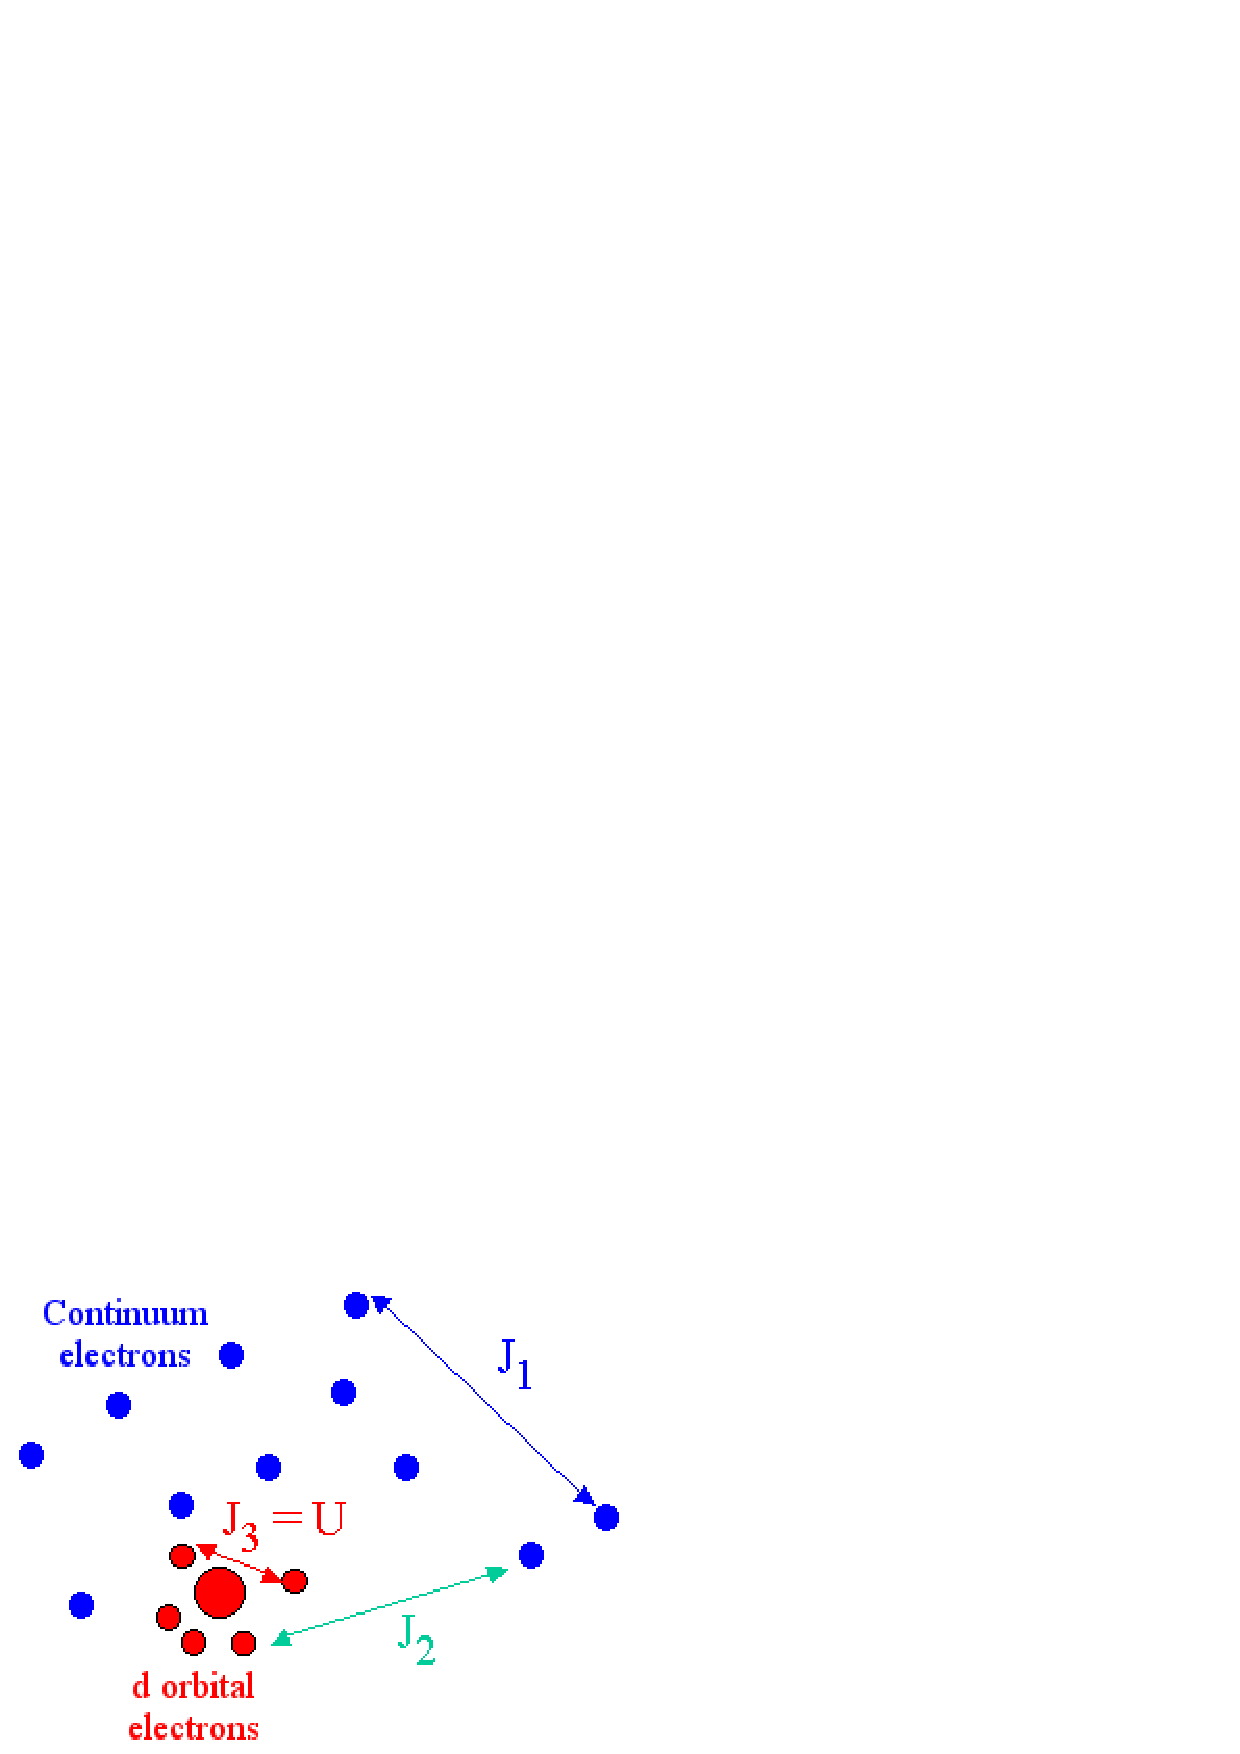
\includegraphics[width=6cm]{01-QD/Pictures/ExchInt.png}
	\end{center}}
	\end{figure}

	Let's begin with the interaction noted $J_1$ on the diagram, two states belonging to the continuum of the semiconductors. This is the hamiltonian $H_{eh}$ introduced in Sec.~\ref{ehExch}.

	
	The next interaction we consider is the one of two electrons from a localized atom. It represents internal transitions of the atom, given by the Hund rule. It is written:
	\begin{align}
		{\cal H}_U = \sum_{d, S, S'} U a_{d, S}^{\dagger} a_{d, S'}^{\dagger} a_{d, S'} a_{d, S'}
	\end{align}
with $U = \int \mathrm{d}\mathbf{r} \mathrm{d}\mathbf{r'} \dfrac{e^2}{4\pi\varepsilon_0 |\mathbf{r} - \mathbf{r'}|} |\Phi_d (\mathbf{r})|^2 |\Phi_d (\mathbf{r'})|^2$ the Coulomb interaction between two electrons on the same orbital with different spins. Thus, it costs more energy to add an electron on the same orbital than on another. The Hund rule is verified, with electrons first filling all orbitals with parallel spin before adding an electron to an orbital with second one, with opposed spin.
	
	The third interaction is the one between an electron from the magnetic atom and an electron from the semiconductor. In the same way as with carriers of the bulk, it can be separated in two terms that will be developed in the next paragraphs: a direct Coulomb interaction between the two electrons, and an exchange interaction arising from the fermionic nature of electrons.
	
	The direct Coulomb interaction can be written:
	\begin{align}
		K &= + \sum_{\mathbf{k}, \sigma, \sigma'} K_{\mathbf{k}} a_{\mathbf{k}, \sigma}^{\dagger} a_{d, \sigma'}^{\dagger} a_{d, \sigma'} a_{\mathbf{k}, \sigma} \\
		\text{with} \nonumber \\
		K_k &= \int \mathrm{d} \mathbf{r} \mathrm{d} \mathbf{r}' |\psi_k (\mathbf{r})|^2 \frac{e^2}{4\pi \varepsilon_0 |\mathbf{r}' - \mathbf{r}|} |\Phi_d (\mathbf{r}')|^2 \nonumber
	\end{align}
It is clear that the spin $\sigma$ (resp. $\sigma'$) of the $\mathbf{k}$ electron (resp. $d$ electron) are not involved in this interaction: they are not changed by it. The wave vector $\mathbf{k}$ is also not affected by this interaction. The direct Coulomb interaction therefore only acts on the total energy of the system. The origin of the energy axis can be redefine to ignore it.

	The second term, the exchange interaction, written in second quantification, reads:
		\begin{align}
			J &= + \sum_{k, k', \sigma, \sigma'} I_{kk'}^{ex} a_{k', \sigma}^{\dagger} a_{d, \sigma'}^{\dagger} a_{k, \sigma'} a_{d, \sigma} = - \sum_{k, k', \sigma, \sigma'} I_{kk'}^{ex} a_{k', \sigma}^{\dagger} a_{k, \sigma'} a_{d, \sigma'}^{\dagger} a_{d, \sigma} \label{sdSQ} \\
			\text{with} \nonumber \\
			I_{kk'}^{ex} &= \int \mathrm{d} \mathbf{r} \mathrm{d} \mathbf{r}' \psi_{k'}^* (\mathbf{r}) \psi_{k}^* (\mathbf{r}') \frac{e^2}{4\pi \varepsilon_0 |\mathbf{r}' - \mathbf{r}|} \Phi_{d}^* (\mathbf{r}) \Phi_{d}^* (\mathbf{r}') \label{sdConst}
		\end{align}
As can be seen on Eq.~\ref{sdSQ}, this interaction exchange the spin $\sigma$ and $\sigma'$ of both electrons, as suggested by its name. Eq.~\ref{sdConst} shows that the spin interaction comes from a Coulomb interaction between two fermions.

	We define:
		\begin{align}
			\begin{array}{l}
				\sigma_{kk'}^z = a_{k, \sigma}^{\dagger} a_{k', \sigma} - a_{k, -\sigma}^{\dagger} a_{k', -\sigma} \\
				\sigma_{kk'}^+ = a_{k, \sigma}^{\dagger} a_{k', -\sigma} \\
				\sigma_{kk'}^- = a_{k, -\sigma}^{\dagger} a_{k', \sigma}
			\end{array}
		\end{align}
Considering now that this interaction does not change the number of electrons on the $d$ orbital of the considered magnetic atom, we can write the interaction as a Kondo hamiltonian~\cite{KacmanD0alphabetaIIVI}:
	\begin{align}
		\label{Exchsd}
		{\cal H}_{sd} = - \sum_{k, k'} I_{kk'}^{ex} \bm{\upsigma}_{k,k'}.\mathbf{S}
	\end{align}
Since $I_{k,k'}^{ex}$ is positive, the negative sign in front of the Kondo hamiltonian shows that the energy minimum is reached when the spins of both electrons are aligned, and is therefore ferromagnetic.
	
	We can now write the total hamiltonian \ref{HamilSQ}, breaking the hamiltonian ${\cal H}_{Coulomb}$ into its different part:
		\begin{align}
			{\cal H}_{SQ} &= {\cal H}_0 + {\cal H}_d + {\cal H}_{hyb} + {\cal H}_{eh} + {\cal H}_{U} + {\cal H}_{sd}
		\end{align}
		
		\subsubsection*{Orbital hybridization}

	We now have two hamiltonians to model the exchange interaction between the impurity and the semiconductor electrons: ${\cal H}_{sd}$ and ${\cal H}_{hyb}$. The first one was put in Heisenberg form in the previous section. This section will focus on the hybridization. The hybridization constant can be written as~\cite{AndersonHamil}:
	\begin{align}
	\label{Vkd}
		V_{kd} = \frac{1}{\sqrt{N}}\int \mathrm{d}\mathbf{r} \Phi_d^* (\mathbf{r} - \mathbf{R_d}) {\cal H}_{HF} (\mathbf{r}) \psi_k (\mathbf{r})
	\end{align}
with $N$ the number of primitive cell in the crystal and ${\cal H}_{HF} (\mathbf{r})$ the Hartree-Fock hamiltonian for a single electron.
	
	Schrieffer and Wolff rewrote the Anderson hamiltonian ${\cal H}_{hyb}$ in order to give a form closer to the Kondo hamiltonian~\cite{RelationAnderKondo}:
	\begin{align}
	\label{Ikk'}
			{\cal H}_{hyb} &= \sum_{k,k'} V_{kd} V_{k'd} \left(\dfrac{1}{E_k - (E_d + U)} + \dfrac{1}{E_{k'} - (E_d + U)}\right. \nonumber \\
			 				& \qquad \qquad \qquad \qquad \qquad \qquad \left. - \dfrac{1}{E_k - E_d} - \dfrac{1}{E_{k'} - E_d}\right)a_{k', \sigma}^{\dagger} a_{k, -\sigma} a_{d, S-2\sigma}^{\dagger} a_{d, S} \nonumber \\
			 				&= -  \sum_{k,k'} I_{kk'}^{hyb} a_{k', \sigma}^{\dagger} a_{k, -\sigma} a_{d, S-2\sigma}^{\dagger} a_{d, S}
	\end{align}
This form suppose that the magnetic atom $d$ levels are far from the band edge. This assumption works well for Mn. However, the Cr ground state is at the edge of the valence band. Therefore, knowing the sign of $E_k - E_d$ or $E_{k'} - E_d$ is more difficult. In order to give an idea of the construction of the hybridization, we will focus on the Mn case. The case of the Cr will be discussed more in details in Sec.~\ref{CrCdTe}.

	\begin{figure}[h!]
	\fcapside{\caption{Schema of the band structure and virtual transitions between valence band and conduction band. Picture taken from Laurent Maingault's PhD thesis~\cite{LaurentTh}. $E_d$ is the ground energy of the $d$ electrons of the magnetic atom; $U$ is the energy needed for the magnetic atom to reach its first excited state; $E_v (k)$ is the valence band energy; $E_g (k)$ is the conduction band energy}\label{EnerTransit}}
	{\begin{center}
		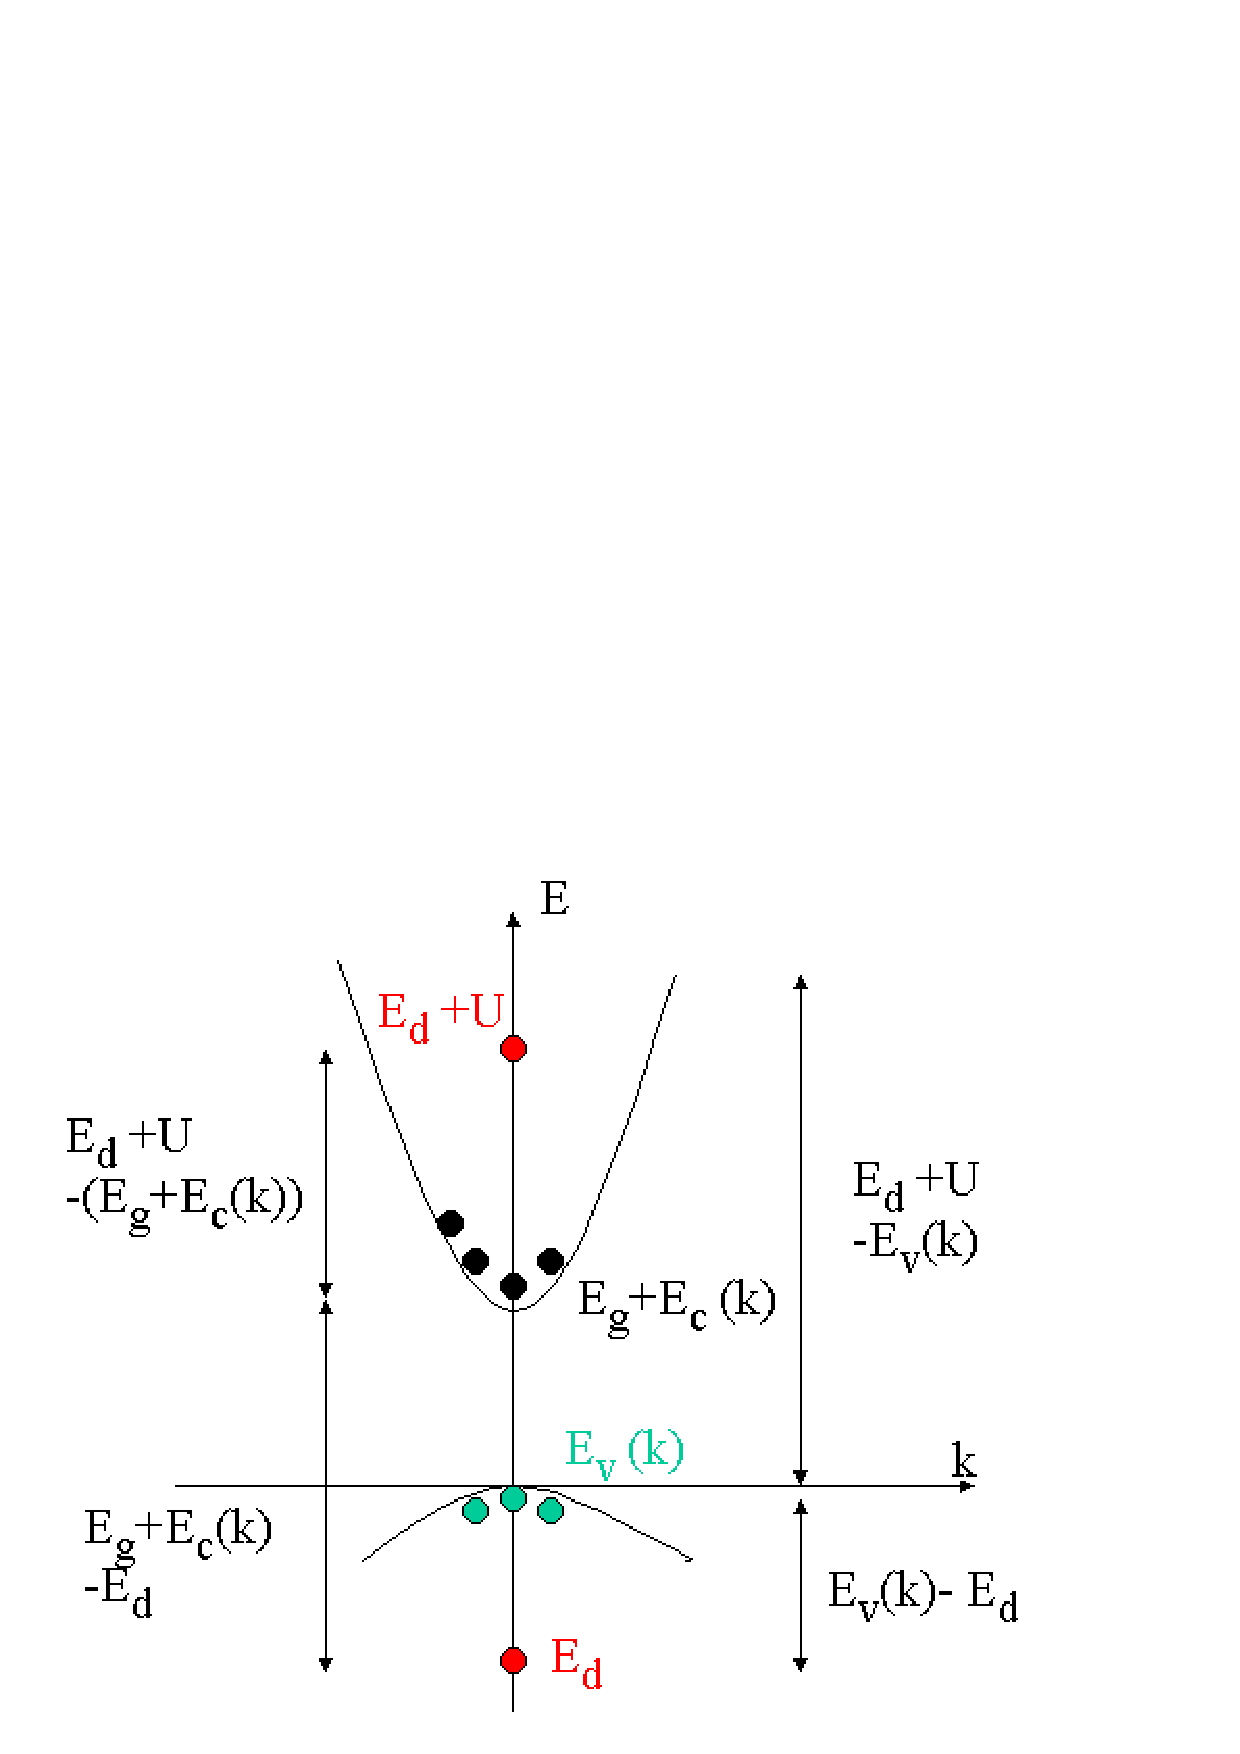
\includegraphics[width=7.6cm]{01-QD/Pictures/EnergyLevels.png}
	\end{center}}
	\end{figure}
	
	The Fig.~\ref{EnerTransit} illustrates the different energies introduced in \ref{Ikk'}, presenting virtual transitions to the $d$ orbital of the magnetic atom. The two possible energies are $E_d$ for the low energy level, and $E_d + U$ for the high energy one, $U$ being the energy needed to add an electron to the orbital.

	Supposing the coupling occurs between two electrons with a close $k$ ($k \simeq k'$), we can rewrite $I_{kk'}^{hyb}$ as:
	\begin{align}
		\begin{array}{rl}
			I_{kk'}^{hyb} &= 2|V_{kd}|^2 \dfrac{U}{(E_k - E_d)(E_k - (E_d + U)} \\
						&= -2|V_{kd}|^2 \dfrac{U}{(E_k - E_d)(E_d + U - E_k)}
		\end{array}
	\end{align}
For a magnetic atom ground state is deep inside the valence band, as it is the case for the Mn atom, $U$ and $E_k - E_d$ are both positive, while $E_k - (E_d + U)$ is negative (see Fig.~\ref{EnerTransit}). Thus, $I_{kk'}^{hyb}$ is negative, and leads to an anti-ferromagnetic one.

\subsubsection*{Exchange constants in DMS}

	With this last transformation, it is now possible to use a Heisenberg type spin hamiltonian for all interactions instead of a hamiltonian mixing wave functions. The only difference between the interactions is in the exchange constant:  $I_{kk'}^{ex}$ for the exchange, and $I_{kk'}^{hyb}$ for the hybridization.

	Using the same hypothesis done on Sec.~\ref{BandStruct} of small $k$ value, and the value of $V_{kd}$ presented in Eq.~\ref{Vkd}, we can rewrite the exchange constant:
	\begin{align}
		I_{00, \{c,v\}}^{hyb} &= -2 \left(\frac{U}{(E_{\{c,v\}}(0) - E_d)(E_d + U - E_{\{c,v\}}(0))}\right) |V_{kd}|^2 \\
		I_{00, \{c,v\}}^{ex} &= \int \mathrm{d}\mathbf{r} \mathrm{d}\mathbf{r}' \psi_0^{*\{c,v\}} (\mathbf{r}) \Psi_d^* (\mathbf{r}) \frac{e^2}{4\pi \varepsilon_0 |\mathbf{r}' - \mathbf{r}|} \psi_0^{\{c,v\}} (\mathbf{r}) \Psi_d (\mathbf{r})
	\end{align}
	
	In the conduction band, the orbitals are $s$, and so we will write the interaction $I_{sd}$. However, since $s$ orbitals have a spherical symmetry, there is no hybridization contribution~\cite{BhattacharjeeExchVB}. The expression is then pretty easy:
	\begin{align}
		I_{sd} = I_{00, c}^{ex}
	\end{align}
As discussed earlier, this lead to a ferromagnetic coupling between the conduction band electrons and the magnetic atom.

	This model can also be used in the valence band~\cite{BhattacharjeeExchVB}. The valence band is formed by the $p$ orbital of the semiconductor matrix, as discussed in Sec.~\ref{BandStruct}. We then write $I_{pd}$ as the sum of the hybridization and the exchange contributions:
	\begin{align}
		I_{pd} =I_{00, v}^{hyb} +  I_{00, v}^{ex}
	\end{align}
The two interactions are in competition in the valence band, with the exchange interaction inducing a ferromagnetic coupling, and the hybridization inducing an anti-ferromagnetic one. The final sign of the interaction depends on the material, and is more discussed in Sec.~\ref{AtinCdTe}.

	The exchange interaction in the valence band can be rewritten for holes, using the total angular momentum $\mathbf{J}$ instead of the pure spin $\mathbf{S}$. However, since $J = 3/2$ and the exchange constant $I_{pd}$ has been defined for $S = 1/2$, the hole exchange hamiltonian have to be written using $I_{pd}/3$.
	
	The interaction between semiconductors carriers one magnetic atom in the Heisenberg notation:
	\begin{align}
	\label{HSingleAt}
	\renewcommand{\arraystretch}{1}
		\begin{array}{rlcccccc}
			{\cal H}_{SQ} &= {\cal H}_0 &+& {\cal H}_{eh} &-& \underbrace{I_{sd} \bm{\upsigma}.\mathbf{S}} &-& \underbrace{\dfrac{I_{pd}}{3} \mathbf{J}.\mathbf{S}} \\
						&= {\cal H}_0 &+& {\cal H}_{eh} &+& {\cal H}_{sd} &+& {\cal H}_{pd}
		\end{array}
	\end{align}
Since a DMS contain a small percentage of magnetic atoms, we can write the hamiltonian of the full semiconductor by summing up the interaction all the sites with magnetic atoms. We finally get:
	\begin{align}
	\label{HDMS}
		{\cal H}_{DMS} &= {\cal H}_0 + {\cal H}_{eh} - \sum_i I_{sd} (\mathbf{R}_i) \bm{\upsigma}.\mathbf{S}_i - \sum_i I_{pd} (\mathbf{R}_i) \mathbf{J}.\mathbf{S}_i
	\end{align}

	This can be further simplified with two approximations. First, since a conduction electron sees a lot of different atomic sites, we can work with the mean value of the magnetic atoms spins, $\langle\mathbf{S} \rangle$, instead of their individual value $\mathbf{S}_i$. This is the mean field approximation, the magnetic atoms being seen as an effective magnetic field. And for the same reason, we can consider the electron interaction with each site of the crystal multiplied by the probability $x$ of being occupied by a magnetic atom, instead of summing only on the magnetic atoms positions. This is the virtual crystal approximation. We can then rewrite:
	\begin{align}
		\sum_i I_{sd} (\mathbf{R}_i) \bm{\upsigma}.\mathbf{S}_i = x \sum_{\mathbf{R}} I_{sd} (\mathbf{R}) \bm{\upsigma}.\langle \mathbf{S} \rangle
	\end{align}
Projecting along the quantization axis, we just replace $\bm{\upsigma}.\langle\mathbf{S} \rangle$ by $\sigma_z \langle S_z \rangle$. Since the atoms are seen as a magnetic field, they induce a degeneracy lift $\Delta E_c$ between the two spin values of conduction electron, $|\sigma_z = \pm \dfrac{1}{2} \rangle$:
	\begin{align}
		\Delta E_c = -N_0 x \alpha \sigma_z \langle S_z \rangle
	\end{align}
with $\alpha \propto I_{sd}^{00}$ the interaction constant between the impurity's and the conduction band's Bloch function at $\mathbf{k} = 0$, and $N_0$ the number of cell per volume.
	
	The same consideration can be done for valence band. It can be written for heavy holes:
	\begin{align}
		\Delta E_v = -N_0 x \frac{\beta}{3} J_z \langle S_z \rangle
	\end{align}
with $\beta \propto I_{pd}^{00}$ the interaction constant between impurity's and the valence band's Bloch function at $\mathbf{k} = 0$.

		\subsubsection*{Interactions for $k \neq 0$}

	To be complete with the analysis, we should also take into account the confinement due to the quantum dot. This means the wave vector $\mathbf{k}$ of the carriers can be different from 0, leading to small perturbative effect on ${\cal H}_{sd}$ and ${\cal H}_{pd}$. This was done in details by Laurent Maingault in the Chap.~I.3 of his PhD thesis~\cite{LaurentTh}. It is shown that the hamiltonian changed as follow:
	\begin{align}
			{\cal H}_{sd} (\mathbf{R}) &= -\alpha \bm{\upsigma}.\mathbf{S} \left| F_c(\mathbf{R}) - A_2\left( \frac{\partial^2 F_c}{\partial z^2} (\mathbf{R}) + \frac{\partial^2 F_c}{\partial \rho^2}(\mathbf{R})\right) \right|^2 \nonumber \\
										&  \qquad \qquad \qquad - \beta \bm{\upsigma}.\mathbf{S} \left( (C_2 - B_2) \left| \frac{\partial^2 F_c}{\partial z^2} (\mathbf{R}) \right|^2 + C_2 \left| \frac{\partial^2 F_c}{\partial \rho^2} (\mathbf{R}) \right|^2 \right) \\
			{\cal H}_{pd} (\mathbf{R}) &= -\beta \mathbf{J}.\mathbf{S} |F_v(\mathbf{R}) - V_{kd} F_v''(\mathbf{R})|^2
	\end{align}
with $F_c(\mathbf{R})$ (resp. $F_v(\mathbf{R})$) the electron (resp. hole) envelop function, $F_v'' (\mathbf{R})$ the second derivative of the hole envelop function, and $A_2$, $B_2$, $C_2$ constant depending on the semiconductor lattice. For CdTe, $A_2 = 10.3$ \AA$^{-2}$, $B_2 = 0.781$ \AA$^{-2}$ and $C_2 = 19.8$ \AA$^{-2}$.

		\subsection{Insertion of Mn or Cr atom in a semiconductor lattice\label{AtinCdTe}}
		
		We will consider in the section the interaction between single magnetic atoms and the carrier trapped in quantum dots. Specifically, we will be interested in the interaction with a Manganese or a Chromium atom. This does not change significantly the picture we drew in the previous section. However, for the interaction between the semiconductor electrons and the magnetic atom $d$ electrons, we will have to also take into account the overlap between the magnetic atom and the carriers. For a magnetic atom A at the position $\mathbf{R}$, we define the exchange constant:
		\begin{align}
			I_{eA} &= - \alpha |F_c (\mathbf{R})|^2 \label{eAexch}\\
			I_{hA} &= - \frac{\beta}{3} |F_v (\mathbf{R})|^2 \label{hAexch}
		\end{align}
			
			\subsubsection*{Mn in CdTe\label{MnCdTe}}
		
		Mn has an electronic structure [Ar]3d$^5$4s$^2$. When inserted into CdTe, it substitutes a Cd atom ([Kr]4d$^{10}$5s$^2$). Both atoms are isolectronics and thus, as Cd, Mn bonds with the neighbouring Te atoms with its two $s$ electrons of its outer shell. In the semiconductor matrix, it is then Mn$^{2+}$ that has to be considered, with an electronic structure [Ar]3d$^5$. Since the $d$ orbital is five time degenerated (doubled when taking spin into account), it is half-full in the case of the Mn. Following Hund's rule, the spin of those electron are all aligned, leading to a total electronic spin $S_{Mn} = 5/2$ and a total orbital momentum $L = 0$.	
		
		Using the exchange constant defined in Eq.~\ref{eAexch} and \ref{hAexch}, we can rewrite the hamiltonian \ref{HSingleAt}:
		\begin{align}
		\label{HSingleMn}
			\begin{array}{rlccc}
				{\cal H}_{cMn} &=& {\cal H}_{eMn} &+& {\cal H}_{hMn} \\
								&=& I_{eMn} \bm{\upsigma}.\mathbf{S}_{Mn} &+& I_{hMn} \mathbf{J}.\mathbf{S}_{Mn}
			\end{array}
		\end{align}
We ignore ${\cal H}_0$ here since it only shift the energy of the system without affecting the spins exchange interactions. We can then write its spin operator as we did for the carriers in Sec.~\ref{BandStruct}:
	\begin{align}
		\begin{array}{rl}
			S_{Mn, x} &= \begin{pmatrix}
						0 & \frac{\sqrt{5}}{2} & 0 & 0 & 0 & 0 \\
						\frac{\sqrt{5}}{2} & 0 & \sqrt{2} & 0 & 0 & 0 \\
						0 & \sqrt{2} & 0 & \frac{3}{2} & 0 & 0 \\
						0 & 0 & \frac{3}{2} & 0 & \sqrt{2} & 0 \\
						0 & 0 & 0 & \sqrt{2} & 0 & \frac{\sqrt{5}}{2} \\
						0 & 0 & 0 & 0 & \frac{\sqrt{5}}{2} & 0
			  		\end{pmatrix} \\
			\\
			S_{Mn, y} &= \begin{pmatrix}
						0 & -\frac{i\sqrt{5}}{2} & 0 & 0 & 0 & 0 \\
						\frac{\sqrt{5}}{2} & 0 & -i\sqrt{2} & 0 & 0 & 0 \\
						0 & \sqrt{2} & 0 & -\frac{3i}{2} & 0 & 0 \\
						0 & 0 & \frac{3}{2} & 0 & -i\sqrt{2} & 0 \\
						0 & 0 & 0 & \sqrt{2} & 0 & -\frac{i\sqrt{5}}{2} \\
						0 & 0 & 0 & 0 & \frac{\sqrt{5}}{2} & 0
			  		\end{pmatrix} \\
			\\
			S_{Mn, z} &= \begin{pmatrix}
						\frac{5}{2} & 0 & 0 & 0 & 0 & 0 \\
						0 & \frac{3}{2} & 0 & 0 & 0 & 0 \\
						0 & 0 & \frac{1}{2} & 0 & 0 & 0 \\
						0 & 0 & 0 & -\frac{1}{2} & 0 & 0 \\
						0 & 0 & 0 & 0 & -\frac{3}{2} & 0 \\
						0 & 0 & 0 & 0 & 0 & -\frac{5}{2}
				   \end{pmatrix}
		\end{array}
	\end{align}

		In the conduction band, the electrons $s$ orbitals are orthogonal to the $d$ orbital of the Mn atom. No hybridization can then occur. Only the Coulomd interaction remain, leading to a standard ferromagnetic interaction between conduction band electrons and Mn electronic spin. Confirming this, $N_0 \alpha = 0.22 \pm 0.01$ eV was measured~\cite{GajMnD0alphabeta}.
		
		The deduction is a bit harder to work out in the valence band. Valence electrons $p$ orbitals are not orthogonal to Mn electrons $d$ orbital, meaning there is a competition between the standard ferromagnetic exchange interaction and the $pd$ hybridization. It turns out that the hybridization is stronger than Coulomb exchange interaction for Mn in II-VI semiconductor, leading to an anti-ferromagnetic interaction between holes and Mn electronic spin~\cite{KacmanD0alphabetaIIVI}. For Cd$_x$Mn$_{1-x}$Te, $N_0 \beta = -0.88 \pm 0.01$ eV was measured, confirming this anti-ferromagnetism of the interaction.~\cite{GajMnD0alphabeta}.

	
			\subsubsection*{Cr in CdTe\label{CrCdTe}}
		Cr as an electronic structure [Ar]3d$^4$4s$^2$. Cr is also iso-electronic with the Cd and thus is introduced in the lattice in substitution to this atom, bonding with its two $s$ electrons and thus being inserted as [Ar]3d$^4$. Following Hunds rule for the Cr $d$ orbital, with find that Cr in CdTe has a total electronic spin $S_{Cr} = 2$ and a total orbital momentum $L=2$.
		
		As done with the Mn, we can rewrite the hamiltonian~\ref{HSingleAt} using the exchange interaction defined in the introduction of this section:
		\begin{align}
		\label{HCrDMS}
			\begin{array}{rlccc}
				{\cal H}_{cCr} &=& {\cal H}_{eCr} &+& {\cal H}_{hCr} \\
									&=& I_{eCr} \bm{\upsigma}.\mathbf{S}_{Cr} &+& I_{hCr} \mathbf{J}.\mathbf{S}_{Cr}
			\end{array}						
		\end{align}
Once again, we ignore ${\cal H}_0$ since it did not affect the spins exchange interaction. We can also write the Cr spin operators as follows:
	\begin{align}
		\begin{array}{rl}
			S_{Cr, x} =& \begin{pmatrix}
					0 & 1 & 0 & 0 & 0 \\
					1 & 0 & \sqrt{\frac{3}{2}} & 0 & 0 \\
					0 & \sqrt{\frac{3}{2}} & 0 & \sqrt{\frac{3}{2}} & 0 \\
					0 & 0 & \sqrt{\frac{3}{2}} & 0 & 1 \\
					0 & 0 & 0 & 1 & 0
				   \end{pmatrix} \\
			\\
			S_{Cr, y} = i&
				   \begin{pmatrix}
					0 & -1 & 0 & 0 & 0 \\
					1 & 0 & -\sqrt{\frac{3}{2}} & 0 & 0 \\
					0 & \sqrt{\frac{3}{2}} & 0 & -\sqrt{\frac{3}{2}} & 0 \\
					0 & 0 & \sqrt{\frac{3}{2}} & 0 & -1 \\
					0 & 0 & 0 & 1 & 0
				   \end{pmatrix} \\
			\\
			S_{Cr, z} =& \begin{pmatrix}
					2 & 0 & 0 & 0 & 0 \\
					0 & 1 & 0 & 0 & 0 \\
					0 & 0 & 0 & 0 & 0 \\
					0 & 0 & 0 & -1 & 0 \\
					0 & 0 & 0 & 0 & -2
				   \end{pmatrix}
		\end{array}
	\end{align}
		
		In the conduction band, the situation is the same as with Mn: the conduction electrons $s$ orbital are orthogonal to the Chromium $d$ orbital, and the hybridization is then zero. Only the Coulomb interaction remains and induces a ferromagnetic coupling between the electrons of the band and the Cr electronic spin. $N_0 \alpha$ was never measured in Cd$_x$Cr$_{1-x}$Te, but most magnetic atoms in II-VI semiconductor presents a value between $0.2$ eV and $0.3$ eV. It is then generally assumed that, in II-VI semiconductor, $N_0 \alpha \approx 0.2$ eV~\cite{MacspdexchCr}. We also chose to use this value.
		
		%Once again, valence band is a bit 
		In the valence band, the picture for Cr in CdTe is a lot more complicated and still open to discussions. The position of the $d$ ground state energy relative to the semiconductor valence band is critical and can make the kinetic exchange interaction change sign (see Fig.~\ref{EnerTransit} and Eq.~\ref{Ikk'} for a $d$ level energy $E_d$ in the gap). Cr 3$d$ level is almost at the same energy as the top of CdTe valence band, making it hard to decide whether it is in the gap or not.
		%It was however predicted that the sign of the interaction could change between hh and lh~\cite{WojtowiczXNewDMS}.
		
		$N_0\beta$ was never directly measured in Cd$_x$Cr$_{1-x}$Te and is challenging to find theoritically for the reason stated in the previous paragraph~\cite{BlinowskiFerroCrDMS}. Wojtowicz et al. measured the Zeeman spin splitting of 1$S$ excitons in a quantum well. The results were coherent with an interaction of opposite signs for lh and hh~\cite{WojtowiczXNewDMS}. The evolution suggest a ferromagnetic interaction for hh and antiferromagnetic for lh. $N_0 \beta$ was found positive (ferromagnetic) in Cd$_x$Cr$_{1-x}$S~\cite{MacCdCrSD0beta} and in all the studied Zn based II-VI semiconductors, assuming $N_0 \alpha = 0.2$ eV~\cite{KacmanD0alphabetaIIVI}. Especially, in ZnTe, for $N_0 \alpha = 0.2$, a large ferromagnetic $N_0 \beta = +3.6 \pm 1.2$ eV was found~\cite{MacspdexchCr}. Since there is almost no valence band offset between ZnTe and CdTe and that the transition metal impurity levels does not significantly changes between compounds with common anions~\cite{KossutHandbook}, it could be reasonable to assume that $N_0 \beta$ in bulk CdTe is positive, giving a ferromagnetic hole-Cr interaction. However, any parameter that can change the position of the relative energies of the top of the valence band and of the $d$ orbitals, such as strain or the confinement, can affect the sign of this interaction.


	\section{Fine and hyperfine structure of a magnetic atom in II-VI semiconductors}

		\subsection{Mn atom in II-VI semiconductors~\label{MnSemiCon}}
		

		
	We saw that the Mn $d$ orbital is the outside orbital for Mn in CdTe and is half-filled, with 5 electrons on it. Following Pauli exclusion principle, this gives the Mn atom in a CdTe lattice an angular momentum $L = 0$.

		
		We get from Hund's rule that adding an electron to an half-filled orbital has a high energy cost. The lowest energy excited states are therefore the flipping of an electron. For a free atom, it leads to a first excited state with an angular moment $L = 4$. Following the spectroscopic notation of these states $^{(2S+1)}L$, the ground state is noted $^6$S ($L=0$, $S = \frac{5}{2}$) and the first excited state is $^4$G ($L = 4$, $S = \frac{3}{2}$). Higher energy excited states also exist, but have no influence in our study. We can safely neglect them.
		
	\begin{figure}[h!]
	\begin{center}
		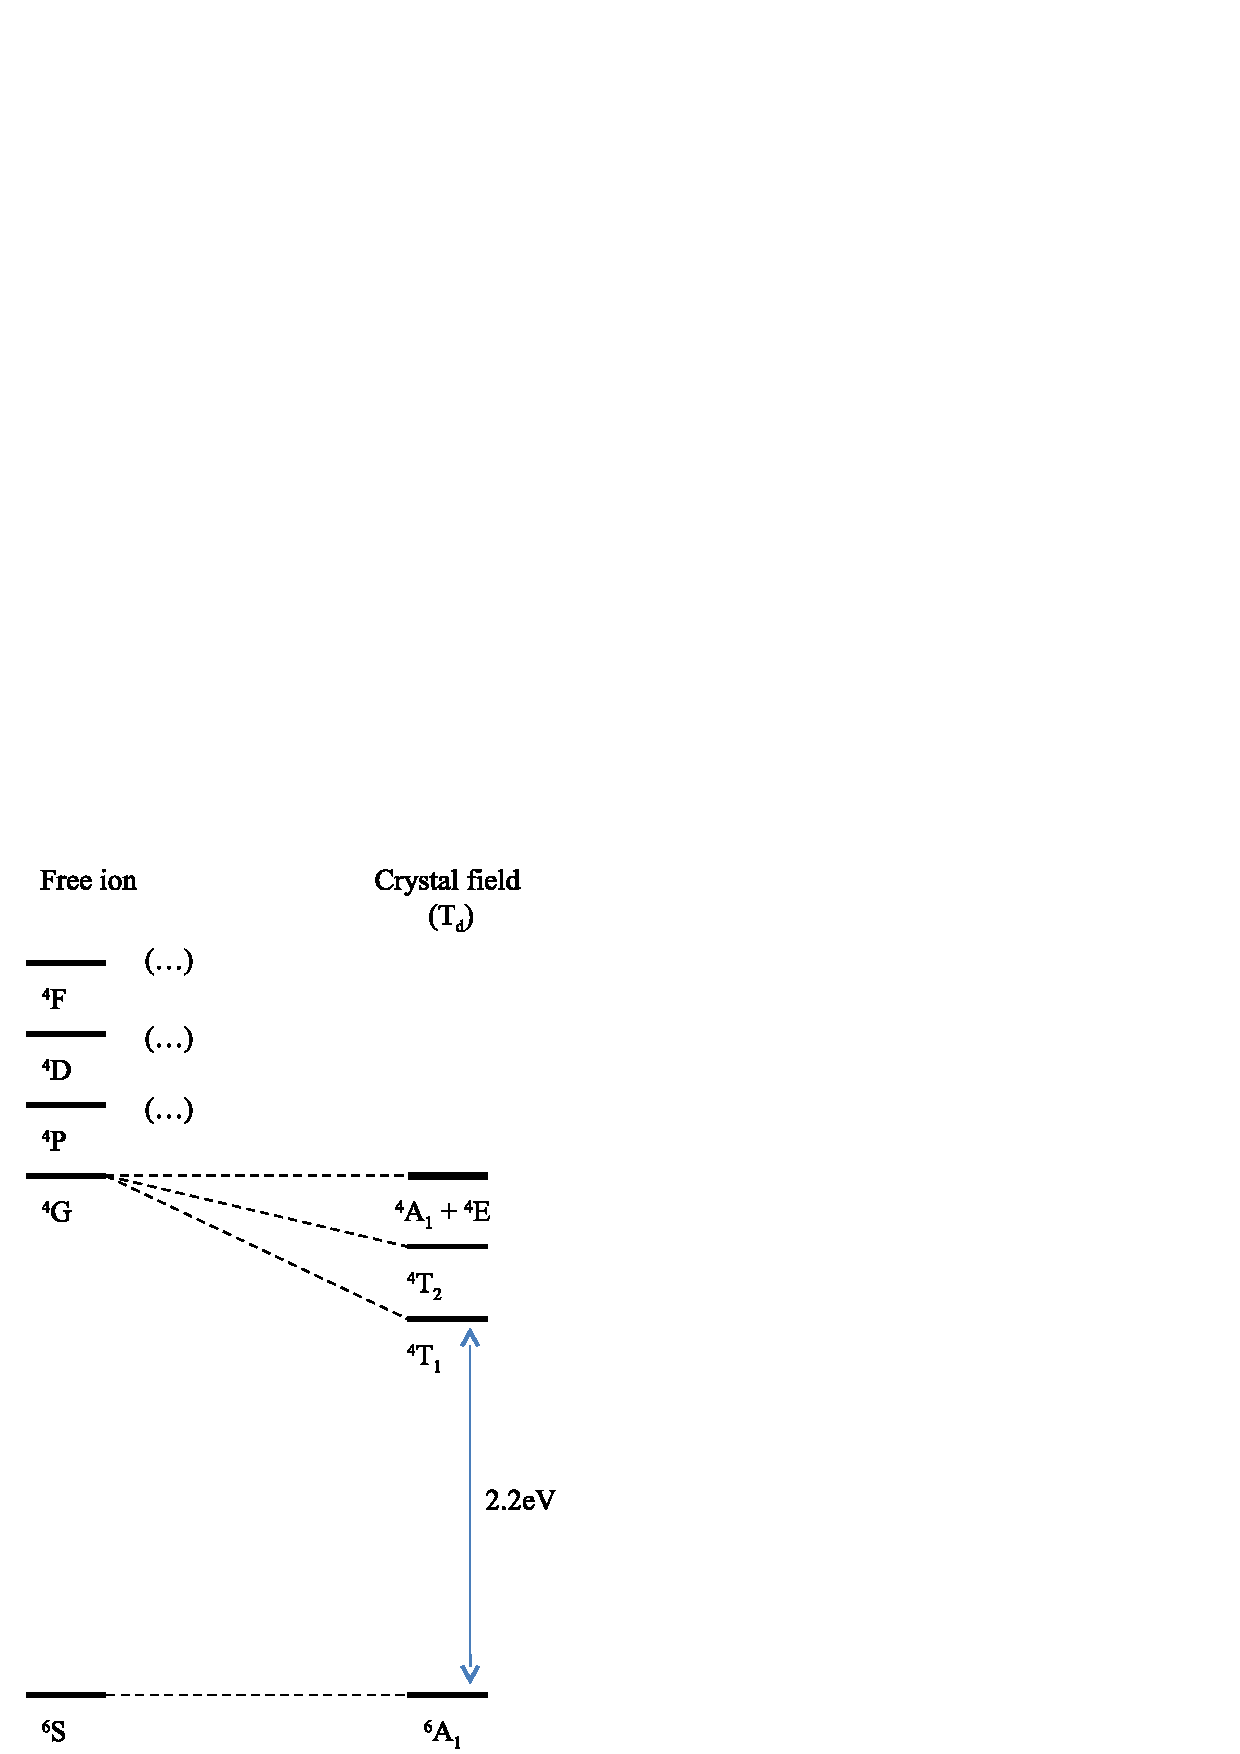
\includegraphics[width=10cm]{01-QD/Pictures/MnCrystal.png}
	\end{center}
	\caption{Schematic diagram of the effect of the crystal field, biaxial strain and spin-orbit coupling on the Mn$^{2+}$ 3$d^5$ ground state ($^6$S). Effect of the crystal field on the first excited state ($^4$G) are also presented.}
	\label{MnCrystal}
	\end{figure}
		
		When inserted in the semiconductor matrix of $T_d$ symmetry, the interaction with the crystal field will lift the degeneracies of the free atom level. Those new levels are written with the appropriate group theoritical transformation properties. The $^6$S ground state is symmetrical and non-degenerated, except for spin. Thus, it is not affected by the crystal field and is noted $^6$A$_1$. On the other hand, $^4$G, the first excited state, has an orbital degeneracy and therefore is affected by the crystal field. It split into four different states: $^4$T$_1$, three-fold degenerated ; $^4$T$_2$, three-fold degenerated ; $^4$E, two-fold degenerated ; and $^4$A$_1$, not degenerated. It has been shown by calculations~\cite{TanabeGroupThMn,SolidStatesPhysics,ThTransMetalIon} that the effect of the crystal field is to pull the two $^4$T levels closer to the ground state, while $^4$E and $^4$A$_1$ are weakly affected by the crystal field.

	For a free atom, the transition between the ground state with $S=\frac{5}{2}$ and any of the excited states, with $S = \frac{3}{2}$ is forbidden by the $\Delta S = 0$ rule and the parity selection ones. However, in a II-VI lattice, the spin-orbit interaction and the absence of inversion symmetry relax those rules. The transitions between $^6$A$_1$ and the different states coming from the $^4$G splitting are allowed. $^6$A$_1 \rightarrow ^4$T$_1$ is the lowest energy of those transitions and therefore the most significant. It corresponds to approximately 2.2 eV. This transition can kill the luminescence of a semiconductor: the electron-hole recombination excite a $d$ electron instead of emitting a photon. However, this transition is unlikely to happen. For high concentration of Mn, it will significantly reduces the photoluminescence of the sample. However, we work at a really low concentration of Mn atoms in order to have QD with only one of them. This phenomena shouldn't then have a noticeable effect on our samples.
	

	$^6$A state of the Mn$^{2+}$ has no orbital degeneracy and thus is not affected by the T$_d$ crystal field nor by the reduction of its symmetry by the biaxial strain.  However, the spin degeneracy is lifted by a combination of spin-orbit interaction and reduced symmetry of the crystal field. In the presence of biaxial strain, this will results in a splitting the spin level according to $D_0S_z^2$~\cite{D0Sz}, with $D_0$ the magnetic anisotropy and $S_z$ the Mn spin quantized along the $z$ axis. Due to the null Mn orbital momentum ($L = 0$), the magnetic anisotropy is however weak and the spin splitting is only of a few tens of $\mu$eV, depending on the strains.
	
	\begin{figure}[h!]
	\begin{center}
		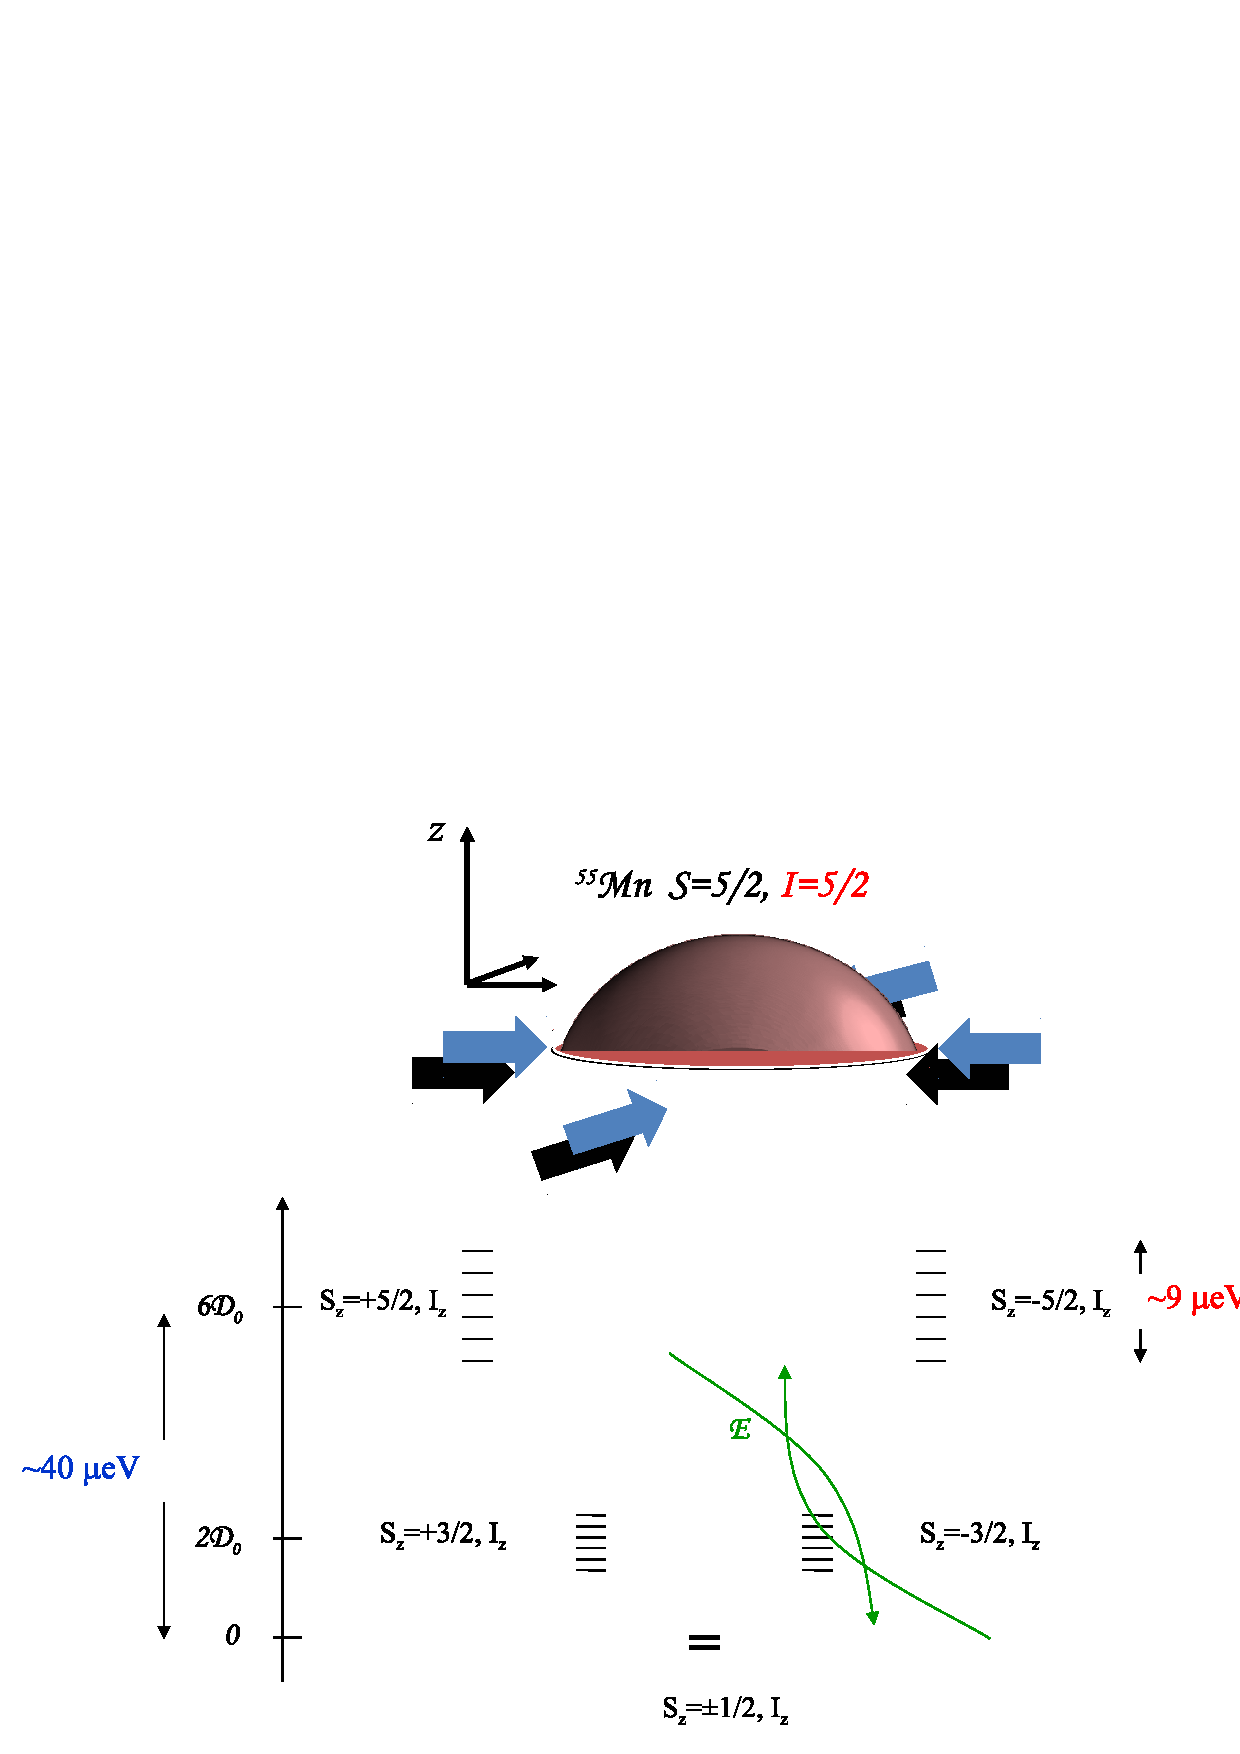
\includegraphics[width=12cm]{01-QD/Pictures/MnFineStruct.png}
	\end{center}
	\caption{Top: schematic view of a strained QD containing a magnetic atom. Bottom: schema of the fine and hyperfine structure of a Mn atom in a strained II-VI QD. The influence of the magnetic anisotropy $D_0$, the in-plane anisotropy $E$ and the hyperfine interaction ${\cal A}$ are represented.}
	\label{MnFineHyperfines}
	\end{figure}
	
	To describe in detail the spin energy levels of a Mn atom, one has also to consider its nuclear spin is $I = \frac{5}{2}$ for all its isotopes. This nuclear spin couples to the $3d$ electrons via the hyperfine interaction. The whole hamiltonian of an electronic spin coupled to the nuclear spin of a Mn atom in a strained layer grow along [001] axis is known from electron paramagnetic resonance in CdTe/ZnTe superlattices~\cite{StrainedMn} and reads:
	\begin{align}
	\label{Mnalone}
		\begin{array}{rll}
			{\cal H}_{Mn} &=& {\cal A}\mathbf{I}.\mathbf{S} \\
							& & +\dfrac{1}{6}a (S_x^4 + S_y^4 + S_z^4 - \dfrac{1}{5}S(S+1)(3S^2+3S-1)) \\
							& & + D_0 (S_z^2 - \dfrac{1}{3}S(S+1)) + E(S_x^2 - S_y^2)
		\end{array}
	\end{align}
	
	The first term is the hyperfine interaction between the Mn nuclear spin $\mathbf{I}$ and its $5d$ electrons spin $\mathbf{S}$, coupling two consecutive Mn spin states through an electron-nuclei flip flop. The hyperfine constant of the Mn was found to be ${\cal A} \approx 0.71$ $\mu$eV~\cite{MnSpinLatticeCoeff}. The second term results from the crystal cubic symmetry and mixes different $S_z$ of the Mn spin. According to ref.~\cite{MnSpinLatticeCoeff}, $a = 0.32$ $\mu$eV.
	
	The last line contains terms linked to the strain state at the Mn position: the magnetic anisotropy caused by bi-axial strain $D_0$ and the anisotropy of strain in the $xy$ plane $E$. Because of the partial relaxation of strain in the self-assembled QD we used, the value of $D_0$ may vary between 0 $\mu$eV for a strain-free QD, to 12 $\mu$eV for a fully strain CdTe layer matched on ZnTe. Typical values around 7 $\mu$eV are usually observed in CdTe/ZnTe QDs~\cite{MnResSpinDyn,GorycaPrecession}, leading to the 40 $\mu$eV splitting presented on Fig.~\ref{MnFineHyperfines}.
	
	An anisotropy of the strain in the QD plane can induce a mixing between different $S_z$ through the anisotropic crystal field parameter $E$. It coupled two values of $S_z$ separated by two units of spin. In the absence of magnetic anisotropy ($D_0 \simeq 0$), both the anisotropy of strain and the hyperfine structure prevent the optical pumping of the Mn spin at zero magnetic field.

		\subsection{Cr atom in II-VI semiconductor\label{CrSemiCon}}
	
		

		Cr atoms are incorporated into II-VI semiconductors as Cr$^{2+}$ ions on cation sites forming a deep impurity level. 90\% of Cr isotopes presents \emph{no nuclear spin}, meaning we do not have to consider their hyperfine structure. The ground state of a free Cr$^{2+}$ is $^{5}$D with the orbital quantum number L=2 and a spin S=2 yielding a 25-fold degeneracy. In the crystal field of T$_{d}$ symmetry of the tetrahedral cation site in zinc-blende crystal, the degeneracy is partially lifted (see Fig.~\ref{CrinIIVI}): the $^{5}$D term splits into 15-fold degenerate orbital triplet $^{5}$T$_{2}$ and 10-fold degenerate orbital doublet $^{5}$E, separated by a gap $\Delta \approx 0.5$ eV. As in the case of Mn, this transition introduce a path for non-radiative recombination and can kill the luminescence of the host semiconductor. We have then to keep the Cr concentration low in order for this transition to not become the main recombination path.
		
	The Jahn-Teller distortion further reduces the symmetry to D$_{2d}$ and leads to a splitting of the $^{5}$T$_{2}$ ground state into a 5-fold degenerate $^{5}$B$_{2}$ orbital singlet and a $^{5}$E orbital doublet .

		The ground state orbital singlet $^{5}$B$_{2}$ is further split by the spin-orbit interaction. In a strain free crystal, it was found that the ground state splitting can be described by the spin effective Hamiltonian~\cite{EPRCr}:
		\begin{align}
			\label{exchange}
			{\cal H}_{Cr,CF}=D_0S_z^2+\frac{1}{180}F[35S_z^2-30S(S+1)S_z^2+25S_z^2]+\frac{1}{6}a[S_1^4+S_2^4+S_3^4]
		\end{align}
with the Cr spin $S=2$ and $|D_0|\gg|a|$, $|F|$. In the following, we will use $a=0$ and $F=0$. The x, y, z principal axes were found to coincide with the cubic axes (1,2,3) giving rise to three identical sites, each given by \ref{exchange} but with the z axis of each along a different cubic axis (1,2,3). A value of $D_0\approx+30$ $\mu$eV was estimated from Electron Paramagnetic Resonance (EPR) measurements in highly diluted bulk (Cd,Cr)Te~\cite{EPRCr}.

		\begin{figure}[hbt]
			\label{CrinIIVI}
			\begin{center}
				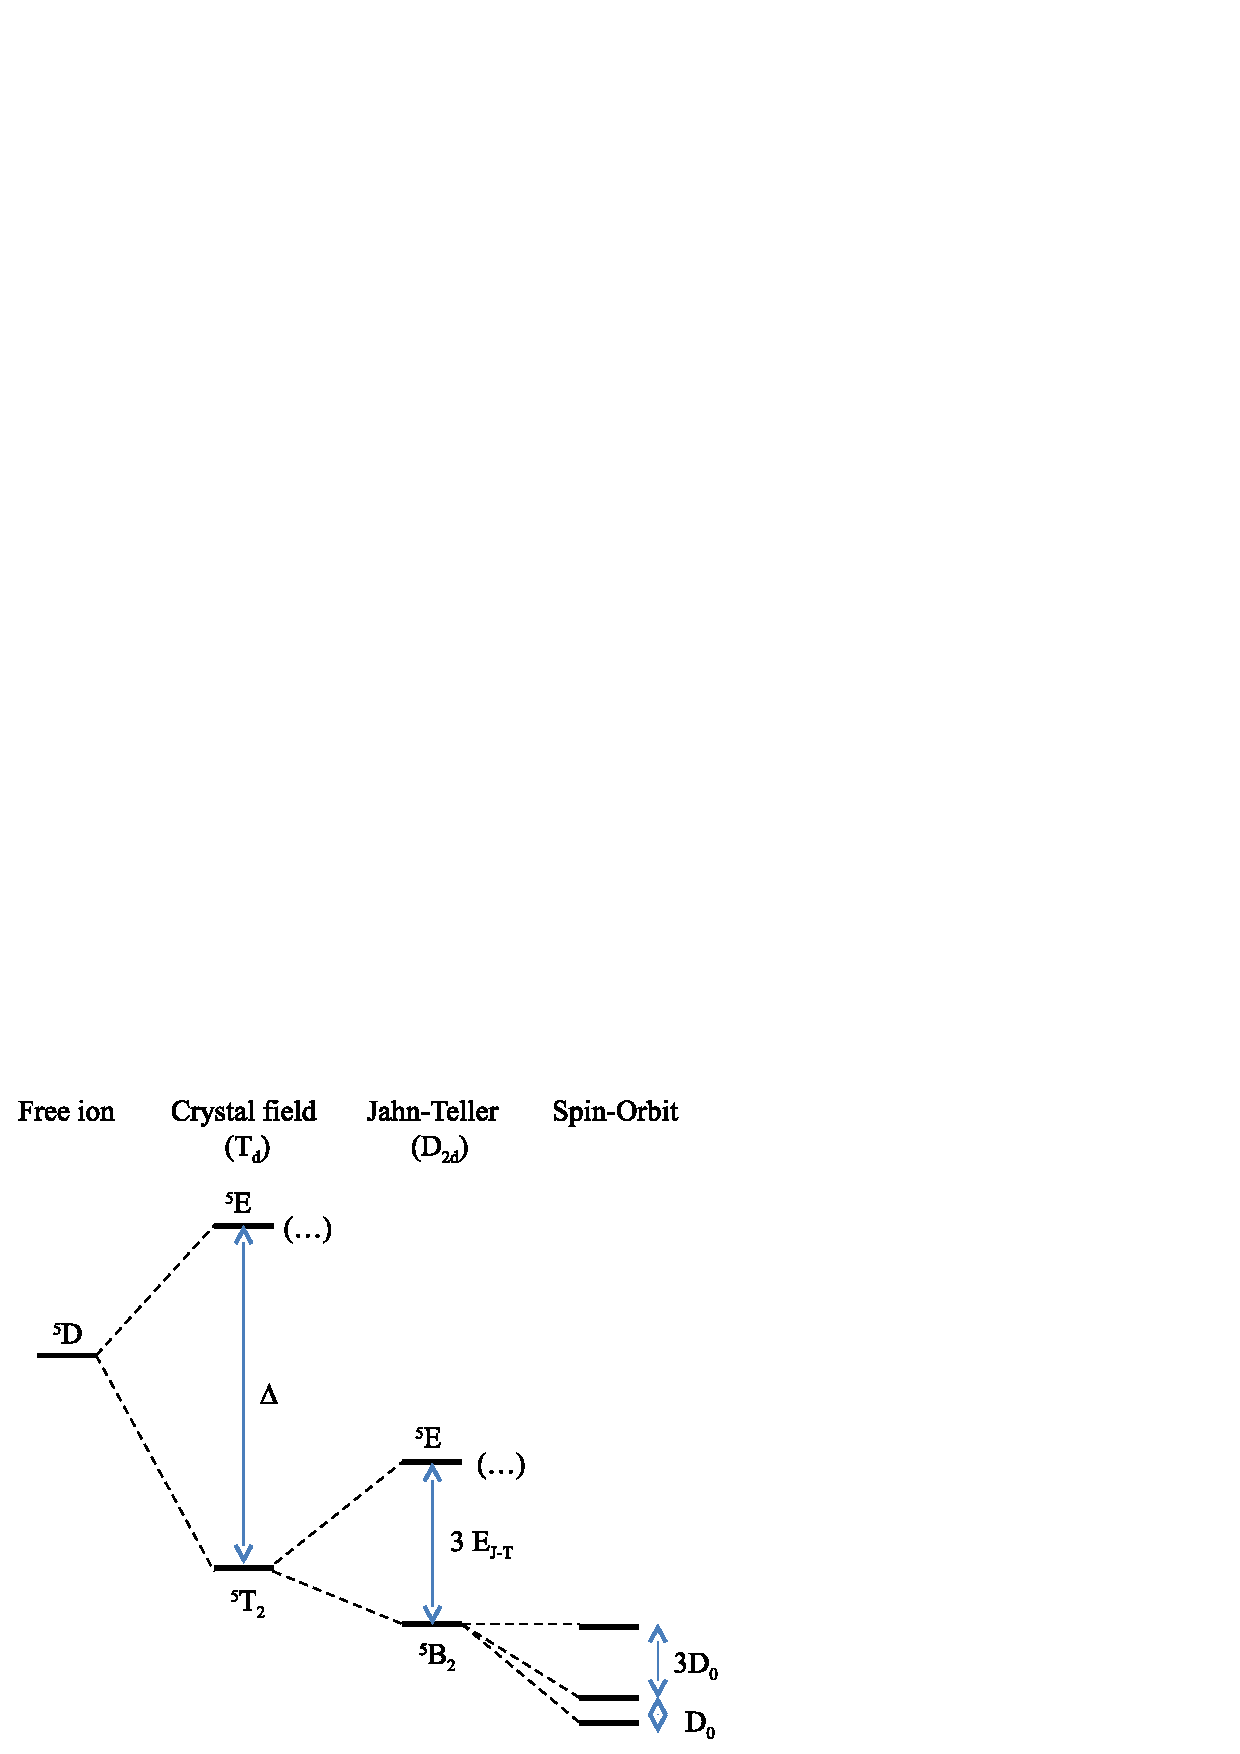
\includegraphics[width=10cm]{01-QD/Pictures/CrinIIVI.png}
			\end{center}
			\caption{Schema of the energy level splitting of Cr$^{2+}$ at a tetragonal site (T$_d$ symmetry) with a crystal field parameter $\Delta$, a Jahn-Teller energy $E_{J-T}$ and a spin-orbit level spacing $D_0$.}
		\end{figure}
		
		Static biaxial compressive strain in the (001) plane, as observed in self-assembled quantum dots, reduces the symmetry to D$_{2d}$ and destabilize the Cr $3d$ orbitals $d_{xz}$ and $d_{yz}$ having an electron density pointing along the $[$001$]$ axis ($z$ axis). The Cr ground state is then a 5-fold degenerated orbital singlet formed from the $d_{xy}$ orbital. It corresponds to the Jahn-Teller ground state with a tetragonal distortion along the $[$001$]$ axis~\cite{DefPonctSemiCon}.

		An applied stress will also  influence the Cr spin fine structure splitting through the modification of the crystal field and the spin-orbit interaction~\cite{EPRCr}. For an arbitrary strain tensor, the general form of the Cr ground state spin effective Hamiltonian is
		\begin{align}
		\label{FullCrHamil}
			{\cal H}_{Cr,\varepsilon} = c_1 e_A S_{\theta} + c_2 e_{\theta} S_{\theta} + c_3 e_{\epsilon} S_{\epsilon} + c_4e_{\zeta} S_{\zeta} + c_5(e_{\xi} S_{\xi} + e_{\eta} S_{\eta})
		\end{align}
with $S_i$ defined as:
		\begin{align}
			\begin{array}{rl}
			\label{Svalues}
				S_{\theta} &= S_{z}^2  -\dfrac{1}{2} [S_{x}^2 + S_{y}^2] \\
				S_{\epsilon} &= \dfrac{1}{2} \sqrt{3} [S_{x}^2 - S_{y}^2] \\
				S_{\xi} &= S_{y} S_{z} + S_{z} S_{y} \\
				S_{\eta} & = S_{x} S_{z} + S_{z} S_{x} \\
				S_{\zeta} &=S_{x} S_{y} + S_{y} S_{x}
			\end{array}
		\end{align}
and $e_i$ defined similarly as:
		\begin{align}
			\begin{array}{rl}
			\label{evalues}
				e_{\theta} &= \varepsilon_{zz} - \dfrac{1}{2} [\varepsilon_{xx} + \varepsilon_{yy}] \\
				e_{\epsilon} &= \dfrac{1}{2} \sqrt{3}[\varepsilon_{xx} - \varepsilon_{yy}] \\
				e_{\xi} &= \varepsilon_{yz} + \varepsilon_{zy} \\
				e_{\eta} &= \varepsilon_{xz} + \varepsilon_{zx} \\
				e_{\zeta} &= \varepsilon_{xy} + \varepsilon_{yx} \\
				e_A &= \varepsilon_{xx} + \varepsilon_{yy} + \varepsilon_{zz}			
			\end{array}
		\end{align}

		As shown in Sec.~\ref{BPSec}, we can write for a flat self-assembled quantum dot with dominant large biaxial strain:
		\begin{align*}
			\varepsilon_{xx} = \varepsilon_{yy} = \varepsilon_{\parallel} \\
			\varepsilon_{zz}=-2\frac{C_{11}}{C_{12}}\varepsilon_{\parallel}
		\end{align*}
where C$_{11}\approx$ 5.4 10$^{10}$ Pa and C$_{12}\approx$ 3.7 10$^{10}$ Pa are the elastic constants of CdTe~\cite{CdTeElConst}. For this strain configuration, the Cr fine structure is controlled by the spin-lattice coupling coefficients $c_1$ (symmetric coefficient) and $c_2$ (tetragonal coefficients). Strain-coupling coefficients estimated from EPR measurements in bulk Cr doped CdTe are listed in table \ref{StrCouplCoef}.

		\begin{table}[htb] \centering
			\caption{Values for spin to strain coupling coefficients of Cr in bulk CdTe (in $meV$) extracted from ref.~\cite{EPRCr}.\label{StrCouplCoef}}
			\renewcommand{\arraystretch}{1.0}
			\begin{tabular}{ccccc}
				\hline\hline
				$c_{1}$ & $c_{2}$ & $c_{3}$  & $c_{4}$  & $c_{5}$ \\
				-0.25$\pm$2 & +4.9 $\pm$2& -1.25$\pm$0.5 & +4.9$\pm$2 & +3.7$\pm$1.25 \\
				\hline\hline
			\end{tabular}
		\end{table}

		We can now simplify the hamiltonian \ref{FullCrHamil}, first reducing it to the active term in our case:
		\begin{align*}
			{\cal H}_{Cr,\varepsilon} &= c_1 e_A S_{\theta} + c_2 e_{\theta} S_{\theta}
		\end{align*}
Replacing now $e_A$, $e_{\theta}$ and $S_{\theta}$ by their value given in \ref{Svalues} and \ref{evalues}, and using the equalities given in Sec.~\ref{BPSec}, we can rewrite the strain controlled part of the spin Hamiltonian as ${\cal H}_{Cr,\varepsilon}$, depending only on $\varepsilon_{\parallel}$:
		\begin{align}
			\begin{array}{rlcc}
			\label{HamilD0}
				{\cal H}_{Cr,\varepsilon_{\parallel}} &=& \underbrace{\dfrac{3}{2}\varepsilon_{\parallel}[2c_1(1-\dfrac{C_{12}}{C_{11}})-c_2(1+2\dfrac{C_{12}}{C_{11}})]} & S_z^2 \\
													&=& D_0 & S_z^2
			\end{array}
		\end{align}
where we can estimate $D_0\approx 1\pm0.6$ meV from the values of the spin-strain coupling coefficients in CdTe (table \ref{StrCouplCoef}). This is about 100 times stronger than the value found in Mn QDs, as stated on Sec.~\ref{MnSemiCon}.
One should note the QDs could be partially relaxed and may contain a significant amount of Zn. This could significantly change the spin-strain coupling coefficients of the Cr atom.

		An anisotropy of the strain in the quantum dot plane (001) with principal axis along $[$010$]$ or $[$100$]$ axes ($\varepsilon_{xx}\neq\varepsilon_{yy}$ and $\varepsilon_{xy} = \varepsilon_{yx}=0$) would affect the Cr fine structure through the tetragonal coefficient $c_3$. This coupling can be described by an additional term in the spin-strain Hamiltonian
		\begin{align}
			\begin{array}{rlcc}
			\label{HamilE}
				{\cal H}_{Cr,\varepsilon_{\perp}} &=& \underbrace{\dfrac{3}{4} c_3 (\varepsilon_{xx}-\varepsilon_{yy})} & (S_x^2 - S_y^2) \\
												&=& E & (S_x^2 - S_y^2)
			\end{array}
		\end{align}

		This anisotropy term $E$ couples Cr spin states separated by two units and in particular $S_z$=+1 to $S_z$=-1 which are initially degenerated. It could be exploited to induce a large strain mediated coherent coupling between a mechanical oscillator and the Cr spin~\cite{SpinOsciCoupl}.
		
		We can now group \ref{HamilD0} and \ref{HamilE} in order to write the complete hamiltonian of an isolated Cr in a CdTe/ZnTe QD with anisotropic strains :
		\begin{align}
			\label{Cralone}
			{\cal H}_{Cr,\varepsilon} = D_0 S_z^2 + E(S_x^2 - S_y^2)
		\end{align}
		
		This large sensitivity of the Cr spin to local strains makes the Cr a particularly interesting qubit for the development of hybrid spin-mechanical systems~\cite{CouplingNVOscill,LafuenteStrainMn,QuantSpinTrasducer}.
	
	
	\section{The X-Mn system\label{XMn}}
	
	In order to illustrate the concepts explained in this chapter, we will present a quick study of a well known system: the exciton coupled to a single Manganese atom. In order to simplify the study, let's consider a QD containing a single Mn atom with no shape or strain anisotropy. When an exciton is injected in the QD, it will interact with the magnetic atom spin in addition to the hole-electron interaction already taking place for an exciton. The hamiltonian of the system reads:
	\begin{align}
		\label{HXMn}
		{\cal H}_{XMn} = {\cal H}_{eh} + {\cal H}_{eMn} + {\cal H}_{hMn}
	\end{align}
We use in this part the heavy-hole approximation, ignoring the effect of the non-diagonal term of the band hamiltonian.

	\begin{figure}[h!]
	\begin{center}
		\includegraphics[width=11cm]{01-QD/Pictures/XMn-Exp.eps}
	\end{center}
	\caption{Photoluminescence of the X, X$^-$ and X$^2$ complex for (a) a QD with no magnetic atom and (b) a QD containing a single Mn atom.}
	\label{MnSpectra}
	\end{figure}

	In the heavy hole subspace, in the $\sigma_z$, $j_z$, $S_z$ basis, all the hamiltonians describing an interaction with the hole are diagonal. Therefore, the only non-diagonal element in the hamiltonian~\ref{HXMn} describe electron-Mn spin-flips. The hole having no part in this interaction, those spin-flips couple a bright state to a dark state, separated by $\delta_0$, as defined in Sec.~\ref{ehExch}. The strength of this interaction is of the same magnitude as $I_{eMn}$, found to be in the 100 $\mu$eV range in our quantum dots~\cite{DynhMn}. Since distance between the bright and dark states is about one order of magnitude higher than the strength of the interaction, we neglect it.
	
	\begin{figure}[h!]
	\begin{center}
		\includegraphics[width=12cm]{01-QD/Pictures/MnEnLvl.png}
	\end{center}
	\caption{Energy level of the ground state and the exciton in a Mn-doped QD. The levels are sketched as a function of the Mn spin $S_z$. Dark states are represented in grey. Optical transitions from the bright states of the Mn complex results in six-line PL spectra, such as in Fig.~\ref{MnSpectra}.}
	\label{MnLevel}
	\end{figure}
	
	We can now consider the hamiltonian~\ref{HXMn} to be diagonal. The interaction of the Mn spin with electron is ferromagnetic with $I_{eMn} \simeq -100$ $\mu$eV, while its interaction with the hole is anti-ferromagnetic with $I_{hMn} \simeq 250$ $\mu$eV.  The carriers act on the Mn spin as an effective magnetic field oriented along the growth axis. This lift the degeneracy of the Mn spins in a sextuplet. For the bright exciton, with anti-parallel electron and hole spins, the splitting is the widest. Each Mn spin state is separated from the closest one by $\frac{1}{2}(3I_{hMn} - I_{eMn})$, for a total energy span of $\frac{5}{2}(3I_{hMn} - I_{eMn})$. For the dark exciton states, each of them are separated from the closest one by $\frac{1}{2}(3I_{hMn} + I_{eMn})$, for total energy span of $\frac{5}{2}(3I_{hMn} + I_{eMn})$. The bright and dark excitons are split by the electron-hole exchange interaction is given by $\delta_0 = -\frac{3}{2}I_{eh} \approx 1$ meV, with $I_{eh} \simeq -750$ $\mu$eV. All these splitting are a lot larger than the one induced by the crystal field and the hyperfine interaction.
	
	One can note that the system is symmetric under inversion of the quantization axis $z$. Excitons with opposed spins coupled to opposed Mn spins will then be degenerated. For instance, $|S_z = \frac{5}{2}, X_z = -1\rangle$ share the same energy level as $|S_z = -\frac{5}{2}, X_z = +1\rangle$. The whole energy level structure is summarize in Fig.~\ref{MnLevel}.
	
	The fundamental state of the QD is an isolated Mn atom in the dot. In our QDs, we usually find $D_0 \simeq 7$ $\mu$eV~\cite{MnResSpinDyn,GorycaPrecession}, negligible compared to the exciton-Mn interactions. Since the other fine structure parameters of the Mn are weaker than $D_0$, we can neglect their contribution to the spectra. Therefore, the fundamental state of the QD is six time degenerated. The recombination does not affect the Mn spin. Each emission line is thus the superposition of two optical transitions with opposed circular polarization (recombination of an exciton $X_z = \pm1$). In a given polarization, each line corresponds then to a single Mn spin: the spectra is a picture of the statistic state of the Mn spin when the exciton recombines.

	
	This simple model is however incomplete. More thorough investigation of the system were done in \cite{YoanTh}. The effects of the VBM, and the strain and shape anisotropy on the system was studied in \cite{DELum}. A complete study of the spin dynamics of the system was also done by Claire Le Gall in her PhD thesis~\cite{ClaireTh}.
	




\newcolumntype{M}[1]{>{\centering\arraybackslash}m{#1}}



\chapter{Growth and first characterization of Cr-doped CdTe quantum dots\label{Growth}}

	During this thesis, we studied two types of magnetic quantum dots: self assembled QDs and strain free QDs. The self assembled are formed by the partial relaxation of the strain of a CdTe layer on a ZnTe substrate (Stranski-Krastanov dots). Strain free dots are formed by thickness variation of a CdTe /CdMgTe thin quantum well. The growth of Cr doped samples were done in Pr. Shinji Kuroda laboratory, in the University of Tsukuba. The Mn-doped samples were grown at Grenoble, in the CEA-CNRS joined team NPSC, by Dr. Herv\'e Boukari.
	
	We will focus in this chapter on the growth done at Tsukuba by Molecular Beam Epitaxy (MBE). We begin by giving some general explanation on the MBE process and the different tools that are used in it. We then go to the growth of the self-assembled Cr-doped quantum dots, detailing the preparation of the substrate, the growth, and discussing the first characterization of the samples. In the last section, we present two other kinds of sample we grew: samples with the possibility of applying an electric field on them, and the strain free dots. For each of them, we detail the growth process and present basic characterization. 
	
	\section{The Molecular Beam Expitaxy}	
	
	The samples we used are grown using epitaxy. It consists on depositing atoms or molecules on the surface of the sample. Each elements are deposited on top of each other, and the lattice parameter of the substrate in the plane is kept as long as no defect appears in the material. The elements condensate on the surface, where they can diffuse before getting adsorbed, or re-evaporate in the gas. The substrate temperature is tuned in order to maximise the mobility of the elements, to get a flat surface, while minimizing the re-evaporation. To achieve such a growth, we used a process called Molecular Beam Epitaxy (MBE), in which flux of elements are evaporated toward the sample, where each atom or molecule is deposited and crystallize. This is done using cells of elements heated to control their evaporation or until they reach sublimation.

	The MBE process was first devised at the end of the 1960s~\cite{FirstMBE}. This method offers a good control on the growth, which make it useful for the development of nanostructures. Depositing the materials layer by layer gives the possibility to grow really thin structure, and the transition between two materials can be made really abrupt, with the possibility to go from one material to another over a single monolayer (ML).
	
	\begin{figure}[h!]
	\begin{center}
		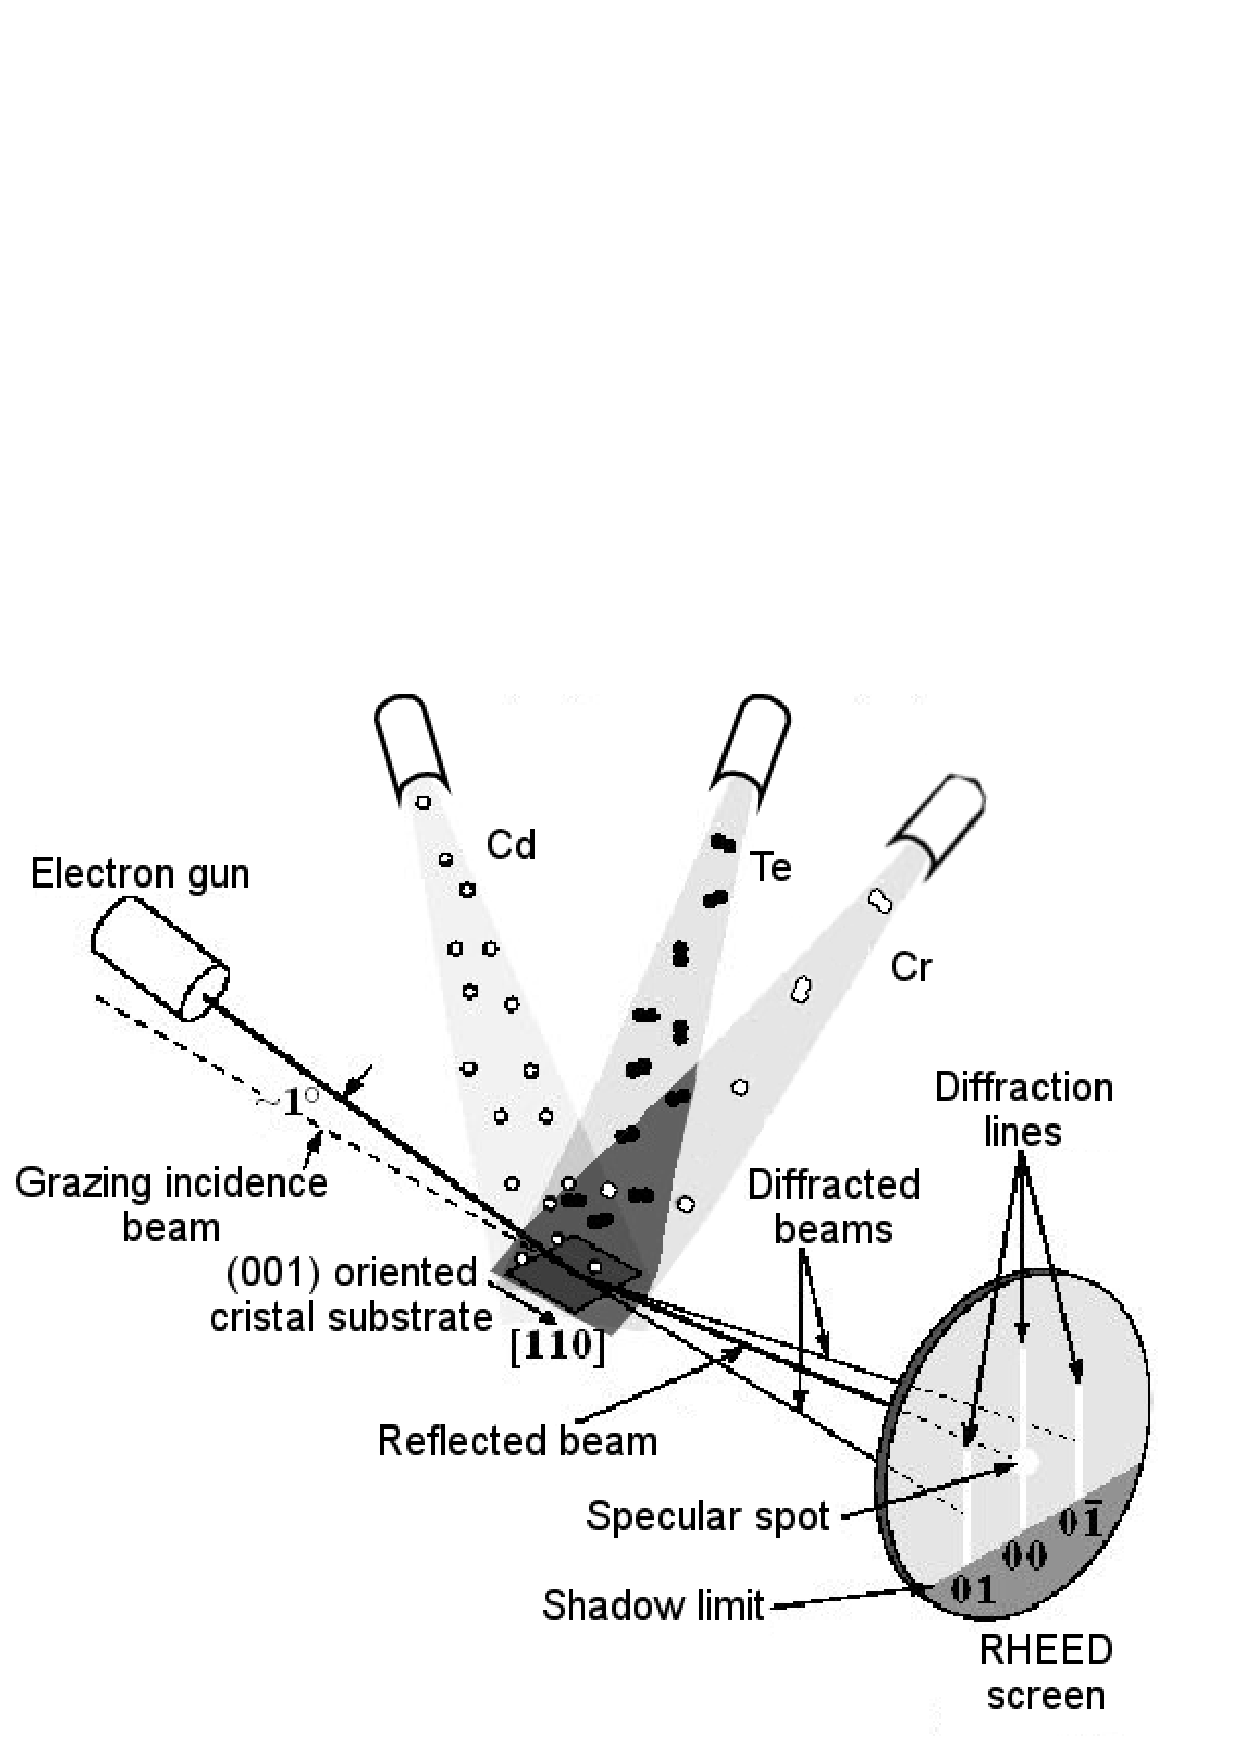
\includegraphics[width=10cm]{02-GrowthQDs/Pictures/MBE.png}
	\end{center}
	\caption{Schema of a MBE cells and substrate during a growth. An electron gun is attached to the chamber in order to probe the surface of the sample.}
	\label{MBEScheme}
	\end{figure}
	
	 The elements are kept in Knudsen cells, which consist of a crucibles of high-melting-point material wrapped in Tungsten filament acting as heater. A shutter is put in front of them to stop the element flux. During the growth, the shutter is opened to let the element travel to the substrate. The growth by MBE is a slow process: it can takes more than a hour to get a layer 1 $\mu$m thick. In order to avoid contamination, Ultra High Vacuum, in the order of $10^{-8}$ Pa, is needed. Under this condition, the mean free path of the gas is long compared to distance to the sample (km for the mean free path of gas, when the distance between the substrate and the cell is of the order of 50 cm). This process is illustrated in Fig.~\ref{MBEScheme}. Reaching the surface, the atoms diffuse before stopping, either having dissipated their kinetic energy through interaction with the surface, or (more commonly) being kept by islands steps created by previously deposited atoms. The growth occur layer by layer, slowly (about 1 ML/s), giving a good control of the thickness of the grown material.
		
	
	
	
	The growth can be monitored in-situ with RHEED (Reflexion High-Energy Electron Diffraction). An electron gun send a beam of high energy electrons, extracted from a filament by high bias voltage, at a low angle, between 1$^{\circ}$ and 3$^{\circ}$, to the surface sample. This way, the electrons will only probe the surface of the sample, penetrating the material only on a few MLs. From the difracted pattern, we can get information on the morphology of the surface. We can also use the variation of intensity of the specular spot, the spot at lowest angle reflected, to measure the growth rate of the deposited material, as illustrated on Fig.~\ref{RHEED}.
	
	\begin{figure}[h!]
	\begin{center}
		\includegraphics[width=12cm]{02-GrowthQDs/Pictures/EwaldRHEED.png}
	\end{center}
	\caption{(a) Construction of the Ewald sphere in the reciprocal space for an elastic scattering. For diffraction to occur, the reciprocal lattice must lie on the Ewald sphere. (b) Change of the RHEED pattern from a flat surface (left) to a rough one due to the formation of QDs (right). (c) Surface state during the growth of 2 MLs (left) and RHEED intensity for each step (right).}
	\label{RHEED}
	\end{figure}
	
	Incident electrons have a wave vector $\mathbf{k_i} = 2 \pi / \lambda_e$, with $\lambda_e$ the electron wavelength, typically 30 or 40 pm for an electrons at 30-40 keV. Since only scattered diffraction is considered, the diffracted wave vector $\mathbf{k_f}$ as the same module as the incident one $\mathbf{k_i}$. The Ewald's sphere has then a radius equal to $||\mathbf{k_i}||$. In the reciprocal space, the plane of diffraction are infinite line. So, in the case of a perfect crystal, with a perfect detector, the intersection with Ewald's sphere should be points. However, since the crystal may present some defects and neither the gun or the detector are perfect, the intersections appear as lines on the diffracted pattern.
	
	The growth of QDs makes the surface rough at the scale of the length of coherence of the beam. The electrons can interact with more layers while passing through the dots. This can be seen on the diffraction pattern, where lines become points.
	
	
	%We are working with two sample holder, named "marked" and "unmarked", with slightly different temperature offset. The thermometer to measure the substrate temperature is placed at a few centimetre from the substrate holder, inducing another offset in the measured temperature.
	
	\section{Self-assembled CdTe/ZnTe quantum dots doped with single Cr atoms\label{SK}}
	
	\subsection{Substrate preparation}
	
		The samples were grown on ZnTe(100) substrates. Two cleaning methods were tested:
		\begin{easylist}[enumerate]
			\ListProperties(Numbers=r, FinalMark={) })
			& etching of the substrate in a Bromide solution (Br$_2$-C$_2$H$_5$OH)
			& exposition of the substrate to a hydrogen radical plasma.
		\end{easylist}

		The etching process was done in four steps. All of them, except the etching in Bromide-ethanol, occured in an ultrasonic cleaning device vibrating the sample at 43 kHz for 3 minutes. We began with a cleaning in acetone, followed by one in ethanol. The third step was etching in Bromide-ethanol, with 3\% of Bromide, for 1 minute. We rinsed the sample in methanol. Once rinsed, we keep the sample in ethanol until mounting them on the sample holder. The transfer from the ethanol to the MBE chamber takes a few minutes, and some contamination might occurs during this time.
		
		In order to avoid contamination during the transfer, another type of cleaning of the surface was tried: using hydrogen radical (H$^*$) to remove the impurity at the surface. The substrate was rinsed four times, first in acetone, then ethanol and then water, for a duration of 5 min with sonication at 43 kHz, and finally 5 more minutes in water with sonication at 23 kHz. once the sample was clean, it was mounted on the sample holder and loaded in the MBE system. The hydrogen radicals  were formed in a seperate chamber by a RF power source operating at 13.6 MHz and at a power of 300 W. The substrate is exposed to the plasma for 15 min at 400$^{\circ}$C. The evolution of the surface was monitored with the RHEED: the diffraction pattern presented strikes after the exposition to H$^*$ plasma.
		
		Most of the sample we grew were done using the Br-ethanol etching. Cleaning by H$^*$ radicals was tested later during my PhD, and only a few containing Cr-doped dots. In this thesis, the only sample presented cleaned with the later technique is the charge control sample.
	
	\subsection{Stranski-Krastanov quantum dots growth\label{SKGrowth}}
	
	The self-assembled dots are formed using Stranski-Krastanov growth. A material with a different lattice parameter than the substrate is deposited. This lattice parameter difference create strain in the grown layer. Growing over the critical thickness, the layer may relax in different fashion, depending on the material. In Stranski-Krastanov growth, the relaxation occur via the formation of island, the QDs, on the layer. QDs formed by this method are called Stranski-Krastanov dots (SK dots). For CdTe/ZnTe, the critical thickness is $h_c = 6.5$ MLs~\cite{CritThickCdTeZnTe}. However, the dots does not form naturally in CdTe/ZnTe: if left as is, dislocation will form in the layer to relax the strains. In order to form the dots, a layer of amorphous Tellurite has to be deposited on the surface of the sample, and then evaporated~\cite{TinjodMBE}.
	
	The CdTe QDs layer is grown by Atome Layer Epitaxy (ALE), or Migration-Enhanced Epitaxy (MEE). While in classical use of MBE, the elements of the material are co-deposited on the substrate, in ALE, each cell is open one after the other, in sequence. Between each opening, the sample is left under vacuum in order to relax the surface. Such a growth is auto-regulated: when only one element is open, only a given quantity of material will be deposited and then the growth will stop until the other element is also deposited. The deposited quantity of material before the growth stop depends only on the substrate temperature. This allow for a really fine control of the growth and the deposited thickness is achieved. A full cycle correspond to opening each cell once.
	
	\begin{table}[h!]
	\begin{center}		
		\begin{tabular}{| c | c | M{4cm} |}
			\hline
			Elements & Targeted BEP (Pa) & Targeted flux (atoms.cm$^{-2}$.s$^{-1}$) \\ \hline
			Zn & $9.1\times10^{-5}$ & $1.3\times10^{14}$ \\
			Te & $6.0\times10^{-5}$ & $5.8\times10^{13}$ \\
			Cd & $6.0\times10^{-5}$ & $6.7\times10^{13}$ \\
			\hline
		\end{tabular}
		\caption{Targeted flux in Beam Equivalent Pressure (BEP) for each cell during the growth of the strained QDs.}
		\label{FluxTempSK}
	\end{center}
	\end{table}
	
	The targeted flux chosen for the growth of the CdTe/ZnTe QDs are presented in Tab.~\ref{FluxTempSK} for each cell used during the growth. These flux were measured via a Bayard-Alperd pressure gauge inside the MBE chamber, and are therefore given in Beam Equivalent Pressure (BEP). It was shown that the best quality of ZnTe was achieved for a growth in excess of Zn~\cite{TeEffect}. Otherwise, vacancies appear in the bulk, optically visible, and the surface is rougher. The ZnTe barriers were therefore grown in excess of Zn.
	
	The relative flux of the elements have no influence on the ALE process. We only have to be careful to deposit enough of each element to saturate the surface at each opening. We therefore chose to use the same flux for both Cd and Te~\cite{HMarALE}.
	

	\begin{figure}[h!]
	\begin{center}
		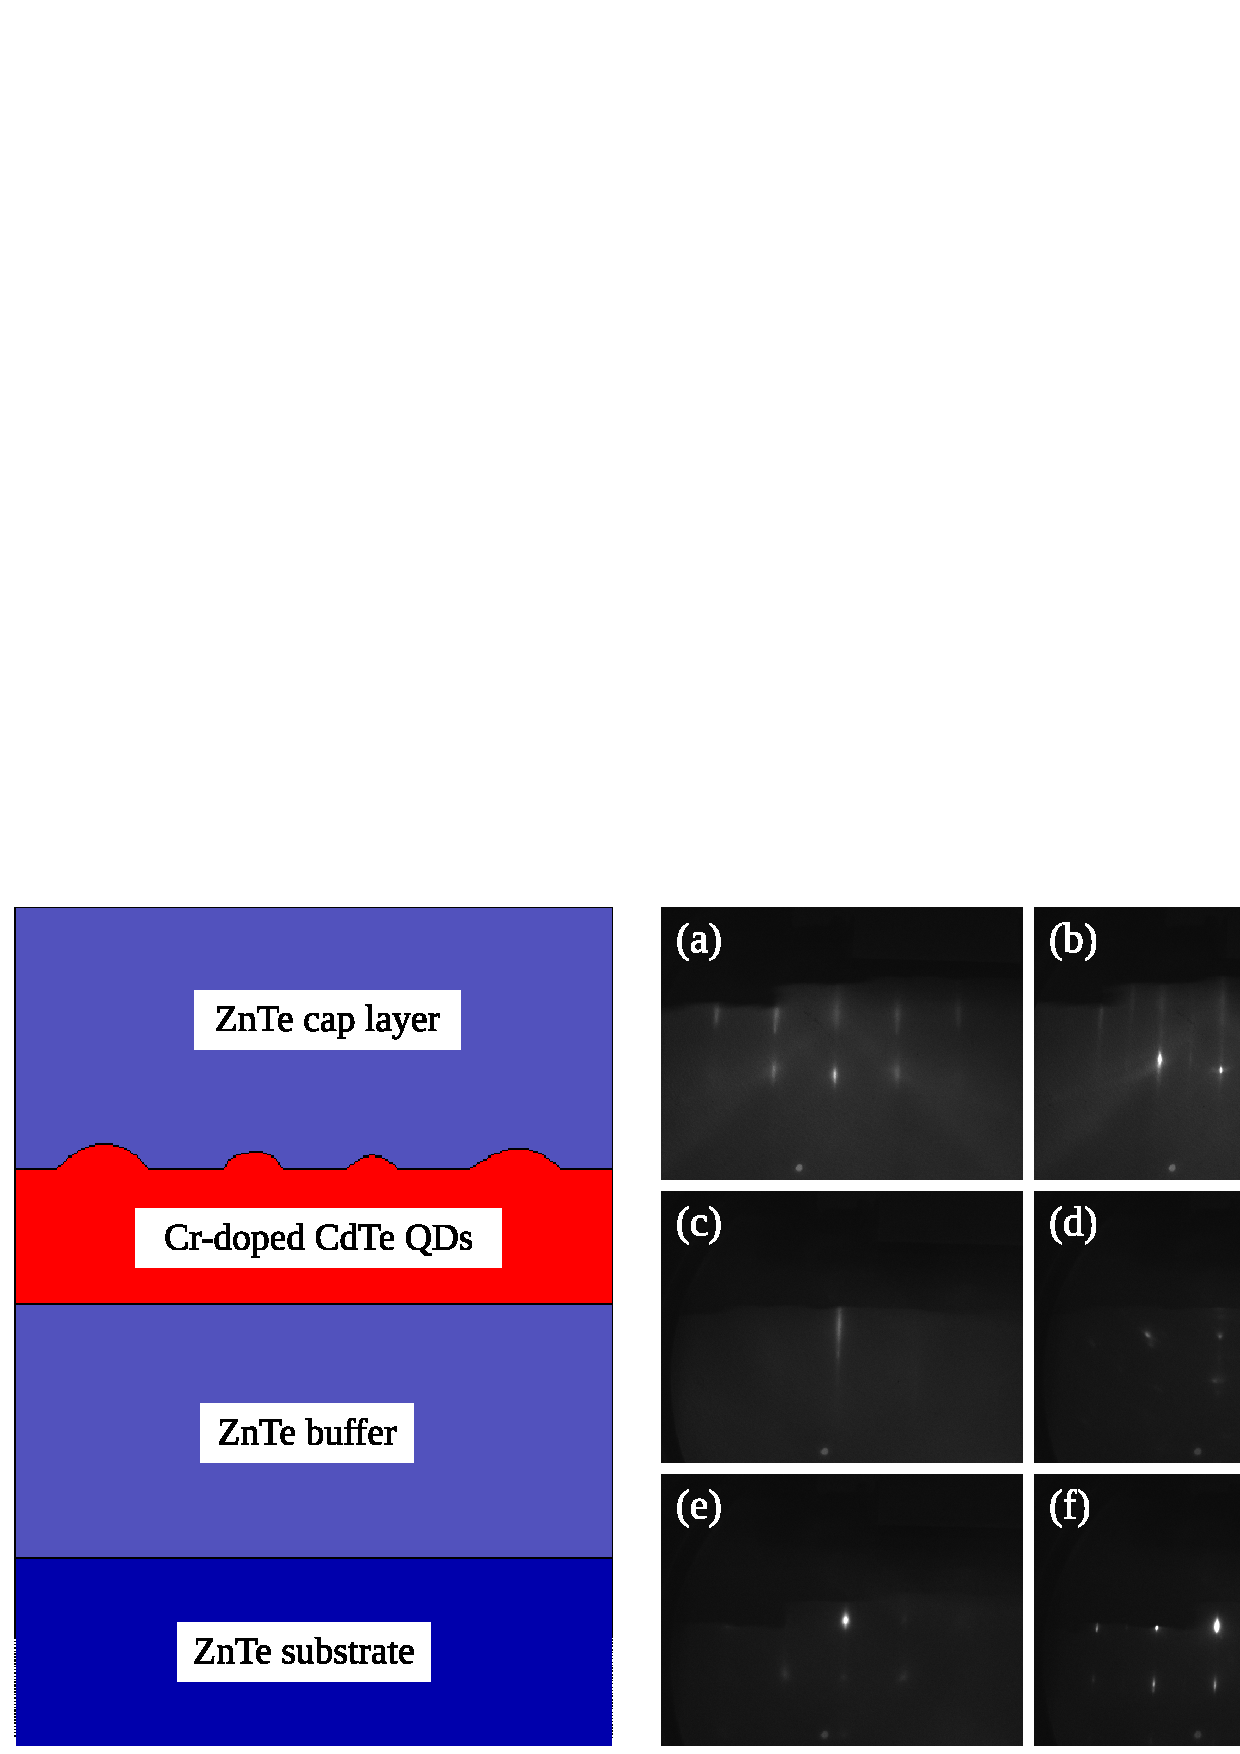
\includegraphics[width=14cm]{02-GrowthQDs/Pictures/RHEEDStep.png}
	\end{center}
	\caption{Left: Layer structure of the strain Cr-doped CdTe QDs samples. Right: RHEED pattern taken along the Te reconstruction line at different key moment of the growth: (a) before the growth of the ZnTe buffer, (b) after the growth of the ZnTe buffer, (c) end of the (Cd,Cr)Te layer deposition, (d) after the Te deposition, (e) after the Te evaporation (T$_{substrate} = 163^{\circ}$C) and (f) after the growth of the ZnTe cap.}
	\label{RHEEDStep}
	\end{figure}
	
	Beginning the growth, the substrate temperature was initially raised to $400^{\circ}$C. The Zn cell shutter was open starting at $355^{\circ}$C, in order to flatten the surface for the growth. While it took several minutes to raise the substrate temperature, the growth was stop by the auto-regulation of the ZnTe growth. When the substrate temperature reach $400^{\circ}$C, the Te shutter was also open, in order to grow the ZnTe buffer layer. This thick ZnTe layer keep us far from the substrate surface, that can have some default, and gives us a flat surface~\cite{ChangZnTe}. The surface quality is checked by RHEED, presenting clear diffraction lines (Fig.~\ref{RHEEDStep} (b)). The substrate temperature was then lowered to $295^{\circ}$C, the Zn cell being open until the temperature reach $355^{\circ}$C.
	
	CdTe is grown by ALE, in which the choice of substrate temperature fix the quantity of material deposited at each cycle. It was found that 0.5 ML of CdTe is deposited at each cycle for a substrate temperature between 260$^{\circ}$C and 290$^{\circ}$C~\cite{HMarALE}. Taking a temperature between those two limits allows for a small uncertainty on the substrate temperature while keeping a really good control on the growth of the sample.
	
	The growth during ALE was monitored via the intensity of the specular spot. Focusing on the lowest angle reflected spot, called the specular spot, one can see small variations in the reflected intensity during the growth. This is the same mechanism as the one presented in Fig.~\ref{RHEED} for the RHEED oscillation during the construction of the surface. Fig.~\ref{RHEEDOsc} presents oscillations taken during an ALE. Low intensity moments correspond to Cd deposition, high intensity to Te deposition. One can see series of low intensity, high intensity, medium intensity and high intensity repeating. Those corresponds to two ALE cycles, and therefore the growth of single CdTe monolayer~\cite{HMarALE}. We can also see the relaxation of a layer: the surface becomes then rougher, and the specular sport stays at low intensity.
	
	\begin{figure}[h!]
	\begin{center}
		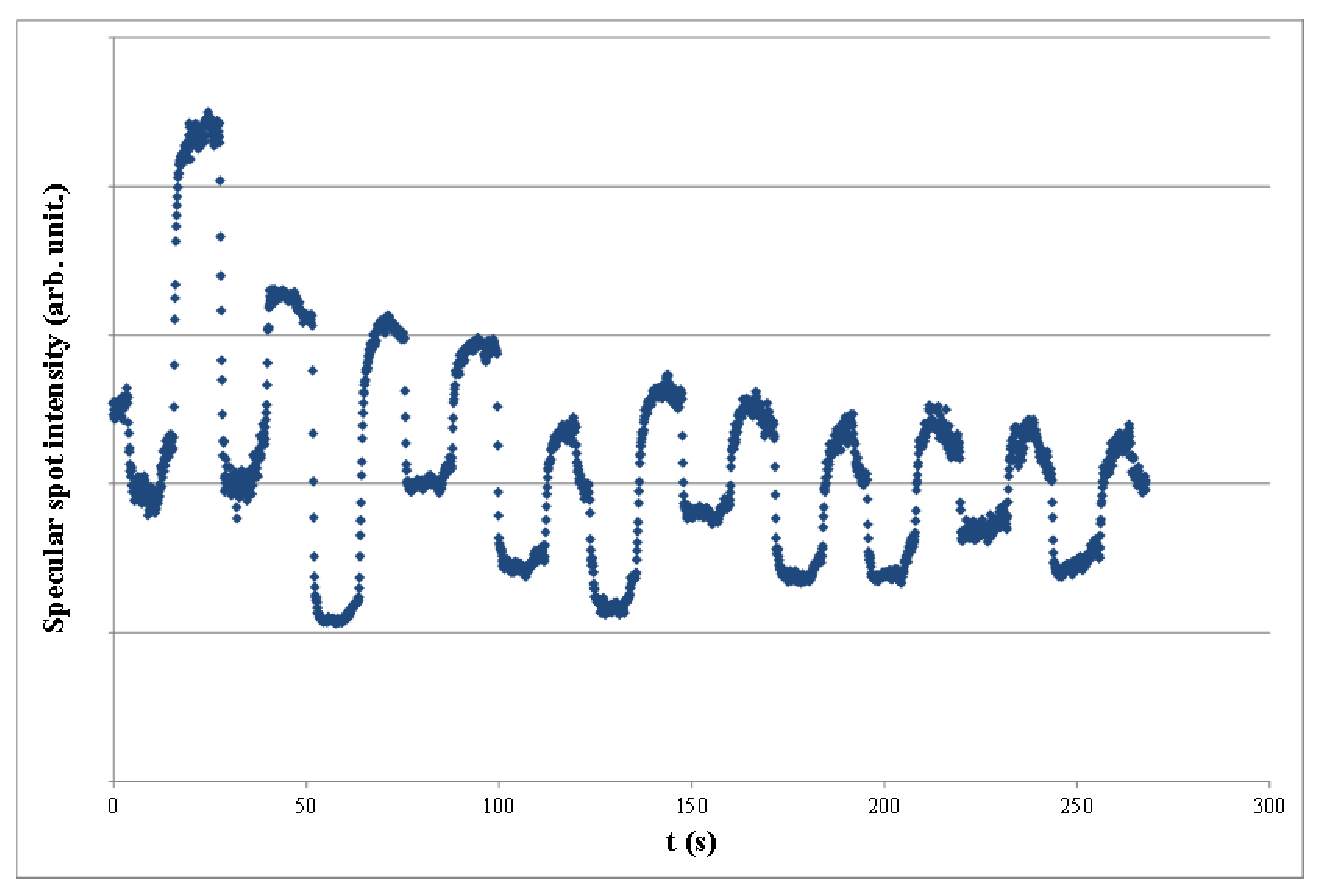
\includegraphics[width=12cm]{02-GrowthQDs/Pictures/RheedOsc.eps}
	\end{center}
	\caption{RHEED oscillation for the ALE of the strained dots.}
	\label{RHEEDOsc}
	\end{figure}
	
	One of the main goal of this work was to calibrate the Cr flux in order to optimize the probability of having a single Cr atom in most of the QDs of the sample. A first guess is that the Cr density must be of the same order as the QDs density at the surface of the sample. Supposing that all the Cr atoms get adsorbed on the sample, the quantity of deposited atoms is given by the flux of said atom times the time during which the cell stays open (exposition time). Due to the opening and closing time of the shutter, the exposition time cannot be shorter than a few seconds. Therefore a really small flux has to be chosen, with a BEP of the magnitude of $10^{-9}$ Pa, which is of the same order of magnitude than the main chamber pressure. It cannot therefore be not reliably measured using the gauge pressure. In order to find the cell temperature needed to reach such small flux, we used Arrhenius law, stating that the log of the flux of a cell varies linearly with the inverse of its temperature. From flux measured at higher temperature, we calculated the coefficients and deduced the aimed temperature of the Cr cell. The resulting curve is presented on Fig.~\ref{ArrLaw}, with coefficients values. The optimisation was done starting with the know how acquired in Grenoble on the growth of CdTe/ZnTe QD dopes with single Mn and trying to optimise it for the Tsukuba machine, through a feedback loop with the micro-PL characterization in Grenoble.
	
	\begin{figure}[h!]
	\begin{center}
		\includegraphics[width=12cm]{02-GrowthQDs/Pictures/ArrheniusCr.png}
	\end{center}
	\caption{Cr BEP as a function of 1000/T. Parameters of the Arrhenius law are given in the top left.}
	\label{ArrLaw}
	\end{figure}

	This really small flux was achieved by heating the Cr cell around 1000$^{\circ}$C, and opening the cell only once during the deposition of the CdTe layer. In order to have QD emitting in the right range of wavelength for our optical setup (around $\lambda = 600$ nm), the optical CdTe thickness is 6.5 MLs. However, this is close to the critical thickness. Therefore, to diminish the risk of dislocation in the CdTe layer, some samples were grown with 5.5 MLs of CdTe. The Cr cells was opened when half of the CdTe layer was grown (7th cycle for the 6.5 MLs samples, 5th cycle for the 5.5 MLs samples). The ALE sequences used to grow the CdTe layer is shown in Fig.~\ref{RecipeSK}.
	
	\begin{figure}[h!]
	\begin{center}
		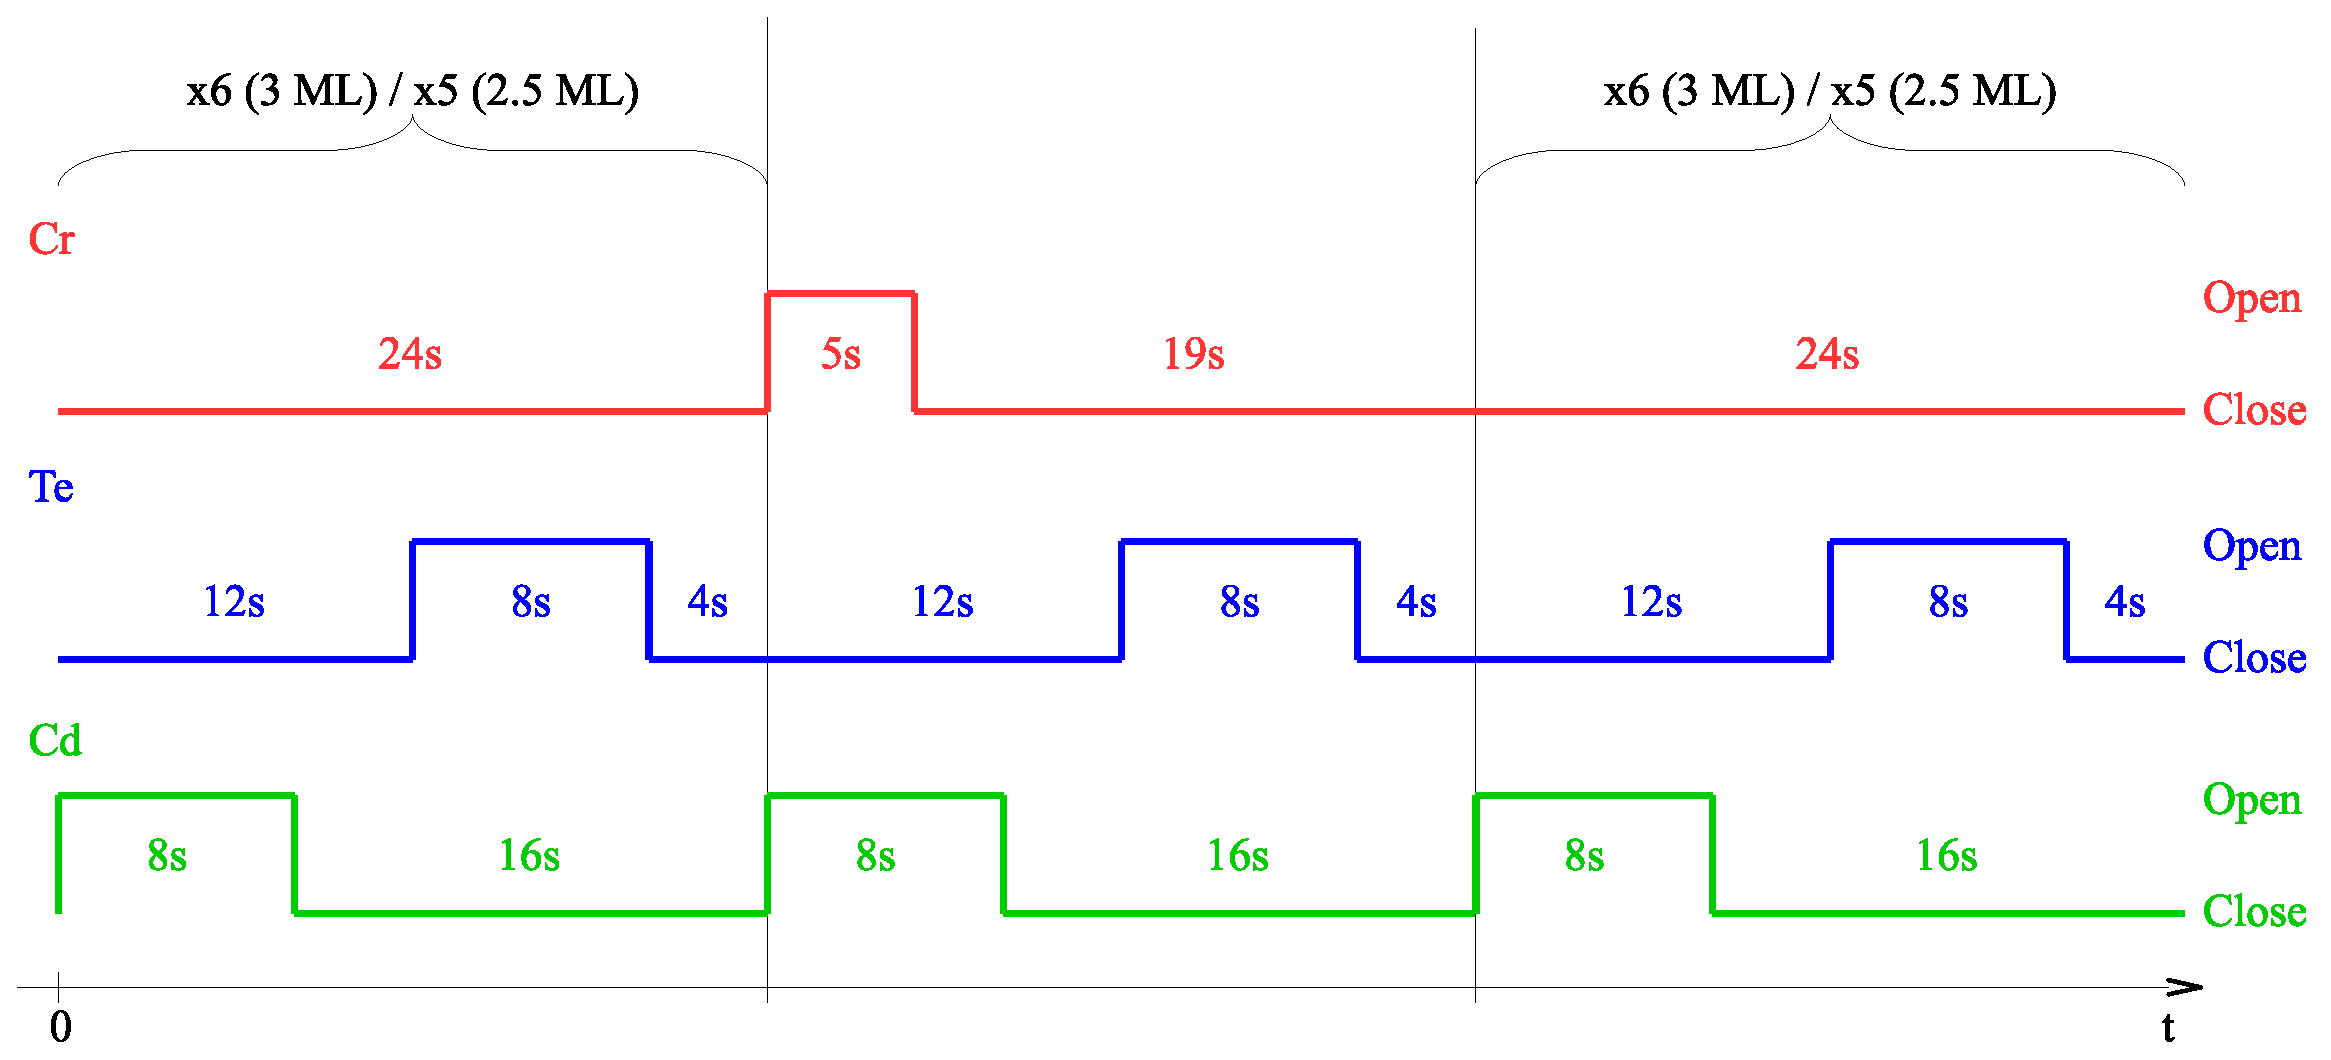
\includegraphics[width=13cm]{02-GrowthQDs/Pictures/RecipeSK.eps}
	\end{center}
	\caption{Opening and closing cycles of each cells used to grow either 6.5 MLs or 5.5 MLs of (Cd,Cr)Te for the formation of Cr-doped SK dots.}
	\label{RecipeSK}
	\end{figure}

	After the growth of the CdTe layer, we lowered the substrate temperature to $210^{\circ}$C to deposit an amorphous Te layer. It was deposited during 5 minutes. We then heated up the substrate again to $320^{\circ}$C, were we stayed for 20s in order to evaporate all the deposited Te~\cite{WojnarMBE}. The formation of dots was confirmed by a spotty diffraction pattern like the one presented on Fig.~\ref{RHEEDStep} (f). The Zn and Te cells were then opened, while the substrate temperature was raised to $350^{\circ}$C in order to grow a protective layer of about 50 nm of ZnTe above the QDs.
	
	\subsection{Optical characterization}
	
	The samples were studied in Grenoble, at the Neel Institute. The characterization of the samples was done in two steps. First, we took macro-photoluminescence spectra, on a large energy range, typically between 1.8 and 2.3 eV, with a laser set at 2.9 eV. This allow us to test the PL of the sample. As said in Sec.~\ref{CrSemiCon}, if the Cr concentration is too high, it may kill the PL of the dot layer, and thus it will not be seen in the macro-PL. If luminescence from the sample is seen in macro-PL, the sample is studied by micro-photoluminescence ($\mu$-PL), on a much narrower energy band (about 10 meV), to study dots individually. A high refractive ($n \approx 2.5$) index hemi-spherical Solid Immersion Lens (SIL) was mounted on the sample before their study, to improve the spatial resolution and enhance the collection efficiency of a single dot photoluminescence (PL) in a low temperature optical microscope. The sample is scanned randomly. We judge the quality of the sample by the number of actual dots we found with single Cr embedded inside, and by the proportion of thin emission peaks (a few tens of $\mu$eV) versus broad ones (in the meV range): if we saw mainly broad peaks, it suggests that the Cr concentration is too high.
	
	\begin{table}[h!]
		\begin{center}
			\caption{List of samples where single dots with single Cr was found.\label{SKsamples}}
			\begin{tabular}{M{2cm}|M{3cm}|M{2cm}|M{3.3cm}|M{2.2cm}}
				Sample name & Cleaning process & \# CdTe MLs & Targeted Cr concentration (\%) & \# Cr-doped dots found\\
				\hline
				dot334 & Br etching & 6.5 & 0.09 & 3 \\
				dot338 & Br etching & 6.5 & 0.05 & 2 \\				
				dot359 & Br etching & 6.5 & 0.11 & 1 \\
				dot363 & Br etching & 6.5 & 0.21 & 2
			\end{tabular}
		\end{center}
	\end{table}
	
	The samples where QDs doped with a single Cr atom were found are listed in Tab.~\ref{SKsamples}. The Cr concentration in the sample was estimated using the Cr flux. The Cr composition is given as percentage of the cation site occupancy (Cd$_{1-x}$Cr$_x$Te). We see that correct samples were found for a large range of concentration. The probability to find good Cr-doped dots in dot338 and dot363 is about the same. However, dot363, with the higher Cr targeted concentration, presents a lot of broad peaks. All samples grown with a Cr concentration higher than 0.20\% had a luminescence too weak to be studied properly. We can estimate that the good range of concentration is between 0.05\% and 0.20\%. Some more test have to be done in order to fine tune the Cr composition.
	
	\section{Charge tunable samples and strain-free samples}
		\subsection{Charge tunable samples\label{ChargedSample}}	
		
	The charge control samples are grown in order to be able to apply an electric field on the dot layer. The growth occurs on a p-doped ZnTe substrate. It gives the sample a conductive back. The growth was done in order to form Stranski-Krastanov dots, as described in the previous section. All the charge tunable samples were clean using H$^*$ plasma. Thinner buffer and cap layers were necessary in order to be able to apply a stronger electric field on the dot layer. We chose thicknesses between 150 nm and 200 nm for the buffer, and of 110 nm for the cap.
	
	\begin{figure}[h!]
	\fcapside{\caption{Schema of the charge control structure, on a p-doped ZnTe substrate and with a thin, semi-transparent gold layer deposited on the surface.}\label{ChargeContSample}}	
	{\begin{center}
		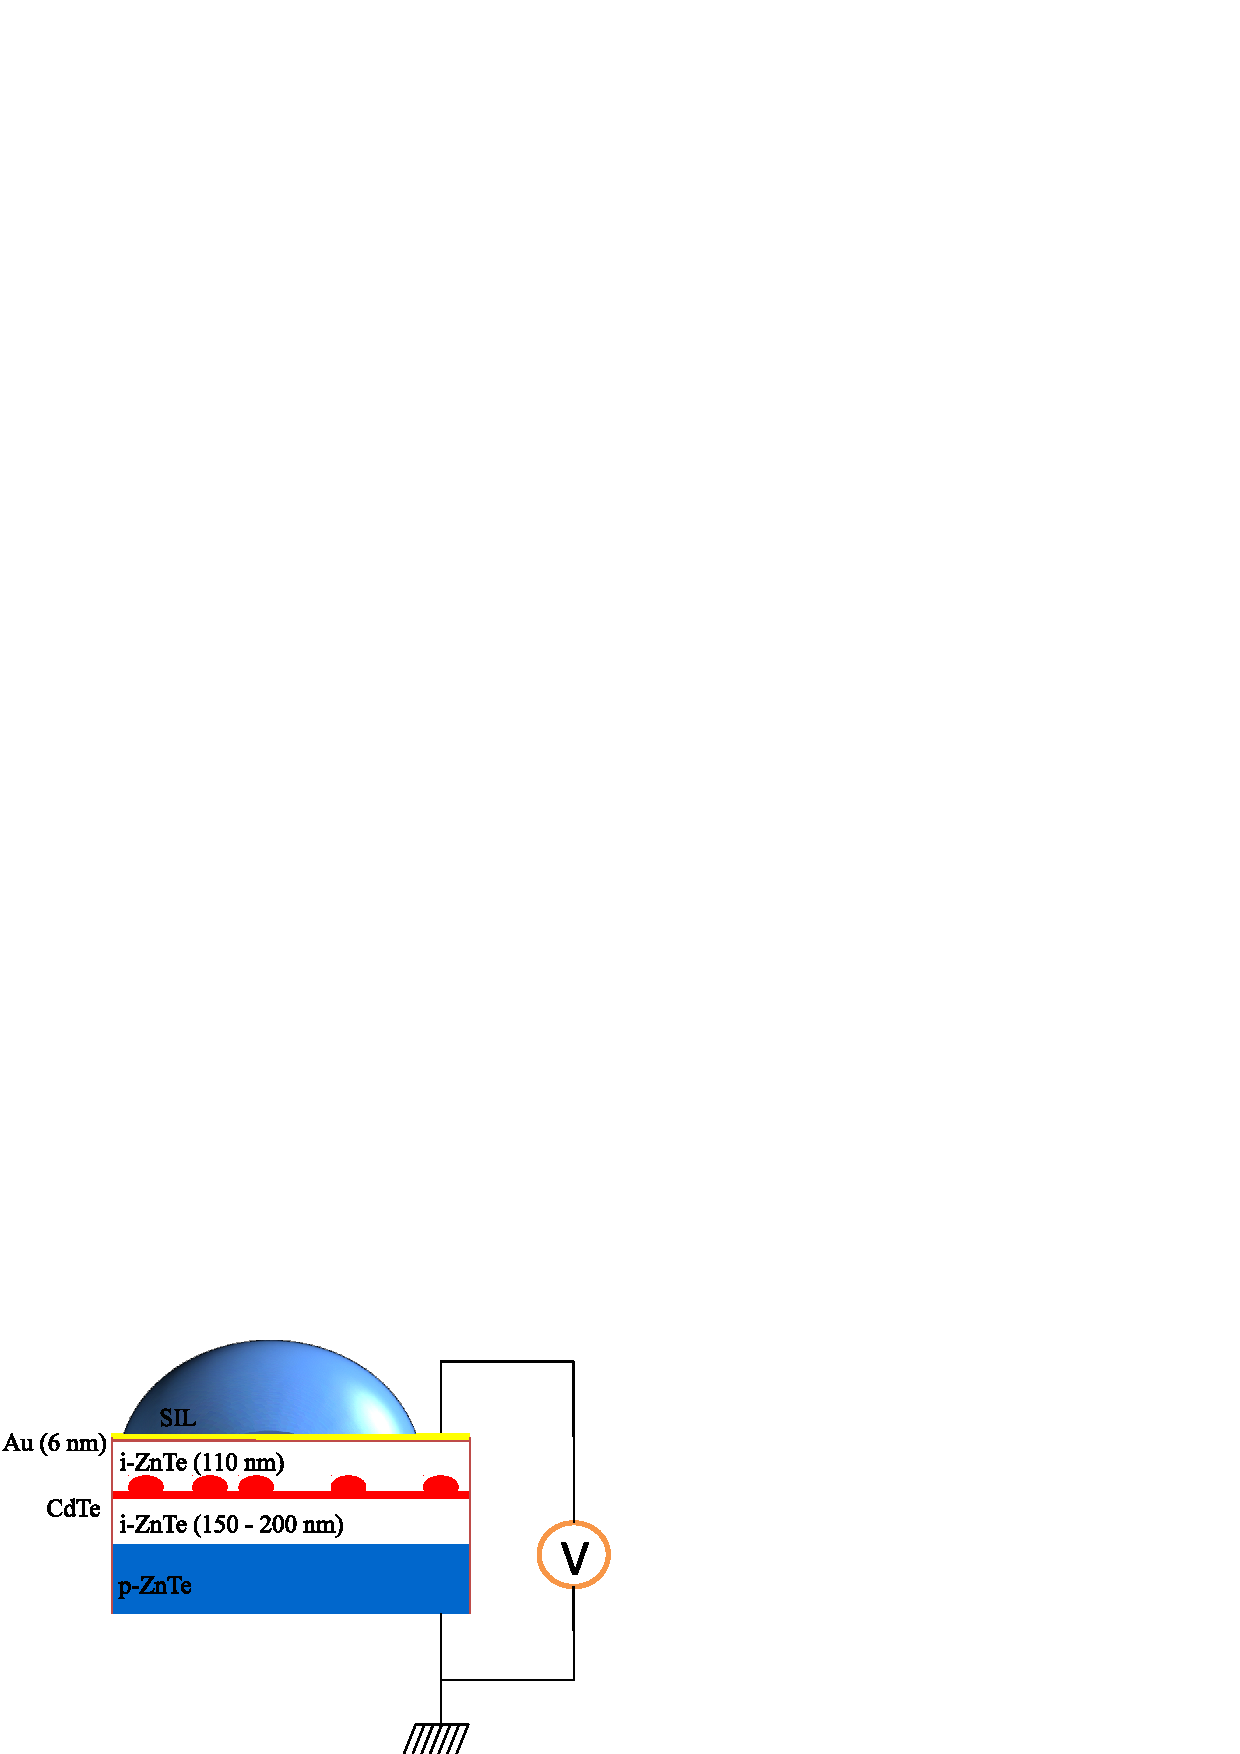
\includegraphics[width=7.4cm]{02-GrowthQDs/Pictures/ChargeContSample.png}
	\end{center}}
	\end{figure}
	
	The conductive surface was formed by a thin, semi-transparent gold layer, forming a Schottky junction with the sample cap layer. It was deposited by sputtering just after the MBE growth in order to keep a clean surface. The samples were kept in nitrogen atmosphere during the transport between the MBE and the sputtering machine. A deposition time of 35 s was chosen. Fig.~\ref{ChargeContSample} shows a schema of the sample as it was studied.
	
	Only one Cr-doped charge tunable sample was grown and studied during this PhD, named dot390. It was decided to make the CdTe layer 5.5 MLs thick in order to not have dislocation in the QD layer. The targeted Cr concentration was 0.16\%.
	
 	\subsubsection*{Optical characterization}
	
	In order to test the application of bias voltage in the sample, we glued two electrodes with silver lacquer. A SIL was mounted on top of the sample. We looked at the PL of single dots and see their evolution under the application of a bias voltage. Fig.~\ref{ChargeVar} (a) presents the results of such an experiment.

	\begin{figure}[h!]
	\begin{center}
		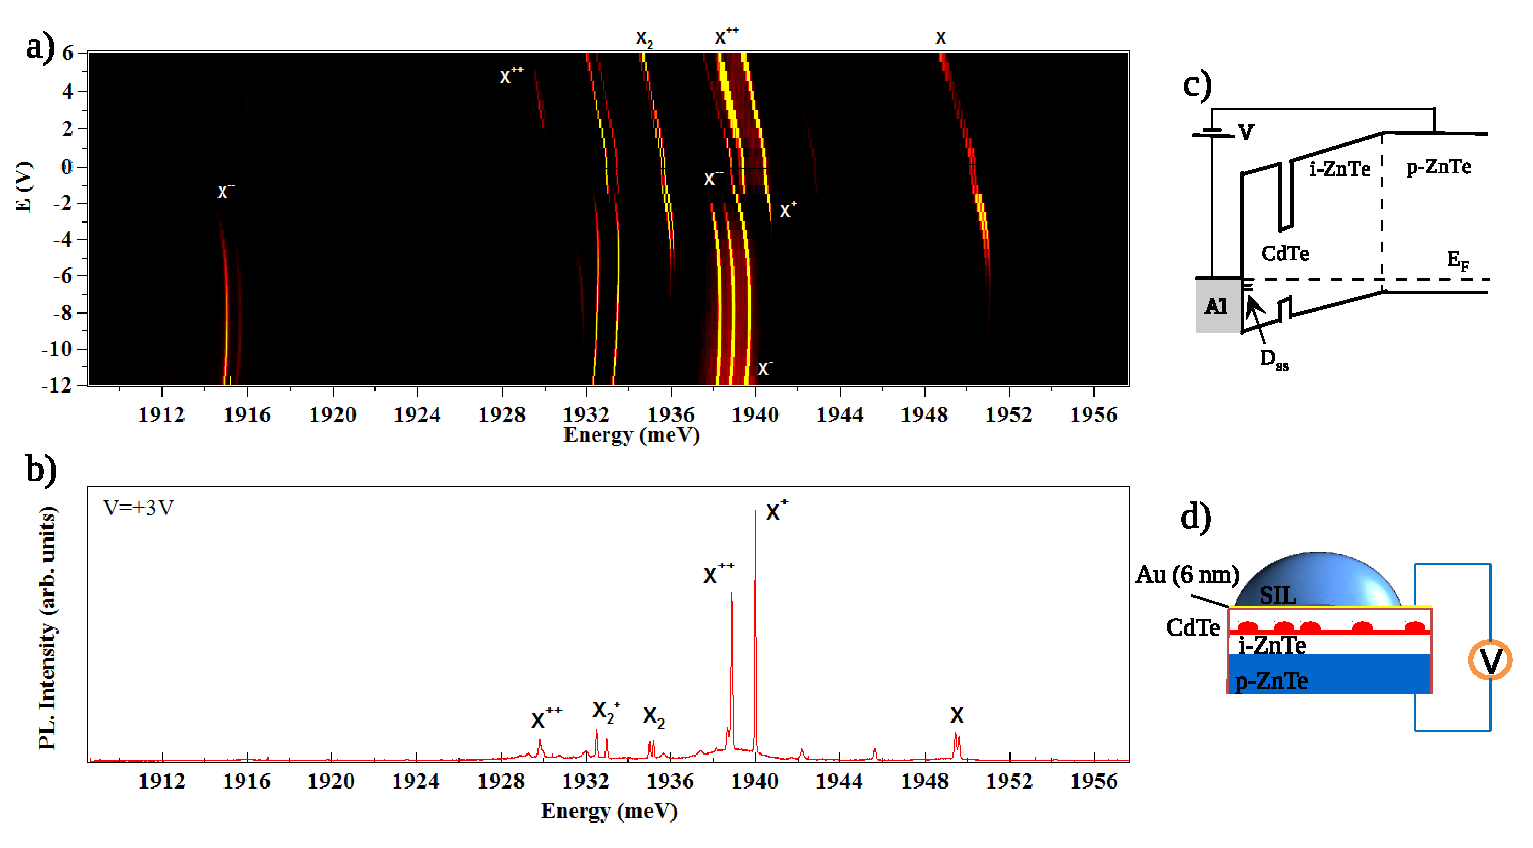
\includegraphics[width=10.5cm]{02-GrowthQDs/Pictures/MapEfield.eps}
	\end{center}
	\caption{(a) Evolution of the PL of a single dot under application of a bias voltage V. Below are presented spectra of the dot taken under three different values of bias voltages: (b) V = $+3$ V (positively charged), (c) V = $-1.5$ V (neutral) and (d) V = $-8$ V (negatively charged). Identification of the different species was done following ref.~\cite{BesombesIdentificXSpecies}.}
	\label{ChargeVar}
	\end{figure}

	The main result of the experiment is the appearance of different excitonic species depending on the applied electric field. The spectrum are dominated by the neutral state of the quantum dot for an applied electric field of V = -1.5 V (Fig.~\ref{ChargeVar} (c)). At this voltage, the neutral excitonic species X and X$^2$ are the strongest. Charged excitons still appear because of charge variations occuring close to the QD, injecting electron or holes inside it. Further lowering the bias voltage, the probability of the dot to be negatively charged increases. Neutral excitonic species disappear and the peaks of the negatively charged species (X$^-$, X$^{--}$ and X$_2^-$) become dominant. A spectra taken at V = -8 V is presented on Fig.~\ref{ChargeVar} (d). One can notice that, X$^{--}$ is splitted into two group of two peaks, around 1917.5 meV and 1933 meV on Fig.~\ref{ChargeVar} (d). It is caused by the electron-electron interaction and has already been observed in InAs quantum dots~\cite{FineStructX2charge}. On the contrary, applying a positive bias voltage increases the probability to detect positively charged exciton complexes, maximizing X$^+$ and X$^{++}$ intensity. This is shown on Fig.~\ref{ChargeVar} (b) for a bias voltage of V = +3 V. This shows that we can select efficiently the charge of a quantum dot applying a bias voltage across it.
	
	
	dot390 was studied under $\mu$-PL. However, no Cr doped quantum dots were found. Some dots looking like dots doped with a single Cr atom were found, but further investigation shows no sign of magnetic atom in them. Such QDs are discussed in more details in Sec.~\ref{ChargeFluc}.
	
		\subsection{Strain-free quantum dots\label{SFD}}
		

	
	In SK dots, the some strain remain in the QD layer, and we have no control on them. As will be discussed later, remaining strains limits the life-time of the Cr spin. We decided therefore to grow strain-free dot to get rid of those limits. They are formed by the thickness fluctuations of a CdTe quantum well in Cd$_{0.7}$Mg$_{0.3}$Te barriers, grown on a CdTe substrate. These fluctuations form steps localizing the carriers, acting as QDs. We chose to use Cd$_{0.7}$Mg$_{0.3}$Te to keep a lattice parameter close enough to CdTe to grow thick enough barriers, and keeping enough gap difference to localize the carriers. The needed flux for this growth are shown in Tab.~\ref{FluxTempSFD}.
	
	\begin{table}[h!]
	\begin{center}		
		\begin{tabular}{| c | c | M{4cm} |}
			\hline
			Elements & Targeted BEP (Pa) & Targeted flux (atoms.cm$^{-2}$.s$^{-1}$) \\ \hline
			Cd & $6.0\times10^{-5}$ & $6.7\times10^{13}$ \\
			Mg & $2.1\times10^{-6}$ & $4.7\times10^{12}$ \\
			Te & $7.0\times10^{-7}$ & $5.8\times10^{13}$ \\
			\hline
		\end{tabular}
		\caption{Aimed flux for each cell during the growth of the strained samples.}
		\label{FluxTempSFD}
	\end{center}
	\end{table}
	
	The critical thickness of Cd$_{0.7}$Mg$_{0.3}$Te on CdTe is not exactly known. Systematic studies were done on CdTe/CdZnTe gives an empirical law to calculate the critical thickness~\cite{CritThickCdTeCdZnTe}. This law was used for different II-VI material and gives a good approximation of the different critical thickness, overestimating slightly the effects of strain. For CdTe/Cd$_{0.7}$Mg$_{0.3}$Te, we found a critical thickness $h_c = 130$ nm. We chose to grow 40 nm below the QW, and 90 nm above it, to keep the surface far from the quantum well.
	
	The strain-free sample were grown on a hybrid substrate formed by a thick CdTe layer grown on GaAs. It was done on a fourth of a 2 inches GaAs substrate and protected by Te. The GaAs substrate was cleaned using H$^*$ plasma. A thin layer (about 7 nm) of ZnTe was first grown at 415$^{\circ}$C in order to get the right crystal orientation when growing the CdTe layer. We then grew a CdTe layer of about 3 $\mu$m at 360$^{\circ}$C, to recover a good crystallinity of the CdTe layer~\cite{StrainRelaxCdTeGaAs111}. The RHEED taken after the growth of the CdTe layer (Fig.~\ref{Hybrid} (d)) shows sharp straight line, showing the recovery of a flat surface.

	\begin{figure}[h!]
	\begin{center}
		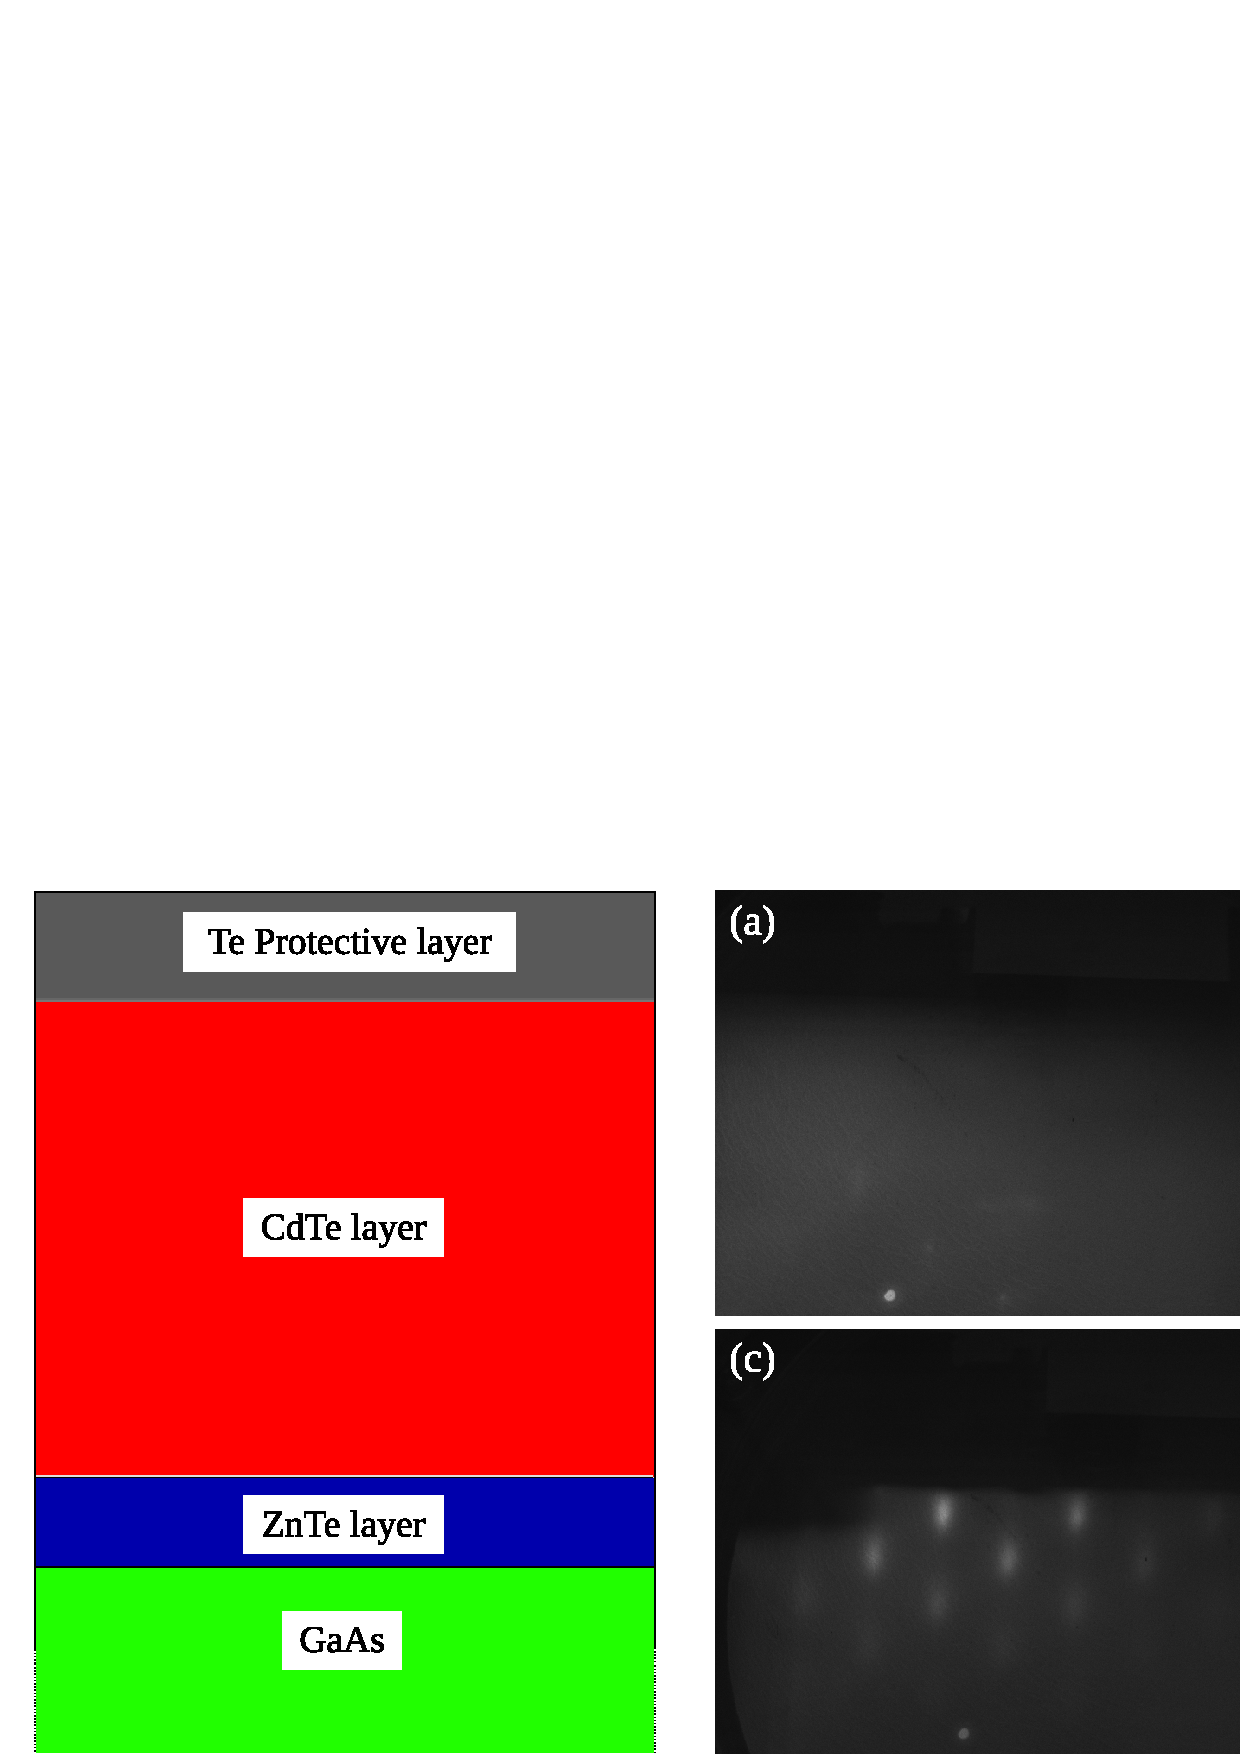
\includegraphics[width=14cm]{02-GrowthQDs/Pictures/HybridSubstrate.png}
	\end{center}
	\caption{Left: Layer structure of the hybrid substrate with its protective Te cap.
		Right: RHEED pattern taken at different key moment of the growth: (a) before H$^*$ cleaning of GaAs, (b) after H$^*$ cleaning of GaAs, (c) after the growth of the ZnTe layer, (d) after the growth of the CdTe layer.}
	\label{Hybrid}
	\end{figure}
		
		
	
	For the growth of strain free samples, we began to heat the substrate temperature to 300$^{\circ}$C and waited a few seconds to remove all the deposited Te; We then heated the sample to $360^{\circ}$C. Starting at $320^{\circ}$C, we opened the Te cells in order to stabilize the surface. When the substrate temperature was stabilized at $360^{\circ}$C, we opened the Cd cells and grew a 2.35 $\mu$m of CdTe on top of the 3 $\mu$m grown on the hybrid substrate, in order to be get far from the surface that might have been slightly damage during the conservation or the Te evaporation.
	
	\begin{figure}[h!]
	\begin{center}
		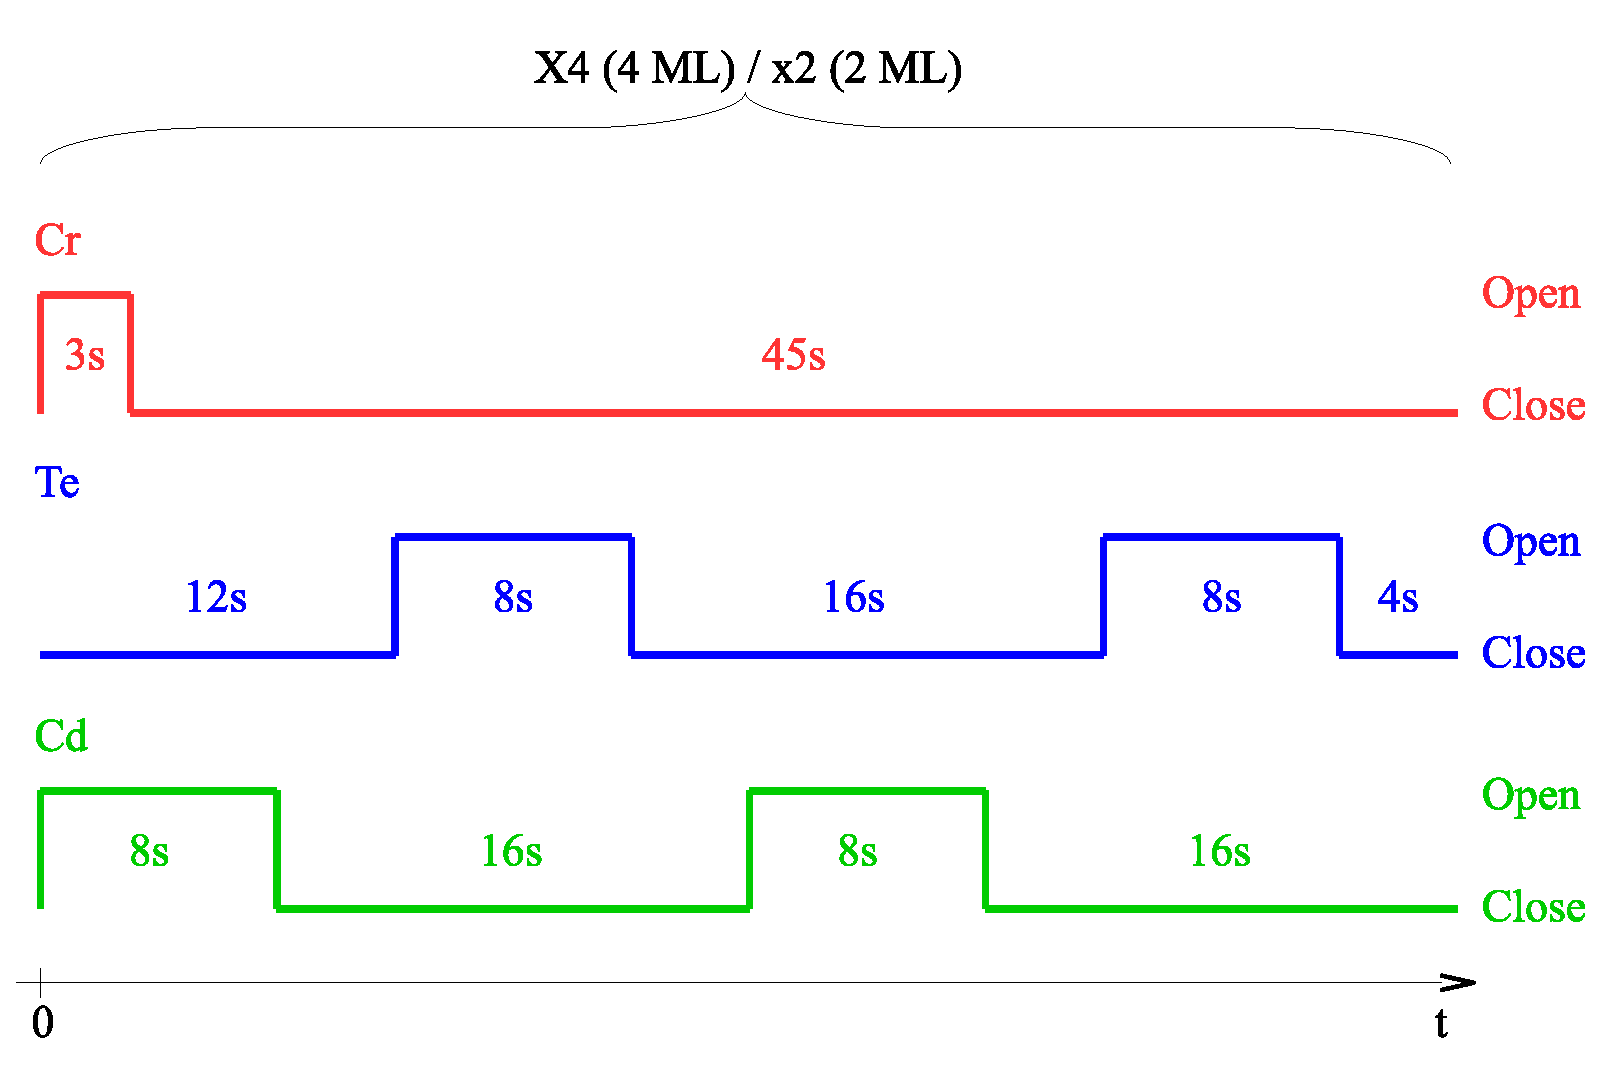
\includegraphics[width=10cm]{02-GrowthQDs/Pictures/RecipeSFD.eps}
	\end{center}
	\caption{Opening and closing cycles of each cell for the ALE of strain free (Cd,Cr)Te samples.}
	\label{RecipeSFD}
	\end{figure}
	
	We grew the 40 nm Cd$_{0.7}$Mg$_{0.3}$Te barrier on this buffer layer. Once the done, we lowered the substrate temperature under Te flux, in order to smoothen the sample surface. Once the substrate temperature reach $295^{\circ}$C, we began the ALE of the QW. Two QW thicknesses were tested: 4 ML and 2 ML. The Cd and Te cycles were the same as for the SK dots. The Cr, however, was open for only 3 s, but once every two cycles, for a total of 4 opening in the 4 ML case, and 2 opening for the 2 ML case. The whole recipe is described in Fig.~\ref{RecipeSFD}.
	
	We then raised the substrate temperature up to $360^{\circ}$C, under a Te flux, in order to proceed to the growth of the upper barrier, acting also as a protective layer. The opening time was there calculated to grow 90 nm of Cd$_{0.7}$Mg$_{0.3}$Te.

	\subsubsection*{Optical characterization}
	
	Four samples of strain-free dots doped with Cr were produced (see Tab.~\ref{SFDsamples}). The Cr concentration were taken high because it was see on the strain-free dots grown in Grenoble that a higher concentration of Mn was needed in strain-free dots than in SK dots. It was supposed to be the same with Cr. The Cr concentration was later rose after no dot doped with a single Cr was found.
	
	\begin{table}[h!]
		\begin{center}
			\caption{Strain-free QDs doped with Cr.\label{SFDsamples}}
			\begin{tabular}{M{2cm}|M{2.5cm}|M{3.5cm}|M{3cm}}
				Sample & \# CdTe MLs & Cr aimed concentration (\%) & Probability of Cr-doped QD \\
				\hline
				SFD4 & 4 & 0.35 & None found \\
				SFD5 & 2 & 0.15 & None found \\
				SFD6 & 2 & 0.54 & None found \\
				SFD7 & 2 & 0.35 & None found \\
				SFD8 & 2 & 0.75 & None found
			\end{tabular}
		\end{center}
	\end{table}
	
	
	The sample presented thin and intense peaks, as shown in Fig.~\ref{SpectraSFD}. It hints at a better confinement of the carriers in the QDs than the strain-free dots grown in Grenoble. This may be caused by higher steps than expected at the CdTe/Cd$_{0.7}$Mg$_{0.3}$Te interface.
	
	\begin{figure}[h!]
	\begin{center}
		\includegraphics[width=10cm]{02-GrowthQDs/Pictures/SFDSpectra.eps}
	\end{center}
	\caption{(a) Macro-PL of a SFD5. (b) Examples of spectra taken under $\mu$-PL in SFD5.}
	\label{SpectraSFD}
	\end{figure}
	
	As discussed in Sec.~\ref{XMn}, the presence of a magnetic atom splits the emission of the exciton into several peaks, the number depending on the spin of the magnetic atom. Such complex was not found in the strain-free samples. This may be caused by a problem in the Cr incorporation. The Cr possibly is not well embedded in the QW layer. More tests have to be done, depositing the Cr at different moment of the growth.
	
	Another possible cause of this absence could lie in the absence of strain. In SK dots, the presence of strains increases the probability of the Jahn-Teller deformation to occur along the $z$ axis. In strain-free dots, all direction are equivalent, and we expect two third of the Cr-doped dots to be undetectable because they are quantized in the plane, creating no splitting visible in our setup.
	
	In order to increase the probability for the Cr to be quantized along the $z$ axis, it is proposed to slightly strain the quantum well. This might be done by growing the sample on Cd$_{0.96}$Zn$_{0.04}$Te instead of CdTe. The lattice parameter of Cdte and Cd$_{0.96}$Zn$_{0.04}$Te have a lattice mismatch of only 0.3\%, so the strain it will create in the lattice should remain weak. They should however be enough to increase the probability of a deformation along the $z$ axis, making more dots visible in our setup.
	
	\section*{Conclusion}
	
	We saw in this chapter how we grew the samples studied in the next chapters. The samples were characterized in Grenoble. SK dots with single Cr atom embedded were found and studied. New Cr concentration were tested in Tsukuba after the feedbacks from Grenoble. More tests have to be done to increase the probability of finding dots doped with a single Cr atom.
	
	First step toward new kind of sample were also done: strain-free QD with single Cr, and SK dots with single Cr embedded in a field effect structure. Localized carrier emission was detected in the former, and we successfully applied bias voltage on the later. However, for both, no Cr-doped dots were found in. More tests have to be done to optimize their growth.








\chapter{Spin dynamics in Mn-doped positively charged quantum dots\label{CoDynMn}}

	%Bi-exciton was studied by Lucien Besombes \emph{et al.} a few years ago~\cite{}.

	Magnetic anisotropy depends on the local environment of magnetic atoms, and are a crucial properties for modern storage devices. We saw in Sec.~\ref{MnSemiCon} that the Mn atom in neutral, self-assembled QD presents a small anisotropy of a few tens of $\mu$eV. It is expected that a Mn atom could develop a large anisotropy energy in the meV range when it is exchange coupled with a single confined heavy-hole spin~\cite{VybornMagAnisoDopedQD}. The two low energy hole-Mn state behave like an Ising spin system, forming an atomic ferromagnet. In addition the exchange induced Mn spin magnetic anisotropy could be electrically controlled by changing the Mn/hh overlap with a bias voltage applied across the QD.
		
	In this chapter, we look at the spin dynamics of a Mn spin coupled to a single hole in a CdTe/ZnTe QD. We begin presenting the energy structure of this system. We show that $\Lambda$-level systems are formed between the hybrid spin states formed by the hole-Mn system in the ground state, and the electron-Mn states in the excited state. Those systems can be addressed independently with a resonant laser and are used to study the dynamics of the hole-Mn hybrid spin.
	
	In the second section, we study the dynamics of the h-Mn hybrid spin through two experiments: auto-correlation of the resonant PL and resonant optical pumping experiments. We identified an efficient relaxation channel for this hybrid spin via the interplay of the exchange interaction between the hole and the magnetic atom, as well as the coupling to accoustic phonons. We also show that the optical $\Lambda$-systems are connected through inefficient spin-flips that can be enhanced under weak transverse magnetic field. The dynamics of the resonant PL of a p-doped magnetic QD is well described by a complete rate equation model.   	
	
	In the last section, we look at the electron-Mn coherent dynamics, directly observed in the time resonant PL. Quantum beats reflecting the coherent transfer of population between e-Mn spin states, mixed by an anisotropic strain in the plane of the quantum dot, are clearly observed. We highlight that this strain induced coherent coupling is tunable with an external magnetic field.

	\section{Mn in a positively charged CdTe quantum dot}

		
		\subsection{Spin structure of a positively charged Mn doped quantum dot\label{hMnSpinStruct}}
		
		We saw in Sec.~\ref{XMn} that the exchange interaction between the hole and the Mn spin lifts the degeneracy of the Mn spin states. The recombination of the exciton states are then  each split into six lines. For a given polarization, each line corresponds to a given Mn spin state. The ground state of a Mn-doped positively charged quantum dot is formed by a single hole coupled to the Mn atom, leading to the same kind of splitting. Via the application of a positive bias voltage (V > 0) on the sample with a Schottky gate (see Sec.~\ref{ChargedSample}), a single hole is trapped in the magnetic QD and the emission of the positively charged exciton becomes largely dominant (Fig.~\ref{hMnspectra} (a)). The PL of such a QD is presented in Fig.~\ref{hMnspectra} (b).
		
	\begin{figure}[h!]
	\fcapside{\caption{(a) Color scale plot of the PL intensity of one QD of sample M3085, embedding a single Mn inserted in Schottky structure, showing the emission of the neutral (X-Mn) and positively charged (X$^+$-Mn) exciton as a function of energy and bias voltage. (b) Cut in the map shown in (a) fo V = 5.5 V}\label{hMnspectra}}
	{\begin{center}
		\includegraphics[width=7.5cm]{03-h-Mn/Pictures/DotPres.png}
	\end{center}}
	\end{figure}
	
	As discussed in Sec.~\ref{MnSemiCon}, in a strained self-assembled CdTe QD, a Mn atom exhibits a fine structure dominated by a weak magnetic anisotropy. Neglecting the tetrahedral crystal field of the CdTe matrix, this fine structure is described by the effective spin Hamiltonian:
\begin{align}
\label{MnCF}
{\cal H}_{Mn,CF}=D_0S^2_z+E(S_x^2-S_y^2)
\end{align}
with $D_0$ depicting the effect of the biaxial strain and $E$ describing a possible anisotropy of the strain in the plane of the QD. It was shown that an anisotropy of strain in the 1 $\mu$eV range was essential to understand the absence of pumping for Mn in strain-free quantum dots~\cite{OptControlSpin} and is thus included here to remain general. We will study more in details the effect of the coupling term $E$ in Sec.~\ref{SpinDyn}.

	When a hole is trapped in a QD containing a single Mn, the spin structure is controlled by the hole-Mn exchange interaction that reads:
	\begin{align}
		{\cal H}_{hMn}^{ex}=I_{hMn}\mathbf{S}\cdot\mathbf{J}
	\end{align}
with $I_{hMn}$ the exchange energy between the hole and the Mn and $\mathbf{J}$ the hole spin operator. In the presence of heavy-hole/light-hole mixing, $\mathbf{J}$, represented in the basis of the two low energy heavy-hole states, is related to the Pauli matrices by $J_z=3/2\tau_z$ and $J_{\pm}= \xi \tau_{\pm}$ with $\xi=-2\sqrt{3}e^{-2i\theta}\rho_c/\Delta_{lh}$, $\tau_+ = \tau_x + i\tau_y$ and $\tau_- = \tau_x - i\tau_y$, $\tau_x$, $\tau_y$, $\tau_z$ being the Pauli matrices. $\rho_c$ is the coupling energy between heavy holes and light holes separated by an effective energy splitting $\Delta_{lh}$. $\theta$ is the angle relative to the [110] axis of the principal axis of the anisotropy (shape and/or strain) responsible for the heavy-hole/light-hole mixing~\cite{SingleExcSpectro,VBMArticle}. The matrices $J_z$ and $J_{\pm}$ are described with more details in Eq.~\ref{JtildeUP} to \ref{JtildeZ}. For a weak valence band mixing, the hole-Mn energy levels are mainly controlled by $I_{hMn}S_zJ_z$ and form 12 eigenstates organized in 6 doublets with well-defined $S_z$ and $J_z$. These states are labelled $|S_z,J_z\rangle$.


	\begin{figure}[h!]
		\begin{center}
			\includegraphics[width=14.8cm]{03-h-Mn/Pictures/Recomb.png}
		\end{center}
		\caption{Electron-Mn spin and hole-Mn energy levels. For each e-Mn state $|M,M_z\rangle$, we highlighted the weight of each recombination path in a given polarization ($\sigma-$ (red) and $\sigma+$ (blue)). This weight is directly linked to the intensity of each peak. In the center, the different possible recombination paths for $M=3$ and $M=2$ are illustrated, with a schema of the resulting spectra below.}
		\label{Recomb}
	\end{figure}
	
	When an e-h pair is optically created, a positively charged exciton X$^+$ forms with the hole trapped in the QD via the bias voltage, coupled with the Mn atom. The two holes associate with anti-parallel spins. Thus, in the excited state, the system is dominated by the electron-Mn exchange interaction:
	\begin{align}
		{\cal H}_{eMn}^{ex} = I_{eMn} \mathbf{S}.\bm{\upsigma}
	\end{align}
with, as usual, $\bm{\upsigma}$ the electron spin and $I_{eMn}$ the e-Mn exchange energy. This interaction is isotrope, and results in a ground state septuplet of total spin $M = 3$ and a fivefold degenerated manifold of total spin $M = 2$, for a total of twelve electron-Mn states. In the absence of perturbations, the energy levels of each of those manifold are degenerated. Each of those states are labelled $|M,M_z\rangle$. They are presented in Fig.~\ref{Recomb}, as well as the resulting recombination from each of the manifold. One can see that the photon emission from each excited states occurs at a given energy, resulting in twelve possible PL peaks.
	
	As shown in Fig.~\ref{Recomb}, in a given polarization, we can associate a transition from an excited state to a single ground state. As discussed in Sec.~\ref{BandStruct}, the polarization of the transition is given by the spins of the carriers that recombines, without affecting the Mn spin, as shown in  Sec.~\ref{XMn}. We then see that all level associated with the $M=2$ quintuplet can recombine in both polarizations, while only 6 level of the $M = 3$ septuplet can recombine in a given polarization. This leads to 11 spectrally resolved lines. Each of these lines can be associated to a single e-Mn state.
	
	To illustrate this association, let's consider the recombinations in $\sigma+$ polarization, meaning we consider the annihilation of the e-h pair $|\downarrow_e, \Uparrow_h \rangle$. We have an excited state of the form $|M, M_z \rangle = \alpha |S_z, \downarrow_e \rangle + \beta |S_z - 1/2, \uparrow_e \rangle$ and a final state after the e-h annihilation $|S_z, \Downarrow_h \rangle$, which is an eigenstate of the hamiltonian ${\cal H}_{h-Mn}$. The intensity of the optical transition is given by the overlap $\langle M, M_z | S_z, \downarrow_e \rangle$, which is the Clebsh-Gordan coefficient appearing in the composition of a spin 1/2 with a spin 5/2, here noted $\alpha$ for the initial state associated with the $\sigma+$ transition. Let's focus on the transition linked with the high energy final state $|-5/2, \Downarrow_h \rangle$. In order to have this state as a final state, the initial state has to be $|\Uparrow_h, \Downarrow_h \rangle \times |-5/2, \downarrow_e \rangle$. Only the excited state $|3, -3 \rangle$ have this e-Mn state, this transition being forbidden from the $M=2$ quintuplet. Since $|3, -3 \rangle$ is a pure e-Mn state, this transition has the highest optical transition weight.
	
	We can repeat this operation with each h-Mn state, in both polarizations. They can all be associated with both $|2, M_z \rangle$ and $|3, M_z \rangle$ initial states, with optical weights lying between 1/6 and 5/6. The only exception is the other high energy final state, $|+5/2, \Uparrow_h \rangle$, only associated with the initial state $|3, +3 \rangle$ in $\sigma-$ polarization. For a given polarization, we then have 11 resolved lines. The resulting PL for the X$^+$-Mn is illustrating at the bottom of Fig.~\ref{Recomb} and can be seen as a superposition of two structures: six lines which intensities decrease with increasing their energy position (transitions from $M=3$ states) and fives lines which intensities increase with increasing their energy position (transitions from $M=2$ states).
	
	\begin{figure}[h!]
	\begin{center}
		\includegraphics[width=10cm]{03-h-Mn/Pictures/Spinstructv2.png}
	\end{center}
	\caption{(a) Energy levels of the ground (h-Mn) and excited ($X^+$-Mn) states in a positively charged Mn-doped quantum dot as a function of their angular momentum (M$_z$). The levels in dotted lines corresponds to the h-Mn states $|-1/2\rangle|\Uparrow_h\rangle$ and $|+1/2\rangle|\Downarrow_h\rangle$ coupled by the valence band mixing. Optical recombination towards these levels leads to linearly polarized lines. (b) Experimental (left) and calculated (right) color-scale plot of the linear polarization dependence of the PL of X$^+$-Mn of the QD presented in Fig.~\ref{hMnspectra} at B = 0 T (top) and B$_\perp$ = 0.42 T (bottom). The parameters used in the calculation are listed in Table~\ref{paraQD}.}
	\label{CompleteEnerStruct}
	\end{figure}	
	
	There are two things we neglected in the previous paragraphs: the Valence Band Mixing and the perturbative effect of the hole-Mn exchange interaction. The VBM mixes the h-Mn states two by two, and induces population transfer between the different levels~\cite{DynhMn}. For $\rho_s/\Delta_{lh} \ll 1$, the effect of this interaction is small both on the wave function and on the degeneracy of all the h-Mn doublets except the third, which is split. This is illustrated in Fig.~\ref{CompleteEnerStruct} (a) by the two split doted levels. These states are the bonding and antibonding combinations of $|S_z = -1/2, \Uparrow_h \rangle$ and $|S_z = +1/2, \Downarrow_h \rangle$. They are coupled via linearly polarized photons to the $|2, 0 \rangle$ and $|3, 0 \rangle$ e-Mn states, giving the four linearly polarized lines observed on Fig.~\ref{CompleteEnerStruct} (b).
	
	The wave function of the hole in the ground state and of the charged exciton in the excited state are also perturbed by the h-Mn exchange interaction. This perturbation depends on the value of the exchange energy between the Mn spin $S_z$ and the hole spin $J_z$. It can be represented using second-order perturbation theory by an effective spin hamiltonian~\cite{CarInSpinSplit,BiexFinStruct,LucienSFD}:
	\begin{align}
		{\cal H}_{scat}=-\eta S_z^2
	\end{align}
with $\eta>0$. This perturbation has to be taken into account twice in the excited state where there are two holes interacting with the Mn. It is responsible for the irregular energy spacing of the X$^+$-Mn spectra, that can be seen on Fig.~\ref{hMnspectra} (b) and \ref{CompleteEnerStruct} (b).

	\begin{table}[h!] \centering
		\caption{Values of the parameters used in the model of the positively charged Mn-doped QD presented in Fig.~\ref{hMnspectra}. $I_{eMn}$, $I_{hMn}$, $\frac{\rho_s}{\Delta_{lh}}$, $\theta$, $\eta$ and $T_{eff}$ are used to model the linear polarization intensity map of Fig.~\ref{CompleteEnerStruct}. The other parameters cannot be extracted from the PL measurements and values for typical Mn-doped QDs are chosen for the calculation of the spin dynamics presented in Sec.~\ref{SpinDyn} and \ref{StrainInfl}.}
		\begin{tabular}{cccccc|ccccc}
			\hline\hline
			$I_{eMn}$ & $I_{hMn}$ & $\frac{\rho_s}{\Delta_{lh}}$ & $\theta$    & $\eta$   & $T_{eff}$  & $g_{e}$ & $g_{h}$   	& $g_{Mn}$ & $D_0$    &  $E$      \\
			$\mu eV$  & $\mu eV$  &                              & $^{\circ}$  & $\mu eV$ &    K       &         &           &          & $\mu eV$ &  $\mu eV$ \\
			\hline
			-175    &     345   &        0.09                  &    0        &     30   &   20       &  -0.4   &  0.6      &     2    &    7     &   1.5     \\
			\hline\hline
		\end{tabular}
		\label{paraQD}
	\end{table}
	
	Including the effect of a magnetic field $\mathbf{B}$, we can write hamiltonian of the ground state (h-Mn):
	\begin{align}
		\label{HhMn}
		\begin{array}{rl}
			{\cal H}_{hMn} =& {\cal H}_{hMn}^{ex} + {\cal H}_{scat} + {\cal H}_{CF, Mn} + {\cal H}_{mag, GS} \\
							=& I_{hMn} \mathbf{S}.\mathbf{J} - \eta S_z^2 + D_0 S_z^2 + E (S_x^2 - S_y^2) + g_{Mn} \mu_B \mathbf{S}.\mathbf{B} + g_{e} \mu_B \mathbf{J}.\mathbf{B}
		\end{array}
	\end{align}
and, for the excited state (X$^+$-Mn):
	\begin{align}
		\label{HeMn}
		\begin{array}{rl}
			{\cal H}_{X^+-Mn} =& {\cal H}_{eMn}^{ex} + 2 {\cal H}_{scat} + {\cal H}_{CF, Mn} + {\cal H}_{mag, exc} \\
							=& I_{eMn} \mathbf{S}.\bm{\upsigma} - 2\eta S_z^2 + D_0 S_z^2 + E (S_x^2 - S_y^2) + g_{Mn} \mu_B \mathbf{S}.\mathbf{B} + g_{e} \mu_B \bm{\upsigma}.\mathbf{B}
		\end{array}
	\end{align}
The full energy structure given by those hamiltonian is presented in Fig.~\ref{CompleteEnerStruct}, along with the linear polarization map of a QD. Values of $I_{hMn}$, $I_{eMn}$, $\rho_c/\Delta_{lh}$ and $\eta$ for a given QD can be obtained by comparing the linear polarization dependence of the experimental PL data to the optical transition probabilities calculated with the discussed effective spin model (Fig.~\ref{CompleteEnerStruct} (b))~\cite{DynhMn}. A Boltzmann distribution function $P^i_{eMn}=e^{-E^i_{eMn}/k_BT_{eff}}/\sum_{i}e^{-E^i_{eMn}/k_BT_{eff}}$ with an effective spin temperature $T_{eff}$ is used to describe the population of the emitting states (electron-Mn energy levels $E^i_{eMn}$). The extracted parameters are listed in Tab.~\ref{paraQD} for the QD presented in Fig.~\ref{hMnspectra} and \ref{CompleteEnerStruct}.
	

		\subsection{Resonant PL of X$^+$-Mn\label{LambdaId}}
		
	Using a tunable continuous wave dye laser, a cross-polarized PLE map was acquired, detecting on the lower energy half of the spectra and scanning the higher energy lines in $\sigma+$ polarization. The results are presented in the inset of Fig.~\ref{LambdaLevel} (a). We see three sharp emission lines, labelled (1), (2) and (3). These lines are strongly $\sigma-$ polarized, cross-polarized with the excitation, except (1) which is unpolarized. Those peaks appear when the laser is in resonance with specific QD transitions. We can associate a given high energy transition to each of the low energy peaks.
	
	\begin{figure}[h!]
	\begin{center}
		\includegraphics[width=12cm]{03-h-Mn/Pictures/Lambdasyst.png}
	\end{center}
	\caption{(a) Non resonant (Non Res.) and resonant (Res.) PL of X$^+$-Mn. Co and cross circularly polarized PL spectra are collected for three different energies of the CW resonant laser (green). Inset: intensity map of the cross-circularly polarized PL detected on the low energy side of X$^+$-Mn as the CW laser is scanned through the high energy side. (b) Energy levels of X$^+$-Mn and identification of the three resonances observed in (a) corresponding to the optical $\Lambda$ systems associated with the e-Mn states $|3,+1\rangle$, $|3,+2\rangle$ and $|2,+2\rangle$.}
	\label{LambdaLevel}
	\end{figure}
	
	These linked transitions evidence $\Lambda$-level systems linking one excited state (e-Mn) to two ground states (h-Mn). All the e-Mn state can be written as $|M, M_z\rangle = \alpha |S_z, \uparrow_e\rangle + \beta |S_z - 1/2, \downarrow_e\rangle$. The first e-Mn state recombines toward the hole-Mn state $|S_z, \Downarrow_h\rangle$, emitting a photons in $\sigma-$ polarization, while the $|S_z - 1/2, \downarrow_e\rangle$ recombine with $|S_z - 1/2, \Uparrow_h\rangle$, emitting a photon in $\sigma+$ polarization. When an exciton is injected in the QD, the electron and Mn spins will be able to flip flop between those two states.
	
	Using Fig.~\ref{Recomb}, we can assign transitions observed in Fig.~\ref{LambdaLevel} (a) to an electron-Mn state. They correspond, for a $\sigma+$ laser, to the successive resonant excitation of the electron-Mn levels $|3,+1\rangle$, $|3,+2\rangle$ and $|2,+2\rangle$, as shown in Fig.~\ref{LambdaLevel} (b). These states are expressed as linear combinations of the Mn and electron spins $|S_z,\sigma_z\rangle$ coupled by a flip-flop in Fig.~\ref{Recomb}.
	
	The energy splitting between the resonant absorption and the emission corresponds to the splitting between the two ground states of the $\Lambda$ system. It is given by 4$\times$3/2$I_{hMn}$($\approx$2.1 meV for the QD in Fig.~\ref{Recomb}) for an excitation of $|3,+2\rangle$ or $|2,+2\rangle$ and 2$\times$3/2$I_{hMn}$($\approx$1.05 meV for the QD in Fig.~\ref{Recomb}) for an excitation of $|3,+1\rangle$. This is in good agreement with the previously determined value of $I_{hMn}$ For an excitation of $|3,+2\rangle$ or $|2,+2\rangle$, the weak co-polarized PL signal, which depends on the excitation intensity, comes from a possible direct excitation of the low energy branch of the $\Lambda$ system through the acoustic phonon side-band~\cite{BesombesAccPhon}.
			
	
	\section{Hole-Mn spin dynamics under resonant excitation\label{SpinDyn}}
	
		\subsection{Cycling in and escaping from the $\Lambda$-level system}
	
	These $\Lambda$ systems can be used to probe the dynamics of the hybrid h-Mn spin. Under resonant excitation of one of the branch, a fast optical pumping controlled by the generation rate and the radiative lifetime of the excited state is expected for an isolated $\Lambda$ system: the population should be stored in the level which is not excited and the resonant PL should vanish. In the case of X$^+$-Mn, the PL intensity observed under resonant excitation of the high energy branch of the $\Lambda$ systems is similar to the PL intensity obtained under non-resonant excitation. This suggests a very inefficient optical pumping of the hole-Mn spin and an efficient spin-flip mechanism which links the two ground states of the $\Lambda$ systems.
	
	\begin{figure}[h!]
	\begin{center}
		\includegraphics[width=14.8cm]{03-h-Mn/Pictures/ResAutocor.eps}
	\end{center}
	\caption{Low temperature (T = 5 K) auto-correlation of the resonant PL for cross-circularly polarized excitation and detection of the electron-Mn states (a) $|3, +1\rangle$, (b) $|3, +2\rangle$ and (c) $|2, +2\rangle$.}
	\label{AllAutocorB0}
	\end{figure}
	
	The dynamics of the Mn spin coupled to carriers was first analyzed, under resonant optical excitation, through the statistics of the time arrival of the photons given by the second order correlation function of the resonant PL intensity. To access it, a Handury Brown and Twiss (HBT) setup was exploited with a resolution of about 0.8 ns to perform photon-correlation measurements. Under our experimental conditions, with photon count rates of a few kHz, the measured photon pair time distribution yields, after normalization, to the second order correlation function $g^{(2)}(\tau)$ of the PL intensity.
	
	For the three resonant excitation conditions reported in Fig.~\ref{AllAutocorB0}, $g^{(2)}(\tau)$ is mainly characterized by a large photon bunching with a full width at half maximum (FWHM) in the 20 ns range. The amplitude of the bunching reaches 9 for line (2) and is slightly weaker for the two other lines. This large bunching, reflecting an intermittency in the emission of the QD, is not sensitive to a longitudinal magnetic field B$_z$ except for an excitation on (1).

	The presence of a photon bunching is surprising at first: under resonant excitation of an isolated $\Lambda$ system, an anti-bunching of the resonant PL controlled by the transfer time between the two ground states is indeed expected for a single emitter. For X$^+$-Mn, the observed short anti-bunching (dip near zero delay, better evidenced in Fig.~\ref{AllAutocorB0} (b)) suggests a fast transfer time in the nanosecond range between the two ground states of the $\Lambda$ systems.
	
	\begin{figure}[h!]
	\fcapside{\caption{Schema of the energy levels of the optical $\Lambda$ system associated with the electron-Mn state $|3, +2\rangle$ extracted from the full level structure of a positively charged Mn-doped QD (Fig.~\ref{LambdaLevel}). The different processes discussed in this section are presented.}\label{LambdLoop}}	
	{\begin{center}
		\includegraphics[width=5cm]{03-h-Mn/Pictures/RelaxMecanism.png}
	\end{center}}
	\end{figure}

	In the presence of a transfer process connecting the two hole-Mn ground states in a nanosecond time-scale ($\tau_{ff}$), the photon bunching can be explained by leaks outside the resonantly excited $\Lambda$ system. Under CW excitation, the population is cycled inside the $\Lambda$ system until a spin flip occurs and drives the carrier-Mn spin out of the $\Lambda$ levels under investigation. The resonant PL is then switched off until multiple spin-flips drives back the carriers and Mn spin inside the $\Lambda$ system under excitation. The selected QD line can be either in a ON (populated) or OFF (empty) state depending on the fluctuations of the carrier and Mn spins. The amplitude of the bunching is then given by $\Gamma_{Out}/\Gamma_{In}$, the ratio of the transition rates from OFF to ON ($\Gamma_{In}$) and from ON to OFF ($\Gamma_{Out}$). An amplitude of $g^{(2)}(\tau)$ than 1 is expected for the multilevel system considered here where, after a spin relaxation, multiple spin flips are in average required to come back to the initial state ($\Gamma_{In}<\Gamma_{Out}$). Thus the width of the bunching is a measurement of the escape time out of the $\Lambda$ level system. We present these transitions in Fig.~\ref{LambdLoop}, on the $\Lambda$ system associated with $|3, +2\rangle$ state.
	
		\begin{figure}[h!]
			\begin{center}
				\includegraphics[width=10cm]{03-h-Mn/Pictures/AutocorBPw.eps}
			\end{center}
			\caption{Excitation power dependence (a) and transverse magnetic field dependence (b) at T = 5 K of the auto-correlation of the resonant PL obtained for an excitation on the high energy branch of the $\Lambda$ level system associated to the e-Mn state $|2,+2\rangle$.}
			\label{AutocorExpBPw}
		\end{figure}
	
	A weak transverse magnetic field, $B_x$, significantly reduces the width of the bunching signal (Fig.~\ref{AutocorExpBPw} (b)). As the spin of the hole-Mn complex is highly anisotropic, with a large energy splitting induced by the exchange interaction $I_{hMn}S_z.J_z$, the weak transverse magnetic field mainly affects the electron-Mn dynamics in the excited state of the charged QD. Indeed, the transverse magnetic field couples the different electron-Mn states and induces a leak outside the resonantly excited $\Lambda$ system. Both spin-flips within the hole-Mn (ground state) and the electron-Mn (excited state) systems can contribute to the "bunching signal". The significant effect of the weak transverse field shows that the probability of presence in the excited state of the $\Lambda$ system is large. This is consistent with the large excitation intensity used for these auto-correlation measurements which requires a high photon count rate.

	A slight reduction of the width of the bunching signal is also observed with the increase of the excitation power (Fig.~\ref{AutocorExpBPw} (a)). This shows that the leaks outside a given $\Lambda$ system slightly increases with the probability of presence of the positively charged exciton in the QD.
	
	\subsection{Resonant optical pumping of the hole-Mn spin}
	
	Resonant optical pumping experiments were done to estimate how long it takes, after a spin-flip, for the hybrid hole-Mn spin to relax inside the resonantly excited $\Lambda$ system. The experiments were performed using trains of circularly polarized light, prepared with an electro-optic or an acousto-optic modulator with a switching time of about 10 ns. The resonant PL was detected with a fast avalanche photodiode. Permanent magnet mounted on a translation stage were used to apply a weak magnetic field in Faraday (magnetic field parallel to the laser direction) or Voight (magnetic field perpendicular to the laser direction) configurations.
	
	\begin{figure}[h!]
	\begin{center}
		\includegraphics[width=12cm]{03-h-Mn/Pictures/ResPumpv2.png}
	\end{center}
	\caption{Resonant optical pumping transients obtained at T = 5 K under circular polarization switching of the resonant excitation for the $\Lambda$ systems associated with (a) $|3, +1\rangle$, (b) $|3, +2\rangle$ and (c) $|2, +2\rangle$ at zero field and under a weak longitudinal magnetic field B$_z$=0.23T. The insets present the corresponding states which are resonantly excited and detected in $\sigma-$ polarization.}
	\label{AllPumpB0}
	\end{figure}
	
	A demonstration of resonant optical pumping of the hole-Mn system was first done by exciting the high energy branch of the $\Lambda$ systems with trains of resonant light, alternating the circular polarization and recording the circularly polarized PL of the low energy branch. As observed in Fig.~\ref{AllPumpB0}, for an excitation on resonance with the electron-Mn states $|3,+2\rangle$ or $|2,+2\rangle$, switching the polarization of the excitation from co to cross circular produces a change of the PL intensity with two transients: first, an abrupt PL increase, reflecting the population change of the observed spin-polarized charged excitons; then a slower transient with a characteristic time of a few tens of nanoseconds, depending on the laser excitation power.
	
	The exponential decrease of the resonant PL intensity is the signature of an optical pumping of the hole-Mn spin: the hole-Mn state which is optically addressed is partially emptied when the population is transferred out of the excited $\Lambda$ system. As presented in Fig.~\ref{AllPumpB0}, this pumping signal is not sensitive to a longitudinal magnetic field B$_z$ except for an excitation of $|3,\pm1\rangle$ where $B_z$ enhances the intensity difference between co and cross circular polarization.

	\begin{figure}[h!]
	\begin{center}
		\includegraphics[width=11cm]{03-h-Mn/Pictures/PumpBPw.eps}
	\end{center}
	\caption{Excitation power dependence (a) and transverse magnetic field dependence (b) of the optical pumping signal obtained for a resonant excitation on $|3,+2\rangle$ at T = 5 K. Insets: excitation power dependence of the pumping time ($\tau_{pump}$ and transverse magnetic field dependence of the difference of resonant PL intensity between $\sigma_{cross}$ and $\sigma_{co}$ excitation.}
	\label{PumpExpBPw}
	\end{figure}
	
	The speed of the optical pumping increases with the excitation intensity. This is presented in Fig.~\ref{PumpExpBPw} (a) in the case of a resonant excitation of $|3,\pm2\rangle$ with alternate circular polarizations. At high excitation intensity, the pumping time saturates to a value similar to the width of the bunching signal observed in the auto-correlation measurements.
	
	As observed for the auto-correlation, the resonant pumping signal is also strongly sensitive to a transverse magnetic field. Under a weak transverse field (see Fig.~\ref{PumpExpBPw} (b)), we first observe an increase of the speed of the pumping together with a decrease of the amplitude of the signal when the transient time reaches the time resolution of the set-up (around 10 ns). For a large transverse field (B$_\perp$=0.42T), the co and cross circularly polarized resonant PL intensities are identical (see the inset of Fig.~\ref{PumpExpBPw} (b)) and similar pumping transients are observed when switching from $\sigma_{co}$ to $\sigma_{cross}$ or from $\sigma_{cross}$ to $\sigma_{co}$ circular polarization.
	
	\begin{figure}[h!]
	\begin{center}
		\includegraphics[width=13cm]{03-h-Mn/Pictures/DarkRelax.png}
	\end{center}
	\caption{Optical pumping experiment at T = 5 K for an excitation of $|3,+2\rangle$ with modulated circular polarization. A dark time ($\tau_{dark} = 50ns$) is introduced in the pumping sequence. The polarization switching occurs either before (black) or during (red) the dark time. The black and red diagrams present the corresponding resonant excitation sequences. Inset: variation of the ratio $\Delta I/I$ as a function of $\tau_{dark}$. The solid line is an exponential fit with $\tau_{relax} = 80 ns$.}
	\label{PumpExpDark}
	\end{figure}
	
	To measure the relaxation of the prepared non–equilibrium distribution of the hole-Mn spins, the circularly polarized pump laser is switched off during a dark time $\tau_{dark}$. The amplitude of the pumping transient which appears after $\tau_{dark}$ depends on the hole-Mn spin relaxation. A dark time of 50 ns is enough to observe the reappearance of a significant pumping transient (Fig.~\ref{PumpExpDark}). For comparison and for a better sensitivity of the measurement, the pumping transient observed in the absence of initial preparation of the hole-Mn spin (i.e. when switching of the circular polarization during the dark time) is also presented (red trace in Fig.~\ref{PumpExpDark}). The normalized difference of the amplitude of these two transients, $\Delta I/I$, as a function of $\tau_{dark}$ is presented in the inset of Fig.~\ref{PumpExpDark}. This measurement shows that, when the optical excitation is off, it takes around 80 ns for the hole-Mn spin to relax back to the ground state of the excited $\Lambda$ system.

	If the optical pumping would have stored the hole-Mn spin in the branch of the $\Lambda$ system which is not optically excited, its characteristic time would be controlled by the exciton radiative lifetime and generation rate. With a hole-Mn relaxation time in the 100 ns range, as observed experimentally, the pumping should take place within a few nanoseconds.

	Another source of spin pumping can be the leak outside the resonantly excited $\Lambda$ system. In this case, the speed of the pumping is controlled by the leakage time and, as observed experimentally, the pumping time is similar to the width of the photon bunching signal. This mechanism of pumping for the hole-Mn spin is confirmed by the transverse magnetic field dependence. The acceleration of the optical pumping in transverse magnetic field (Fig.~\ref{PumpExpBPw} (b)) has the same origin as the decrease of the width of the bunching signal. By mixing the different electron-Mn states, the transverse field enhances the leakage probability out of the resonantly driven $\Lambda$ system and decreases the corresponding optical pumping time.
	
	\subsection{Modelling of spin relaxation mechanism: hole-Mn flip-flops mediated by a lattice deformation\label{RelaxMech}}	
		
		The observed large resonant PL amplitude of X$^+$-Mn and its dynamics can be qualitatively explained if a fast (nanosecond) and efficient spin transfer mechanism connects the two hole-Mn ground states of each $\Lambda$ system. This transfer time is noted $\tau_{ff}$. We propose a mechanism for the hole-Mn flip-flop at low temperature resulting from a deformation induced exchange interaction~\cite{ExcSpinRelaxQD,ExcSpinDecay}. We show here that hole-Mn states are efficiently coupled via the interplay of their exchange interaction and the lattice deformation induced heavy-hole/light-hole mixing. We will focus in the following on the two hole-Mn states $|+\frac{3}{2};\Uparrow_h\rangle$ and $|+\frac{5}{2};\Downarrow_h\rangle$ in the ground states of the $\Lambda$ system associated with the electron-Mn levels $|3,+2\rangle$ and $|2,+2\rangle$. Similar results could be obtained with the hole-Mn ground states of the other $\Lambda$ systems.

	First, let us notice that the non diagonal term of the hole-Mn exchange interaction $\dfrac{I_{hMn}}{2}(S^+J^-+S^-J^+)$ couples the heavy-holes ($\Uparrow_h,\Downarrow_h)$ and light-holes $(\uparrow_h,\downarrow_h)$ levels split by $\Delta_{lh}$ through a hole-Mn flip-flop. We consider this interaction as a perturbation on the Mn heavy-hole level structure given by $I_{hMn}S_zJ_z$. 
	As presented in Sec.~\ref{VBM}, we can rewrite the two perturbed ground states $\widetilde{|+\frac{3}{2};\Uparrow_h\rangle}$ and $\widetilde{|+\frac{5}{2};\Downarrow_h\rangle}$ of the $\Lambda$ system as:	
	\begin{align}
		\begin{array}{rl}
			\widetilde{|+\dfrac{5}{2};\Downarrow_h\rangle}& =|+\dfrac{5}{2};\Downarrow_h\rangle-\dfrac{\sqrt{15}}{2}\dfrac{I_{hMn}}{\Delta_{lh}}|+\dfrac{3}{2};\downarrow_h\rangle \\
\widetilde{|+\dfrac{3}{2};\Uparrow_h\rangle}& =|+\dfrac{3}{2};\Uparrow_h\rangle-\dfrac{\sqrt{15}}{2}\dfrac{I_{hMn}}{\Delta_{lh}}|+\dfrac{5}{2};\uparrow_h\rangle
		\end{array}
	\end{align}
where we neglect the exchange energy shifts of the hole-Mn levels much smaller than $\Delta_{lh}$.

		\begin{table}[hbt] \centering
			\caption{Material (CdTe or ZnTe) \cite{CdTeBPCoef} and QD parameters used in the calculation of the coupled hole and Mn spin relaxation time.}
			\begin{tabular}{lcr}
				\hline\hline
				CdTe& &\\
				\hline
				Deformation potential constants & $|b|$ &  1.0 eV  \\
												& $|d|$ &  4.4 eV  \\
				Longitudinal sound speed & $c_l$ &  3300 m/s  \\
				Transverse sound speed & $c_t$ &  1800 m/s  \\
				Density & $\rho$ &  5860 kg/m$^3$  \\
				\hline
				ZnTe& &\\
				\hline
				Deformation potential constants & $|b|$ &  1.4 eV  \\
												& $|d|$ &  4.4 eV  \\
				Longitudinal sound speed & $c_l$ &  3800 m/s  \\
				Transverse sound speed & $c_t$ &  2300 m/s  \\
				Density & $\rho$ &  5908 kg/m$^3$  \\
				\hline
				Quantum dot& &\\
				\hline
				Hole Mn exchange energy & $I_{hMn}$ &  0.35 meV  \\
				hh-lh exciton splitting&  $\Delta_{lh}$&  15 meV  \\
				Hole wave function widths: & &   \\
				- in plane & $l_{\bot}$ &3.0 nm   \\
				- z direction  & $l_z$ &1.25 nm   \\
				\hline\hline
			\end{tabular}
			\label{paraph}
		\end{table}

	Phonon-induced deformations comes into play via the off-diagonal terms of the Bir-Pikus Hamiltonian ${\cal H}_{BP}$, describing the influence of strain on the valence band, as written in Eq.~\ref{BPHamil}. The strain produced by phonon vibrations couples the perturbed hole-Mn states $\widetilde{|+5/2\Downarrow_h\rangle}$ and $\widetilde{|+3/2\Uparrow_h\rangle}$ through the Hamiltonian term
	\begin{align}
		\label{int}
		\widetilde{\langle+\frac{5}{2};\Downarrow_h|}H_{BP}\widetilde{|+\frac{3}{2};\Uparrow_h\rangle}=2 \times \left(-\frac{\sqrt{15}}{2} \frac{I_{hMn}}{\Delta_{lh}}\right) \times r^*
	\end{align}
with $r$ a deformation dependent non-diagonal term of ${\cal H}_{BP}$~\cite{ExcSpinRelaxQD,ExcSpinDecay} as defined in Eq.~\ref{VBMParam}. $b$ and $d$ are given in Tab.~\ref{paraph} for CdTe and ZnTe. The coupling of the hole-Mn states results from an interplay between the hole-Mn exchange interaction and the deformation: neither the exchange interaction nor the deformation perturbation alone can couple these states.

	According to Eq.~\ref{int}, the effective Hamiltonian describing the interaction mechanism with phonons in the subspace $\{|+\frac{5}{2};\Uparrow_h\rangle,|+\frac{5}{2};\Downarrow_h\rangle, |+\frac{3}{2};\Uparrow_h\rangle,|+\frac{3}{2};\Downarrow_h\rangle\}$  is
	\begin{align}
		\label{Hint}
		H_{int}=-\sqrt{15}\frac{I_{hMn}}{\Delta_{lh}}R^*|+\frac{5}{2};\Downarrow_h\rangle\langle+\frac{3}{2};\Uparrow_h|+H.c
	\end{align}

	The spin decay rates from $|+\frac{3}{2};\Uparrow_h\rangle$ to $|+\frac{5}{2};\Downarrow_h\rangle$ accompanied by the emission of an acoustic phonon is given by Fermi's golden rule
	\begin{align}
		\label{fermi}
		\tau_{ff}^{-1}&=\frac{2\pi}{\hbar}\sum_{k}\left|\langle+\frac{5}{2};\Downarrow_h;\psi;n_k+1|H_{int}|+\frac{3}{2};\Uparrow_h;\psi;n_k\rangle\right|^2 \times \delta(\hbar\omega_0-\hbar\omega_{k})
	\end{align}
where $\hbar\omega_0$ is the energy splitting between $|+\frac{5}{2};\Downarrow_h\rangle$ and $|+\frac{3}{2};\Uparrow_h\rangle$, $n_k$ the number of phonons in mode $k$ and $\psi$ the orbital part of the hole wave function.

	To evaluate the matrix element in Eq.~\ref{fermi} we use the strain tensor components $\epsilon_{ij}$ given by
	\begin{align}
		\label{eps}
		\epsilon_{ij}=\frac{1}{2}\left(\frac{\partial u_i}{\partial r_j}+\frac{\partial u_j}{\partial r_i}\right)
	\end{align}
where $\mathbf{u}(\mathbf{r})$ is the local displacement field. For an acoustic phonon, the quantized displacement field can be written in the real space~\cite{ExcSpinDecay,ManyPartPhys}:
	\begin{align}
		\label{u}
		\mathbf{u}(\mathbf{r})=i\sum_{k,\lambda}\sqrt{\frac{\hbar}{2\rho\omega_{k,\lambda}N\nu_0}}\mathbf{e}_{k,\lambda}(b_{k,\lambda}+b^\dag_{-k,\lambda})\exp({i\mathbf{k}\mathbf{r}})
	\end{align}
where N is the number of unit cells in the crystal, $\nu_0$ is the volume of a cell and $\rho$ the mass density. $b^\dag_{k,\lambda}$ ($b_{k,\lambda}$) is the creation (annihilation) operator of phonon in the mode $(k,\lambda)$ of energy $\hbar\omega_{k,\lambda}$ and $\mathbf{e}_{k,\lambda}$ is the unit polarization vector. In zinc-blend crystals there are two transverse acoustic phonon branches $\lambda=t_1, t_2$ and one longitudinal acoustic phonon branch $\lambda=l$. The polarization vectors of these phonons branches are given by \cite{hSpinRelax}:
	\begin{align}
		\label{k}
		\begin{array}{rl}
			\mathbf{e}_{k,l}=&\dfrac{\mathbf{k}}{k}=\dfrac{1}{k}(k_x,k_y,k_z)\\
			\mathbf{e}_{k,t_1}=&\dfrac{1}{kk_{\bot}}(k_xk_z,k_yk_z,-k_{\bot}^2)\\
			\mathbf{e}_{k,t_2}=&\dfrac{1}{k_{\bot}}(k_y,-k_x,0)
		\end{array}
	\end{align}
with $k_{\bot}=\sqrt{k_x^2+k_y^2}$.

	Using Eq.~\ref{eps}, \ref{u} and \ref{k}, we calculate the matrix element in Eq.~\ref{fermi}:
	\begin{align}
		\begin{array}{rl}
			|M_{k,\lambda}|^2=& 15\left(\dfrac{I_{hMn}}{\Delta_{lh}}\right)^2\dfrac{\hbar}{2\rho\omega_{k,\lambda}N\nu_0}\left(n_B(\omega_{k,\lambda})+1\right) \\
			& \times \left(\dfrac{3b^2}{4}(k_xe_{x,\lambda}-k_ye_{y,\lambda})^2+\dfrac{d^2}{4}(k_xe_{y,\lambda}+k_ye_{x,\lambda})^2\right) \times |\mathcal{F}_{\lambda}(\mathbf{k})|^2
		\end{array}
	\end{align}
with
	\begin{align}
	\mathcal{F}_{\lambda}(\mathbf{k})=\int_{-\infty}^{\infty}d^3r\psi^*(\mathbf{r})\exp({i \mathbf{k} \mathbf{r}} \psi(\mathbf{r}))
	\end{align}
and $n_B(\omega_{k,\lambda})=
1/(e^{\hbar\omega_{k,\lambda}/K_BT}-1)$, the thermal phonon distribution function.

	For a Gaussian hole wave function with in-plane and z-direction parameters $l_{\bot}$ and $l_z$ respectively (full width at half maximum $2\sqrt{2\ln2}l_i$) we have
	\begin{align}
		\psi(\mathbf{r})=\frac{1}{\pi^{3/4}l_{\bot} \sqrt{l_z}} \exp \left(-\frac{1}{2} \left(\left( \frac{r_{\bot}}{l_{\bot}} \right)^2 + \left( \frac{z}{l_z} \right)^2 \right)\right)
	\end{align}
Then, the form factor $\mathcal{F}_{\lambda}(\mathbf{k})$, which is the Fourier transform of $|\psi(\mathbf{r})|^2$, becomes
	\begin{align}
	\mathcal{F}_{\lambda}(\mathbf{k})=\exp\left( -\frac{1}{4} \left(\left(l_{\bot} k_{\bot} \right)^2 + \left(l_z k_z \right)^2 \right)\right)
	\end{align}
	
	Considering a linear dispersion of acoustic phonons $\omega_{k,\lambda}=c_{\lambda}k$ and in spherical coordinates with $\mathbf{k}=k(\sin\theta\cos\varphi,\sin\theta\sin\varphi,\cos\theta)$ Eq.~\ref{fermi} reads:
	\begin{align}
		\begin{array}{rl}
			 \tau_{ff}^{-1}=& \sum_{\lambda}\dfrac{15}{(2\pi)^2}\left(\dfrac{I_{hMn}}{\Delta_{lh}}\right)^2\left(\dfrac{\omega_0}{c_{\lambda}}\right)^3\dfrac{1}{2\hbar\rho c_{\lambda}^2}\dfrac{\pi}{4}\left(3b^2+d^2\right) \\
 					& \times \left(n_B(\omega_0)+1)\right)\int_0^{\pi}d\theta\sin\theta|\mathcal{F}_{\lambda}(\omega_0,\theta)|^2G_{\lambda}(\theta)
		\end{array}
	\end{align}
where we used the continuum limit ($\sum_k\rightarrow V/(2\pi)^3\int d^3k$ with $V=N\nu_0$ the crystal volume) and integrated over $k$ and $\varphi$. The summation is taken over the acoustic phonon branches $\lambda$ of corresponding sound velocity $c_{\lambda}$. The geometrical form factors of each phonon branch $G_{\lambda}(\theta)$ is given by
	\begin{align}
		\begin{array}{rl}
			G_{l}(\theta)=& \sin^4\theta \\
			G_{t_1}(\theta)=& \sin^2\theta\cos^2\theta \\
			G_{t_2}(\theta)=&\sin^2\theta
		\end{array}
	\end{align}
	
	\begin{figure}[h!]
	\fcapside{\caption{Relaxation time $\tau_{ff}$, between the two hole-Mn ground states of the $\Lambda$ system  calculated with the parameters listed in Tab.~\ref{paraph} at a temperature T = 7 K. The doted line shows the energy splitting of the hole-Mn states involved in the $\Lambda$ systems considered here (Resonances (2) and (3) identified in Fig.~\ref{LambdaLevel}).}\label{TauRelax}}
	{\begin{center}
		\includegraphics[width=7cm]{03-h-Mn/Pictures/TauffRelax.eps}
	\end{center}}
	\end{figure}
	
	In the numerical calculation of the spin flip time $\tau_{ff}$ presented in Fig.~\ref{TauRelax} we used the material parameters of CdTe, ZnTe and the self-assembled CdTe/ZnTe QDs listed in Table \ref{paraph}. The calculated relaxation time strongly depends on the energy separation between the hole-Mn levels $\hbar\omega_0$. This energy dependence is controlled by the size of the hole wave-function given by $l_{\bot}$ and $l_z$. The estimated flip-flop time is also strongly sensitive to the exchange induced mixing of the ground heavy-hole states with the higher energy light-hole levels. In the model presented here, this mixing is controlled by $\Delta_{lh}$, the effective energy splitting between heavy-holes and light-holes. This parameter can describe more complex effects such as a coupling of the confined heavy-hole with ground state light-holes in the barriers~\cite{Couplinghhlhbarrier} or an effective reduction of heavy-hole/light-hole splitting due to a presence of a dense manifold of heavy-hole like QD states lying between the confined heavy-hole and light-hole levels~\cite{Supercouplinghhlh}. From this modelling it is deduced that, for a hole confined in small Cd$_x$Zn$_{1-x}$Te alloy QDs, the hole-Mn flip-flop time $\tau_{ff}$ can easily be bellow 2 ns for an effective heavy-hole/light-hole splitting $\Delta_{lh}=15$ meV and an energy splitting $\hbar \omega_0$ in the meV range. The value of $\tau_{ff}=1.5$ ns will be used for the ground states of each $\Lambda$ system.
	
		\subsection{Model of the carrier-Mn spin dynamics under resonant excitation}
	
	Using the level scheme presented in Fig.~\ref{CompleteEnerStruct} (a) for a positively charged Mn-doped QD and the estimated hole-Mn flip-flop rates, we calculated the time evolution of the $24 \times 24$ density matrix $\varrho$ describing the population and the coherence of the 12 electron-Mn states in the excited state and the 12 hole-Mn states in the ground state of a positively charged QD. In the Markovian approximation, the master equation which governs the evolution of $\varrho$ can be written in a general form (Lindblad form) as:	
	\begin{align}
		\label{Lindblad}
		\frac{\partial\varrho}{\partial t}=\frac{-i}{\hbar}[{\cal H},\varrho]+L\varrho
	\end{align}
where ${\cal H}$ is the Hamiltonian of the complete system hole-Mn, ${\cal H}_{hMn}$, and X$^+$-Mn, ${\cal H}_{X^+Mn}$, as described in Eq.~\ref{HhMn} and \ref{HeMn}.

	In Eq.~\ref{Lindblad}, $L\varrho$ describes the coupling or decay channels resulting from an
interaction with the environment~\cite{SpinQJumps, ephBroad, MnResSpinDyn}. The population transfers from level $j$ to level $i$ in an irreversible process associated with a coupling to a reservoir is described by a Lindblad term of the form
	\begin{align}
		\label{inc}
		L_{inc,j\rightarrow i}\varrho=\frac{\Gamma_{j\rightarrow i}}{2}(2|i\rangle\langle j|\varrho|j\rangle\langle i| -\varrho|j\rangle\langle j|-|j\rangle\langle j|\varrho)
	\end{align}
where $\Gamma_{j\rightarrow i}$ is the incoherent relaxation rate from level $j$ to level $i$. Such term can describe the radiative decay of the exciton (irreversible coupling to the photon modes) or the relaxation of the carriers or Mn spin (irreversible coupling to the phonon modes). It can also be used to describe the optical generation of an exciton in the low excitation regime where the energy shift induced by the coupling with the laser field is neglected.

	A pure dephasing (i.e. without exchange of energy with a reservoir) can also be introduced for the different spins and described by $L_{deph,jj}\varrho$:
	\begin{align}
		\label{deph}
		L_{deph,jj}\varrho=\frac{\gamma_{jj}}{2}(2|j\rangle\langle j|\varrho|j\rangle\langle j| -\varrho|j\rangle\langle j|-|j\rangle\langle j|\varrho)
	\end{align}
where $\gamma_{jj}$ is the pure dephasing rate of level $j$.

	To identify the main spin relaxation channels responsible for the observed spin fluctuations, we first modelled the auto-correlation of the resonant PL using the full spin level structure of a p-doped magnetic QD. For a qualitative description of the observed spin dynamics, we used as an example the Mn-doped QD parameters listed in Tab.~\ref{paraQD} and reasonable order of magnitude for the spin relaxation times, listed in Fig.~\ref{AutocorModBPw}.

	We considered that the spin dynamics in the excited state is controlled by the time evolution of ${\cal H}_{X^+Mn}$, the generation rate of excitons $\gamma_g=1/\tau_g$ and their radiative lifetime $\tau_r=0.3$ ns. The coherence of the coupled electron-Mn spins is limited by a pure dephasing term $T_2^{eMn}=0.5$ ns, extracted from the time resolved PL (see Sec.~\ref{StrainInfl}).

	For the hole-Mn system in the ground state, we take into account a spin relaxation time of the Mn in the exchange field of the hole, $\tau_{Mn}$, describing the relaxation channels involving a change of the Mn spin by one unit. This spin relaxation channel was introduced for a general description, however its characteristic time (in the $\mu$s range) is long compared to the time-scale of the dynamics considered in the resonant PL experiments and does not qualitatively affect the calculated time evolution.

	Because of the presence of VBM, the spin flip of the hole independently of the Mn is expected to be more efficient. A spin flip time in the 10 ns range has been calculated for a hole in the exchange field of a Mn~\cite{CaoSpinPhonCoupl,OptOrientMn}. A relaxation time of the hole spin around 5 ns has also been measured in negatively charged CdTe/ZnTe QDs in the absence of magnetic field~\cite{LeGallElecNuclDyn}. Possible spin flips of the hole by one unit with a characteristic time $\tau_{h}=10$ ns were also included in the model. The phonon induced hole-Mn flip-flops, occurring at $\tau_{ff}$, are also introduced between the two hole-Mn ground states of each $\Lambda$ system.

	For a general qualitative description, an additional pure dephasing time $T_2^{hMn}$ was also included in the dynamics of the hole-Mn system with a Lindblad term in the form of Eq.~\ref{deph}. We cannot extract this parameter from the experiments. We chose $T_2^{hMn}= 5 ns$, slightly longer than what was measured for electron-Mn, as the hole-Mn system is highly split and less sensitive to effective fluctuating magnetic field such as the one produced by nuclear spins~\cite{LeGallElecNuclDyn,SingleHolePopTrap}.
	
	The transition rates $\Gamma_{\gamma\rightarrow\gamma'}$ between the different hole-Mn states depend on their energy separation $E_{\gamma\gamma'}=E_{\gamma'}-E_{\gamma}$. Here we used $\Gamma_{\gamma\rightarrow\gamma'}=1/\tau_{i}$ if $E_{\gamma\gamma'}<0$ and $\Gamma_{\gamma\rightarrow\gamma'}=1/\tau_{i}e^{-E_{\gamma\gamma'}/k_BT}$ if $E_{\gamma\gamma'}>0$~\cite{PhotoSpinOrient,CaoSpinPhonCoupl}. This accounts for a thermalization among the 12 hole-Mn levels with an effective spin temperature $T$. The optical excitation ($\tau_g$), the exciton recombination ($\tau_r$), the Mn spin relaxation ($\tau_{Mn}$), the hole spin relaxation ($\tau_{h}$) and the phonon induced transfer time ($\tau_{ff}$) produce an irreversible population transfer between the $\gamma$ and $\gamma'$ levels and are described by Lindblad terms (Eq.~\ref{inc}).

	\begin{figure}[h!]
	\begin{center}
		\includegraphics[width=8cm]{03-h-Mn/Pictures/AutocorSimu.eps}
	\end{center}
	\caption{Calculated time evolution of $\rho_{|+\frac{3}{2},\uparrow_e\rangle}(t)$ with the QD parameters listed in Table~\ref{paraQD} and, unless specified on the figure, $\tau_r$=0.3ns, $\tau_{Mn}$=5 $\mu$s, $\tau_h$=10ns, $\tau_g$=0.25 ns, $\tau_{ff}$=1.5 ns, $T_2^{hMn}$= 5 ns, $T_2^{eMn}$= 0.5 ns, T=10K and B$_{\perp}$=0. (a) shows the results of the calculation with the above parameters and the influence of $\tau_h$. (b), (c) and (d) illustrate the influence  of, respectively, $\tau_{ff}$, $\tau_g$ and $B_{\perp}$ on $\rho_{|+\frac{3}{2},\uparrow_e\rangle}(t)$. Note the different vertical scale in (b).}
	\label{AutocorModBPw}
	\end{figure}
	
	To model the auto-correlation of the $\sigma-$ PL intensity of the electron-Mn state $|3;+2\rangle$ under CW $\sigma+$ resonant excitation, we used the density matrix formalism and calculated the time evolution of $\rho_{|+\frac{3}{2};\uparrow_e\rangle}(t)$ with the initial condition $\rho_{|+\frac{3}{2};\Uparrow_h\rangle}(0)=1$. The initial condition corresponds to the hole-Mn spin being in the state $|+\frac{3}{2};\Uparrow_h\rangle$ just after the emission of a $\sigma-$ photon on the low energy branch of the $\Lambda$ system. This is a slight approximation: in the presence of VBM, the two ground states of a given $\Lambda$ system are not completely pure hole-Mn spin states but are slightly coupled by a hole-Mn flip-flop induced by the exchange interaction ${\cal H}_{hMn}^{ex}$. However, since the splitting between the $|+\frac{3}{2};\Uparrow_h\rangle$ and $|+\frac{5}{2};\Downarrow_h\rangle$ states ($\Delta=4\times3/2I_{hMn}$) is large compared to the coupling term ($W=\sqrt{15}\frac{\rho_c}{\Delta_{lh}}I_{hMn}$), their coherent coupling is weak. With a large valence band mixing $\frac{\rho_c}{\Delta_{lh}}=0.1$, as observed in the dot discussed in this paper, the population of the hole-Mn system initialized in the state $|+\frac{3}{2};\Uparrow_h\rangle$ oscillates rapidly between the two corresponding hole-Mn ground states of the $\Lambda$ system with a maximum amplitude of about 1.6\% and an average population transfer efficiency of 0.8\%~\cite{CohenTannoudji}. Under resonant excitation on the high energy branch of the the $\Lambda$ system, the QD remains OFF more than 99$\%$ of the time. As we will see in the following, the contribution of this weak coherent population transfer to the auto-correlation signal is not significant.

	$\rho_{|+\frac{3}{2};\uparrow_e\rangle}(t)$ obtained with the QD parameters listed in Tab.~\ref{paraQD} is presented in Fig.~\ref{AutocorModBPw} (a). This quantity has to be normalized by $\rho_{|+\frac{3}{2};\uparrow_e\rangle}(\infty)$) to show the calculated autocorrelation signal. After a fast increase, the calculated population presents a maximum at short delay (t < 5 ns). This model is based on a large number of parameters, whose values cannot all be extracted precisely from the measurements. However, with the spin relaxation parameters given in the caption of Fig.~\ref{AutocorModBPw}, the width and the amplitude of the maximum are in good agreement with the photon bunching signals observed experimentally.

	The width of the calculated bunching is controlled by all the spin-flip terms that can induce an escape out of the resonantly excited $\Lambda$ system. At zero transverse magnetic field, it is dominated by spin flips in the hole-Mn system. If we put the hole spin relaxation time as infinite ($\tau_h \rightarrow \infty$), $\rho_{|+\frac{3}{2};\uparrow_e\rangle}(t)$ is only controlled by the evolution of the hamiltonian ${\cal H}_{X^+-Mn}$ and the decoherence. The time evolution of $|+\frac{3}{2};\uparrow_e\rangle$, illustrated in Fig.~\ref{AutocorModBPw} (a), becomes then much slower than observed experimentally (Fig.~\ref{AutocorExpBPw}).

	The dependence of $\rho_{|+\frac{3}{2};\uparrow_e\rangle}(t)$ on the excitation intensity, $\tau_g$, and transverse magnetic field, $B_{\perp}$, are also well reproduced by the model (Fig.~\ref{AutocorModBPw} (c) and (d) respectively). At zero magnetic field, the leaks outside the excited $\Lambda$ systems are dominated by $\tau_h$. $\mathcal{H}_{X^+-Mn}$ induces fluctuations in a slightly longer time scale, as can be seen on Fig.~\ref{AutocorModBPw}(a) for $\tau_h \rightarrow \infty$. The situation is different under a weak transverse magnetic field where the electron-Mn states are mixed, introducing new channel of escape and significantly reducing the width of the photon bunching (See Fig.~\ref{AutocorExpBPw} for the corresponding experiments).

	Suppressing the fast flip-flop process connecting the two hole-Mn ground states ($\tau_{ff}=\infty$ in Fig.~\ref{AutocorModBPw} (b)) still produces a bunching as with the initial condition used in the calculation ($\rho_{|+\frac{3}{2};\Uparrow_h\rangle}(0)=1$): a weak coherent transfer between the two ground states of the $\Lambda$ system still exists. However, with this weak transfer only, the calculated PL intensity is always more than 50 times smaller than with $\tau_{ff}$. The contribution of this weak process to the calculated auto-correlation signal (Fig.~\ref{AutocorModBPw} (a)) can therefore be safely neglected, and we can consider the phonon mediated relaxation to be the main transfer process in the $\Lambda$ system.

	\begin{figure}[h!]
	\begin{center}
		\includegraphics[width=9cm]{03-h-Mn/Pictures/PumpSimu.eps}
	\end{center}
	\caption{Calculated resonant optical pumping transients for a $\sigma-$ detection and an excitation of $|3,+2\rangle$ and $|3,-2\rangle$ with modulated circular polarization. The QD parameters for the calculations are those listed in Tab.~\ref{paraQD} and $\tau_r$=0.3 ns, $\tau_{Mn}$=5 $\mu$s, $\tau_h$=10 ns, $T_2^{hMn}$= 5 ns, $T_2^{eMn}$= 0.5 ns, $\tau_{ff}$=1.5 ns, T=10 K and $\tau_g$=0.25 ns. (a) Influence of a variation of $\tau_g$ and $\tau_{ff}$. (b) Influence of a transverse magnetic field $B_{\perp}$. The inset presents the transverse magnetic field dependence of the difference of population for a $\sigma+$ or a $\sigma-$ excitation.}
	\label{PumpModBPw}
	\end{figure}
	
	With this model, we can also calculate the population of the electron-Mn states under resonant excitation with alternated circular polarization and estimate the efficiency and dynamics of the optical pumping. Fig.~\ref{PumpModBPw} presents the time evolution of the population of the electron-Mn state $|+\frac{3}{2},\uparrow_e\rangle$ under alternated resonant excitation of $|3,+2\rangle$ in $\sigma+$ polarization or $|3,-2\rangle$ in $\sigma-$ polarization. This corresponds to the experimental configuration where the QD is resonantly excited with modulated circular polarization at the energy of $|3,+2\rangle$ and $|3,-2\rangle$ (absorption (2) in Fig.~\ref{LambdaLevel} (b)) and the low energy resonant PL is detected in $\sigma-$ polarisation. The main features of the time-resolved optical pumping experiments (see Fig.~\ref{AllPumpB0} and Fig.~\ref{PumpExpBPw}) are well reproduced by the model. The timescale of the pumping transient, in the few tens of nanosecond range, and its excitation intensity dependence are also in good agreement with the experiments (see Fig.~\ref{PumpModBPw} (a)).

	The influence of a transverse magnetic field, B$_{\perp}$, on the optical pumping transient is also well described by this model. First, a significant reduction of the pumping time is observed for a weak magnetic field (B$_{\perp}=0.2$ T in Fig.~\ref{PumpModBPw}(b)). As for the autocorrelation, this acceleration comes from the increase of the leakage out of the $\Lambda$ system induced by the mixing of the electron-Mn states. Secondly, the transients obtained when switching the polarization from $\sigma_{co}$ to $\sigma_{cross}$ and from $\sigma_{cross}$ to $\sigma_{co}$ become identical for B$_{\perp}\approx0.4$T, as observed in the experiments (Fig.~\ref{PumpExpBPw} (b)).

	To understand this behaviour under B$_{\perp}$, let us remember that we resonantly excite $|3,+2\rangle$ from $|+\frac{5}{2},\Downarrow_h\rangle$ with $\sigma+$ light and excite $|3,-2\rangle$ from $|-\frac{5}{2},\Uparrow_h\rangle$ with $\sigma-$ photons. In both cases we detect the population of $|+\frac{3}{2},\uparrow_e\rangle$ in $\sigma-$ polarization (see the excitation/detection configuration illustrated in the inset of Fig.~\ref{AllPumpB0} (b)). If the states $|3,+2\rangle$ and $|3,-2\rangle$ are uncoupled, as it is the case at zero field, we do not detect any light during the $\sigma-$ excitation. With a sufficiently large mixing of $|3,+2\rangle$ and $|3,-2\rangle$ induced by the transverse magnetic field, for a $\sigma-$ excitation of $|3,-2\rangle$, the population can be coherently transferred to $|3,+2\rangle$ during the charged exciton lifetime and $\sigma-$ light is detected after a recombination towards $|+\frac{3}{2},\Uparrow_h\rangle$ (see Sec.~\ref{StrainInfl}). In the optical pumping sequence, we can then observe, in $\sigma-$ polarization, a transient when the $\sigma+$ excitation empties the state $|+\frac{5}{2},\Downarrow_h\rangle$ but also a similar transient when the $\sigma-$ excitation empties the state $|-\frac{5}{2},\Uparrow_h\rangle$. The transverse magnetic field dependence of the difference of steady state intensity observed in $\sigma_{co}$ and $\sigma_{cross}$ polarization (inset of Fig.~\ref{PumpExpBPw} (b)) is also well reproduced by the model (inset of Fig.~\ref{PumpModBPw} (b)). This depolarization curve is controlled by the anisotropy of the electron-Mn spin that is induced by $\eta$ and $D_0$~\cite{DynhMn}. Finally, as expected, suppressing $\tau_{ff}$ from the model, a very weak average resonant PL and a fast optical pumping are obtained (Fig.~\ref{PumpModBPw} (a), top curve).
	
	\begin{figure}[h!]
	\begin{center}
		\includegraphics[width=11cm]{03-h-Mn/Pictures/RelaxDarkSimu.eps}
	\end{center}
	\caption{(a) Calculated time evolution in the dark of the population of the hole-Mn state $|+\frac{5}{2},\Downarrow_h\rangle$ initialized by a sequence of $\sigma-$/$\sigma+$ resonant excitation of $|3,-2\rangle$ and $|3,+2\rangle$. The dashed black line (shifted for clarity) is an exponential fit with a characteristic time $\tau_{relax}$=85 ns. (b) Corresponding calculated time evolution of the population $|+\frac{3}{2},\uparrow_e\rangle$. The parameters are those listed in Tab.~\ref{paraQD}.}
	\label{PumpModDark}
	\end{figure}
	
	Including a dark time in the pumping sequence, we can numerically evaluate the time required for the hole-Mn spin to return to the ground state of the excited $\Lambda$ system. The time evolution of the population of the hole-Mn state $|+5/2,\Downarrow_h\rangle$ initially prepared by a sequence of $\sigma-$/$\sigma+$ excitation resonant with $|3;+2\rangle$ (and $|3;-2\rangle$) is presented in Fig.~\ref{PumpModDark}. When the optical excitation is switched off, after an abrupt jump due to the optical recombination of the charge exciton, the ground hole-Mn state $|+5/2,\Downarrow_h\rangle$ is repopulated in a timescale of about 100 ns, much shorter than the Mn spin relaxation time used in the model ($\tau_{Mn}=5$ $\mu$s). This relaxation in the dark is induced by the presence of VBM: in this case, $\mathcal{H}_{hMn}^{ex}$ couples two by two the different hole-Mn levels. This coupling induces a transfer of population between the different hole-Mn levels. The transfer of population becomes irreversible in the presence of dephasing and controls the observed hole-Mn spin relaxation~\cite{DynhMn}.

	\begin{figure}[h!]
	\begin{center}
		\includegraphics[width=12.5cm]{03-h-Mn/Pictures/StrainAutocorPump.png}
	\end{center}
	\caption{(a) Calculated time evolution of $\rho_{|+\frac{1}{2},\uparrow_e\rangle}$ with $\rho_{|+\frac{1}{2},\Uparrow_h\rangle}$=1 (hole-Mn spin in the state $|+\frac{1}{2},\Uparrow_h\rangle$ after a $\sigma-$ recombination) for a resonant $\sigma+$ excitation of the coupled electron-Mn states $|3,+1\rangle$ and $|3,-1\rangle$ without and with a longitudinal magnetic field. (b) Zoom on the oscillation appearing in the signal from $|+\frac{1}{2},\uparrow_e\rangle$ at the beginning of a resonant $\sigma+$ excitation. (c) Time evolution of $\rho_{|+\frac{1}{2},\uparrow_e\rangle}$ under excitation with modulated circular polarization. The parameters used in the calculations are those of Fig.~\ref{PumpModBPw}. Zoom on the oscillation appearing at the beginning and the end of the $\sigma+$ pusle are presented in, respectively, (d) and (e).}
	\label{StrainAutocorPump}
	\end{figure}
	
	The particular behaviour observed for a resonant excitation of the electron-Mn states $|3,+1\rangle$ or $|3,-1\rangle$ (weak photon bunching and no optical pumping at zero field, Fig.~\ref{AllAutocorB0} (a) and Fig.~\ref{AllPumpB0} (a) respectively) is also qualitatively explained by the model (see Fig.~\ref{StrainAutocorPump}). The $|3,+1\rangle$ and $|3,-1\rangle$ states are degenerated and differ by a change of angular momentum of two. Consequently, they are efficiently mixed by the anisotropic strain term $E(S_x^2-S_y^2)$ which induces a spin-flip of two of the Mn with a conservation of the electron spin. This coupling has no significant influence on the other e-Mn states which are initially split by $D_0 S_z^2$ and $-2\eta S_z^2$.
	
	The splitting between the two new eigenstates, formed by the mixing of $|3,+1\rangle$ and $|3,-1\rangle$, in the $\mu$eV range, is much weaker than the width of the resonant laser used in our experiments (around 10 $\mu$eV) and the width of the PL lines (around 50 $\mu$eV). Under circularly polarized resonant excitation we either excite $|3,+1\rangle$ with $\sigma+$ photons or $|3,-1\rangle$ with $\sigma-$ photons. Under circularly polarized resonant excitation, the two $\Lambda$ systems associated with $|3,\pm1\rangle$ are simultaneously excited. For alternated circular polarization, a steady state is reached and no pumping transient induced by a leak outside the $\Lambda$ systems is expected. Under a weak longitudinal magnetic field the Mn Zeeman energy dominates the strain anisotropy term and the coherent transfer is blocked. The states $|3,+1\rangle$ and $|3,-1\rangle$ are decoupled and a large amplitude of bunching and an efficient optical pumping are restored. This behaviour observed in the experiments is qualitatively reproduced by the model.
	
	\begin{figure}[h!]
	\fcapside{\caption{Copy of Fig.~\ref{CompleteEnerStruct} with a highlight on the coupling induced by the strain anisotropy $E(S_x^2-S_y^2)$. Optical $\Lambda$ systems associated with $|3,+1\rangle$ and $|3,-1\rangle$ are presented.}\label{LambdaMixed}}
	{\begin{center}
		\includegraphics[width=7cm]{03-h-Mn/Pictures/SpinStructE.png}
	\end{center}}
	\end{figure}

	Let us finally note the line broadening that appears at the beginning and the end of the $\sigma+$ pulse in the modelling of optical pumping at zero magnetic field, presented in Fig.~\ref{StrainAutocorPump} (b). This broadening is due to fast oscillations obtained in the first nanoseconds after the polarization switching. These are caused by the population transfer between $|3,+1\rangle$ and $|3,-1\rangle$ (directly coupled by $E$) during the coherence time. These oscillations are too fast to be observed in the experiments. The calculated resonant PL intensity in $\sigma-$ polarization (proportional to $\rho_{|+\frac{1}{2},\uparrow_e\rangle}$) is also slightly larger for a $\sigma+$ excitation than for a $\sigma-$ excitation. The $\sigma-$ resonant PL probes the population of $|3,+1\rangle$ which is directly excited by a resonant $\sigma+$ laser (see the excitation/detection configuration in the inset of Fig.~\ref{AllPumpB0} (a)). On the other hand, under a $\sigma-$ laser, one excites $|3,-1\rangle$ and the charged exciton has a probability to recombine before being transferred to $|3,+1\rangle$ and detected in $\sigma-$ PL. This transfer time results in a slight difference in the steady state resonant PL intensity obtained in a $\sigma_{Co}$ or $\sigma_{Cross}$ configuration (see Fig.~\ref{AllPumpB0} (a)).
	
	We saw in those last paragraphs that the strain anisotropy is important to understand the dynamic of the e-Mn states $|3, \pm1 \rangle$. Its effect on them is illustrated in Fig.~\ref{LambdaMixed}. It prevents the system to be pumped on those states in the absence of longitudinal magnetic field. This beating between the states $|3, +1\rangle$ and $|3, -1\rangle$ can be used to extract the value of the QD strain anisotropy.

	\section{Strain induced coherent dynamics of coupled carriers and Mn spins in a quantum dot\label{StrainInfl}}
	
	We exploited the $\Lambda$-level structure evidenced in Sec.~\ref{LambdaId} to investigate the coherent dynamics of the e-Mn spin through the time evolution of the circular polarization rate, $\kappa = (\sigma_{Cross} - \sigma_{Co}) / (\sigma_{Cross} + \sigma_{Co})$, of the resonant PL. The configuration of the experiment is summarized in Fig.~\ref{PolarRateTotal} (a). Circularly polarized and spectrally filtered 10 ps laser pulses are successively tuned on resonance with the high energy lines of the $\Lambda$-system associated with the the e-Mn states $|3,+1\rangle$, $|3,+2\rangle$ and $|2,+2\rangle$. The incoming photons were detected with a fast avalanche photodiode with a time resolution of about 60 ps. The QD is excited with sequences of $\sigma+$/$\sigma-$ pulses (Fig.~\ref{PolarRateTotal} (b)), to avoid any possible optical spin pumping of h-Mn~\cite{DynhMn} that could influence the observed dynamics.
	
	\begin{figure}[h!]
	{\caption{(a) Configuration of the time resolved PL experiment for an excitation of the e-Mn state $|3,+1\rangle$ (pulsed laser in green). (b) Top panel: Time resolved resonant PL at T = 5K of $|3,+1\rangle$ with a $\sigma+$/$\sigma-$ sequence of laser pulses and a detection in $\sigma+$ and $\sigma-$ polarization. Bottom panel: corresponding time dependence of the circular polarization rate $\kappa=(\sigma_{-}-\sigma_{+})/(\sigma_{-}+\sigma_{+})$. (c) Time dependence of the circular polarization rate of the resonant PL of the states $|3,+1\rangle$ (red), $|3,+2\rangle$ (black) and $|2,+2\rangle$ (blue). (d) Polarisation rates calculated with $D_0=7 \mu eV$~\cite{DynhMn}, $T_2^{eMn}=0.6ns$, $E=1.8\mu eV$, a radiative lifetime $T_r=0.3ns$, $I_{eMn} = -175$ $\mu$eV, $I_{hMn} = 345$ $\mu$eV., $\frac{\rho_s}{\Delta_{lh} = 0.09}$, $\eta = 30$ $\mu$eV, T$_{eff} = 20$ K.} \label{PolarRateTotal}}
	{\begin{center}
		\includegraphics[width=11cm]{03-h-Mn/Pictures/PolarRateTotal.eps}
	\end{center}}
	\end{figure}
	
	The main result is the observation of an oscillatory behaviour of the polarization rate of the PL when probing the dynamics of the $|3,+1\rangle$ state. The period of the beats is 270 ps with a characteristic damping time of 0.6 ns. When probing the dynamics of the $|3,+2\rangle$ and $|2,+2\rangle$ states, we measured cross circularly polarized PL with a slow decrease of the polarization rate during the lifetime of X$^+$-Mn.
	
	The origin of this dynamics lies in the mixing of the $|3,+1\rangle$ and $|3,-1\rangle$ states by the strain anisotropy, as presented in Sec.~\ref{RelaxMech}. When a pulsed laser is tuned to the high energy transition of the $\Lambda$ system associated to $|3,+1\rangle = \frac{1}{\sqrt{6}}(\sqrt{4}|+1/2,\uparrow_e\rangle+\sqrt{2}|+3/2,\downarrow_e\rangle)$ ($\sigma+$ absorption from the h-Mn state $|+3/2, \Downarrow_h\rangle$), the PL of the low energy transition of the $\Lambda$ system is first cross-circularly polarized ($\sigma-$ recombination to the h-Mn state $|+1/2, \Uparrow_h\rangle$). Then, after a coherent transfer of population to the e-Mn state $|3,-1\rangle=\frac{1}{\sqrt{6}} (\sqrt{2} |-3/2, \uparrow_e\rangle + \sqrt{4} |-1/2\, \downarrow_e\rangle)$ induced by $E$ (Fig.~\ref{PolarRateTotal} (c)), co-circularly polarized PL is emitted at the same energy from the $|3,-1\rangle$ state ($\sigma+$ recombination to $|-1/2\rangle|\Downarrow\rangle$). This coherent transfer of population is fully controlled by the in-plane anisotropy of the strain at the Mn location and is responsible for the observed oscillations of the circular polarization rate.
	
	To understand the details of this dynamics, we calculated the time evolution of the populations and coherence of the twelve X$^+$-Mn states and the twelve hole-Mn states. We neglected here the hyperfine coupling between the electronic and nuclear spins of the Mn and solved the master equation for the $24 \times 24$ density matrix numerically, including relaxation and pure dephasing processes in the Lindblad form, as presented in Sec.~\ref{RelaxMech}.
	
	For the initial condition in the calculation of the time evolution, we considered that a $\sigma+$ pulse on resonance with the high energy side of the $\Lambda$-level system (1) (see Fig.~\ref{LambdaLevel}) projects the system on the $M=3$ electron-Mn subspace on all the levels that contain a $|+3/2, \downarrow_e\rangle$ component. In the absence of transverse magnetic field and strain anisotropy term $E$, this excitation simply corresponds to an optical transition from the hole-Mn state $|+3/2, \Downarrow_h\rangle$ towards the electron-Mn state $|3, +1\rangle$. With a weak transverse magnetic field (typically lower than 0.5 T), a linear combination of the $M=3$ states is created. At large transverse magnetic field, one should consider possible mixing with the $M=2$ states. Similarly, a $\sigma+$ pulse on (2) projects the system on the $M=3$ electron-Mn subspace on the levels that contain a $|+5/2, \downarrow_e\rangle$ component, and a $\sigma+$ pulse resonant on (3) projects the system on the levels that contain a $|+5/2, \downarrow_e\rangle$ component in the $M = 2$ e-Mn subspace.
	
	After this excitation, the circular polarization of the resonant photoluminescence is governed by the evolution of the spin of the electron. For instance, to compute the circular polarization rate of the emission after a resonant $\sigma+$ excitation on (1) (optical excitation from the hole-Mn state $|+3/2, \Downarrow_h\rangle$ to $|3, +1\rangle$: the high energy branch of the $\Lambda$-system) we calculate the difference between the density matrix elements $\rho_{|+1/2, \uparrow_e\rangle}$ ($\sigma-$ recombination towards the hole-Mn state $|+1/2, \Uparrow_h\rangle$: the low energy branch of the $\Lambda$-system) and $\rho_{|-1/2, \downarrow_e\rangle}$ ($\sigma+$ recombination towards the hole-Mn state $|-1/2, \Downarrow_h\rangle$ : low energy branch of the $\Lambda$-system associated with $|3, -1\rangle$  ).
	
	In the absence of magnetic field, the period of the quantum beats observed for an excitation of $|3,+1\rangle$ depends only on the anisotropy term $E$. The experimental data can be well reproduced by the model with $E=1.8$ $\mu$eV (Fig.~\ref{PolarRateTotal} (d)). A coherence time, $T_2^{eMn}\approx0.6$ ns, of the spin of e-Mn is extracted from the damping of the oscillations. For an excitation of $|3,+2\rangle$ and $|2,+2\rangle$ one can observe a slow decrease of the polarization rate which is also qualitatively reproduced by the model.

		

	\begin{figure}[h!]
	\begin{center}
		\includegraphics[width=14cm]{03-h-Mn/Pictures/PolarRateB.png}
	\end{center}
	\caption{(a) Influence of a longitudinal (B$_z$, red) and a transverse (B$_x$, blue) magnetic field on the time dependence of the circular polarization rate $\kappa=(\sigma_{-}-\sigma_{+})/(\sigma_{-}+\sigma_{+})$ of the resonant PL of $|3,+1\rangle$, $|3,+2\rangle$ and $|2,+2\rangle$. On the top left panel, curves are shifted by 0.5 for clarity. (b) Corresponding time dependence of the circular polarization rate calculated with $g_{Mn}=2$, $g_{e}=-0.4$, $g_{h}=0.6$~\cite{DynhMn}, and the parameters of Fig.~\ref{PolarRateTotal}. The curves are shifted by 1 for clarity.}
	\label{hMnPolarRateB}
	\end{figure}
	
	The coherent transfer of population depends both on the initial splitting of the e-Mn spin states and on the strength of the coupling $E$. The splitting between the e-Mn states can be tuned by a magnetic field, $B_z$, applied along the growth axis. In addition, a coupling between the e-Mn spin states $M_z$ can be induced by a magnetic field, $B_x$, applied in the QD plane. The experimental and calculated evolution of the polarization rate of the e-Mn states, $|3,+1\rangle$, $|3,+2\rangle$ and $|2,+2\rangle$, versus magnetic field are presented in Fig.~\ref{hMnPolarRateB}.

	Under a longitudinal magnetic field B$_z$, the e-Mn states $M_z=\pm1$ are split and the influence of $E$ is progressively reduced. For an excitation on the $|3,+1\rangle$ state, the amplitude and period of the oscillations in the polarization rate reduce as $B_z$ increases: the resonant PL becomes cross-circularly polarized with a polarization rate constant during the lifetime of $X^+$. A weak longitudinal magnetic field stabilizes the spin of the e-Mn states $|3,+2\rangle$ and $|2,+2\rangle$ and their polarization rate remains constant during the lifetime of X$^+$-Mn.

	In a transverse magnetic field $B_x$, the quantum beats observed for an excitation of $|3,+1\rangle$ are accelerated and the measured circular polarization rate drops to zero as the period of the oscillations becomes smaller than the time resolution of the experimental setup. A higher transverse magnetic field induces a slower oscillation of the polarization rate for the states $|3,+2\rangle$ and $|2,+2\rangle$.

	\begin{figure}[h!]
	\fcapside{\caption{(Color line) Calculated energy of the electron-M states in a longitudinal magnetic field, B$_z$, and in a transverse magnetic field, B$_x$. The parameters used in the calculations are listed in Fig.~\ref{hMnPolarRateB}.}\label{hMnPolarRateBMod}}
	{\begin{center}
		\includegraphics[width=6cm]{03-h-Mn/Pictures/LevelSplitB.eps}
	\end{center}}
	\end{figure}		
	
	The observed magnetic field dependence of the coherent dynamics of $|3,+1\rangle$, $|3,+2\rangle$ and $|2,+2\rangle$ can be reproduced by the model with the exchange parameters deduced from the PL and the strain anisotropy term and coherence time deduced from the oscillations observed on $|3,+1\rangle$ at zero magnetic field (Fig.~\ref{PolarRateTotal}). $D_0$ cannot be extracted from these measurements and we use a typical value $D_0=7$ $\mu$eV corresponding to a partial relaxation of the biaxial strain~\cite{DynhMn}. The different precession periods observed for the three states in a given transverse magnetic field are particularly well described.
	
	The evolution of the coherent dynamics under magnetic field is a consequence of the energy shifts of the e-Mn states under B, as illustrated on Fig.~\ref{hMnPolarRateBMod}. In a longitudinal magnetic field, the electron-Mn doublets $M_z = \pm1$, $\pm2$ and $\pm3$ are split by the Mn Zeeman energy, stabilizing their spin states. The degeneracy of the levels with an angular momentum $M_z = \pm1$ is lifted and the small $E$ value is not enough to couple them. Therefore, the oscillations observed in the polarization disappear for a high enough magnetic field.
	
	In a transverse magnetic field, the observed splitting of the e-Mn doublets strongly depend on the considered levels. The field induced splitting results in this case from a mixing of the electron-Mn states with a difference in total angular momentum $\Delta M_z = \pm1$. These states are initially irregularly separated at zero field, resulting in different coupling under a transverse magnetic field.
	
	
	\section*{Conclusion}
	
	This chapter focused on the details of the energy structure and the dynamics of the coupled carriers and Mn spins in a positively charged quantum dot. Its ground state consists of hole-Mn hybrid spin states. The electronics properties of its excited state are dominated by the e-Mn interaction. This leads to an ensemble of optical $\Lambda$-level systems, opening the possibility to perform a coherent manipulation of the magnet formed by the coupled h-Mn spins with two resonant optical fields~\cite{SingleHolePopTrap}. We used these systems to study the spin resonant dynamics of positively charged Mn-doped CdTe/ZnTe QD.
	
	We identified and efficient spin relaxation channel for the hybrid hole-Mn spin in a QD, via hole-Mn flip-flops. We propose that these flips-flops to be caused by the interplay of the h-Mn exchange interaction and the h-Mn states coupling through acoustic phonons. The characteristic time of these flip-flops depends on the splitting between the two considered hole-Mn states, and are found in our $\Lambda$-system to be of the nanosecond time scale. This characteristic time reproduces well the experiments and shows that these flip-flops are responsible for the large PL intensity observed under resonant excitation of the $\Lambda$-systems. Leaks out of these systems are possible and induce a large bunching in the resonant PL. They also are at the origin of the optical hole-Mn spin pumping observed under circularly polarized resonant excitation. The escape out of the excited $\Lambda$ system can be enhanced by applying a transverse magnetic field, mixing the e-Mn states in the excited state of the charged QD. This fast h-Mn dynamics limits this hybrid spin uses for practical use in quantum information device. However, the use of a different QD systems with a better hole confinement and a larger hh-lh splitting could significantly reduce the influence of VBM on the hole-Mn spin relaxation and decrease the interaction of the hybrid spin with acoustic phonons.
	
	Another interesting point was found for Mn in positively charged strained quantum dots probing the time dependence of the resonant PL polarization for each $\Lambda$-level system. Oscillations the $\Lambda$-level associated with $|3, +1\rangle$ were observed. These oscillations are explained by the influence of the strain symmetry on the electron-Mn dynamics. These results demonstrate the potential of magnetic QDs where one could exploit the intrinsic spin to strain interaction to coherently couple the spin of a magnetic atom to the motion of a nano-mechanical oscillator~\cite{SensingOscilQuBit, CouplingNVOscill} and suggest some possible coherent mechanical spin-driving of a magnetic atom.
	
	Coupling spins to a mechanical oscillator open new ways to manipulate spin. In the next chapter, we will study the case of a single Cr atom in a CdTe/ZnTe QD where strong spin to strain coupling is expected and evidenced by experiments.
	

	







\chapter{Magneto-optical study of Cr-doped CdTe quantum dots\label{MagOptStud}}


	The main goal of this thesis was to include single Cr atoms in CdTe/ZnTe QDs. We saw in Sec.~\ref{CrSemiCon} how the incorporation in a semiconductor lattice affect the Cr atom. This chapter is dedicated to demonstrate that a single Cr embedded in a CdTe/ZnTe QD	can be probed optically, and to highlight the study of the carrier-Cr interactions.
	
	We begin presenting the PL and the energy structure of the X-Cr complex. We show that the exchange interaction between the carrier and the Chromium is strong enough to see the effect of a single Cr spin in the QD. We discuss the evolution of the emission in temperature and present different excited states of the system. Magneto-optical experiments confirm the energy structure extracted from the PL at zero magnetic field, and suggests an anti-ferromagnetic coupling between hole and Cr spins. In the next section, we use the evolution of the QDs PL under magnetic field in order to deduce the QD parameters, using a spin hamiltonian model including the strain induced fine structure of the magnetic atom, the exchange coupling with the carriers and the influence of the reduced symmetry of the QDs on the electron-hole exchange interaction and on the VBM. In the last section, we present dots similar in PL structure as the Cr doped QDs, but that are not explained by our model. We propose that this last feature is related the presence of Cr atoms which charge state can vary between Cr$^+$, Cr$^{2+}$ and Cr$^{3+}$ in the vicinity of the QD.


	\section{Strained QDs containing an individual X-Cr atom}
	
		\subsection{Energy structure of X-Cr in a quantum dot~\label{CrPres}}
		
		Using the procedure described in Sec.~II.2.2~\ref{SKGrowth}
, we randomly incorporated Cr atoms in CdTe/ZnTe self-assembled (SK) QDs. The PL of individual QDs, induced by optical excitation with a dye laser tuned on resonance with an excited state of the dots, is studied by optical micro-spectroscopy.
		
	\begin{figure}[h!]
	\begin{center}
		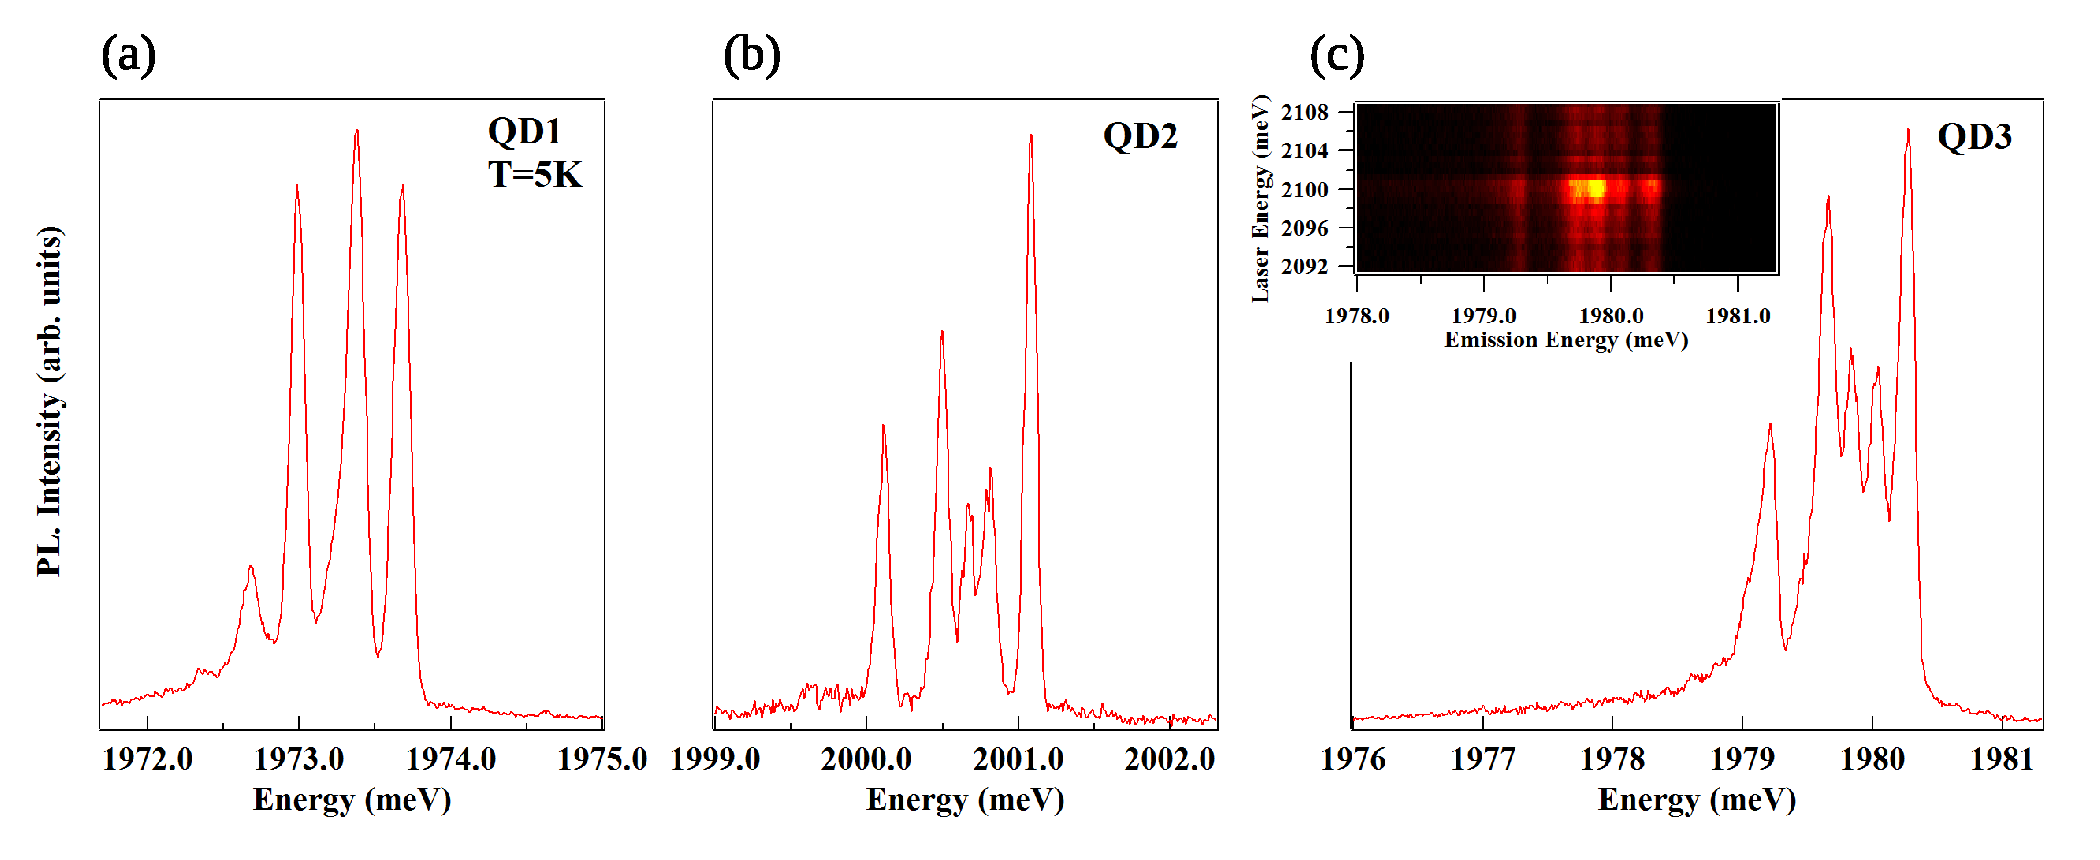
\includegraphics[width=15cm]{04-CrMagOpt/Pictures/Spectras.eps}
	\end{center}
	\caption{PL of X-Cr complex at low temperature (T=5K) for (a) QD1 (found in dot334), (b) QD2 (dot338) and (c) QD3 (dot334). Inset in (c) presents the PLE map of this QD, showing a sharp quasi-resonant state for an excitation at 2100 meV.}
	\label{SpectraX}
	\end{figure}

	Low temperature (T=5K) PL of the neutral exciton (X-Cr) of several QDs doped with a single Cr are reported in Fig.~\ref{SpectraX}. Three main emission lines are observed, with a fourth, weaker peak on the low energy side. In some QDs, such as QD2 and QD3, the central peak is split. Scanning with an energy tunable laser, we saw that all the peaks share a common excited state, as highlighted in the inset of Fig.~\ref{SpectraX}(c). This is an indication that they originate from the same dot. Variations in the relative intensities of the peaks are observed from dots to dots.

	\begin{figure}[h!]
	\begin{center}
		\includegraphics[width=10cm]{04-CrMagOpt/Pictures/EnLvlantiferro.png}
	\end{center}
	\caption{Illustration of the energy levels of the ground state (Cr), the bright exciton states ($|\pm1\rangle$) coupled to the spin of a Cr (X-Cr) and dominant PL transitions ($\sigma$+, $\sigma$-). The states $S_z = \pm2$ cannot be populated through thermalization, and thus their recombination channel are not shown on this schema.}
	\label{CrEnergyStruct}
	\end{figure}

	As we have seen in Sec.~\ref{CrSemiCon}, in a II-VI semiconductor, the orbital momentum of the Cr connects the spin of the atom to its local strain environment through the modification of the crystal field and the spin-orbit coupling. For biaxial strain in the (001) plane, the ground state of a Cr spin is split by a strain induced magnetic anisotropy term ${\cal H}_{Cr,\varepsilon_\parallel}=D_0S^2_z$. It was deduced from electron paramagnetic resonance of bulk Cr-doped CdTe that $D_0$ is positive for compressive biaxial strain~\cite{EPRCr}. In a self-assembled CdTe/ZnTe QDs with large in-plane strain, the Cr spin energy levels are split from $|S_z=0\rangle$ (Fig.~\ref{CrEnergyStruct}). A value of $D_0$ in the meV range can be expected for a CdTe layer strained on a ZnTe substrate, as shown in Sec.~\ref{CrSemiCon}.
	
	\begin{figure}[h!]
	\begin{center}
		\includegraphics[width=15cm]{04-CrMagOpt/Pictures/LinPol.png}
	\end{center}
	\caption{(a) Low temperature (T = 5 K) PL of QD2 recorded in linear polarization along two orthogonal directions. (b) Linear polarization PL intensity map of QD2. The 0$^{\circ}$ polarization angle corresponds to an emission polarized along the QD cleavage axis, either $[110]$ or $[1\bar{1}0]$. (c) Illustration of the energy levels of the ground state (Cr), the bright exciton states ($|\pm1\rangle$) coupled to the spin of a Cr (X-Cr), showing the splitting of the central peak via the bright exciton coupling, and dominant PL transitions: $\sigma$+ in blue, $\sigma-$ in red and $\pi$ in green and black.}
	\label{CrLinPolar}
	\end{figure}
	
	When an electron-hole pair is injected in a Cr-doped QD, the bright excitons are split by the exchange interaction between the spins of Cr and carriers. In flat self-assembled QDs, the heavy-holes and light-holes are separated in energy by the biaxial strain and the confinement. In a first approximation, the ground state in such QD is a pure heavy-hole ($J_z$=$\pm$3/2) exciton and the exchange interaction with the Cr spin S is described by the spin Hamiltonian 
	\begin{align}
		{\cal H}_{c-Cr}=I_{eCr}\mathbf{S}\cdot\bm{\upsigma}+I_{hCr}S_zJ_z
	\end{align}		
with $\bm{\upsigma}$ the electron spin and $J_z$ the hole spin operator. $I_{eCr}$ and $I_{hCr}$ are, respectively, the exchange integrals of the electron and the hole spins with the Cr spin. These exchange energies depend on the exchange constant of the Cr $3d$ electrons with the CdTe carriers and on the overlap of the Cr atom with the confined carriers. Even though the exchange interaction of the Cr spin with both electron and hole is ferromagnetic in most II-VI semiconductor~\cite{MacCdCrSD0beta,KacmanD0alphabetaIIVI,MacspdexchCr}, the hole-Cr interaction is supposed to be anti-ferromagnetic here. This does not change the structure of the PL at B = 0T. The only visible effect will be on the PL intensity distribution in the magneto-optics experiments. This choice of sign of the hole-Cr exchange interaction will be further discussed in Sec.~\ref{MagOptCr}. A typical exchange constant 4 to 5 times larger for the holes than for the electrons is also expected in CdTe~\cite{DMSCrExchInt,CdCrSExchInt}.

	\begin{figure}[h!]
	\begin{center}
		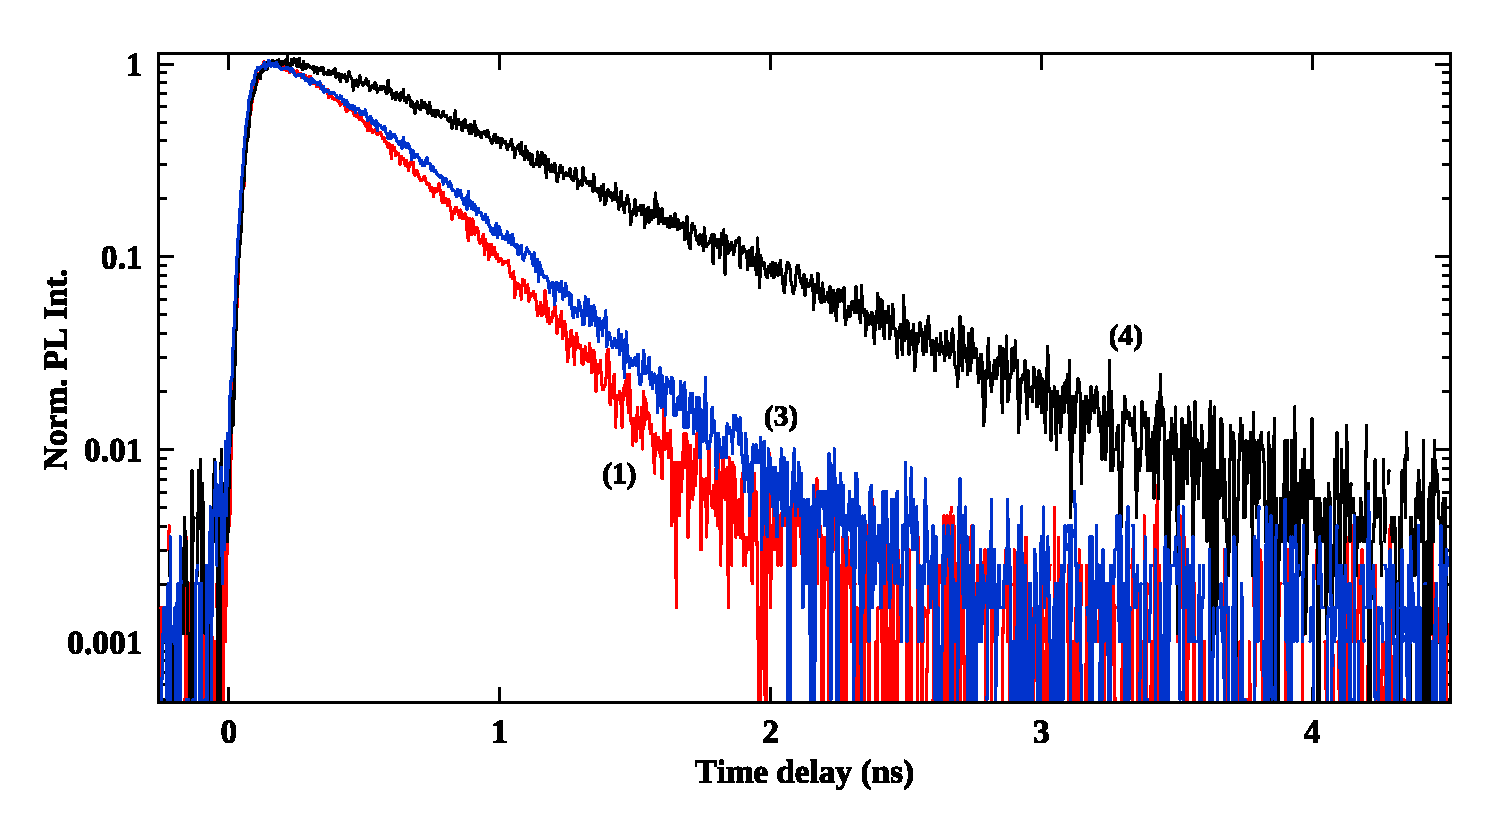
\includegraphics[width=12cm]{04-CrMagOpt/Pictures/Decay.eps}
	\end{center}
	\caption{Time resolved PL of QD2 taken on two outside peaks at T = 5 K, attributed to $S_z = \pm1$ (noted (1) and (3) in Fig.~\ref{CrLinPolar}(a)), and the lower energy one (noted (4)).}
	\label{CrDecay}
	\end{figure}
	
	For highly strained CdTe/ZnTe QDs with a weak hole confinement, the strain induced energy splitting of the Cr spin $D_0S^2_z$ is much larger than the exchange energy with the confined carriers ($D_0\gg |I_{hCr}|>|I_{eCr}|$). The exchange interaction with the exciton acts as an effective magnetic field which further splits the Cr spins states $S_z=\pm$1 and $S_z=\pm$2. The resulting X-Cr energy levels are presented in Fig.~\ref{CrEnergyStruct}. The exciton recombination does not affect the Cr atom and its spin is conserved during the optical transitions. Consequently, the large strain induced splitting of the Cr spin is not directly observed in the optical spectra. However, at low temperature, the Cr spin thermalize on the low energy states $S_z$=0 and $S_z$=$\pm$1. This leads to a PL dominated by three contributions: a central line corresponding to $S_z=0$ and the two outer lines associated with $S_z=\pm$1 split by the exchange interaction with the carriers.
	
	Cr-doped quantum dots exhibit a linear polarization dependence, as presented in Fig.~\ref{CrLinPolar}. The central line ($S_z$=0) is split and linearly polarized along two orthogonal directions. As in non-magnetic QDs, this results from a coupling of the two bright excitons $|\pm1\rangle$ by (i) the long-range e-h exchange interaction in a QD with an in-plane shape anisotropy~\cite{SplitInvTh} and/or (ii) the short range e-h exchange interaction in the presence of valence band mixing. This anisotropic e-h exchange energy mixes the bright exciton associated with the same Cr spin state, inducing an extra splitting between them. The mixing is maximum for the central pair of bright excitons (S$_z$=0) which are initially degenerated. The outer lines are also slightly linearly polarized but the influence of the e-h exchange interaction is attenuated by the initial splitting of the $|\pm1\rangle$ excitons induced by the exchange interaction with the Cr spin $S_z=\pm1$.	

	In order to identify the nature of the lower energy peak ((4) in Fig.~\ref{CrLinPolar}(a)), we performed time resolved PL experiments on the emission peaks (1), (3) and (4). The results, presented in Fig.~\ref{CrDecay}, show that the line (4) presents a decay time about twice longer than the other lines. Such a long decay time is consistent with the radiative recombination of a dark exciton. Under normal circumstances, the recombination of such a state is forbidden. However, it is possible to observe a dark exciton emitting a photon in low symmetry QDs~\cite{DELum}. Since it is initially a forbidden transition, the recombination will be less efficient and will thus take more time~\cite{DELongLifetime}. This hypothesis will be confirmed by the magneto-optical study of the dot presented in Fig.~\ref{CrMagOptExp} and \ref{CrMagOptMod}.
	
	\begin{figure}[h!]
	\begin{center}
		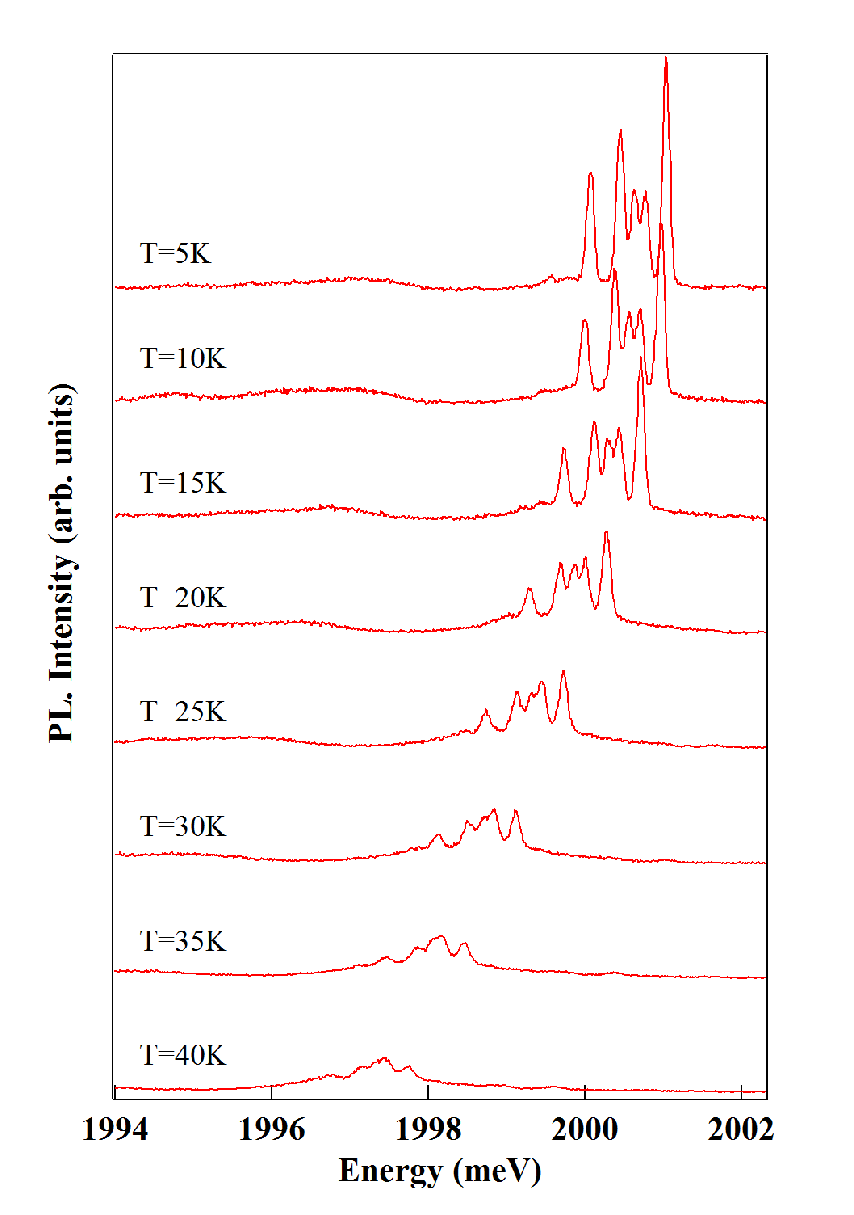
\includegraphics[width=14.9cm]{04-CrMagOpt/Pictures/Temp.eps}
	\end{center}
	\caption{Temperature evolution from T=5K to T=40K of (a) the PL of QD2 and (b) the PL of a QD with a good thermalisation on the low energy states (QD4).}
	\label{CrTemp}
	\end{figure}
	
	Since the Cr spin states $S_z = \pm2$ do not appear on the PL because they cannot be thermally populated at T = 5K, one could expect to see their emission at higher temperature. Fig.~\ref{CrTemp} presents the emission of two dots as a function of the temperature. With the increase of the temperature, we observe a significant line broadening induced by the interaction with acoustic phonons~\cite{BesombesAccPhon}. In order to keep a significant PL intensity and resolved PL lines, we limited our investigation to temperature below 40K. Even at this temperature, the PL peaks corresponding to $S_z = \pm2$ does not appear. However, the structure of the emission change slightly with the temperature. The intensity of the outside peaks, associated with the states $S_z = \pm1$, decreases faster than the intensity of the PL peak associated with $S_z = 0$ when the temperature increases. This is an unexpected picture, since a higher temperature should allow the higher energy states $S_z = \pm1$ to be more populated by emptying the ground state when increasing. To explain this behaviour on the low energy peak, we propose that the state $S_z = 0$ is partly populated by a h-Cr spins flip-flop from the states $S-z = \pm1$ coupled to the dark states. This process is explained with more details in Sec.~V.3.1%~\ref{hCrff}
. When the temperature rises, the probability for the dark states to recombine non-radiatively increases, and thus the decrease of the population and PL intensity of the peaks associated with the state $S_z = 0$ would be slower than the intensity of the one associated with $S_z = \pm1$.
	%\newpage


		\subsection{Excited states of a Cr-doped QD}	
	
	The excited states in QD2 were investigated by PLE, starting close to the energy of the dot's emission. The data reported in Fig.~\ref{FullPLE}(a) present several excited states at different excitation energy.
	
	\begin{figure}[h!]
	\begin{center}
		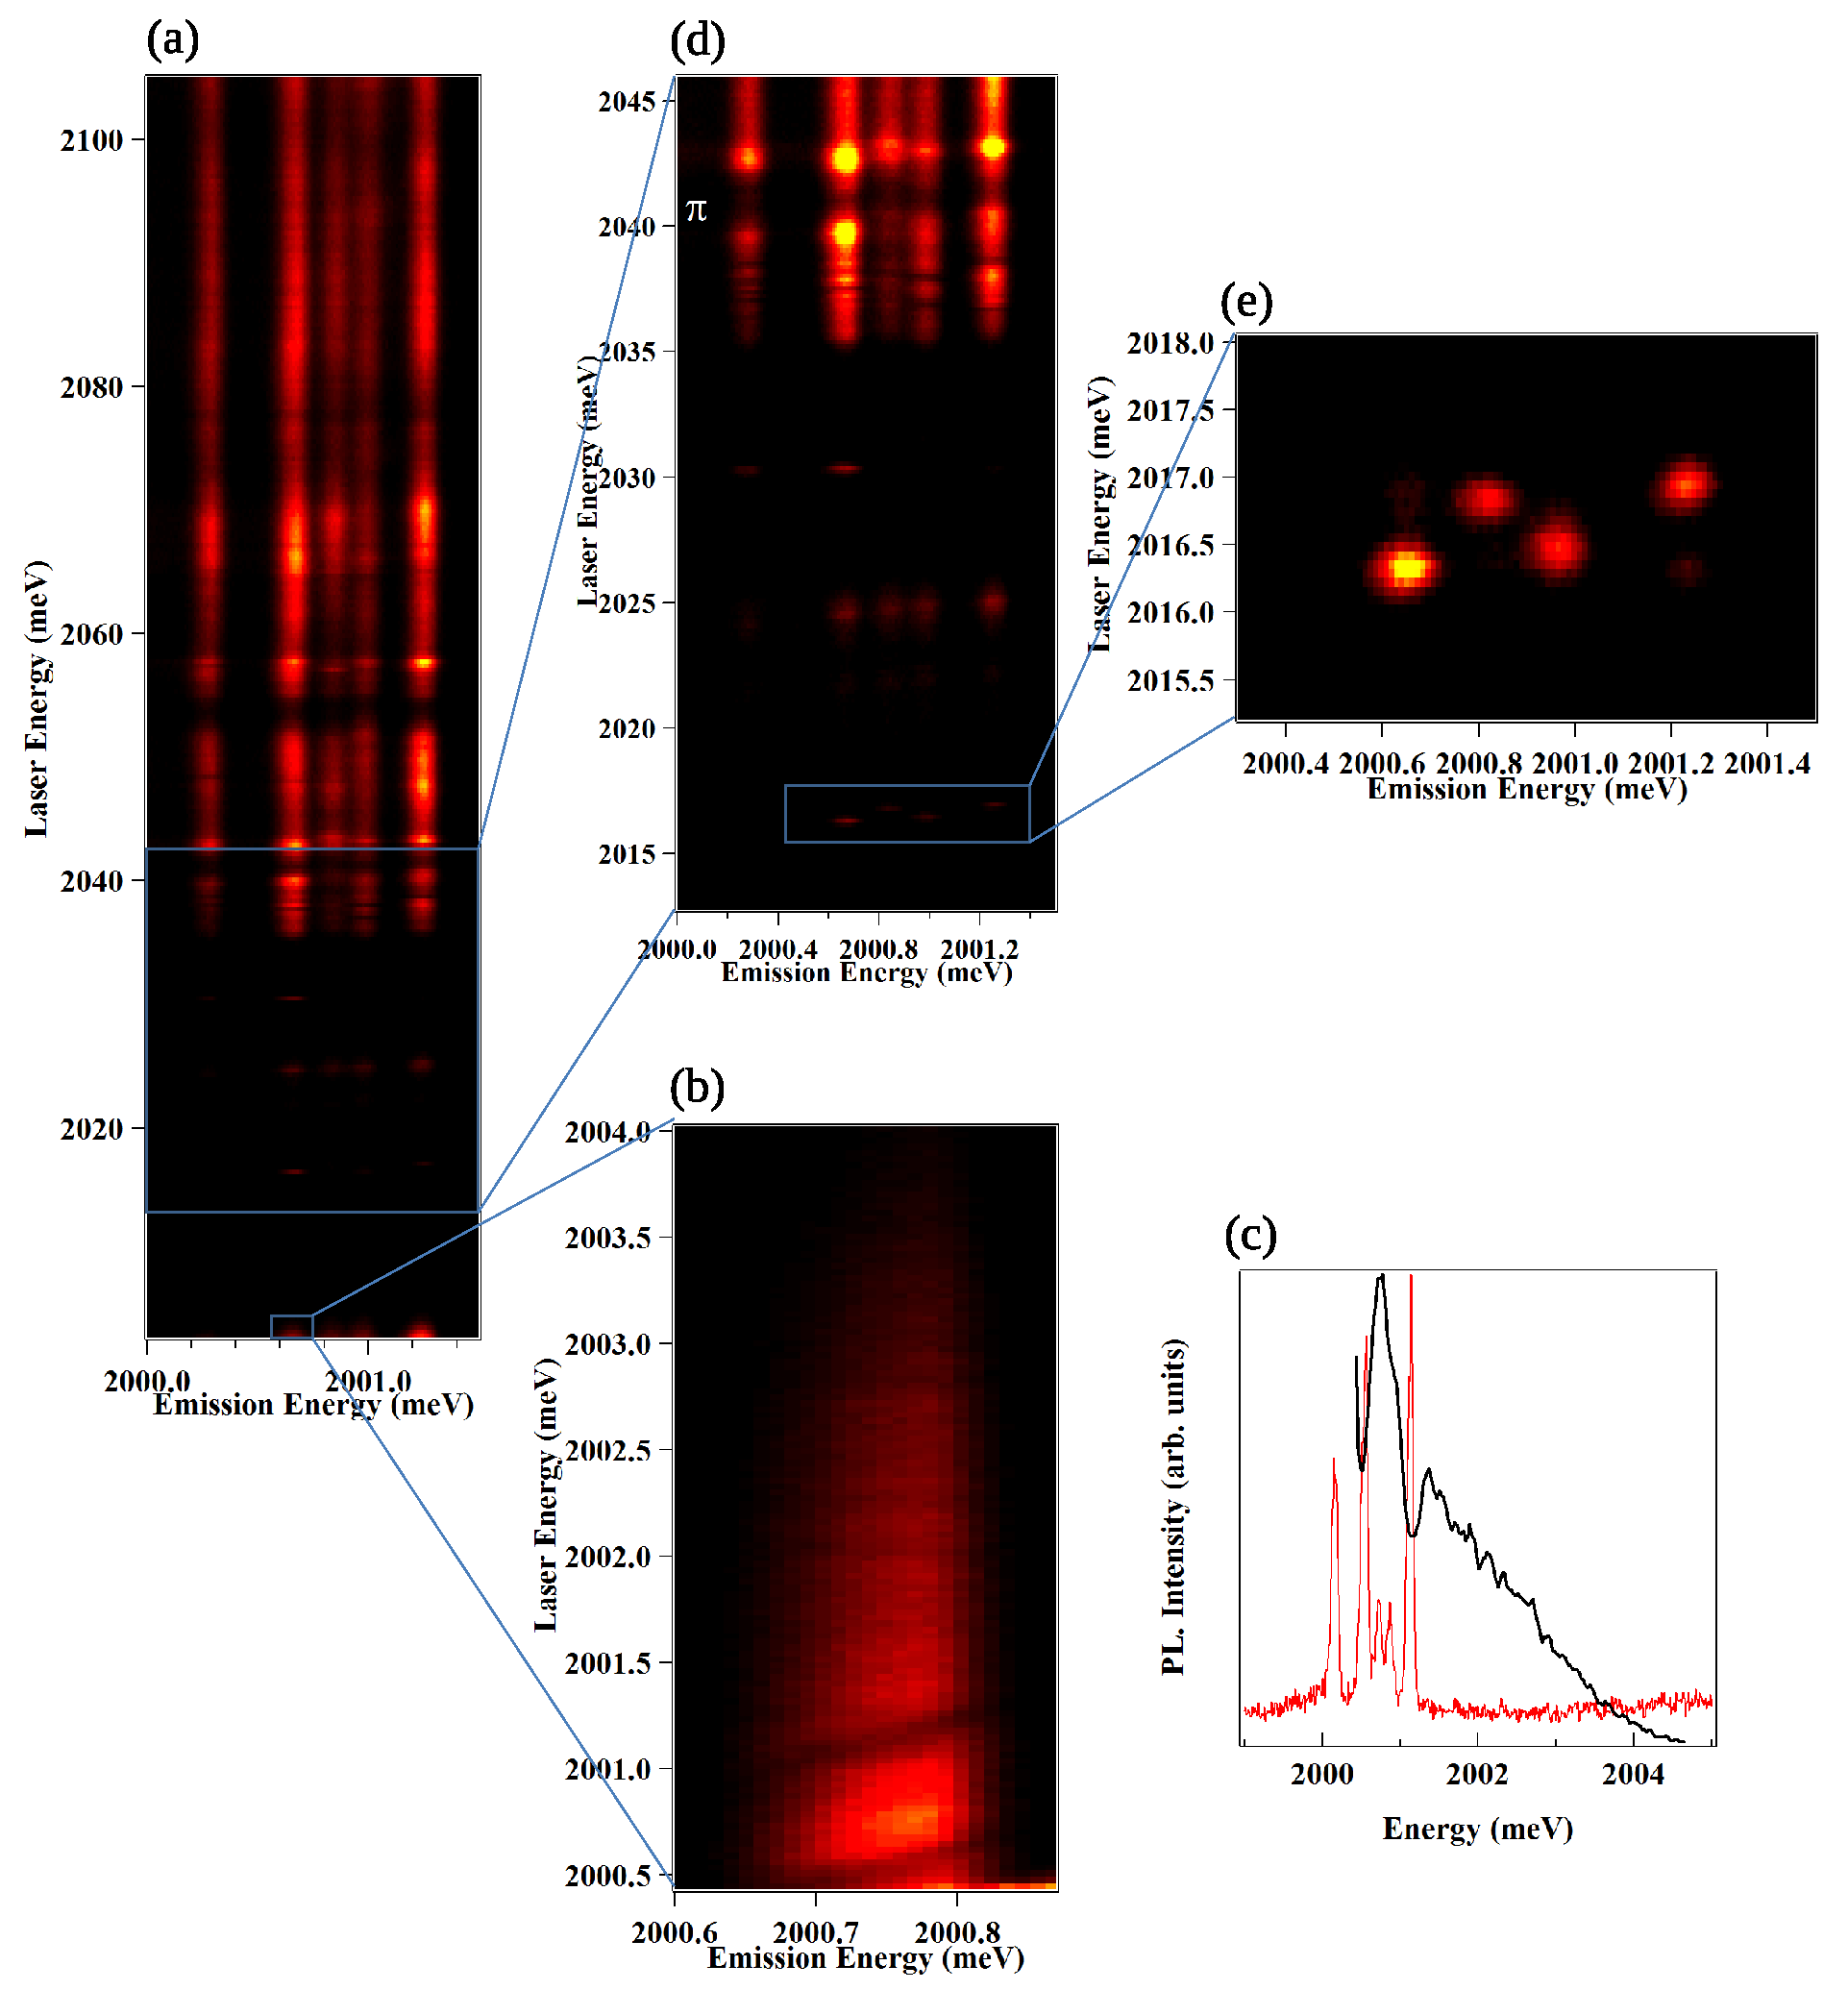
\includegraphics[width=13.8cm]{04-CrMagOpt/Pictures/FullPLEv2.eps}
	\end{center}
	\caption{(a) QD2 X-Cr PLE map at T = 5 K in $\pi_{cross}$ polarization. Several excited states are highlighted. (b) Photoluminescence of QD2 X-Cr complex for an excitation at 2120 meV). (c) PLE scan detected on the lower energy peak, taken close to the QD emission energy, showing the phonon replica taken in $\pi$ detection. The emission integrated intensity in function of the laser energy is plotted in (d) (black curve) along with the PL spectra of QD2 taken in $\sigma_{co}$ polarization. (e) PLE map between 2046 meV and 2013 meV presenting several excited, detecting in $\pi_{cross}$ polarization. (f) Zoom in a particular excited state presented a splitting inversion, taken in $\pi_{cross}$ detection.}
	\label{FullPLE}
	\end{figure}
	
	Starting at low excitation energy, the first noticeable thing on this scan is the PL observed over a large excitation energy range, for an excitation between the dot emission energy (between 2000 and 2001 meV) and 2004 meV. A zoom is presented in Fig.~\ref{FullPLE} (c) for a detection on the dark exciton line. This corresponds to an excitation of the QD via the acoustic phonon band. 
One can notice two sharp intensity decreases in this emission. Comparing the integrated intensity of the PL of the dark state during the laser scan with the QD spectra (Fig.~\ref{FullPLE}(d)), it appears that those two intensity drops happen when the laser is in resonance with a QD emission line. At the resonance, the absorption preferentially occurs in this resonantly excited state than in the acoustic phonon band of the low energy line.

	
	Another excited state appears around 2018.5 meV, zoomed in on Fig.~\ref{FullPLE} (f). The first feature of this peak is that, each of the peak here presents a slightly different resonant energy. Moreover, one can note that the order of appearance during the energy scan of the two central peaks seems to be reversed compared to the external ones. For the outside peaks, the low energy one appears before the high energy one. This order is inverted for the central peaks. Such splitting inversion, was first observed on QDs in GaAs quantum well~\cite{FineStructSplitGaAsdots}. It has been discussed by Takagahara~\cite{SplitInvTh} and is due to the electron-hole exchange interaction in anisotropic potential.
	
	\begin{figure}[h!]
	\begin{center}
		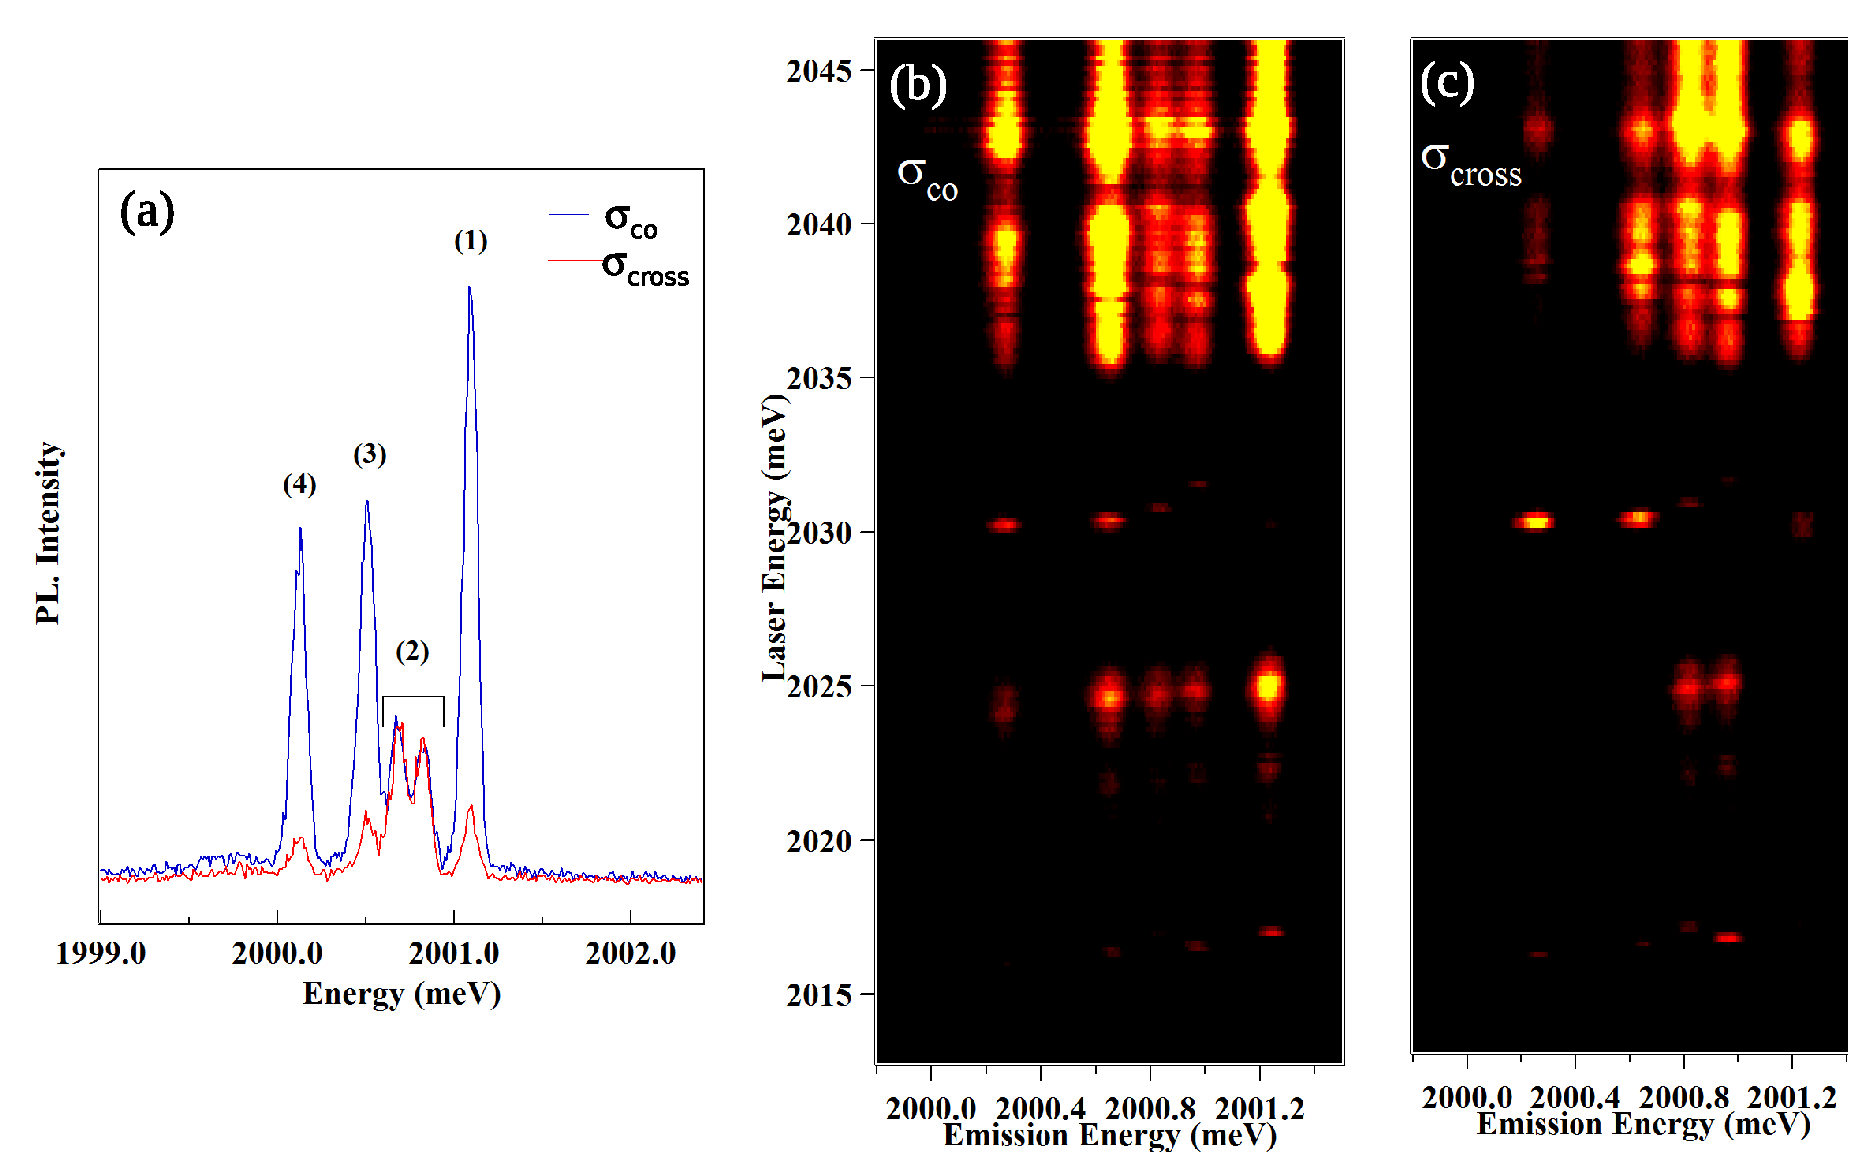
\includegraphics[width=14.9cm]{04-CrMagOpt/Pictures/PLEDotPres.eps}
	\end{center}
	\caption{(a) Low temperature (T = 5 K) PL spectra of the exciton in QD2 (X-Cr) for co-circularly (blue) and cross-circularly (red) polarized excitation/detection taken for an excitation around 2120 meV. (b) - (c) PLE map at T = 5 K between 2046 meV and 2013 meV presenting several excited states, detected in $\sigma_{co}$ (b) and $\sigma_{cross}$ (c).}
	\label{PLEDotPres}
	\end{figure}
	
	The next excited state can be seen at 2025 meV, more visible on ~\ref{FullPLE} (e). It can be linked to an excitation through optical phonons. Looking at the $\sigma$ polarized emissions for an excitation on these states (Fig.~\ref{PLEDotPres}(b) and (c)), we can see that the low and high energy peaks are strongly $\sigma_{co}$ polarized. It means that the exciton recombines in the same spin as the one injected by the laser. It shows that the spin of the exciton in the QD is conserved during its lifetime. This stabilization of the exciton spin is due to the Cr spin acting as an effective magnetic field. The splitting of the central peak, shown in Fig.~\ref{PLEDotPres}, is linearly polarized, as discussed in Sec.~\ref{CrPres}: as expected, its emission shows no dependency in circular polarization. 
	
	Finally, another interesting excited state appear at 2030 meV. This state presents a different exchange-induced splitting than the splitting in the excited state around 2100 meV presented in Fig.~\ref{SpectraX}. This is due to a difference in the carriers and Cr atom wavefunction overlap.

		\subsection{Magneto-optics of QDs doped with a single Cr atom\label{MagOptCr}}
		
	The structure of the energy levels of Cr-doped QDs presented in Fig.~\ref{CrEnergyStruct} is confirmed by the evolution of the PL spectra in magnetic field, up to 11 T, along the growth axis, the so called Faraday configuration~\cite{BesombesPumpMnSFD}, presented in Fig.~\ref{CrMagOptExp}. When applying such a magnetic field, the bright exciton $X_z = \pm1$ splits, leading to a $\sigma-$ branch shifting at low energy and a $\sigma+$ one shifting at high energy. This splitting can compensate the one induced by the exchange interaction with the Cr~\cite{LegerQDGeomEffect}. For QD1, this results in an anti-crossing of $|+1\rangle$ and $|-1\rangle$ excitons due to the e-h exchange interaction around B$_z$=6 T observed both in $\sigma+$ and $\sigma-$ polarizations (anti-crossing (2) and (3) in Fig.~\ref{CrMagOptExp}(a)).
		
	\begin{figure}[h!]
	\begin{center}
		\includegraphics[width=10cm]{04-CrMagOpt/Pictures/MagOptv2.png}
	\end{center}
	\caption{(a) Evolution of the circularly polarized X-Cr PL of QD1 under magnetic field applied along the growth axis ($B_z$) at T = 5 K. ASee text for the identification of the anti-crossing (1), (2), (3) and (4). (b) Corresponding PL spectra taken at 0 and $10$T for both circular polarization.}
	\label{CrMagOptExp}
	\end{figure}
		
		The low energy emission presented as a dark exciton in Fig.~\ref{CrDecay} shows an anti-crossing with the bright excitons under $B_z$ in $\sigma-$ polarization (anti-crossing (4) in Fig.~\ref{CrMagOptExp}). This anti-crossing arises from a mixing of the bright and dark excitons interacting with the same Cr spin state. When detecting in $\sigma-$ polarization, it corresponds to the mixing of the exciton states $|-1\rangle$ and $|+2\rangle$ coupled to the Cr spin $S_z=+1$. This dark/bright excitons coupling $\delta_{12}$ is induced by the e-h exchange interaction in a confining potential with a symmetry lower than C$_{2v}$~\cite{DERecombTh}. In such symmetry, the dark exciton acquire an in-plane dipole moment which leads to possible optical recombination at zero magnetic field~\cite{DELum}. The oscillator strength of this "dark exciton" increases as the initial splitting between $|-1\rangle$ and $|+2\rangle$ excitons is reduced by the magnetic field.
		
	\begin{figure}[h!]
	\begin{center}
		\includegraphics[width=10cm]{04-CrMagOpt/Pictures/MagOptLowSym.eps}
	\end{center}
	\caption{Linear polarization intensity map (a) X$^2$-Cr and (c) X-Cr in QD3. (b) - (d) Respective intensity map of the longitudinal magnetic field dependence of the emission (bottom panel) of }
	\label{CrMagOptLowSym}
	\end{figure}
		
		To illustrate the influence of the QD symmetry on the magneto-optical properties of X-Cr, we show in Fig.~\ref{CrMagOptLowSym}(b) the emission of a QD with a different strain or shape anisotropy (QD3). For QD1, the splitting of the central peak is not clear in the PL at 0T (Fig.~\ref{SpectraX}(a)), while two linearly polarized peaks appear in QD3 spectra (Fig.~\ref{SpectraX}(c)).
		
		Investigating both the biexciton and the exciton in the same Cr-doped QD, we can also analyze the impact of the carrier-Cr interaction on the fine structure of the Cr spin. The magnetic field dependence of X$^2$-Cr emission in QD3 is presented along with the X-Cr emission as a contour plot in Fig.~\ref{CrMagOptLowSym} (a) and (b) respectively. The PLs under magnetic field of X-Cr and X$^2$-Cr present a mirror symmetry. In particular, the dark/bright exciton mixing observed around $B_z=2.5$ T on the low energy side of the PL in $\sigma-$ polarization for X-Cr is observed on the high energy side in $\sigma+$ polarization for X$^2$-Cr (circles in Fig.~\ref{CrMagOptLowSym}(a) and (b)).
		
	\begin{figure}[h!]
	\begin{center}
		\includegraphics[width=13cm]{04-CrMagOpt/Pictures/Antiferro-Cr.png}
	\end{center}
	\caption{(a) Evolution in magnetic field of QD4 X-Cr circularly polarized PL. (b) QD3 X-Cr PL at $B_z = 0$ T and $B_z = 7$ T in both polarization. A schema presenting the spin configuration for the most intense outer peak under magnetic field is joined on the side.}
	\label{CrAntiferro}
	\end{figure}
		
		If one considers the ground state of X$^2$ as a spin-singlet (total spin 0), it cannot be split by the magnetic field or the spin interaction part of the carriers-Cr hamiltonian. The creation of two excitons in the QD cancels the exchange interaction with the Cr atom. Thus, the PL of  X$^2$-Cr is controlled by the final state of the optical transitions, i.e. the eigenstates of X-Cr, resulting in the observed mirror symmetry in the PL spectra.
		
	\begin{figure}[h!]
	\begin{center}
		\includegraphics[width=10cm]{04-CrMagOpt/Pictures/Antiferro-Mn.eps}
	\end{center}
	\caption{(a) Evolution in magnetic field of the PL of a single Manganese atom coupled to an exciton in a II-VI QD. (b) PL spectra of the X-Mn system taken at $B_z = 0$ T and $B_z = 11$ T in both circular polarization. These experimental results are taken from Yoan L\'eger PhD thesis~\cite{YoanTh}.}
	\label{MnAntiferro}
	\end{figure}
		
	The sign of the interaction between the Cr and the hole spin can be found by studying the evolution under magnetic field of the relative intensity of each of the QD peaks. As shown in Fig.~\ref{CrEnergyStruct}, for a given polarization, each peak can be linked to a Cr spin state. As discussed earlier, applying a magnetic field lifts the degeneracy between the exciton states and allows to efficiently select the polarization of the emission. In Cr-doped QDs, the evolution of the peaks relative intensities under magnetic field is consistent with an anti-ferromagnetic h-Cr exchange interaction.
	
	QD4, shown in Fig.~\ref{CrAntiferro}, presents a high contrast in the evolution of the intensity under magnetic field and was used to find the sign of the h-Cr exchange interaction. The central peak intensity stays the stronger of the three peaks, whatever the direction of the magnetic field. This is expected, since the $S_z = 0$ state is not affected by the Zeeman effect. It remains the lower spin state for the Cr atom, and therefore concentrate most of the population. In the $\sigma-$ branch, the high energy peak get brighter while the low energy one disappears for $B_z \geq 8$T in QD4. The situation is opposite in the $\sigma+$ branch, where the intensity concentrate on the lower energy peak associated with a bright exciton state.
	
	We will focus in this analysis on the Cr spin states $S_z = \pm1$, associated with the two outside peaks. Under magnetic field, $S_z = -1$ shifts at lower energy, while $S_z = +1$ shufts at higher energy, due to the Zeeman effect. Therefore, at high enough magnetic field, the recombination occurs mainly toward $S_z = -1$. In $\sigma-$ polarization, the PL intensity concentrate on the high energy peak. Since we selectively inject $X_z = -1$ excitons, the high energy state is $|S_z = -1, X_z = -1\rangle$. The same analysis can be done for an excitation in $\sigma+$ polarization: the injected exciton has an angular momentum $X_z = +1$ and the lower energy line is the most intense. It means the $|S_z = -1, X_z = +1\rangle$ state is at low energy. 

	This situation is similar to the one observed in II-VI QDs doped by a single Mn atom, presented in Fig.~\ref{MnAntiferro}. Mn is known to have an anti-ferromagnetic interaction with the hole in CdTe~\cite{GajMnD0alphabeta}. It was shown in \cite{YoanTh} that, under magnetic field, the intensity was mainly on the high energy side when injecting $X_z = -1$ excitons, and on the low energy side when injecting $X_z = +1$ excitons.
	%The $S_z = -\frac{5}{2}$ state of the Mn atom was stabilized under magnetic field. From the evolution of the peaks relative intensity and the polarization of the different Mn states, it was then possible to deduce that the interaction between Mn and hole was anti-ferromagnetic.

	The same evolution was found in our other QDs. All of this shows that hole-Cr exchange interaction is an anti-ferromagnetic in self-assembled QDs. This interaction varies dramatically with the environment: it can go from ferromagnetic to anti-ferromagnetic in a strained environment, as was discussed in Sec.~\ref{CrCdTe}. It also confirms the energy structure presented in Fig.~\ref{CrEnergyStruct}.
		
	\section{Modelization of a Cr-doped QD\label{QDParam}}
	
	The system can be described by a spin effective hamiltonian, that we separate as follows:
	
	\begin{align}
\label{X-Cr} {\cal H}_{X-Cr}={\cal H}_{Cr,\varepsilon}+{\cal H}_{cCr}+{\cal H}_{mag}+{\cal H}_{eh}+{\cal H}_{band}+{\cal H}_{scat}
	\end{align}
where:

${\cal H}_{Cr,\varepsilon}$ describes the fine structure of the Cr atom and its dependency on local strain, as presented in Eq.~\ref{Cralone}. It is mainly drived by $D_0$, the magnetic anisotropy. The in-plane strain anisotropy $E$ has to be small (in the meV range) in order for model to reproduce well the data (see Fig.~\ref{CrHighE} for the emission of a dot with a higher E).

\begin{figure}[h!]
	\begin{center}
		\includegraphics[width=14.9cm]{04-CrMagOpt/Pictures/SimuAntiferro.png}
	\end{center}
	\caption{(a) Calculated linear polarization PL intensity map of X-Cr at zero field. The 0$^{\circ}$ polarization angle correspond to an emission polarized along the $[100]$ axis. (b) Right: Calculated magnetic field dependency of X-Cr circularly polarized PL. See text for details of the model. Parameters are listed in Tab.~\ref{CrModelParam}. Corresponding anti-crossing are highlighted in the same fashion as on Fig.~\ref{CrMagOptExp} and \ref{CrAntiferro}. Left: PL spectra calculated for $B_z = 0$ T and $B_z = 11$ T in both circular polarization. The peaks intensity was calculated using only a thermal distribution. (c) Schema of the magnetic field dependency of the energy levels of the low energy Cr spin states $S_z$=0 and $S_z$=$\pm$1, and corresponding bright ($+1$ blue, $-1$ red) and dark ($|\pm2\rangle$ green) X-Cr energy levels.}
	\label{CrMagOptMod}
	\end{figure}

${\cal H}_{cCr}$ describes the coupling of the electron and hole with the Cr spin, depending on $I_{eCr}$, the exchange integral of the electron-Cr spins, and $I_{hCr}$, the exchange integral of the hole-Cr spins, as described in Eq.~\ref{HCrDMS}.

${\cal H}_{mag}$ describes the effect of a magnetic field, coupled to both the Cr and carrier spins by the Zeeman terms, depending on the $g$-factor of each of them and the Bohr magneton $\mu_B$, and including the diamagnetic shift of the electron-hole via the term $\gamma$:
\begin{align}
	{\cal H}_{mag} = g_{Cr}\mu_B\overrightarrow{B}.\overrightarrow{S}+g_{e}\mu_B\overrightarrow{B}.\overrightarrow{\sigma}+g_{h}\mu_B\overrightarrow{B}.\overrightarrow{J}+\gamma B^2
\end{align}

${\cal H}_{eh}$ describes the short range and long range electron-hole interaction, through the bright and dark exciton splitting $\delta_0$, the bright exciton coupling $\delta_1$, the dark exciton coupling $\delta_2$ and the bright and dark exciton coupling $\delta_{11}$ and $\delta_{12}$. All of these term are described in Eq.~\ref{HehCs}.

${\cal H}_{band}$ is the band Hamiltonian. It is written ${\cal H}_{band} = E_g + {\cal H}_{VBM}$, with $E_g$ the band gap of CdTe and ${\cal H}_{VBM}$ the valence band mixing, described in Eq.~\ref{HVBM}.

${\cal H}_{scat}$ describes the perturbation of the wave function of the exciton in the initial state of the optical transition by the hole-Cr exchange interaction, controlled by the parameter $\eta$. It was described in Sec.~\ref{hMnSpinStruct}. It can be written using the second order perturbation theory by an effective spin hamiltonian:
\begin{align}
{\cal H}_{scat}=-\eta S_z^2
\end{align}
\noindent with $\eta>0$.

	We considered the general case of QDs with a symmetry lower than C$_{2v}$ (truncated ellipsoidal lens for example~\cite{DERecombTh}), and took into account the influence of this reduced symmetry on the valence band and on the e-h exchange interaction. The population of the X-Cr spin states splits by the large magnetic anisotropy and the carriers-Cr exchange interaction is described by a spin effective temperature $T_{eff}$, applied on the X-Cr levels. The results of the model obtained with $T_{eff}=20$ K, $D_0=2.2$ meV and an electron-Cr (hole-Cr) exchange interaction $I_{eCr}=-50$ $\mu$eV ($I_{hCr}=250$ $\mu$eV) are reported in Fig.~\ref{CrMagOptMod}. The parameters not specific to Cr-doped QDs are listed in Tab.~\ref{CrModelParam}. Such parameters do not aim to precisely fit the data and are only reasonable order of magnitude to qualitatively reproduce the experimental results of the PL of X-Cr at zero field and its evolution in magnetic field. The splitting of the central line at zero field (anti-crossing (1)) and the anti-crossings under magnetic field (anti-crossings (2) and (3) around $B_z$=6T for the Cr spin states  $S_z = |+1\rangle$ and anti-crossings (4) with the dark exciton around $B_z$=2T) are well reproduced by the model.
	
	This model also predicts an anti-crossing around $B_z = 5$ T, noted (5), caused by an electron-Cr flip flop, which is not seen in the experiments. Its position is controlled by $D_0$ and its intensity by $I_{eCr}$. If $D_0 > 3$ meV, the anti-crossing (5) appears for $B_z > 11$ T, outside of our magnetic field range ($-11$ T $< B_z < +11$ T). However, such a high value of $D_0$ would put the Cr spin state $S_z = \pm1$ at high energy, increasing the population of $S_z = 0$. This would lead to a higher PL intensity of the central peak, associated with $S_z = 0$, than observed experimentally. Therefore, a low value of $I_{eCr}$ was chosen instead, to reduce the anti-crossing intensity.
	
	Finally, the remaining tail of an anti-crossing, labelled (6), also appears at high magnetic field in the $\sigma-$ polarization, as seen in Fig.~\ref{CrAntiferro}, due to the coupling a bright and a dark exciton coupled to the Cr state $S_z = 0$.

	


\begin{table}[t] \centering
	\caption{Values of the parameters used in the model of Cr-doped CdTe/ZnTe quantum dot presented in Fig.~\ref{CrMagOptMod}. The value of the parameters not listed in the table is 0. The chosen values are typical for CdTe/ZnTe quantum dots and can be compared with parameters extracted from Mn-doped quantum dots \cite{DynhMn,DELum}. These values are reasonable to reproduce the emission of the QDs presented in this thesis.}
	\begin{tabular}{p{0.9cm}p{0.9cm}p{0.9cm}p{0.9cm}p{0.9cm}p{0.9cm}p{0.9cm}p{0.9cm}}
\hline\hline
I$_{eCr}$ & I$_{hCr}$ & $\delta_0$ & $\delta_1$ & $\delta_{12}$ & $\delta_{11}$ & $\frac{|s|}{\Delta_{lh}}$ & $\frac{|r|}{\Delta_{lh}}$ \\
$\mu eV$ & $\mu eV$ & $meV$ & $\mu eV$ & $\mu eV$ & $\mu eV$ &  & \\
\hline
-50 & 250 & -1 & 250 & 150 & 50 & 0.05 & 0.05 \\
\hline\hline 
	\end{tabular}
	\begin{tabular}{p{0.9cm}p{0.9cm}p{0.9cm}p{0.9cm}p{0.9cm}p{1.3cm}p{0.9cm}p{0.9cm}}
arg(r) & $D_0$ & $g_{Cr}$ & $g_{e}$ & $g_{h}$ & $\gamma$ & $\eta$ & $T_{eff}$ \\
 & $meV$ & &  &  & $\mu eV/T^2$ & $\mu eV$ & K \\
\hline
$-\dfrac{\pi}{2}$ & 2.2 & 2 & -1 & 0.4 & 1.5 & 25 & 20 \\
\hline\hline
	\end{tabular}
	\label{CrModelParam}
	\end{table}
	
	The magnetic anisotropy $D_0$ cannot be precisely extracted from the PL spectra. However, for $D_0 <  2$ meV, an anti-crossing due to a VBM induced hole-Cr flip-flop between the $|-1, +2\rangle$ and the $|0, -1\rangle$ would appear for $B_z < 11$ T on the central line in $\sigma-$ polarization. Moreover, as discussed earlier, a $D_0 > 3$ meV would produce a lower PL intensity for the states $S_z = \pm1$. These considerations set $D_0$ in the range of 2 to 3 meV. However, even in this range, the intensity distribution of the PL cannot be perfectly reproduced: while the evolution under magnetic field of the intensity ratio of the peaks is quite well predicted for high value of the magnetic field, the $S_z = 0$ state still presents a stronger emission at $B_z = 0$ T than the one observed in the experiments. This difference may be due to out of equilibrium phonons in the sample: they can heat the Cr spin, increasing the population of the Cr spin states $S_z = \pm1$.
	
	\begin{figure}[h!]
	\begin{center}
		\includegraphics[width=13cm]{04-CrMagOpt/Pictures/HighE.eps}
	\end{center}
	\caption{Calculated PL map of X-Cr linear polarization intensity at B = 0T (top) and circularly polarized magnetic field dependency (bottom) with (a) $E = 25$ $\mu$eV and (b) $E = 100$ $\mu$eV. Anti-crossings numbered (1) to (6) are still there, but are not highlighted for clarity.}
	\label{CrHighE}
	\end{figure}

	Our model reproduces the data found experimentally with enough satisfaction. It can now be used to understand the impact on the PL of the different parameters. Especially, an interesting point is the influence of the in-plane strain anisotropy $E$. The results of the calculations are presented on Fig.~\ref{CrHighE}. The QD emission at 0 T splits into six lines with the same linear polarization dependency. The contrast gets higher with the in plane strain anisotropy.
	
	As discussed previously, the in-plane strain anisotropy term $E$ couples two states close in energy and separated by two units of spin, such as the Cr spin states $S_z = +1$ and $S_z = -1$. They can be couple by a $E$ value higher than the one found in our QDs. This coupling split their PL in two linearly polarized peaks. On the magnetic field map of the PL, this appears as anti-crossing at B = 0 T, noted (9) and (10) in Fig.~\ref{CrHighE}.

	Two other anti-crossings appear when increasing the value of $E$. They appear on the low and high energy peaks, around B = 4 T and are labelled (7) and (8) in Fig.~\ref{CrHighE}. They occur when the states $|S_z = +1, X_z = -1\rangle$ and $|S_z = -1, X_z = -1\rangle$ are brought together by the Zeeman effect. These states are composed of two Cr spin states separated by two units of spin coupled to the same exciton state.

	Fig.~\ref{CrHighE} (b) shows the evolution in linear polarization and the circularly polarized magnetic field dependency of the PL intensity of a Cr-doped QD with a higher in-plane strain anisotropy ($E = 100$ $\mu$eV). The contrast of the linear polarization is stronger, while the anti-crossings are wider and occur on a larger range of energy. A larger $E$ value is able to couple the states on a wider range of energy before and after they are actually brought in degeneracy. These wider anti-crossings overlap and lead to an apparent diminution of the peak splitting at zero magnetic field.
	
	Most of the dot we found presented a small anisotropy term $E$. The reason might be a selection bias: when $E$ increases, the PL peaks observed from individual QD with a single Cr broaden, due to the splitting. In such a QD, the individual PL peaks becomes indistinguishable at B = 0 T. The PL spectra of this type of QD might not be selected during the scan because of that.
	
	
	\section{Charge fluctuation of a Cr ion  in the vicinity  of the QDs\label{ChargeFluc}}
	
	Dots presenting linear polarization dependency on all their peaks for both X-Cr and X$^2$-Cr, were found in the Cr-doped samples. They appear with a high probability in sample with a targeted Cr concentration above 0.10\% (see Sec.~\ref{SKGrowth}). One of these dots is presented on Fig.~\ref{CrSixPeaksMagOpt}. They present a thin and well resolve X$^+$-Cr complex, while X-Cr is often not resolved, appearing as a broad PL line. The splitting of the different PL lines is also different depending of the excitonic species: X$^+$-Cr, X$^-$-Cr and X$^2$-Cr have a smaller energy difference between their speaks than X-Cr.
	
	\begin{figure}[h!]
	\begin{center}
		\includegraphics[width=14.9cm]{04-CrMagOpt/Pictures/6peaks.eps}
	\end{center}
	\caption{(a) QD5 (found in dot390) linearly polarized low temperature (T = 5 K) PL intensity at zero magnetic field. (b) and (c) Respectively QD5 X$^2$-Cr and X-Cr linear polarization PL dependence at zero magnetic field. (c) X-Cr magnetic field PL dependence of QD5. Zoom in presents anti-crossing appearing at B = 9 T.}
	\label{CrSixPeaksMagOpt}
	\end{figure}
	
	The evolution of these of three peaks differs strongly from the case presented in Sec.~\ref{MagOptCr} and modeled in Sec.~\ref{QDParam}. The same shift is observed on all the lines from $-10$ T to $+10$ T. However, none of the anti-crossings explained before is present. A single anti-crossing appears on all the peaks for B = 9 T in $\sigma-$ polarization. These anti-crossings arise from the mixing between bright and dark exciton, as observed in non-magnetic QDs~\cite{QDFineStruct}. The PL map is similar to the one expected for three non-magnetic QDs emitting at close energies. However, all the peaks were found to have their maximum intensity for the same laser position on the sample surface, and they share the same excited states. It is highly improbable to find three dots close to each other, emitting almost at the same energy and sharing excited states at several position on the sample.

	\begin{figure}[h!]
	\begin{center}
		\includegraphics[width=12cm]{04-CrMagOpt/Pictures/EfieldX-Xc.eps}
	\end{center}
	\caption{(a) QD6 (dot390) PL evolution under application of a bias voltage accross the QD. (b) Zoom on X$^+$-Cr circular polarization PL intensity evolution under electric field. A strong stark shift is observed, as well as variation in the splitting between the lines. (c) Schema of a sample with a Schottky gate used to to control the charge state of the QD. See Sec.~\ref{ChargedSample}for more details}
	\label{CrSixPeaksEFieldX+}
	\end{figure}	
	
	To better understand the nature of those dots those dots, the evolution of their emission under bias voltage was studied. The application of an electric field was realized via a Schottky gate deposited on the MBE grown sample as presented in Sec.~\ref{ChargedSample}. Fig.~\ref{CrSixPeaksEFieldX+} (a) presents such a PL map versus bias voltage. The first visible feature is the strong electric field dependency of the emission energy, more pronounced for X-Cr than for X$^+$-Cr and X$^-$-Cr. The maximum shift of X-Cr is of about 2.9 meV.
	
	Another remarkable point is evidenced in Fig.~\ref{CrSixPeaksEFieldX+}(b): the splitting between each peak of X$^+$-Cr changes with the applied electric field. The total splitting, measured between the high and low energy peaks, decreases from about 0.7 meV at 8 V down to 0 meV at -4.5 V.
	
	\begin{figure}[h!]
	\begin{center}
		\includegraphics[width=12cm]{04-CrMagOpt/Pictures/SplitUnderEfiledXCr.eps}
	\end{center}
	\caption{PL of X-Cr in QD7 (dot390) at $T = 5$ K. (a) Linear polarization dependence of the PL intensity, taken at -2.5V bias voltage. (b) Circular PL intensity evolution as a function of the applied bias voltage. (c)-(d) Circular PL for an applied bias voltage of, respectively, 0V and -2.5V.}
	\label{CrSixPeaksSplit}
	\end{figure}
		
	Fig.~\ref{CrSixPeaksSplit} shows that, using bias voltage, one can manipulate the splitting of any given charged state of the QD. For all positive bias voltages between 0V and 7V, X-Cr present a broad emission containing six peaks in linear emission, as show on Fig.~\ref{CrSixPeaksSplit}(a). For bias voltage below -1V, the PL divides into threep peaks (Fig.~\ref{CrSixPeaksSplit}(d)).
	
	\begin{figure}[h!]
	\begin{center}
		\includegraphics[width=14.9cm]{04-CrMagOpt/Pictures/CrCloseDot.png}
	\end{center}
	\caption{(a) Cr accessible charged states in ZnTe. (b)-(d) Illustration of the effect of a punctual charge on the wavefunction of an electron (red) and a hole (yellow) in a quantum dots.}
	\label{CrOutsideDot}
	\end{figure}
	
	
	The structure found at $B_z = 0$ T is expected for QDs with a large in-plane anisotropy term $E$, as presented in Sec.~\ref{QDParam}. However, the behaviour of these QDs under magnetic field and application of bias voltage is not consistent with high $E$ QDs. We propose that the PL behaviour presented in Fig.~\ref{CrSixPeaksMagOpt}, \ref{CrSixPeaksEFieldX+} and \ref{CrSixPeaksSplit} is due to the presence of Cr atoms in the ZnTe barrier close to the dot. As shown on Fig.\ref{CrOutsideDot} (a), the Cr$^+$ and Cr$^{3+}$ states are in the gap and accessible~\cite{CrZnTe}, either by capturing an electron (Cr$^+$) or a hole (Cr$^{3+}$). Cr$^{2+}$ is the neutral state of Cr in ZnTe, sharing its outer shell electrons to bind with the atoms of the crystal. Capturing an electron, the Cr atom attracts the hole confined in the QD and repel the electron. The opposite happens when the Cr captures a hole. The ion can be viewed as a punctual charge, which effect on the electron and hole wave functions is schematically presented in Fig.\ref{CrOutsideDot}(b)-(d).
	
	The electron is well confined in CdTe/ZnTe quantum dots and is thus not affected strongly by the presence of a punctual charge close to the QD. The hole, on the other hand, is only weakly confined in CdTe/ZnTe QDs. Its wave function is then strongly affected by the charge variations of the Cr sitting in the vicinity of the QD. It is deformed by the ion electric field, being repel when the atom capture a hole, attracted when it capture an electron. This deformation affects the hole-electron interaction, and thus the emission energy of the exciton.
	
	The application of an electric field through the Schottky gate attract the hole toward the surface or the back of the sample, depending on the direction of the applied field. This changes the hole interaction with the Cr ion. For a high bias voltage, the h-Cr Coulomb interaction becomes negligible, and the splitting induced by the ion electric field disappears.

	These variations of a charge close to the dot would also explain the apparent splitting difference between the different excitonic complex. The binding energies of X$^+$, X$^-$ and X$^2$ decreases when the electric field increases, due to the difference of polarity between the hole and the exciton~\cite{BesombesEfieldExciton}. The electric field of the ion induces then smaller changes in the species emission energy, leading to a smaller apparent splitting than the X-Cr.

	
	
	This hypothesis is currently studied. SIMS and TEM experiments have been proposed to test the possibility for the Cr to diffuse outside the quantum dots layer during the MBE growth.
	
	\section*{Conclusion}
	
	
	For the first time, the physics of a single Cr atom embedded in a II-VI QD was studied. Its spin was probed optically under magnetic field. The energy structure of the Cr spin in a self-assembled QD was deduced from this experiment. It evidenced that the splitting caused by the magnetic anisotropy is strong enough to keep the states $S_z = \pm2$ to be thermally populated. Several anti-crossing characteristic from a Cr-doped QDs appears under magnetic field, opening the possibility to extract parameters of the dot. The evolution of the PL under magnetic field also evidence that the h-Cr coupling is anti-ferromagnetic, contrary to what was suggested in the literature. 
	
	Having successfully inserted and probed single Cr atom spins in CdTe/ZnTe quantum dots, it is now important to study how this system evolves in time. An important step for further use of the Cr as an hybrid spin-mechanical system is the possibility to prepare the Cr spin in a chosen state, and then control it.








\chapter{Dynamics and optical control of an individual Cr spin in a CdTe QD\label{CrDyn}}
	
	We successfully included a single Cr atom in CdTe quantum dot, and were able to probe it optically. We evidenced a strong spin-to-strain coupling for the Cr, particularly promising for the development of hybrid spin-mechanical systems and coherent mechanical driving. To be able to perform these experiments, the first key steps are the possibility to prepare the spin of a single magnetic atom and probe its dynamics.
	
	First, the dynamics under optical excitation was accessed using photon correlation techniques. Auto-correlation of the photons emitted by the QD under continuous optical excitation reveals fluctuations of the localized spin with a timescale in the 10 ns range. Cross-correlation gives quantitative transfer time between Cr spin states.
	
	In the second part, we demonstrate the possibility to prepare the Cr spin using resonant optical pumping. Monitoring the time dependence of the intensity of the resonant fluorescence of the quantum dot during this process permits to probe the dynamics of the optical initialization of the Cr spin. Using resonant excitation, we identify phonon-mediated transfer channels for the Cr spin under excitation via phonon-mediated hole-Cr spin flip-flop. Heating of the Cr spin by non-equilibrium acoustic phonons is also evidenced.

	Finally, we demonstrate that, under a resonant single-mode laser field, the energy of any spin state of an individual Cr atom can be independently tuned by using the optical Stark shift effect.
	
	\section{Probing the spin fluctuations of the Cr\label{ProbeSpinFluc}}
	
	
	The easiest way to look at the Cr spin dynamics under continuous wave (CW) optical excitation is to probe the statistics of time arrivals of the photons emitted in a given PL peak. To do that, we used a Hanbury Brown and Twiss (HBT) setup with a time resolution of 0.8 ns. In these start-stop experiments, the detection of the first photon indicates by its energy and polarization that the Cr spin has a given orientation. The probability of detection of a second photon with the same energy and polarization is proportional to the probability of conserving this spin state. For processes fast compared to the inverse of the count rate, this measure gives a good approximation of the autocorrelation function $g^{(2)}(\tau)$.
	
	\begin{figure}[h!]
	\fcapside{\caption{Auto-correlation of the PL intensity collected in circular polarization on the X-Cr lines (1), (4) and (5) and compared with the auto-correlation of the exciton in a non-magnetic QD (black line). The curves are shifted for clarity. For line (1), the auto-correlation is also recorded under a transverse magnetic field $B_x = 0.42$ T (blue line).}\label{AutocorExpCr}}	
	{\begin{center}
		\includegraphics[width=7cm]{05-CrDyn/Pictures/AutocorPeaks.eps}
	\end{center}}
	\end{figure}	
	
	The experiments were performed on QD2, presented in Fig.~IV.1%~\ref{SpectraX}
. The PL of QD2 is reported in the inset of Fig.~\ref{AutocorExpCr}. This QD presents a large splitting between each peaks, making the probing of a single state easier. Fig.~\ref{AutocorExpCr} shows g$^{(2)}(\tau)$ for the lines (1), (4) and (5) recorded in circular polarization. These signals are compared with the auto-correlation obtained for the PL of a non-magnetic QD (black line) which is characteristic of a single-photon emitter with a dip (anti-bunching) at short delays. The width of the anti-bunching is given by the lifetime of the emitter and the generation rate of excitons and its depth is limited by the time resolution of the HBT setup. As illustrated in Fig.~\ref{AutocorExpCr}, typical non-magnetic CdTe/ZnTe QDs do not present any significant bunching induced by charge fluctuations \cite{QDAutocor,IndistPhoton}. A similar auto-correlation on a X-Cr PL line still presents a reduced coincidence rate near zero delay, but it is mainly characterized by a large photon bunching with a full width at half maximum (FWHM) in the 20 ns range. This large bunching reflects an intermittency in the emission of a given line of the QD coming from fluctuations of the Cr spin in a 10 ns timescale as it will be confirmed by cross-correlation measurements.

		The amplitude of the bunching reaches 5 for line (1) and is slightly weaker for the lower energy lines. In a simple picture of blinking where the selected QD line can be either in a state ON (populated) or OFF (empty), the amplitude of the bunching is given by $\Gamma_{OFF}/\Gamma_{ON}$, with $\Gamma_{ON}$ the transition rates from OFF to ON, and $\Gamma_{OFF}$ the one from ON to OFF~\cite{SubnanoSpectDiff}. An amplitude of bunching larger than 1 is then expected in a multilevel spin system where, after a spin relaxation, multiple spin-flips are usually required to come back to the initial state ($\Gamma_{ON}<\Gamma_{OFF}$). Let us also note that the bunching signal is not affected by a weak transverse magnetic field ($B_x=0.42$ T in Fig.~\ref{AutocorExpCr}). This confirms the presence of a large strain induced magnetic anisotropy $D_0$ which splits the Cr and X-Cr states and blocks their precession in a magnetic field.
		
	\begin{figure}[h!]
	\fcapside{\caption{Auto-correlation of the PL intensity recorded in circular polarization on the high energy X-Cr line (1) for different excitation powers. The inset shows the corresponding FWHM of the bunching signal versus excitation power.}\label{AutocorPW}}	
	{\begin{center}
		\includegraphics[width=6cm]{05-CrDyn/Pictures/AutocorPw.eps}
	\end{center}}
	\end{figure}
	
	The observed spin dynamics depends on the optical excitation power. Increasing the excitation power significantly reduces the width of the bunching (Fig.~\ref{AutocorPW}), linked to an increase of the Cr spin fluctuations. Within the X-Cr complex, the electron-Cr exchange interaction and the hole-Cr exchange interaction in the presence of heavy-hole/light-hole mixing can both induce spin-flips of the Cr. Though weak, the probability of such spin flips increases with the occupation of the QD with an exciton and dominates the spin dynamics in the high excitation regime required for the photon correlation measurements.
	
	\begin{figure}[h!]
	\begin{center}
		\includegraphics[width=10cm]{05-CrDyn/Pictures/CrosscorFit+B.eps}
	\end{center}
	\caption{(a) Correlation signal of the PL intensity of lines (1) and (4) recorded in the same circular polarization (cross-correlation) for three different excitation powers. The curves are shifted for clarity. The black line is an exponential fit with a characteristic time $\tau=20$ ns. (b) Longitudinal magnetic field dependence of the cross-correlation signal obtained at low excitation power.}
	\label{Crosscor}
	\end{figure}
	
	The excitation power dependence shows that the measured width of the bunching is not limited by the intrinsic Cr spin relaxation time $\tau_{Cr}$. This gives a lower bound for $\tau_{Cr}$ in the 20 ns range. A shorter value would impose, at low excitation intensity, faster spin fluctuations than observed experimentally. The Cr spin relaxation time is ultimately controlled by the interaction with acoustic phonons and can depend on the optical excitation through the generation of non-equilibrium acoustic phonons during the relaxation of injected carriers~\cite{PhotocarrierSpinHeat, EnTransPhotocarrierMn}. It is however difficult to probe this spin lattice coupling in autocorrelation measurement: the large photon count rate needed for this experiment means that the QD is occupied by an exciton most of the time.
	
	To analyze more in detail the Cr spin relaxation channels, cross-correlation measurements were performed on the PL emitted by the high energy and the low energy lines in the same circular polarization. The cross-correlation shows a large anti-bunching with a FWHM in the 10 ns range and $g^{(2)}(0) \approx 0.3$ (Fig.~\ref{Crosscor}(a)). Whereas the auto-correlation probes the probability for the Cr spin to be conserved, this cross-correlation is a probe of the spin transfer time between the spin states $S_z=+1$ and $S_z=-1$. As for the auto-correlation, the cross-correlation strongly depends on the excitation power. At weak excitation, a spin transfer time of about 20 ns is observed. It is accelerated with the increase of the excitation power (Fig.~\ref{Crosscor}(a)). This transfer time could be controlled by anisotropic in-plane strain which couples Cr spin states separated by two units through an additional term $E(S_x^2-S_y^2)$ in the Cr fine structure Hamiltonian~\cite{LafuenteCrQD}. However, even at low excitation power, the measured transfer time is not affected by a longitudinal magnetic field (Fig.~\ref{Crosscor}(b)). This shows that for such QD the strain anisotropy term $E$ is weak and is not the main parameter controlling the transfer time between the states $S_z=\pm1$. The spin transfer time is dominated by spin-flips induced by the exciton/Cr interaction.
	
	This fast transfer time is an indication of efficient carrier-Cr spins flip-flop, an interaction with optically injected acoustic phonons, or both. However, it is hard to extract precise informations from the auto-correlation and cross-correlation experiments only. In order to delve into more details, we have to use more precise tools.
	
	\section{Resonant optical pumping of a Cr spin\label{ResOptPump}}
		
	A more efficient way to probe the dynamics of a Cr spin under excitation or in the dark is to perform resonant optical pumping. To do that, we tuned a laser in resonance with one of the transition of the QD: an exciton can only be injected if the Cr spin is in the resonantly excited state. If the intraband relaxation time of the X-Cr complex is smaller than the one of the Cr alone ($\tau_{Cr} > \tau_{X-Cr}$), the Cr may undergo spin-flips after an absorption, progressively decreasing the population of the resonantly excited state. Once it is empty, the resonant laser cannot injects exciton in the QD anymore. A signature of the pumping can be detected by looking at the cross-polarized PL of the low energy line of the dot, after a spin-flip of the exciton. In this configuration, both the excitation and the detection are done on the same Cr spin state. It supposes that the spin flip time of the exciton in presence of Cr is smaller than the relaxation time of the Cr in the excited state $\tau_{X-Cr}$. This process is illustrated on the inset of Fig.~\ref{PumpPres} for an excitation of $|S_z = -1, X_z = -1 \rangle$ state.
	
	\begin{figure}[h!]
	\begin{center}
		\includegraphics[width=14.7cm]{05-CrDyn/Pictures/PumpPres.png}
	\end{center}
	\caption{Low temperature PL spectra of QD2 exciton in cross-linearly polarized excitation and detection at B = 0T. No contribution of the charge excitons was found. Inset: Schematic of the energy levels in a Cr-doped QD and configuration of excitation/detection for resonant optical pumping.
}
	\label{PumpPres}
	\end{figure}
	
	To perform resonant optical pumping of the Cr spin, we developed a two wavelengths pump-probe experiment. A circularly polarized single mode laser (\emph{resonant pump}) tuned on a X-Cr level is used to pump the Cr spin (i.e., empty the spin state under resonant excitation). Then, a second laser, tuned on an excited state of the QD (\emph{quasi-resonant probe}), injects excitons independently of the Cr spin $S_z$ and drives the Cr to an effective spin temperature where the three ground states $S_z=0, \pm1$ are populated~\cite{LafuenteCrQD}. By recording the PL of a X-Cr lines in circular polarization under this periodic sequence of excitation, we can monitor the time evolution of the population of a given Cr spin state.
	
	\begin{figure}[h!]
	\begin{center}
		\includegraphics[width=13cm]{05-CrDyn/Pictures/ExperimentSchema.png}
	\end{center}
	\caption{Schematic view of the micro-spectroscopy set-up used for the time-resolved optical pumping experiment. The monomode laser is a dye laser, cross-circularly polarized and tuned on resonance with the studied dot transition, acting as the pump. The other dye laser is tuned on an excited state of the dot, acting as the probe. Both beam splitters are non-polarizing.}
	\label{PumpExpSetup}
	\end{figure}	
		
	Fig.~\ref{PumpExpSetup} shows our experimental set-up. The intensity of both lasers can be switched ON and OFF with accousto-optic modulators with a time response of about 10 ns. This permits to create trains of pulses with different duration and delay. The two lasers are focused on the sample with a microscope objective. A high index ($n \approx 2.5$) Solid Immersion Lens (SIL) is also mounted on the sample surface, to increase the spatial resolution and the collection of photons emitted by the QD. The emitted light is dispersed and filtered by a double monochromator and is then collected with an avalanche photodiode with a time resolution of about 350 ps.
	
	\begin{figure}[h!]
	\begin{center}
		\includegraphics[width=13cm]{05-CrDyn/Pictures/PumpResults.png}
	\end{center}
	\caption{(a) PL transients recorded in circular polarization on line (3) and on line (4) (as defined in the inset) under the resonant (pump on (1)) and quasi-resonant optical excitation sequences displayed at the bottom. Inset: PL of X-Cr and configuration of the resonant excitation and detection. (b) and (c): Energy detuning dependence of resonant PL intensity ($I_1$, at the beginning and $I_2$, at the end of the pump pulse) and of the corresponding normalized amplitude of pumping transient $\Delta I/I_2 = (I_1-I_2)/I_2$.}
	\label{PumpingExp}
	\end{figure}		
		
	The main features of the optical pumping experiment are presented in Fig.~\ref{PumpingExp} (a). The QD is excited on the high energy state of X-Cr with $\sigma-$ photons (X-Cr state $|S_z = -1, X_z = -1\rangle$), only creating an exciton in the dot if the Cr spin is $S_z = -1$. %This excitation can only create an exciton in the dot if the Cr spin is $S_z=-1$. An absorption followed by possible spin-flips of the Cr in the exchange field of the exciton progressively decreases the population of $S_z=-1$.
After this pumping sequence, the resonant pump is switched off and followed by the non-resonant probe.

	A clear signature of the optical pumping appears on the time evolution of the PL intensity of the low energy bright exciton line (4). The PL of this line during the probe pulse, recorded in opposite circular polarization with the resonant pump, depends on the population of $S_z=-1$. It strongly differs between the two pump-probe sequences, where the resonant pump is either on or off. The difference of intensity at the beginning of the probe pulse is a measurement of the efficiency of the pumping. The PL transient during the probe pulse corresponds to a destruction of the non-equilibrium population distribution prepared by the pump. As expected for an increase of the Cr spin temperature, the population of the spin ground state $S_z=0$ decreases during the probe pulse. This decrease directly appears in the time evolution of the amplitude of the central X-Cr lines during the probe pulse (Det. (3) in Fig.~\ref{PumpingExp} (a)). The decrease of the population of $S_z=0$ during the probe pulse shows that the population of $S_z=-1$ has been partially transferred to $S_z=0$ during the resonant pumping sequence. This will be described in more details in Sec.~\ref{PhononHeat}.
	
	A more direct way to probe the optical pumping speed and efficiency is to monitor the time evolution of the PL during the resonant excitation by the pump pulse. Under resonant excitation on the high energy X-Cr line, an exciton spin-flip with conservation of the Cr spin can produce a PL on the low energy line~\cite{ClaireOptInit}. This experiment configuration is illustrated in the inset of Fig.~\ref{PumpPres}. In this process, the exciton flips its spin by emitting (or absorbing) an acoustic phonon. Such spin-flip is enhanced by the large acoustic phonon density of states at the energy of the inter-level splitting induced by the exchange interaction with the Cr spin which act as an effective magnetic field~\cite{ExcSpinRelaxQD, ExcSpinDecay}. The resulting weak resonant PL signal depends on the occupation of the Cr state $S_z=-1$ and is used to monitor the time dependence of the spin selective absorption of the QD.
	
	The time evolution of the PL of the low energy line of X-Cr under an excitation on the high energy line is presented in Fig.~\ref{PumpingExp} (a) for two different pump-probe sequences: probe on and probe off. When the probe laser is on, a large effective Cr spin temperature is established before each pumping pulse. The amplitude of the resonant PL is maximum at the beginning of the pump pulse ($I_1$) and progressively decreases. A decrease of about $80$\% is observed with a characteristic decay time in the tens of ns range. When the probe laser is off, the initial amplitude of the PL transient during the pump pulse is significantly weaker. This decrease is a consequence of the conservation of the out of equilibrium Cr spin distribution during the dark time between two consecutive pumping pulses.
	
	The steady state resonant PL intensity reached at the end of the pump pulse ($I_2$) depends on the optical pumping efficiency. It is controlled by the ratio of the spin-flip rate for the Cr spin in the exchange field of the exciton and the relaxation of the Cr spin in the dot when empty save for the presence of optically created acoustic phonons. However, even with cross-circularly polarized excitation/detection, this steady state PL can also contain a weak contribution from an absorption in the acoustic phonon sideband of the low energy line~\cite{BesombesAccPhon}. Fig.~\ref{PumpingExp} (b) presents the amplitude of the resonant PL detected on the low energy line for a detuning of the pump around the high energy line. A resonance is observed in the initial amplitude $I_1$ of the PL. It reflects the energy dependence of the absorption of the QD. A small decrease of the steady state PL $I_2$ is also observed at the resonance. As displayed in Fig.~\ref{PumpingExp} (c), the corresponding normalized amplitude of the pumping transient, $(I_1-I_2)/I_2$, presents a clear resonant behaviour demonstrating the excitation energy dependence of the optical pumping process. The width of the resonance ($\sim 100\mu eV$) is the width of the QD's absorption broadened by the fluctuating environment~\cite{SubnanoSpectralDiff}.
	
	\begin{figure}[h!]
	\caption{Optical pumping under a CW probe at $E = 2004$ meV. (a) Pumping on line (1) and detecting on line (4). (b) Pumping on line (4) and detecting on line (1).}
	\label{ContProbe}
	{\begin{center}
		\includegraphics[width=10.8cm]{05-CrDyn/Pictures/ContProbe.eps}
	\end{center}}
	\end{figure}
	
	A signature of the optical pumping can also be observed without modulating the probe (probe ON all the time). We did the experiment in two configurations, presented on Fig.~\ref{ContProbe}: either exciting resonantly on the high energy line (1) (corresponding to $|S_z = -1, X_z = -1 \rangle$ in $\sigma-$ polarization) and detecting on the low energy line (4) (corresponding to $|S_z = -1, X_z = +1 \rangle$), or the opposite (exciting at low energy and detecting at high energy). The signal was detected in $\sigma_{cross}$ configuration. When the pump pulse is turned on the high energy peak, we can see the same transients as shown in Fig.~\ref{PumpingExp} (a): a first, quick increase followed by a slower decrease. The pumping transient seems smaller due to the high background signal created by the continuous probe. When the pulse is turned off, the  PL decreases quickly, followed by a slow increase during about 200 ns before coming back at the intensity it has before the pumping. This is the same transient as the one observed on the probe pulse in Fig.~\ref{PumpingExp} (a).
	
	The complimentary evolution happens when we pump on the low energy line (4) and detect on the high energy line (1). In this case, when the pumping laser is turned on, we first observe a decrease with a time scale of about 100 ns, corresponding to the pumping of the state $S_z = -1$. No increase of intensity is detected because the resonantly excited state ($|S_z = -1, X_z = +1 \rangle$) is at lower energy than the the monitored state ($|S_z = -1, X_z = -1 \rangle$). Therefore, no exciton population transfer can occur between these states, and the observed decrease corresponds only to a decrease of the population of the Cr spin state $S_z = -1$. After this decrease, a steady state remains, with a low PL intensity. The PL intensity then increases slowly in a 200 ns timescale, when the population is restored by the non-resonant laser, caused by the same process as the probe transient in Fig.~\ref{PumpingExp} (a).
	
	To summarize, we demonstrated the possibility to optically pepare the spin of a Cr atom embedded in a QD via resonant optical pumping, and the ability to probe the pumped Cr state after a exciton spin-flip. This preparation can be used to study the dynamic of the Cr spin in different configuration, and open the possibility to study other phenomena than the autocorrelation alone.

	\section{Dynamics of a Cr spin under optical excitation}
	
	The evolution of the pumping and heating transients with the excitation power is the first thing looked at. As for the autocorrelation, it permits to probe of the dynamic of the X-Cr system under excitation.
	
	\begin{figure}[h!]
	\begin{center}
		\includegraphics[width=14cm]{05-CrDyn/Pictures/PWProbe.eps}
	\end{center}
	\caption{PL transients measured on line (4) while pumping on line (1) at $P_{pump} = 250$ $\mu$W (red) or without pumping (dark). (a) $P_{probe} = 125 $ $\mu$W. (b) $P_{probe} = 250 $ $\mu$W. (c) $P_{probe} = 500 $ $\mu$W.}
	\label{PWProbe}
	\end{figure}
	
	We first studied the evolution of the heating transient with the probe laser. The results are presented on Fig.~\ref{PWProbe}. The first noticeable evolution is the expected increase of the PL intensity during the probe pulse, proportional to the increase of the probe power. More interestingly, we observe that the speed of this spin heating process depends on the intensity of the probe laser. The probe pulse last for about 500 ns, and, for a laser power of 125 $\mu$W, the non equilibrium population distribution is not completely destroyed at the end of it (Fig.~\ref{PWProbe} (a)). The transient reduces to about 200 ns for a laser power of 500 $\mu$W. One cause of the speeding of the heating process may be the higher rate of carriers injection. Along with the optically created acoustic phonons, the interaction with the excitons also heat the Cr spin. The probe inject excitons at high energy in the QD, interacting with the Cr independently of its spin state. A higher number of injected high energy carriers therefore leads to a quicker destruction of the non equilibrium state created by the pump pulse. Other phenomena, such as the coupling of the Cr spin with out of equilibrium phonons, can also cause this spin heating.
	
	\begin{figure}
	\fcapside{\caption{Detail of the PL transient measured during the resonant pump pulse on line (1) for a power $P_{probe} = 250$ $\mu$W. The detection was done on line (4). The exponential fit (green) gives a characteristic time of $\tau_{pump} = 60$ ns. The inset presents the evolution of $\tau_{pump}$ as a function of the pumping laser power.}\label{PWPump}}
	{\includegraphics[width=6cm]{05-CrDyn/Pictures/PWPump.eps}}
	\end{figure}
	
	Study of the evolution of the pumping transient as a function of the pumping laser power was also done, and the results are presented on Fig.~\ref{PWPump}. As expected for a spin optical pumping process, the characteristic time of the PL transient decreases with the increase of the pump laser intensity (inset of Fig.~\ref{PWPump})~\cite{ClaireOptInit}. The transient time scale is close to the bunching time found in Sec.~\ref{ProbeSpinFluc}, as is expected since both experiments probe the same dynamics.
	
	
		\subsection{Optical pumping induced by h-Cr flip-flop\label{hCrff}}
		
	We saw in Sec.~\ref{ResOptPump} an evidence of a possible transfer between the Cr spin states $S_z = -1$ and $S_z = 0$, marked by the appearance of a transient at the beginning of PL of the probe pulse taken on line (3) when the resonant pump was turned on. In order to study this transfer in more details, we performed resonant optical excitation of the state $S_z = -1$, while detecting on an emission line associated with the state $S_z = 0$.

	\begin{figure}[h!]
	{\caption{(a) Pumping experiment at T= 5 K for a circular polarized excitation on line (1) and cross-circularly polarized detection either on line (3) (black) or on line (4) (red). The inset presents the PL of the dot with a reminder of the line numbers. (b) Cross-linearly polarized pumping experiment, exciting on line (1) and detecting on line (3).}\label{Pump0}}	
	\begin{center}
		\includegraphics[width=14cm]{05-CrDyn/Pictures/Pump0.png}
	\end{center}
	\end{figure}
		
	Fig.~\ref{Pump0} (a) shows the PL detected during the probe and pump pulse on the low energy line in red and in the central peak in black. The detection on the low energy line is similar to the one presented in Fig.~\ref{PumpingExp}. It was reported here for comparison with the evolution of the state $S_z = 0$.
		
	As noticed previously, during the probe pulse, the central peak presents a slow decrease, lasting for about 250 ns. This intensity decrease contrasts with the increase observed when detecting on the line (4): we see the repopulation of the state $S_z = -1$ when detecting on line (4), and the population diminution of the state $S_z = 0$ when detecting on line (3). It suggests that, when pumping the state $S_z = -1$, some of the population have transferred to $S_z = 0$. When heating with the non-resonant pulse, this state is partially emptied and a thermal equilibrium is restored.
		
	A clearer signature of the population transfer can be seen during the pump pulse. When exciting on the high energy line and detecting on the line (3), in circular polarization, we observe a high PL intensity as well as a transient at the beginning of the pulse. This high intensity is expected, due to the excitation of a linearly polarized state via its phonon side band. However, the transient is not caused by this excitation through the phonon band, and is due to the population transfer from $S_z = -1$. In order to get rid of the phonon contribution, the experiment was done in cross-linear polarization (Fig.~\ref{Pump0} (b)). However, exciting linearly, both $|S_z = +1, X_z = +1\rangle$ and $|S_z = -1, X_z = -1\rangle$ are excited simultaneously. Nonetheless, a high intensity transient is observed at the beginning of both the probe pulse and the pump pulse. This transient evidences that, when either of those high energy states is pumped, part of the population may relax toward the state $S_z = 0$.
	
		\begin{figure}[h!]
	{\caption{Relaxation paths for the X-Cr system for a resonant excitation on the high energy line ($|S_z = +1, X_z = +1\rangle$ in $\sigma+$ polarization, or $|S_z = -1, X_z = -1\rangle$ in $\sigma-$ polzarization). The relaxation involves a h spin-flip ($\tau_h$) and a hole-Cr spins flip-flop ($\tau_{hCr}$).}\label{hCrRelax}}	
	\begin{center}
		\includegraphics[width=14cm]{05-CrDyn/Pictures/hCrRelax.png}
	\end{center}
	\end{figure}

	This transfer can be explained by a process similar as the one proposed for h-Mn, presented in Sec.~\ref{RelaxMech}. When we excite resonantly the QD on the high energy state $|S_z = +1, X_z = +1\rangle$, the system will usually cycles between the excited state and the ground state $S_z = +1$, through photon absorption and emission. However, in the excited state, the hole spin can flip with a characteristic time $\tau_h$ of a few ns, getting the system to the state $|S_z = +1, X_z = -2\rangle$. Once there, a phonon-mediated hole-Cr spin flip-flop can occur with a characteristic time $\tau_{hCr}$ to reach the state $|S_z = 0, X_z = +1\rangle$. A similar process can occur for an excitation on $|S_z = -1, X_z = -1\rangle$. The hole spin flip will then bring the system to $|S_z = -1, X_z = +2\rangle$, from which it can do a phonon-mediated relaxation toward $|S_z = 0, X_z = -1\rangle$. Those two processes are illustrated on Fig.~\ref{hCrRelax}.
		
	In order to estimate the relaxation time $\tau_{hCr}$ between $|S_z = +1, X_z = -2\rangle$ and $|S_z = 0, X_z = +1\rangle$, we uses the same formalism as in Sec.~\ref{RelaxMech}. The non-diagonal term of the hole-Cr exchange interaction mixes the heavy holes and the light hole excitons. The two perturbed exciton ground states can be written:
		\begin{align}
			\widetilde{|0\rangle |\Uparrow_h, \downarrow_e\rangle} = |0\rangle |\Uparrow_h, \downarrow_e\rangle - \frac{\sqrt{18}}{2} \frac{I_{hCr}}{\Delta_{lh}} |+1\rangle |\uparrow_h, \downarrow_e\rangle \\
			\widetilde{|+1\rangle |\Downarrow_h, \downarrow_e\rangle} = |+1\rangle |\Downarrow_h, \downarrow_e\rangle - \frac{\sqrt{18}}{2} \frac{I_{hCr}}{\Delta_{lh}} |0\rangle |\downarrow_h, \downarrow_e\rangle
		\end{align}

	The effects of phonons can be seen by coupling those two states through the Bir-Pikus hamiltonian ${\cal H}_{BP}$ (Eq.~\ref{BPHamil}).
The phonon induced deformation comes into play through the off-diagonal term of the hamiltonian. The phonon-mediated coupling between $\widetilde{|0\rangle |\Uparrow_h, \downarrow_e\rangle}$ and $\widetilde{|+1\rangle |\Downarrow_h, \downarrow_e\rangle}$ can then be found through the hamiltonian term:
	\begin{align}
		\widetilde{\langle \Downarrow_h, \downarrow_e| \langle +1|} {\cal H}_{BP} \widetilde{|0\rangle |\Uparrow_h, \downarrow_e\rangle} = 2 \times \left(-\frac{\sqrt{18}}{2} \frac{I_{hCr}}{\Delta_{lh}} \right) \times r^*
	\end{align}
with $r^*$ as defined in Eq.~\ref{VBMParam}.
	
	\begin{figure}[h!]
	\fcapside{\caption{Relaxation time $\tau_{hCr}$ between the states $|S_z = \pm1, X_z = \mp2\rangle$ and $|S_z = 0, X_z = \pm1\rangle$, calculated at a temperature T = 7 K with the gaussian hole wave function parameters $l_z = 1.2$ nm and $l_{\bot} = 3$ nm, and the parameters $I_{hCr} = 0.25$ meV and $\Delta_{lh} = 25$ meV. CdTe parameters can be found in Tab.~\ref{paraph}.}\label{TauhCr}}	
	{\begin{center}
		\includegraphics[width=7cm]{05-CrDyn/Pictures/TauhCr.png}
	\end{center}}
	\end{figure}
		
	Using the same steps done in Sec.~\ref{RelaxMech}, we can calculate $\tau_{hCr}$ using Fermi's Golden rule:
	\begin{align}
		\begin{array}{rl}
			 \tau_{hCr}^{-1}=& \sum_{\lambda}\dfrac{18}{(2\pi)^2}\left(\dfrac{I_{hCr}}{\Delta_{lh}}\right)^2\left(\dfrac{\omega_0}{c_{\lambda}}\right)^3\dfrac{1}{2\hbar\rho c_{\lambda}^2}\dfrac{\pi}{4}\left(3b^2+d^2\right) \\
 					& \times \left(n_B(\omega_0)+1)\right)\int_0^{\pi}d\theta\sin\theta|\mathcal{F}_{\lambda}(\omega_0,\theta)|^2G_{\lambda}(\theta)
		\end{array}
	\end{align}
Fig.~\ref{TauhCr} shows $\tau_{hCr}$ as a function of the splitting between the two states. The splitting between $|S_z = \pm1, X_z = \mp2\rangle$ and $|S_z = 0, X_s = \pm1\rangle$ is expected to be in the meV range for Cr. It gives a $\tau_{hCr}$ of a few ns. This short flip-flop time, consistent with the time measured in optical pumping experiments (see Fig.~\ref{PWPump}), controls the exciton-Cr dynamics under resonant excitation.
		
		\subsection{Cr heating by non-equilibrium phonons?\label{PhononHeat}}
	
	We saw that the Cr spin is really sensible to the local strains. Therefore, it might be possible to act on the spin state of the atom through phonons. To test this, we tried replacing the carriers injection done by the probe pulse with pure acoustic phonons injection. Two experiments were performed, presented in Fig.~\ref{Heating}: exciting the sample with a probe laser either away from the dot, or at a wavelength where carriers are not injected in the dot. In both configurations, phonons are generated in the sample by high energy carriers injected in other QDs within the laser spot, relaxing by the emission of phonons. The optical recombination of those carriers is not detected by our experiment, tuned to collect photons coming from the pumped QD.
	
	\begin{figure}[h!]
	\begin{center}
		\includegraphics[width=14.6cm]{05-CrDyn/Pictures/DistantGap.png}
	\end{center}
	\caption{(a) Evolution of the pumping transient intensity in a pump-probe experiment as a function of the distance between the probe laser and the dot. (b) PL transients recorded for a probe laser at $d = 4$ $\mu$m from the dot. Red: probe on; black: probe off. (c) Evolution of the pumping transient intensity as a function of the probe power, for a probe laser at $d = 4$ $\mu$m from the dot. (d) PL transient recorded for a probe laser at $E_{probe} = 2014.5$ meV, close to the resonant laser ($E_{pump} = 2001.2$ meV). Red: probe on; black: probe off. (e) Evolution of the pumping transient intensity as a function of the probe power.}
	\label{Heating}
	\end{figure}
	
	We first put the heating laser away from the QD (Fig.~\ref{Heating} (a)-(c)). With the probe laser 4 $\mu$m away from the dot, we recorded the time resolved resonant PL with (red) or without (black) the probe pulse. At this distance, the probability for an optically injected carrier to reach the QD is low. As shown on the pulse cycle above the picture on Fig.~\ref{Heating} (b), the non-resonant probe is turned on between 400 and 800 ns. No PL was detected during the probe pulse, showing that no exciton was injected in the QD during it. However, a strong effect is seen on the pumping transient of the resonant pump, with a transient amplitude more intense when the probe pulse is turned on. A study of the pumping transient intensity as a function of the probe laser power is presented in Fig.~\ref{Heating} (c), with a pump-probe distance of 4 $\mu$m. The transient normalized intensity $\Delta I/I_{2}$ increases with the laser power, stabilizing around 2.3 for probe power $P_{probe} > 300$ $\mu$W. This is consistent with a heating via phonons emitted by the probe. A more intense laser injects a greater amount of phonons in the sample, heating the Cr spin more efficiently. The pumping transient is thus more intense for a more intense probe pulse.
	
	We also studied the evolution of the pumping transient normalized intensity as a function of the distance between the the pumping laser and the probe laser. In a simple picture, phonons are created in the sample in a sphere centred at the position of the probe laser. When the probed laser is pulled away, the QD occupies a smaller surface on the phonons sphere. Less phonons will reach it, making the heating process less efficient. A decrease of the pumping transient intensity with the distance is then expected. We observed this in our experiment, as presented on the Fig.~\ref{Heating} (a).
	
	In the second configuration, the probe laser was put back at the QD position. We lowered its energy to $E_{probe} = 2014.5$ meV, only 13 meV above the energy of the pump laser. This energy corresponds to a transparent window of the QD, where it cannot be absorbed. The only source of heating are the phonons created by the relaxation of high energy carriers in QDs in the vicinity of the probed one. Once again, a stronger pumping transient is observed when the heating pulse is turned on. No PL was observed during the non-resonant pulse either (Fig.~\ref{Heating} (d)). We performed a systematic study of the normalized intensity of the transient as a function of the probe power (Fig.~\ref{Heating} (e)). Here again, it increases with power before stabilizing at about 2.8 for a pumping power $P_{probe} = 200$ $\mu$W. This transient normalized intensity at high laser power higher than for a heating pulse far from the dot may come from the higher density of phonons injected by a laser at the dot position.
	
	These measurements show a clear effect of the non-equilibrium phonons on the Cr spin. The injected phonons gives the Cr an effective spin temperature much higher than the lattice temperature, without injecting carriers in the QD, changing the spin dynamics of the magnetic atom. A final proof of the effect could be given by depositing a thin metal layer on the back on the sample. A laser will then be able to excite phonons in it and inject them in the semiconductors without injecting any carriers.
	
	\section{Cr spin relaxation in the dark}

		Using resonant optical pumping technique presented in Sec.~\ref{ResOptPump} to prepare and read-out the Cr spin, we performed pump-probe experiments to observe its relaxation time in the absence of carriers (Fig.~\ref{RelaxDark}). A non-equilibrium distribution of the Cr spin population is prepared with a circularly polarized resonant pump pulse on the high energy X-Cr line. The pump laser is then switched off, and switched on again after a dark time $\tau_{dark}$. The amplitude of the pumping transient observed on the resonant PL of the low energy line depends on the Cr spin relaxation during $\tau_{dark}$. As presented in Fig.~\ref{RelaxDark} (b), the amplitude of the transient seems to be fully restored after a dark time of about 10 $\mu$s, suggesting that after this delay the Cr spin is in equilibrium with the lattice temperature (T = 5 K). Let us note, however, that the initial amplitude of the pumping transient in this case is weaker than the one observed after a non-resonant probe pulse (Fig.~\ref{PumpingExp} (a)).
		
	\begin{figure}[h!]
	\begin{center}
		\includegraphics[width=12cm]{05-CrDyn/Pictures/RelaxDark.eps}
	\end{center}
	\caption{(a) Time evolution of the PL intensity of line (4) of X-Cr under resonant excitation on line (1) with a circularly polarized excitation pulse. (b) Evolution of the amplitude of the pumping transient $\Delta I/I_2$ as a function of the dark time between the excitation pulses. The black line is an exponential fit with a characteristic time $\tau_{Cr}=1.7$ $\mu$s}
	\label{RelaxDark}
	\end{figure}		
		
	From the time delay dependence of the amplitude of the transient, we deduce a Cr relaxation time $\tau_{Cr}\approx1.7$ $\mu$s at B$=0$ T and T$=5$ K. For such neutral QD and in the absence of optical injection of carriers, this spin relaxation is likely to be controlled by the spin-lattice interaction. Despite the large spin-phonon coupling expected for this magnetic atom with an orbital momentum and a strain induced spin splitting in the meV range~\cite{LafuenteCrQD}, the Cr spin relaxation time remains in the $\mu s$ range. This spin memory is long enough for a practical use of Cr in an hybrid spin nano-mechanical system and could even be improved in different QDs structures with weaker biaxial strain~\cite{LucienSFD}, lower magnetic anisotropy splitting and consequently less coupling with acoustic phonons~\cite{CaoSpinPhonCoupl}.
	
	The Cr spin-flip time found for a relaxation in the dark ($\mu$s range) is a lot longer than the one found under optical excitation (tens of ns range, see Sec.~\ref{ResOptPump}). As shown in Sec.~\ref{hCrff}, the fast relaxation of the Cr under excitation is caused by the h-Cr efficient relaxation path. For Cr alone, the picture is quite different.
	
	After the pump pulse, the Cr spin state $S_z = -1$ has been partially emptied. During the dark time, it is repopulated from the states $S_z = 0$ and $S_z = +1$. The transfer is possible from the state $S_z = 0$ by a Cr spin flip mediated by the absorption of a phonon. This one phonon mechanism is called direct mechanism, depending of the cube of the energy splitting between the states $\Delta_{i,j}$, with $i$ and $j$ the different Cr spin states.
	
	The direct mechanism is efficient for the transfer from $S_z = 0$, with $\Delta_{0, -1} \approx 2$ meV, but not for the transfer from $S_z = +1$, because $\Delta_{+1, -1} \approx 0$ meV. However, the states $S_z = +1$ and $S_z = -1$ are separated by two units of spin and close in energy. They are therefore mixed by the in-plane anisotropy term $E$~\cite{LafuenteCrQD}. This mixing can induce a transfer between the two states. Another possible source of transfer comes from two phonons mechanism: the system absorb a phonon, going from $S_z = +1$ to an excited state, and then relaxing by the emission of a phonon toward $S_z = -1$. Two processes exist: the Raman mechanism, using a virtual state as the excited state, or the Orbach mechanism, using an actual excited state of the system ~\cite{RPEAbragamBleaney}.
	
	From this picture, we could expect two transient times: one between $S_z = 0$ and $S_z = \pm1$, driven by the one phonon mechanism, and one between $S_z = +1$ and $S_z = -1$, driven by the in-plane strain anisotropy and the two phonons mechanisms. However, Fig.~\ref{RelaxDark} shows only one time, suggesting that the second might occurs at a longer time scale.

	\begin{figure}[h!]
	\begin{center}
		\includegraphics[width=14.8cm]{05-CrDyn/Pictures/RelaxHeat.png}
	\end{center}
	\caption{Comparison of the relaxation of the Cr spin after resonant pumping in the line (1) with (red) or without (blue) a probe pulse ($E_{probe} = 2070$ meV). (a) Time resolved PL of line (4) for a cross-circular resonant pump on line (1) with a probe pulse. (b) $\Delta I/I_2$ in function of the dark time $\tau_{dark}$ measured for the relaxation between the probe and the pump pulses (red) or between two pump pulses (blue). (c) Time resolved PL of line (4) for a cross-circular resonant pump on line (1) with no probe pulse.}
	\label{RelaxHeat}
	\end{figure}
	
	To analyze more in details the influence of non-equilibrium phonons on the relaxation of Cr, we recorded the amplitude of the pumping transient as a function of the delay after a probe pulse. Results are presented in Fig.~\ref{RelaxHeat} (b). We observe the most intense transient for $\tau_{dark} \approx 0$ $\mu$s, more intense than the transient of the pump alone after a long dark time, due to the higher spin temperature created by the probe pulse. The transient normalized intensity decreases when the dark time is getting longer and Cr spin effective temperature decreases. However, after 20 $\mu$s of dark time, the transient normalized intensity is still decreasing. For the pump alone, the transient normalized intensity seems to stabilize for $\tau_{dark} \geq 8$ $\mu$s, at a lower value than the one measured with the probe ON. It shows that the Cr spin takes a long time to cool down in the dark, longer than the relaxation time measured with the pump alone. A $\tau_{Cr}$ of about 10 $\mu$s was estimated for the relaxation after the probe pulse.
	
	With the non-resonant probe, the system is brought to a non-equilibrium state distribution, at higher effective temperature than the lattice. This high effective temperature increases the population of the states $S_z = \pm1$. Therefore, during the dark time, the effective temperature of the Cr spin decreases via transfers of population from $S_z = \pm1$ to $S_z = 0$. This relaxation occurs via the one phonon process presented above. The reduction of the amplitude of the transient with the dark time would then directly probe this transfer time.
	
	This gives two relaxation times, as we supposed above: one in the 10 $\mu$s range $\tau_{|\pm1\rangle \leftrightarrow |0\rangle}$, via a single phonon process, and one in the $\mu$s range $\tau_{|\pm1\rangle \leftrightarrow |\mp1\rangle}$, via a two phonons process. The first one, between $|S_z = \pm1\rangle$ and $|S_z = 0\rangle$, is directly probed by the relaxation after a probe pulse (Fig.~\ref{Heating} (a)). The relaxation after a pump pulse (Fg.~\ref{Heating} (c)) shows at short delay the relaxation due by the two phonons processes. It should present a second time at longer delay (tens of $\mu$s), signature of the one phonon process. However, we were not able to do the experiment at such a long time scale, due to low count rate.
	
	More experiment are needed to conclude on those two times. The direct mechanism could be probed using the relaxation in the dark of the state $S_z = 0$. A linearly polarized laser would excite both the states $S_z = +1$ and $S_z = -1$, and their populations would be transferred toward $S_z = 0$. The state of $S_z = 0$ would be probed in cross-linear configuration during the resonant excitation. The evolution of the pumping transient with the time between two pulses $\tau_{dark}$ would be a measure of the transfer between $S_z = 0$ and $S_z = \pm1$ via the direct mechanism.
	
	The transfer mechanism between $S_z = +1$ and $S_z = -1$ could be probed using other experiments. First, probing the Cr spin relaxation in the dark under magnetic field would shows whether this relaxation is driven by $E$ or by the two phonons mechanisms: two levels need to be almost degenerated to be efficiently coupled by $E$. Therefore its effect should disappear quickly in magnetic field, whereas the effect of the two phonons mechanism would need a higher magnetic field to disappear. Probing the evolution of $\tau_{Cr}$ in temperature would confirm the role of phonons in the transfer mechanism. The Raman mechanism should be inefficient at low temperature, and become quickly important as the temperature rises.
	
	
	\section{Optical Stark effect on an individual Cr spin}
		
	
	Optical Stark effect can be used to control the energy of a given state of a QD, using a high intensity optical field in resonance with a QD transition~\cite{CohOptSpectr,EmissionDressedExcBiexc}. It has been demonstrated that this control can also been achieved in QD doped with a single Mn atom~\cite{ClairStarkEffect}. In this case, each exciton-Mn level can be addressed and tuned individually. We propose in this section to demonstrate the same control possibility for a Cr embedded in a QD.
	
	When a laser is put on resonance with a QD transition, a coupling is created between the laser photons and the resonantly excited QD levels. The photons of the laser field are coherently absorbed by the ground state and emitted by the excited state at a Rabi flopping frequency $\Omega_r$, depending on the strength of the coupling between the laser field and the transition dipole. For a $n$ photons state of the control laser, the unperturbed states $|Cr\rangle \times |n\rangle$ and $|XCr\rangle \times |n-1\rangle$, degenerated at resonance, are no longer stationary solutions of the hamiltonian. Instead, stationary solutions are anti-linear (noted $|I, n\rangle$ in Fig.~\ref{StarkPres}) and linear ($|II, n\rangle$) combination of the unperturbed states, split proportionally to the Rabi flopping frequency $\Omega_r$. This splitting is called Autler-Townes splitting~\cite{AutlerTownes} and is well described by the dressed-atom picture. It could be exploited to control the coherent dynamics of a Cr spin~\cite{OptSignSpinSwitch, MnResSpinDyn}.
	
	\begin{figure}[h!]
	\begin{center}
		\includegraphics[width=13.5cm]{05-CrDyn/Pictures/AutlerTownes.png}
	\end{center}
	\caption{Illustration of the energy level of a Cr-doped quantum dot and formation of the dressed-states.}
	\label{StarkPres}
	\end{figure}

	In the dressed-atom formalism, the dressed state and the energy splitting are found using a quantum description of the QD levels and the laser field. We make the assumption that the Rabi splitting $\Omega_r$ and the laser detuning $\delta$ are small compared to the splitting between two PL lines of the quantum dot. We can then calculate the dressed states resulting from the interaction between the two levels of the QD addressed by the laser, noted $|G\rangle$ for the ground state and $|E\rangle$ for the excited state, and the resonant laser photons, neglecting the light-matter interaction of all the other levels. An illustration of such a system is given in Fig.~\ref{StarkPres} for $|G\rangle = |Cr\rangle$ and $|E\rangle = |X-Cr\rangle$, with $S_z = +1$ and $X_z = +1$.
	
	In the absence of coupling between the two considered states, the Hamiltonian of this two level system is written:
	\begin{align}
		{\cal H}_{AT}^{unpert} = \hbar \omega_L p p ^{\dagger} + \hbar \omega_{EG} |E\rangle \langle E|
	\end{align}
with $p$ (resp. $p^{\dagger}$) is the annihilation (resp. creation) operator for a photon in the mode $\omega_L$. The eigenstates of this system are $|G,n\rangle$, with the energy $\hbar n \omega_L$, and $|E,n\rangle$, with the energy $\hbar (\omega_{EG} + n \omega_L)$. Since the detuning $\delta = \omega_L - \omega_{EG}$ is many order of magnitude smaller than $\omega_L$ and $\omega_{EG}$, the energy level are grouped two by two. The energy levels are then organized in doublet, formed by the states $|G, n \rangle$ and $|E, n-1 \rangle$, split by $\delta$. The doublet are seperated from each other by $\hbar \omega_L$. The states are represented in Fig.~\ref{StarkPres} by $(XCr, n-1)$, $(Cr, n)$, $(XCr, n)$ and $(Cr, n+1)$, for $\delta = 0$.

	The light-matter interaction originates for the dipole interaction. In second quantification, in the rotating wave approximation, it is written:
	\begin{align}
		V \approx \hbar g (p |E\rangle \langle G| + p^{\dagger} |G\rangle \langle E|)
	\end{align}
with $g$ the electric dipole matrix element describing the coupling between the dipole of a QD transition and the mode $\omega_L$ of the electromagnetic field. The levels $|G, n \rangle$ and $|E, n-1 \rangle$ of a multiplet are coupled through stimulated emission ($p^{\dagger} |G\rangle \langle E|$) and absorption ($p |E\rangle \langle G|$) of a photon. The total hamiltonian for a given $n$ photon state can be written:
	\begin{align}
		{\cal H}_n =
		\begin{pmatrix}
			\hbar n \omega_L & \dfrac{\hbar \Omega_{r,n}}{2} \\
			\dfrac{\hbar \Omega_{r,n}}{2} & \hbar (\omega_{EG} + (n-1) \omega_L)
		\end{pmatrix}
	\end{align}
with $\Omega_{r,n} = g \sqrt{n}$ the Rabi frequency. We write the mean energy of the $n$ photon state multiplet $E_n^0 = \frac{\hbar}{2}(\omega_{EG} + (2n - 1)\omega_L)$. The hamiltonian ${\cal H}_n$ becomes:
	\begin{align}
		{\cal H}_n = E_n^0 I_2 + \frac{\hbar}{2}
		\begin{pmatrix}
			\delta & \Omega_{r,n} \\
			\Omega_{r,n} & \delta
		\end{pmatrix}
	\end{align}
with $\delta = \omega_L - \omega_{EG}$ the detuning of the laser. Diagonalizing the hamiltonian, we find the eigenstates $|I, n \rangle$ and $|II, n \rangle$ described at the beginning of this section:
	\begin{align}
		|I, n\rangle &= c |G, n\rangle - s |E, n-1\rangle \\
		|II, n\rangle &= c |G, n\rangle + s |E, n-1\rangle
	\end{align}
with $c = \sqrt{\dfrac{1}{2} \left(1 - \dfrac{\delta}{\Omega'_{r,n}}\right)}$, $s = \sqrt{\dfrac{1}{2} \left(1 + \dfrac{\delta}{\Omega'_{r,n}}\right)}$, and $\Omega'_{r,n} = \sqrt{\Omega_{r,n}^2 + \delta^2}$ the generalized Rabi flopping frequency. We also find the corresponding energies and the splitting of the states:
	\begin{align}
		E_I &= E_n^0 - \frac{\hbar}{2} \Omega'_{r,n} \\
		E_{II} &= E_n^0 + \frac{\hbar}{2} \Omega'_{r,n} \\
		\Delta E_{I - II} &= \hbar \Omega'_{r,n}
	\end{align}

	At resonance ($\delta = 0$), $c = s = \sqrt{1/2}$. The states $|E, n-1 \rangle$ and $|G, n\rangle$ corresponding to the upper and lower levels of the transitions have then equal contribution to the dressed levels $|I, n\rangle$ and $|II, n\rangle$: the dressed states are entangled atom-field states.
	
		

	\begin{figure}[h!]
	\begin{center}
		\includegraphics[width=14cm]{05-CrDyn/Pictures/StarkSplitDet.png}
	\end{center}
	\caption{(a) PL of QD2 X-Cr and configuration of excitation in the resonant optical control experiments. The inset illustrate the laser induced splittings in the ground and excited states for a $\sigma+$ excitation on $|S_z=+1\rangle$. (b) PL intensity maps of lines (5) and (4) for an excitation on (1) as a function of the detuning (top) and of the excitation intensity (bottom). The PL is produced by a second non-resonant laser.}
	\label{StarkSplitandDet}
	\end{figure}
	
	To observe the influence of a high power resonant laser on a QD doped with a single Cr atom, we used the optical configuration presented in Fig.~\ref{StarkSplitandDet}. A high intensity laser was put in resonance with the high energy transition (line (1)), in $\sigma+$ polarization, exciting the Cr spin state $S_z = +1$ in order to induce Autler-Townes splitting of this state. The splitting can be observed on any state sharing the same ground state. A non-resonant laser was used to generate PL on those states. It was detected in cross-circular polarization on the low energy line (4) (recombination from $|S_z = +1, X_z = -1\rangle$) and the dark exciton line (5) (recombination from $|S_z = +1, X_z = -2\rangle$).
	
	The results of this experiment are presented on Fig~\ref{StarkSplitandDet} (b). A splitting of the probed peak is observed for a high resonant laser intensity $P$. It demonstrates that the laser influence the energy of the Cr spin state. Both the line (4) and line (5) are split in the same way by an excitation on line (1), showing that all those states share a common ground state. The resonant laser was also scanned around the energy of the peak. We observe a shift of the split levels under this detuning: the intensity concentrate on a line that shifts toward the original energy of the resonantly excited state.
	
	\begin{figure}[h!]
	\fcapside{\caption{PL spectra of line (5) for an excitation on line (1) at (a) no detuning and max detuning in each direction, and (b) low and high power. The insets show the splitting of the PL doublet as a function (a) of the laser detuning and (b) of the excitation intensity. The fit is obtained with $\hbar\Omega_r = 100$ $\mu$eV.}\label{FitSplitDet}}	
	{\begin{center}
		\includegraphics[width=7cm]{05-CrDyn/Pictures/StarkFit.png}
	\end{center}}
	\end{figure}

	The splitting measured on line (5) for a resonant excitation on line (1) is plotted as a function of the square root of the resonant laser intensity $P$ in Fig.~\ref{FitSplitDet} (b). The splitting observed experimentally is given by $\Omega'_{r,n} = \sqrt{\Omega_{r,n}^2 + \delta^2}$, with $\Omega_{r, n} = g\sqrt{n}$ the Rabi splitting and $n$ the average number of photons of the laser excitation. Since $n$ is proportional to the laser power $P$, $\Omega_{r,n}$ is then proportional to $\sqrt{P}$. As expected, we measured a splitting varying linearly with $\sqrt{P}$. The Rabi splitting can reach 150 $\mu eV$ at high excitation power. As the laser is detuned (Fig.~\ref{FitSplitDet} (a)), the optically active transitions asymptotically approaches the original excitonic transitions, with the remaining offset corresponding to the optical Stark shift. 
	
	\begin{figure}[h!]
	\fcapside{\caption{PL of line (1) and (2) (high energy line) for a laser on resonance with the dark exciton state (5). Inset: PL intensity map of line (1) as a function of the laser detuning around (5).}\label{DarkExcSplit}}	
	{\begin{center}
		\includegraphics[width=6cm]{05-CrDyn/Pictures/StarkDark.eps}
	\end{center}}
	\end{figure}

	A resonant laser permits to address any spin state of the Cr and selectively shift its energy. For instance, as presented in Fig.~\ref{DarkExcSplit}, a $\sigma+$ excitation on the dark exciton state (5) induces a splitting of the high energy line (1) in $\sigma-$ polarization (state $|S_z=-1,-1\rangle$) without affecting the central line (2). This confirms that such resonant excitation can be used to tune the energy of $S_z=-1$ without affecting $S_z=0$.
	
	In this section, we have demonstrated the possibility to tune the Cr energy levels using optical Stark effect. The different Cr spin states can be addressed and controlled individually, without perturbing the other spin states. This open the possibility control the Cr spin state, which is a key step to use it in hybrid spin-mechanical system.
	
	\section*{Conclusion}
	
	The Cr spin dynamics was first observed using autocorrelation and crosscorrelation experiments, giving a relaxation time of the Cr spin $\tau_{Cr}$ under optical excitation in the 10 ns range.
	
	In order to analyse this dynamics in more details, we developed a resonant optical pumping experiment for the Cr spin. Several phonon related mechanisms were evidenced using this experiment. A fast transfer between $S_z = 0$ and $S_z = \pm1$ under excitation was demonstrated in the excited state. This transfer was explained by h-Cr spins flip-flop similar to the one proposed for h-Mn in Sec.~\ref{RelaxMech}. It gives a h-Cr relaxation time $\tau_{hCr}$ in the ns scale, in agreement with the time scale of the optical pumping.

	Using resonant optical pumping, we also showed that the Cr spin dynamics is strongly affected by optically generated phonons. The possibility to heat the Cr spin through non-equilibrium phonons was demonstrated.
	
	The relaxation of the Cr spin in the dark was also probed using resonant optical pumping. Two times were found, one was found in the $\mu$s range, and another in the tens of $\mu$s range. Those two times could be explained by two transfer mechanism between the Cr spin states: a transfer between $S_z = 0$ and $S_z = \pm1$ via a single phonon, and one between $S_z = +1$ and $S_z = -1$ (also mixed by $E$) via two phonons mechanisms. Several experiments were proposed to test this hypothesis and isolate those two transfer times.
	
	We finally demonstrated the possibility to control the Cr spin state using optical Stark shift. It is possible to independently tune the energy of each Cr spin state. This energy tuning is particularly interesting for the control of the Cr spin states $S_z=\pm1$. These states could be efficiently mixed by applied weak anisotropic in-plane strain through a fine structure term of the form $E(S_x^2-S_y^2)$~\cite{LafuenteCrQD}. A relative shift of the energy of $S_z=+1$ or $S_z=-1$ by a resonant optical excitation would affect their coupling and consequently the Cr spin coherent dynamics.
	
\printbibliography

\end{document}